\documentclass[a4paper,fleqn]{cas-dc}

% If the frontmatter runs over more than one page
% use the longmktitle option.

%\documentclass[a4paper,fleqn,longmktitle]{cas-dc}

\usepackage{color,colortbl}
\definecolor{ligthYellow}{RGB}{255,255,204}
\definecolor{ligthBlue}{RGB}{193,255,255}
\definecolor{ligthRed}{RGB}{255,231,231}
\definecolor{ligthViolet}{RGB}{235,235,255}
\definecolor{ligthGreen}{RGB}{204,255,204}

\usepackage{makecell}

\usepackage[numbers]{natbib}
%\usepackage[authoryear]{natbib}
%\usepackage[authoryear,longnamesfirst]{natbib}

%%%Author macros
\def\tsc#1{\csdef{#1}{\textsc{\lowercase{#1}}\xspace}}
\tsc{WGM}
\tsc{QE}
%%%

% Uncomment and use as if needed
%\newtheorem{theorem}{Theorem}
%\newtheorem{lemma}[theorem]{Lemma}
%\newdefinition{rmk}{Remark}
%\newproof{pf}{Proof}
%\newproof{pot}{Proof of Theorem \ref{thm}}

\begin{document}
\let\WriteBookmarks\relax
\def\floatpagepagefraction{1}
\def\textpagefraction{.001}

% Short title
\shorttitle{Meta--heuristic parameter estimation of solar cells with S--shaped IV characteristics}

% Short author
\shortauthors{O. Olikh}

% Main title of the paper
\title [mode = title]{Estimation of parameters for solar cells with S--shaped current--voltage characteristics using meta--heuristic algorithms}

% First author
%
% Options: Use if required
% eg: \author[1,3]{Author Name}[type=editor,
%       style=chinese,
%       auid=000,
%       bioid=1,
%       prefix=Sir,
%       orcid=0000-0000-0000-0000,
%       facebook=<facebook id>,
%       twitter=<twitter id>,
%       linkedin=<linkedin id>,
%       gplus=<gplus id>]
\author{Oleg~Olikh}
%\cormark[1]
\ead{olegolikh@knu.ua}
%\address[1]{Taras Shevchenko National University of Kyiv, 64/13, Volodymyrska Street, City of Kyiv, Ukraine, 01601}


% Address/affiliation
\affiliation{organization={Taras Shevchenko National University of Kyiv},
            addressline={64/13, Volodymyrska Street},
            city={Kyiv},
%          citysep={}, % Uncomment if no comma needed between city and postcode
            postcode={01601},
 %           state={},
            country={Ukraine}}

% For a title note without a number/mark
%\nonumnote{}

% Here goes the abstract
\begin{abstract}
Defect-assisted recombination processes frequently
limit the photovoltaic device performance.
The low-cost and express methods of impurity contamination control
are in demand at solar cell manufacturing.
In this paper, we applied deep learning-based
approach to extract the iron concentration in silicon solar cell from an
ideality factor values.
\end{abstract}

% Use if graphical abstract is present
%\begin{graphicalabstract}
%\includegraphics{}
%\end{graphicalabstract}

% Research highlights
\begin{highlights}
\item Proposed deep learning-based method to predict iron contamination in Si-SC by using IV curve.
\item The simulated IV characteristics are used to create training and test datasets.
\item The DNN's configurations are proposed.
\item The mean squared relative error of prediction is up to 0.005.
\end{highlights}

% Keywords
% Each keyword is seperated by \sep
\begin{keywords}
Ideality factor \sep Silicon \sep $n^+$--$p$--$p^+$ structure \sep
SCAPS \sep Iron contamination \sep Machine learning
\end{keywords}

\maketitle

% Main text
\section{Introduction}\label{Int}



%According to No Free Lunch (NFL), it is logically proved that
%no metaheuristic can respond to all correct optimization problems. In other words, the especial metaheuristic method can
%demonstrate promising results to solve some problems. But this
%algorithm may show the weaker performance and efficiency for
%some other problems. Hence the researchers try to create the
%better optimization techniques each year

%On the other hand, The No Free Lunch theory (NFL) states that
%no metaheuristic algorithm is able to solve all optimization tasks.
%In other words, the optimization algorithm can have brilliant
%results in a specific class of problems and at the same time fails
%to solve other classes of problems [85].
%The above-mentioned facts motivate and encourage us to propose a novel population-based algorithm with swarm intelligence
%characteristics to solve global optimization problems. The proposed algorithm called Snake Optimizer (SO) is inspired by the
%mating behavior of the snakes. To the best of our knowledge,
%there is no such study exist in the literature and this is the first
%time to propose such a behavior.
\cite{NFL}


%\section{Models and Methods}\label{MM}
\section{Problem definition}\label{MM}
\subsection{Solar cell model}\label{SCModel}
Fig.~\ref{fig_chem}
vividly reveals the structure of the used model \cite{Castro2010}.
It can be seen from the figure that model contains a current source accompanied by a diode D1, a shunt
resistor $R_\mathrm{p1}$ to show the leakage current, and a series resistor $R_\mathrm{s}$ to consider the
losses associated with the load current.
Besides, the second diode D2 with a second parallel resistance $R_\mathrm{p2}$ is placed opposite to the first one and is essential to
simulate the non-ideal effects of the active layer/cathode interface.
In this model, D1 is responsible for the exponential behavior of the I--V curve,
the main contribution of D2 is to simulate the S--shape.
The analytical solution $V(I)$ of the opposed two--diode equivalent circuit model was
 obtained \cite{CastroSolution} using Lambert $W$-function \cite{LambertNew}:


\begin{figure}[]
	\centering
		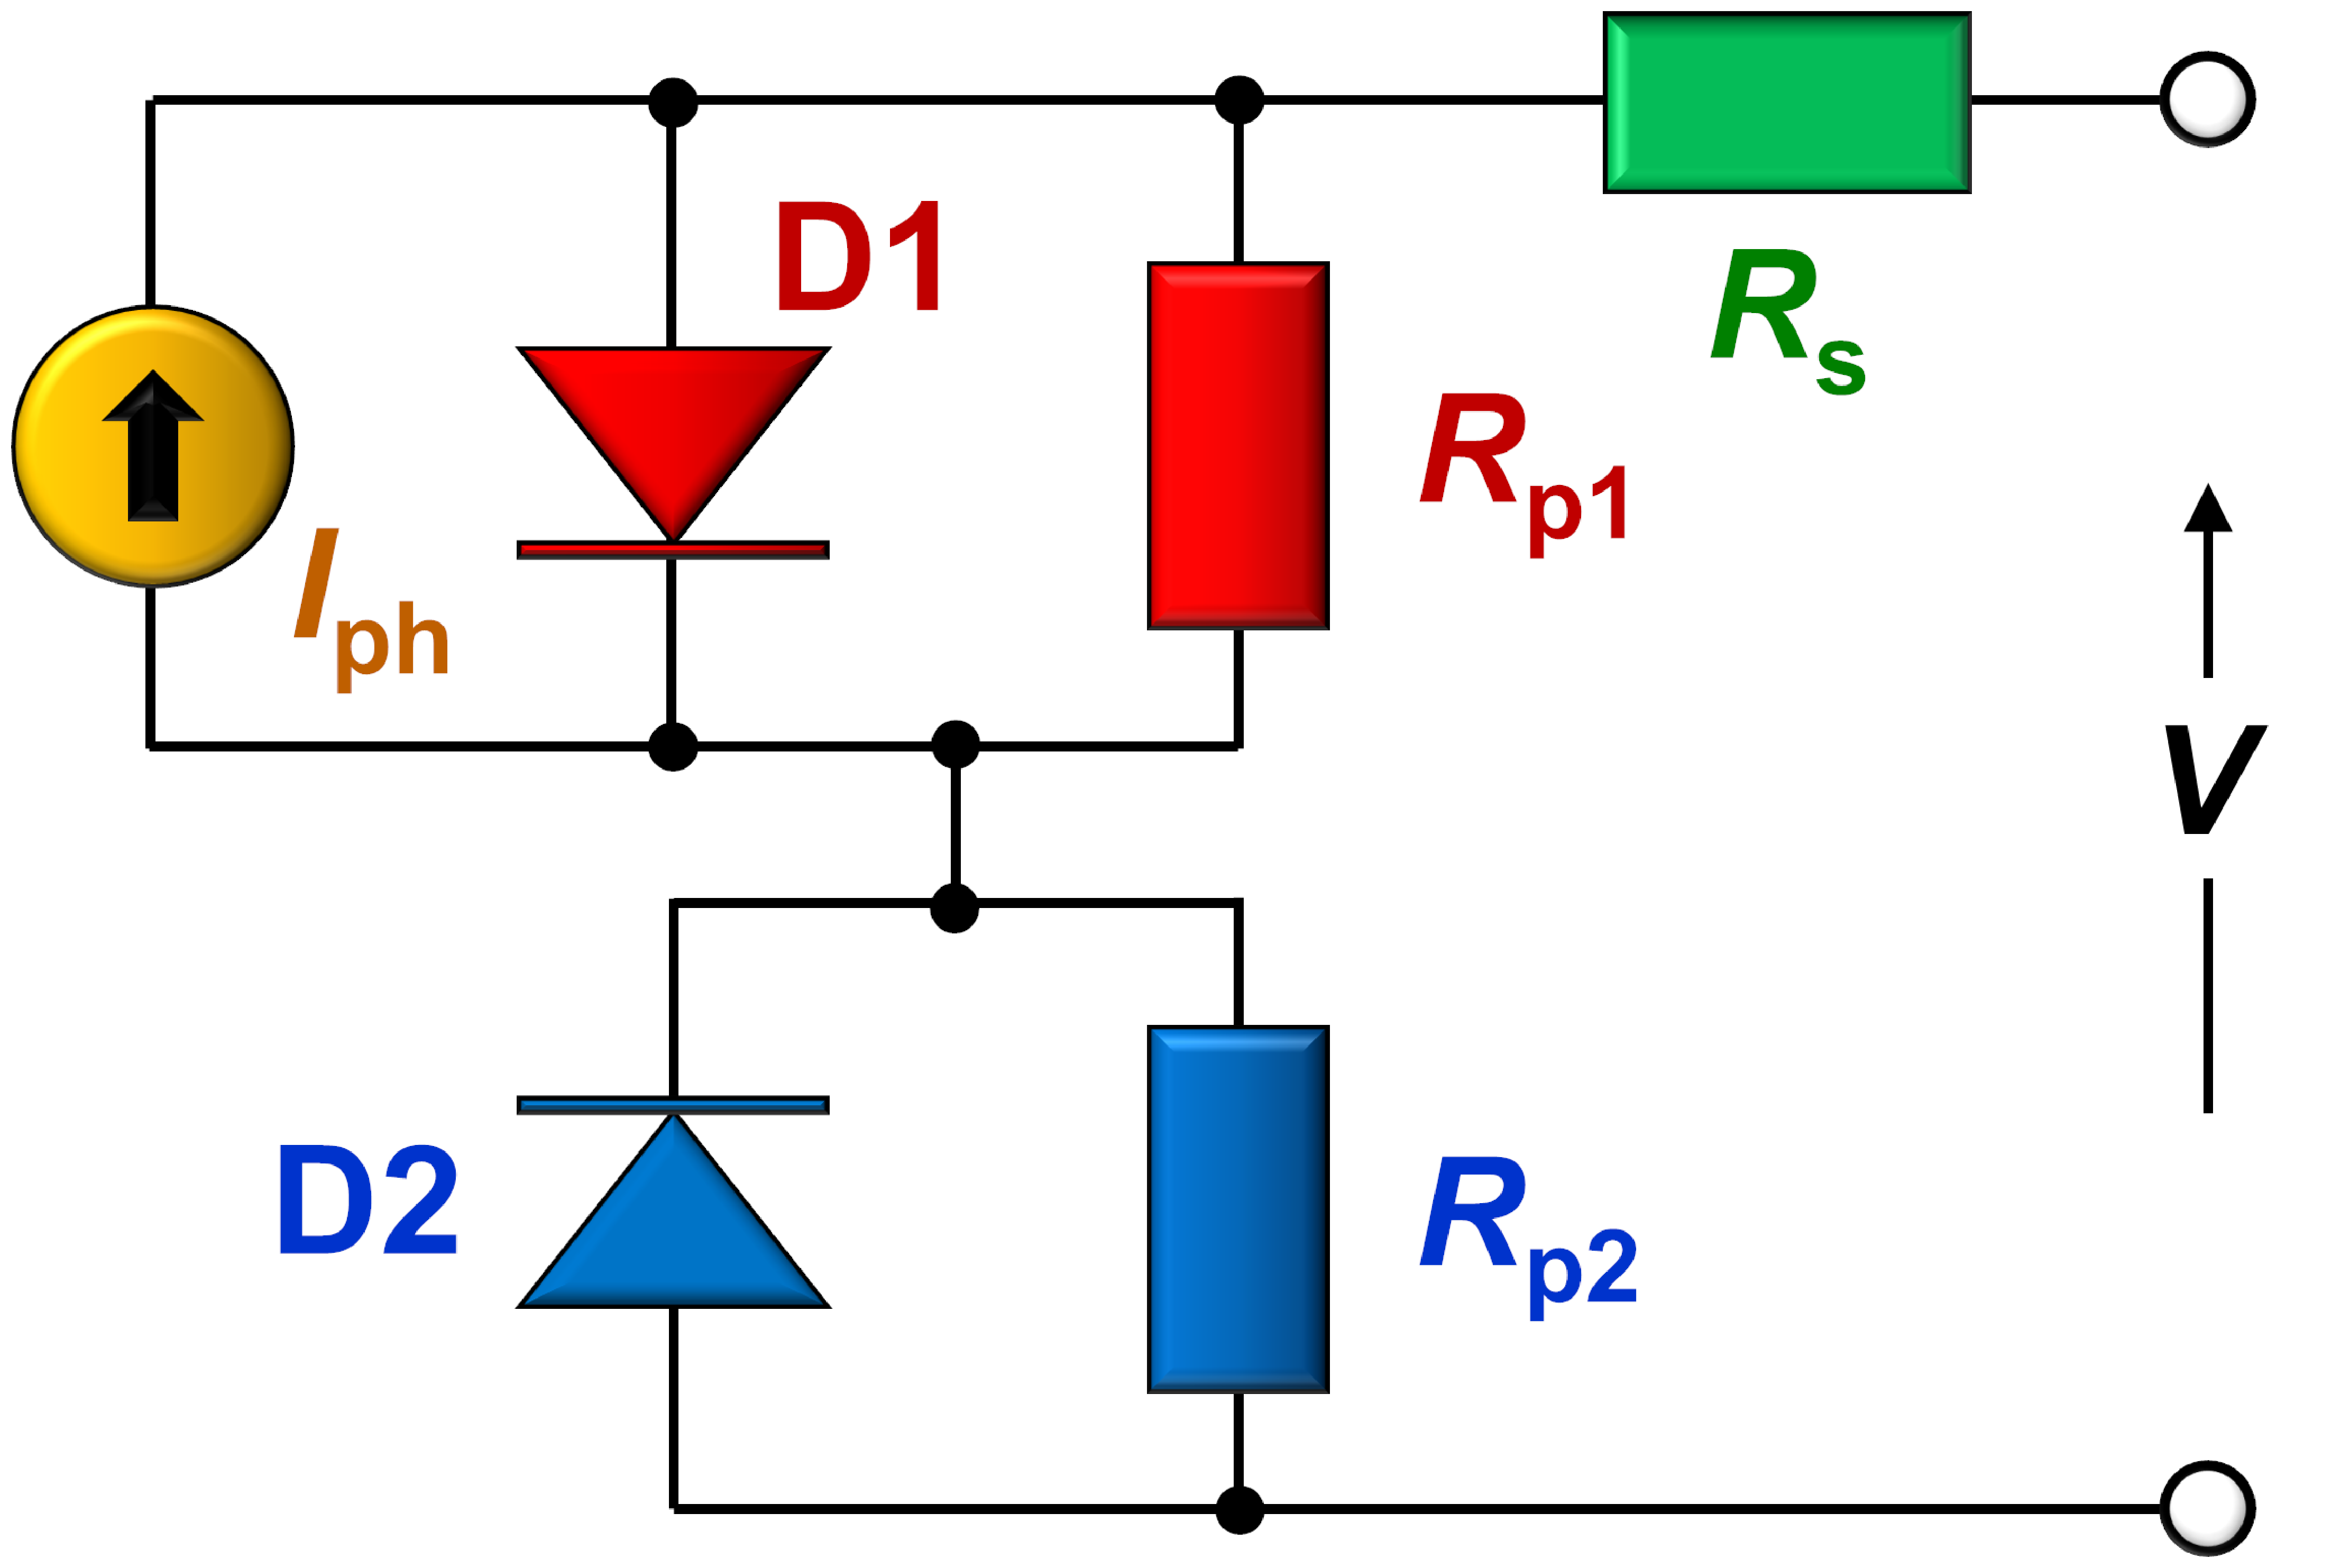
\includegraphics[width=0.9\columnwidth]{Chem}
	  \caption{The opposed two--diode equivalent--circuit model of a solar cell.}\label{fig_chem}
\end{figure}


\begin{eqnarray}
% \nonumber to remove numbering (before each equation)
\label{eqIV_W}
V&=& (I+I_\mathrm{ph}+I_{01})R_\mathrm{p1} \nonumber \\
  &&-\frac{n_1kT}{q}W\left\{\frac{qI_{01}R_\mathrm{p1}}{n_1kT}\exp\left[\frac{qR_\mathrm{p1}(I+I_\mathrm{ph}+I_{01})}{n_1kT}\right]\right\} \nonumber \\
  &&+\frac{n_2kT}{q}W\left\{\frac{qI_{02}R_\mathrm{p2}}{n_2kT}\exp\left[-\frac{qR_\mathrm{p2}(I-I_{02})}{n_2kT}\right]\right\} \nonumber \\
  &&+(I-I_{02})R_\mathrm{p2}+IR_\mathrm{s}\,,
\end{eqnarray}
where
$I_{01}$ and $I_{02}$ are the saturation currents and
$n_1$ and $n_2$ are
the ideality factors for D1 and D2 respectively,
and $I_\mathrm{ph}$ is the ideal photocurrent.
Thus, the model employs eight lumped parameters
($I_{01}$, $n_1$, $R_\mathrm{p1}$, $I_{02}$, $n_2$, $R_\mathrm{p2}$,
$R_\mathrm{s}$, and $I_\mathrm{ph}$)
that need to be determined from the I-V curve.
Thus, from an optimization perspective, the dimension of the problem is $D=8$.

The expression~(\ref{eqIV_W}) has a drawback in that it tends to stray from the range of numbers that can be accommodated by the standard 64-bit floating-point format owing to the presence of exponential functions for larger numbers.
To overcome this drawback, the use of the $g$--function $g(x)=\ln(W(\exp(x)))$ was suggested \cite{roberts2015calculating}.
The analytical solution $V(I)$ using the $g$--function is as follows \cite{roberts2015calculating}
\begin{equation}
\label{eqIV_g}
\begin{split}
V(I)= &IR_\mathrm{s}+\frac{n_1kT}{q}g(x_1)-\frac{n_2kT}{q}g(x_2) \\
  &-\frac{n_1kT}{q}\ln\left[\frac{qI_{01}R_\mathrm{p1}}{n_1kT}\right] +\frac{n_2kT}{q}\ln\left[\frac{qI_{02}R_\mathrm{p2}}{n_2kT}\right]\,,
\end{split}
\end{equation}
with
\begin{equation}
\label{eqx1}
x_1= \ln\left(\frac{qI_{01}R_\mathrm{p1}}{n_1kT}\right)+\frac{q(I+I_\mathrm{ph}+I_{01})R_\mathrm{p1}}{n_1kT}\,,
\end{equation}
and
\begin{equation}
\label{eqx2}
x_2= \ln\left(\frac{qI_{02}R_\mathrm{p2}}{n_2kT}\right)-\frac{q(I-I_{02})R_\mathrm{p2}}{n_2kT}\,.
\end{equation}
We used Eqs.~(\ref{eqIV_g})--(\ref{eqx2}) both for simulation IV curves and during the approximation procedure.
The $g$--function was evaluated by using iterative procedure \cite{roberts2015calculating}.

\subsection{Synthetic IV curves}\label{SynIV}
The research involved the parameter estimation of solar cells using meta-heuristic algorithms based
on synthetic IV characteristics simulated using the opposed two--diode model.
This approach allows for assessing the accuracy of the employed optimization methods,
as the simulation was performed using known parameter values.

In first part of the study, a detailed analysis was conducted on a single IV curve,
evaluating the performance of meta--heuristic algorithms for parameter estimation in a one--time application mainly.
Additionally, the suitability of employing two different fitness functions was examined.
In the second part, we simulated a set of IV characteristics and evaluated the average performance metrics of various algorithms.

\subsubsection{Single--IV case}\label{SingleIV}

Previous studies have demonstrated \cite{Tada2015Organic,Tada2021} that when the ideality factor of D2 is either equal to or significantly larger than $n_1$
($n_1=n_2=1.92$ or $n_1=1.00$, $n_2=3.00$), the nonlinear least--squares method successfully determines a set of equivalent circuit parameters
that accurately replicate the experimental data of an organic photovoltaic cell.
Therefore this approach does not allow for distinguishing between similar IV curves obtained from solar cells with different parameters.
To overcome this issue, Tada \cite{Tada2021} successfully employed Bayesian estimation of parameters.
To assess the capabilities of meta-heuristic methods in overcoming additional similar challenges,
they were applied to a IV curve corresponding to such a problematic case.
The parameter values were taken from \cite{Tada2021}:
\begin{equation}
\label{eqParSingleIV}
\begin{split}
I_{01}&=1.6\cdot10^{-6}\,\text{mA},\\
n_1&=1.92,\\
R_\mathrm{p1}&=190\,\Omega,\\
I_{02}&=0.16\,\text{mA},\\
n_2&=1.92,\\
R_\mathrm{p2}&=190\,\Omega,\\
R_\mathrm{s}&=45\,\Omega,\\
I_\mathrm{ph}&=8\,\text{mA},
\end{split}
\end{equation}
%($I_{01}=1.6\cdot10^{-6}$~mA,
%$n_1=1.92$,
%$R_\mathrm{p1}=190$~$\Omega$,
%$I_{02}=0.16$~mA,
%$n_2=1.92$,
%$R_\mathrm{p2}=190$~$\Omega$,
%$R_\mathrm{s}=45$~$\Omega$,
%$I_\mathrm{ph}=8$~mA),
and the IV curve was simulated over a range of 0-0.8~V with step 10~mV at $T=300$~K.
The simulation result is presented on Fig.~\ref{figSigleIV} by symbols.


\begin{figure}[]
	\centering
		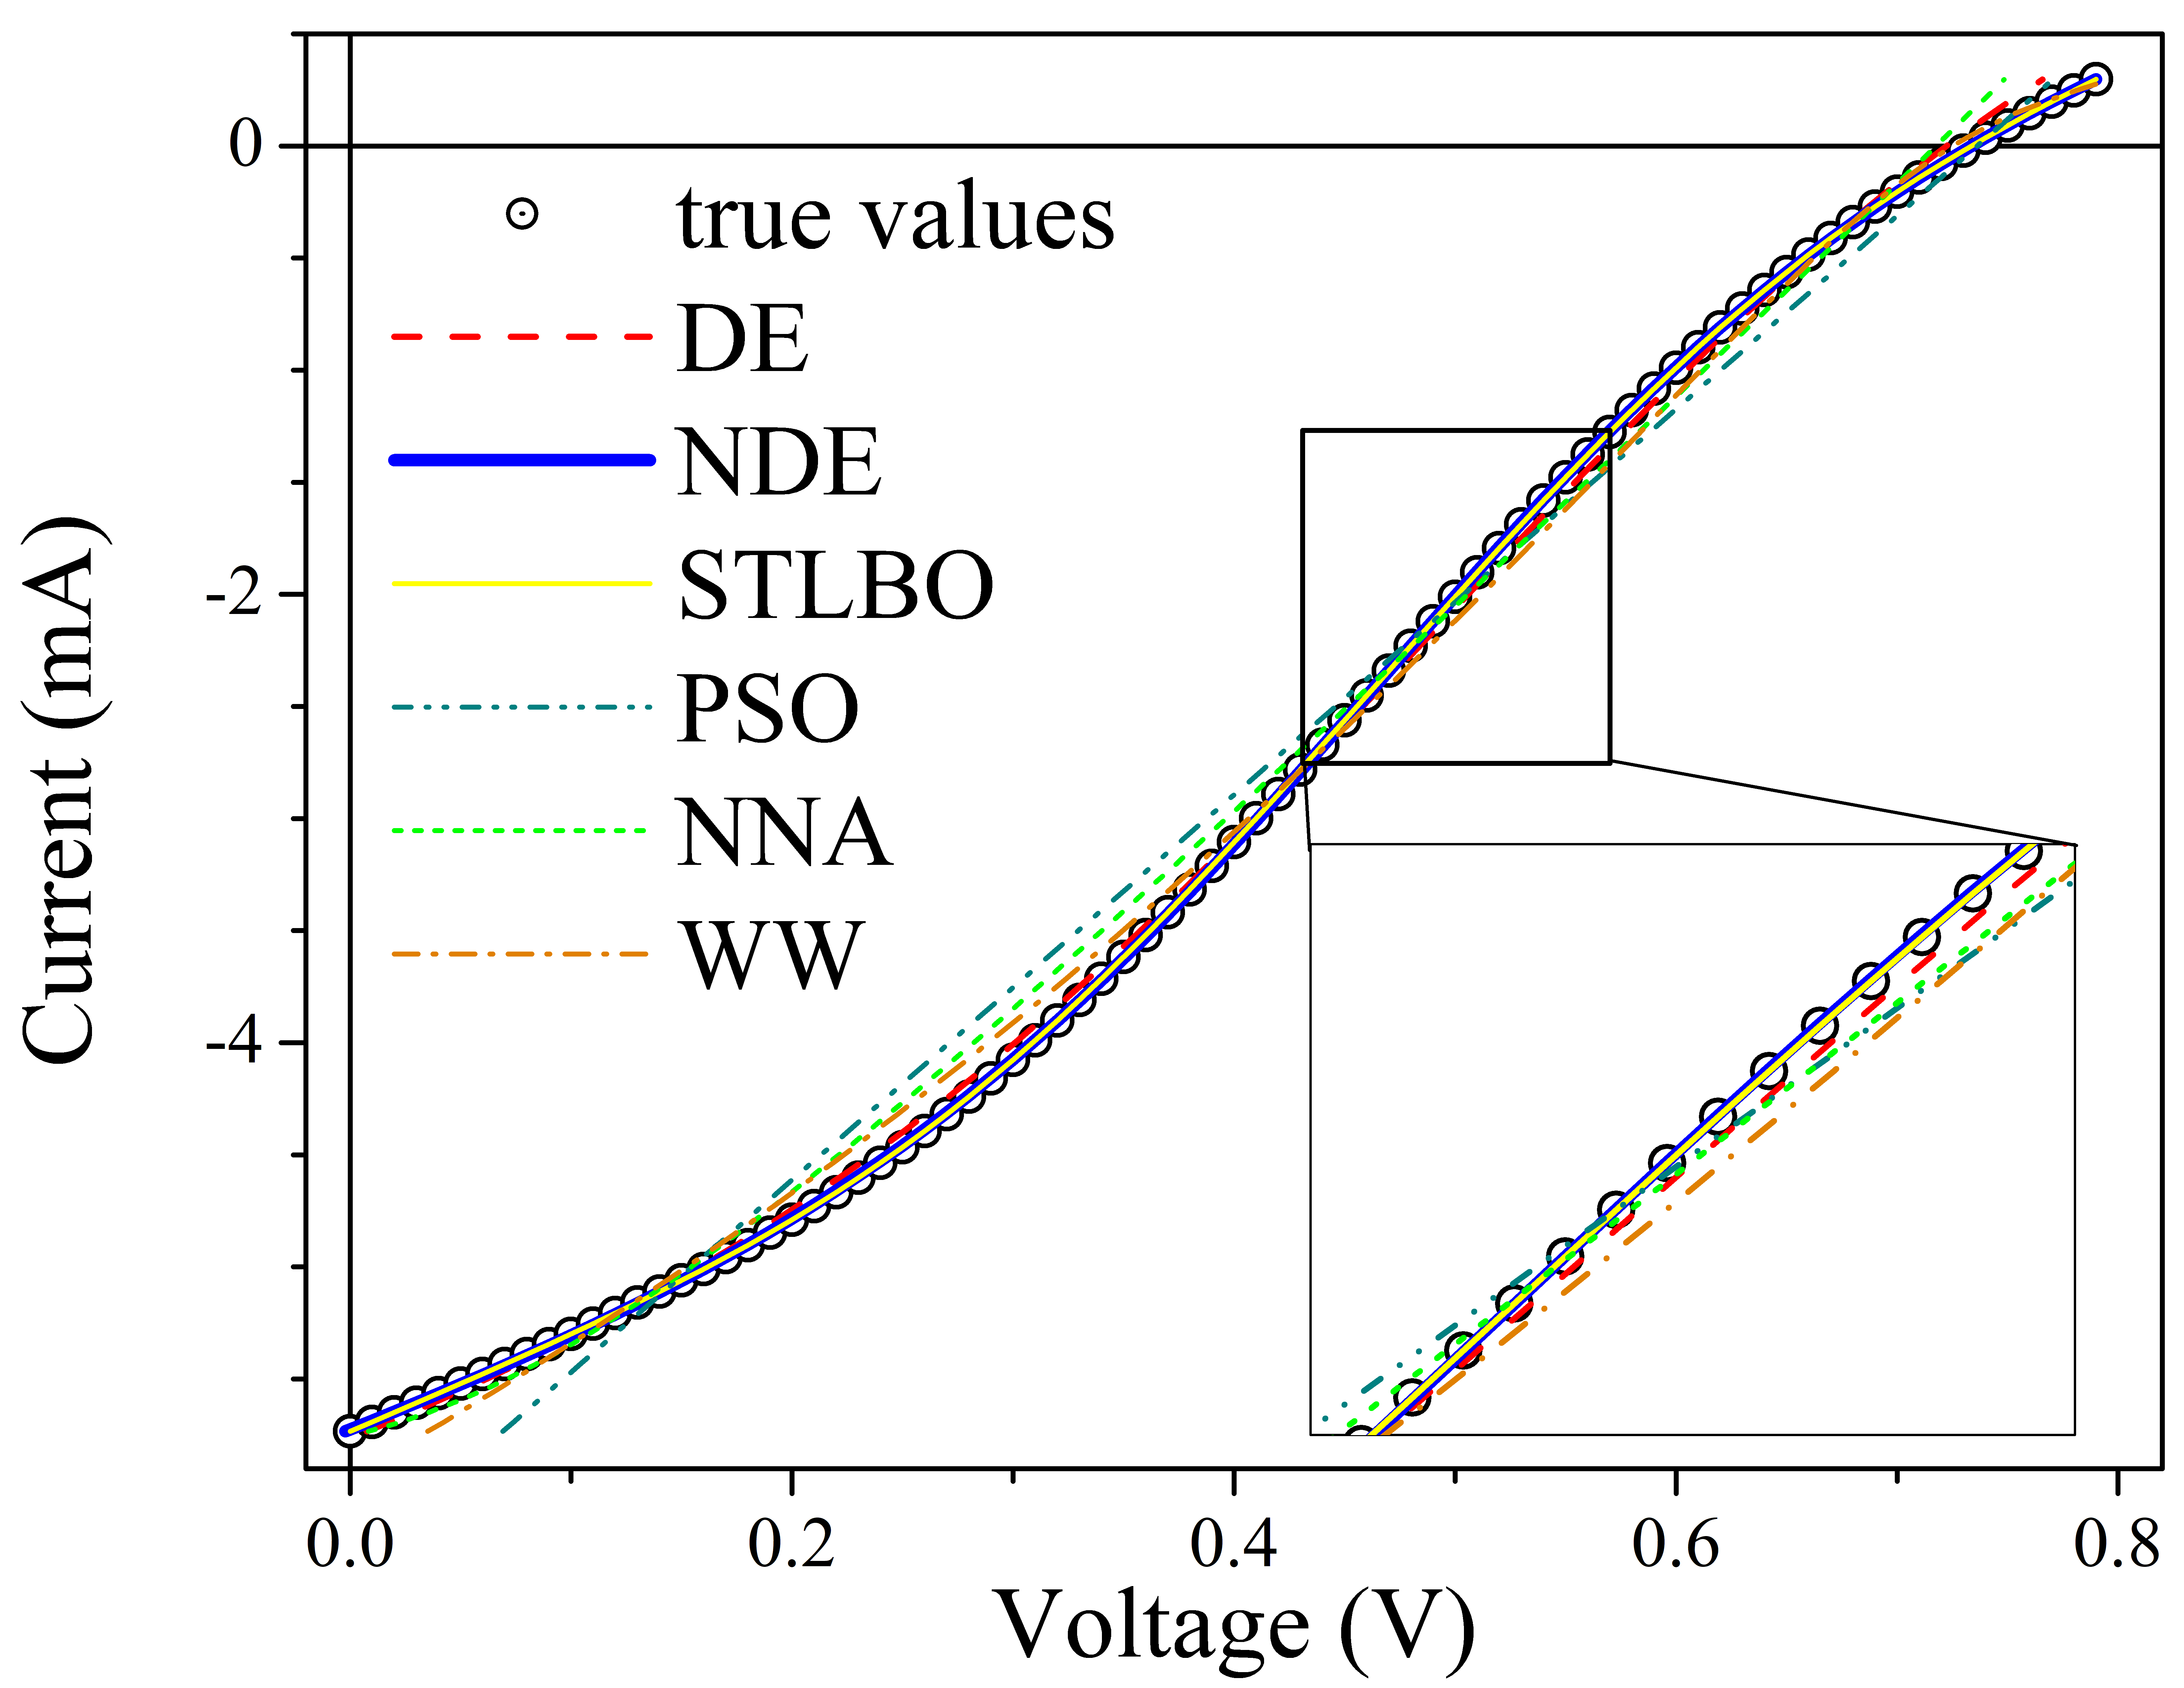
\includegraphics[width=1.0\columnwidth]{IVsimple}
	  \caption{Fitting results (lines) for the simulated current-voltage characteristic (symbols).
             The values from  Eq.~(\ref{eqParSingleIV}) were assumed under simulation.}\label{figSigleIV}
\end{figure}

%It has been shown previously whether the ideality factor of D2 ($n_2$) is the same as that of D1
%($n_1=n_2=1.92$) or very larger than $n_1$ ($n_1=1.00$, $n_2=3.00$),
%the nonlinear least--squares method finds a set of equivalent circuit parameters that reproduces the experimental
%data of an organic photovoltaic cell.


\subsubsection{IV--set case}\label{SetIV}
Employing various meta--heuristic algorithms to analyze a single IV curve
is insufficient to obtain comprehensive insights into the methods' efficacy in parameter estimation.
The accuracy of parameter determination is closely tied to their absolute values.
For instance, an increase in the $R_\mathrm{p}$ value can pose challenges for accurately estimating resistance
because the shunt will have a lesser impact on the overall shape of IV curve.
In addition, the ratio between the parameter values also plays a crucial role.

To test the methods across different parameter values, we generated synthetic data in a temperature range from 260 K to 350 K.
During the simulation process, we considered various temperature dependencies of the parameters.
We based our approach on known physical mechanisms but focused on achieving the diversity of parameter ratio
instead of attempting to replicate real--life photovoltaic converters precisely.
Furthermore, an S--shaped IV curve is observed in solar cells of various types,
and diverse charge transport mechanisms significantly complicate the selection of
the only possible temperature dependence for each of the eight model parameters.
Therefore, we assumed that the current conduction mechanism through D1 is close to tunneling,
and hence, $I_{01}$, $R_\mathrm{p1}$, and $(n_1kT)$ remain constant,
with $I_{01}=0.015$~mA, $R_\mathrm{p1}=10^4$~$\Omega$, $n_1kT=7$~eV.
In the case of D2, the thermionic emission current was suggested
and $I_{02}$ and $n_2$ increased and decreased, respectively, with temperature rise \cite{Sze2012}:
\begin{eqnarray}
%\label{eqIV_W}
I_{02}&=& I_{002}\exp\left(-\frac{E_I}{kT}\right)\,,\\
n_2&=&1+\frac{T^*}{T}\,,
\end{eqnarray}
where $I_{002}$, $E_I$, and $T^*$ are the constants which are independent of temperature.
The values of $I_{002}=500$~A, $E_I=0.40$~eV, and $T^*=500$~K were used.
For $R_\mathrm{p2}$, an exponential temperature dependence was employed,
as it is widely observed \cite{Kondratenko2019} in modern solar cells for the shunt resistance:
\begin{equation}
R_\mathrm{p2}=R_\mathrm{p20}\exp\left(\frac{E_R}{kT}\right)\,.
\end{equation}
with
$R_\mathrm{p20}=9$~m$\Omega$,
$E_R=0.32$~eV.
The linear temperature dependencies is expected for both $I_\mathrm{ph}$ \cite{Green2003,Eberle2021} and $R_\mathrm{s}$ \cite{Ibrahim2017,Bradaschia2019}:
\begin{equation}
y=y_{0}[1+\mathrm{TC}_y(T-300)]\,,
\end{equation}
where
$y=I_\mathrm{ph}$ or $R_\mathrm{s}$,
$y_0$ is the parameter value at room temperature,
$\mathrm{TC}_y$ is the temperature coefficient of parameter.
For most types of monocrystalline silicon solar cells, the $\mathrm{TC}_{I_\mathrm{ph}}$ typically ranges from around $-0.0004$~K$^{-1}$ \cite{TuanLe2021}.
However, as the base thickness decreases, the temperature coefficient can increase to $-0.0014$~K$^{-1}$ \cite{Dupre2016}.
For hydrogenated amorphous silicon solar cells, $\mathrm{TC}_{I_\mathrm{ph}}$ is equal to $-10^{-3}$~K$^{-1}$ \cite{Riesen2016}.
For organic solar cells, the temperature coefficient can reach a magnitude of $-0.003$~K$^{-1}$ \cite{Rana2018}.
During the simulation, we assumed $\mathrm{TC}_{I_\mathrm{ph}}=-10^{-3}$~K$^{-1}$.
Furthermore, the values of $I_\mathrm{ph0}=1$~mA,
$\mathrm{TC}_{R_\mathrm{s}}=0.02$~K$^{-1}$,
and $R_\mathrm{s0}=50$~$\Omega$ were used.



%Thus, the set of synthetic IV curves was generated using the following temperature dependencies of the parameters:
%\begin{equation}
%\label{eqParSetIV}
%\begin{split}
%I_{01}(T)[\text{mA}]&=0.015\,,\\
%n_1(T)&=(7kT)^{-1},\\
%R_\mathrm{p1}(T)[\Omega]&=10^4\,,\\
%I_{02}(T)[\text{mA}]&=10^3\exp\left(-\frac{0.40}{kT}\right)\,,\\
%n_2&=1.92,\\
%R_\mathrm{p2}&=190\,\Omega,\\
%R_\mathrm{s}&=45\,\Omega,\\
%I_\mathrm{ph}&=8\,\text{mA},
%\end{split}
%\end{equation}
The set of I–V data was composed of 10 curves,
which were simulated at 10~K intervals from 260 to 350~K;
in this case,
$n_1$,
$I_{02}$,
$n_2$,
$R_\mathrm{p2}$,
$R_\mathrm{s}$,
and $I_\mathrm{ph}$
varied
from 6.37 to 4.73,
from 9 to 880 $\mu$A,
from 2.92 to 2.43,
from $1.4\cdot10^4$ to 360~$\Omega$,
from 10 to 100~$\Omega$,
and from 0.96 to 1.05~mA, respectively.
The simulation results are presented on Fig.~\ref{figSetIV} by symbols.
\begin{figure}[]
	\centering
		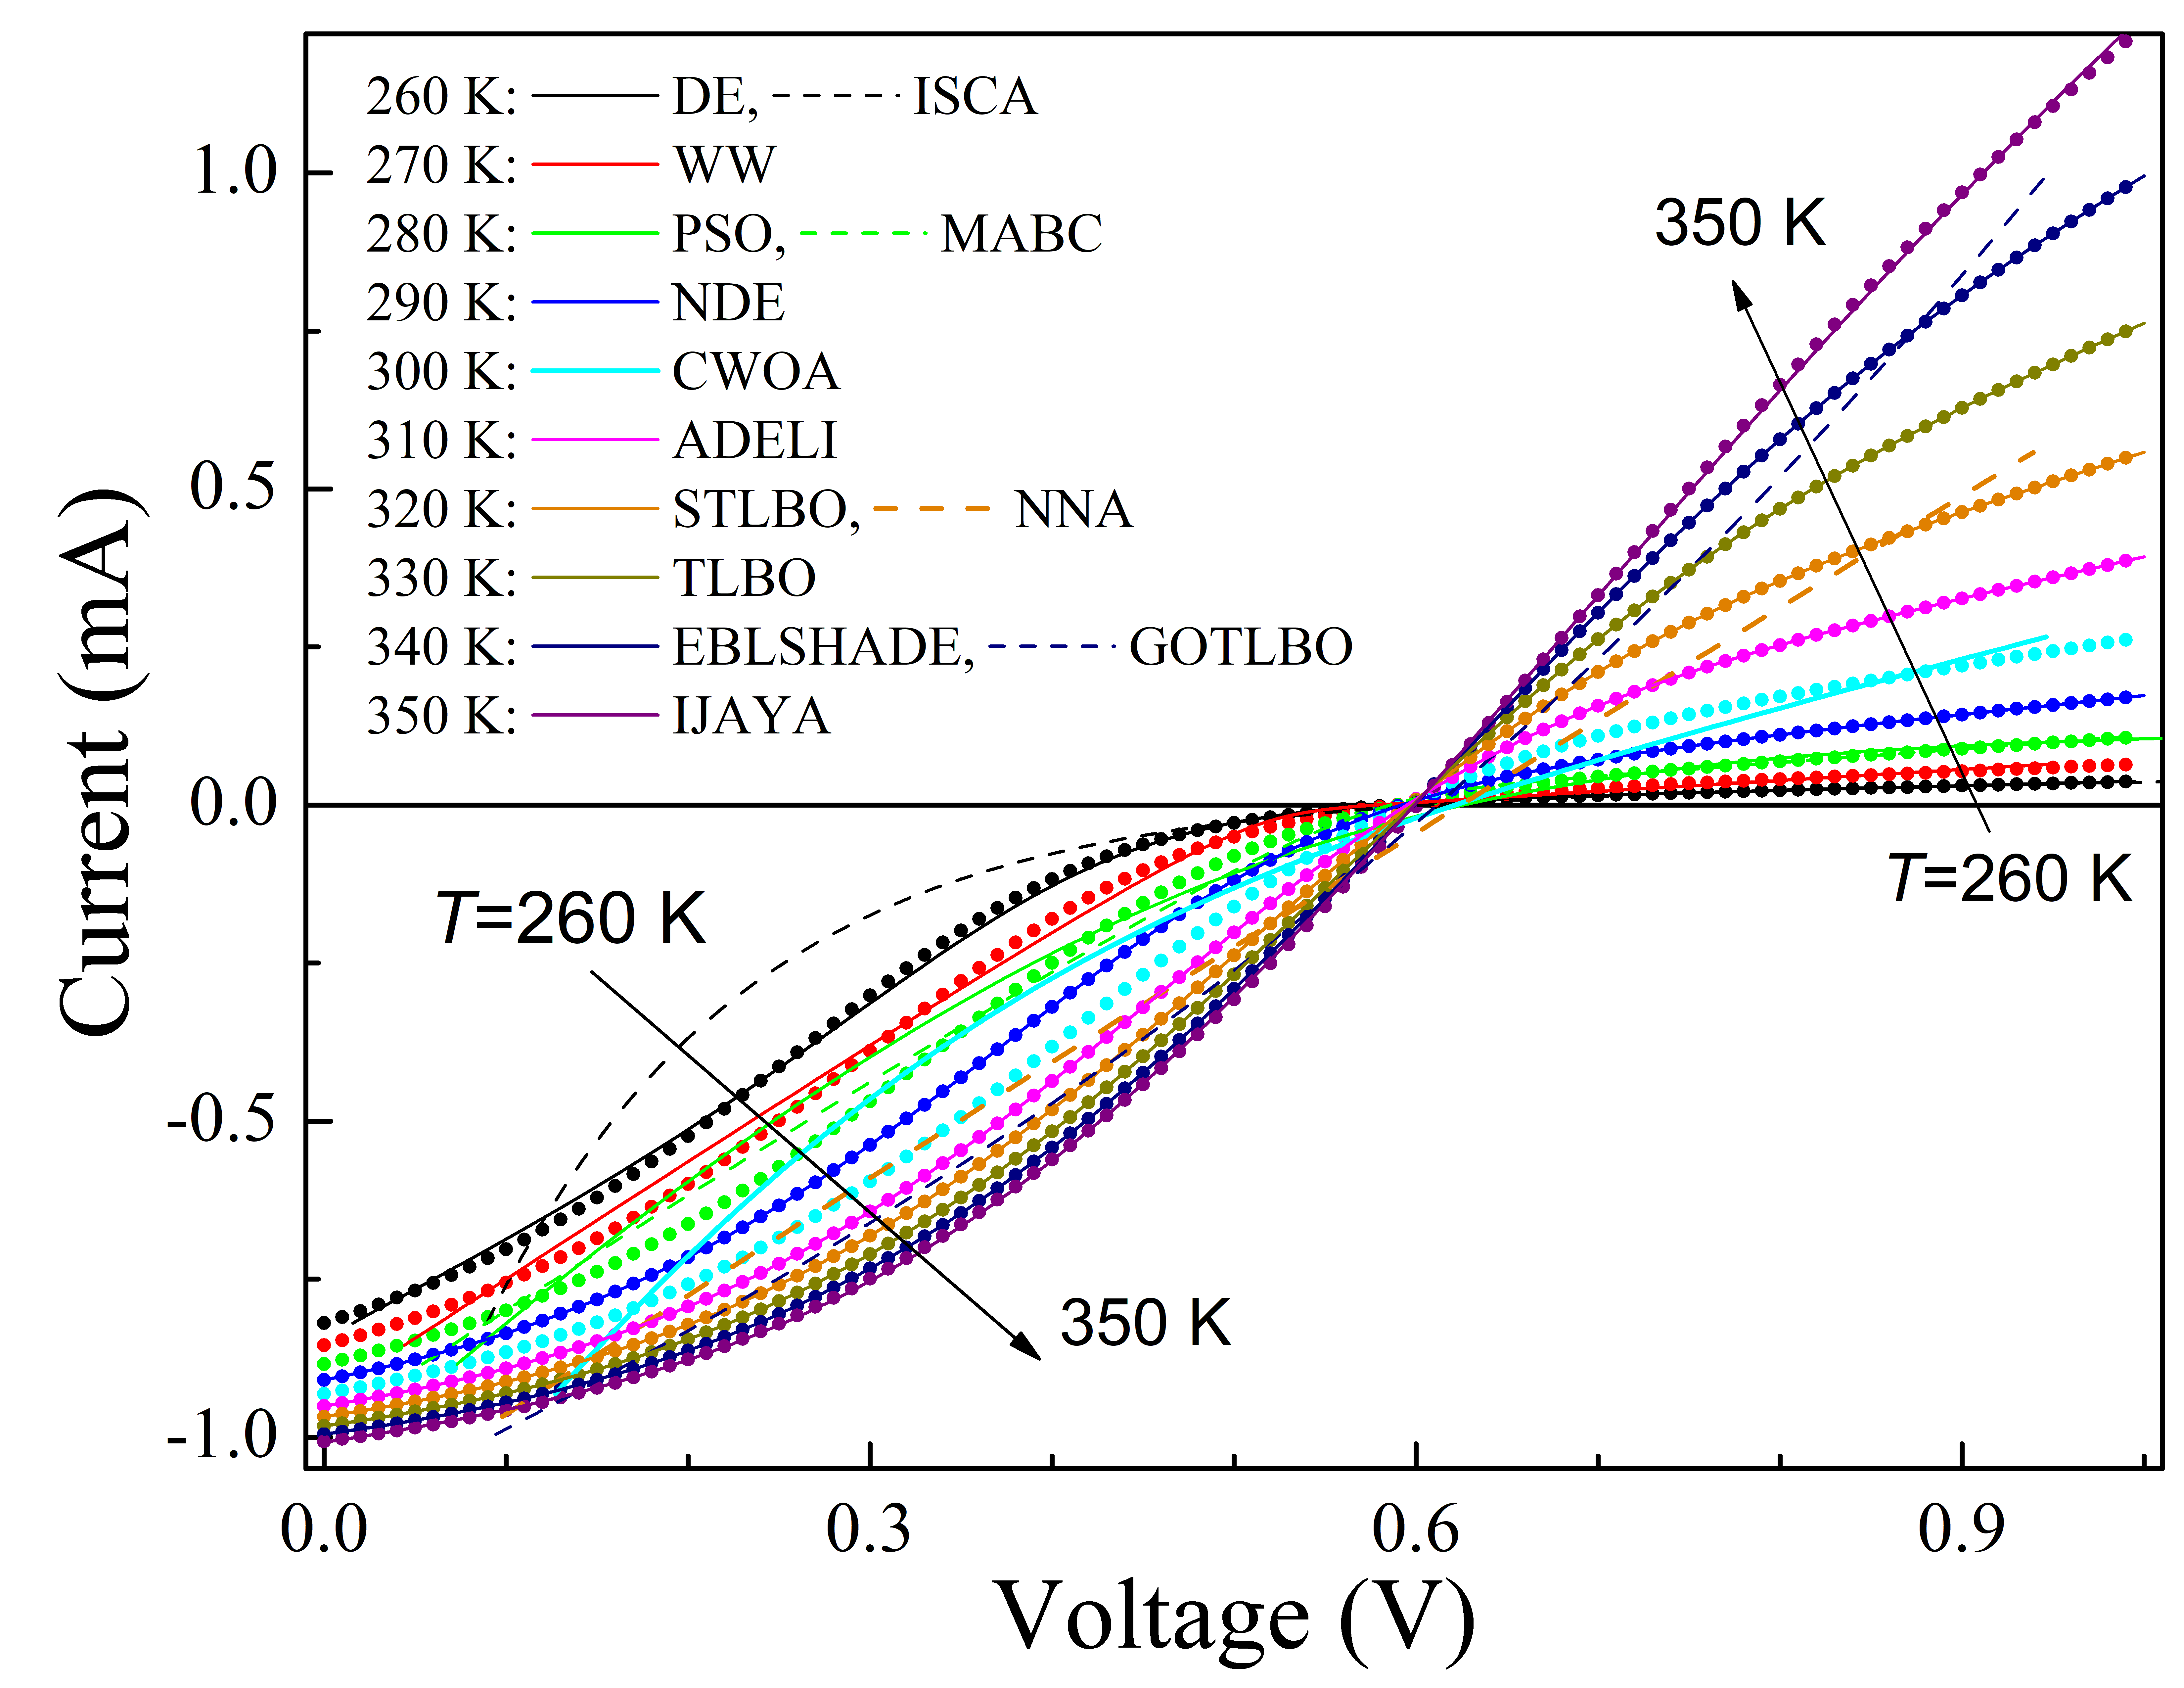
\includegraphics[width=1.0\columnwidth]{IVset}
	  \caption{Fitting results (lines) for the simulated current-voltage characteristic (symbols).
             The values from  Sec.~\ref{SetIV} were assumed under simulation.}\label{figSetIV}
\end{figure}

%перекласти на англійську "Таким чином, узагальнюючи, при створенні набору штучних ВАХ були використані наступні температурні залежності параметрів"



%виправити стилістичні помилки ""

%Estimation of parameters for solar cells with S--shaped current--voltage characteristics using meta--heuristic algorithms

\subsection{Meta-heuristic algorithms}\label{MHA}
In the literature, meta-heuristics are frequently categorized based on their sources of inspiration.
This categorization involves incorporating elements of true simulations and principles that incorporate stochasticity,
with the objective of emulating diverse characteristics observed in biological behavior, the lives of creatures in nature, human behavior, or natural phenomena.
On this basis, any meta-heuristic algorithm can fall into one of the following main classes \cite{WhiteShark,Gannet,Dandelion}:
evolution-based methods (emulate the principles of evolutionary behavior observed in creatures in nature by relying on the concept of survival of the fittest),
swarm intelligence--based methods (simulate the collective, dynamic, intelligent, and concerted gregarious conduct of collections of flocks or communities found in nature),
bio--based methods (use biological processes unrelated to group behavior),
chemical \& physical--based methods (originate from the physical phenomena or chemical laws that exist in the universe),
human-society--based methods (inspired by human beings, including various activities such as thinking and social behavior),
and math--based methods (borrow the mathematical functions).
Generally, there are hundreds of meta-heuristic optimization methods available.
While we acknowledge that our selection may not be fully comprehensive,
we utilized 14 methods, representing all classes mentioned above,
to tackle the parameter estimation task within the framework of the opposed two-diode model for a solar cell.
Hereafter, we provide a succinct description of each method alongside the parameters employed during the fitting process.

\emph{Differential evolution} (\textbf{DE}).
DE is one of the classical methods,
and  it is based on the natural selection law and uses the randomly generated initial population,
differential mutation, and probability crossover \cite{DEWang}.
During the implementation, we employed a penalty function suggested by Ishaque \emph{et al} \cite{P-DE_Ishaque}.
Besides, according to Wang and Ye \cite{DEWang}, the values of mutation scaling factor $F=0.8$,
crossover rate $C\!r=0.3$, and population size $N\!p=8\times D=64$ were used in this work.

\emph{Adaptive differential evolution with the Lagrange interpolation argument} (\textbf{ADELI}).
The method is based on DE, which integrates an adaptive local search scheme with Lagrange interpolation \cite{ADELI}.
This incorporation aims to enhance the exploitation capability and accelerate the convergence speed.
In ADELI, the scaling factor and crossover rate are set to self--adapting to optimize the results.
We used parameter values recommended by Huang \emph{et al} \cite{ADELI} during the implementation process.
Additionally, we set $N\!p$ to 64 for our numerical experiments.

\emph{Differential evolution with neighborhood--based adaptive evolution mechanism} (\textbf{NDE}).
The method uses a mutation strategy, which takes into account neighborhood and individual information, and an adaptive evolution mechanism \cite{NDE}.
The determination of $F$ and $C\!r$ values is achieved through the utilization of the weighted adaptive procedure \cite{Tanabe2014},
and an adaptive adjustment of the population size is implemented using a simple reduction method (from $10\times D=80$ to 5).

\emph{Success history based DE with hybridization mutation strategies and population size reduction} (\textbf{EBLSHADE}).
The method is the hybridization framework between \emph{pbest} and \emph{ord\_pbest} mutation strategies
and stores a set of $Cr$ and $F$ values that have performed well in the recent past \cite{EBLSHADE}.
A linear $N\!p$ reduction (from $18\times D=144$ to 4) is used as well.

\emph{Particle swarm optimization} (\textbf{PSO}).
It is another classic method based on observations of the social behavior of animals,
such as bird flocking, fish schooling, and swarm theory.
According to Ye et al. \cite{PSO},  the values of learning factors $l_1=l_2=2$,
the final weight and the initial weight $w_{max}=0.9$, $w_{min}=0.4$, and
$N\!p=15\times D=120$ are used in this work.

The \emph{modified artificial bee colony} (\textbf{MABC}) algorithm is based
on the intelligent foraging behavior of honey bee swarms \cite{MABC}.
The control parameters include the population size ($N\!p=8\times D=64$)
and the maximum number of generations after which each non-improved food source is to be discarded ($L_{imit}=36$).

\emph{Chaotic Whale Optimization Algorithm} (\textbf{CWOA}).
WOA draws inspiration from the hunting behavior of humpback whales \cite{WOA}.
On the other hand, CWOA employs chaotic maps to compute and dynamically adjust its internal parameters \cite{CWOA}.
In our study, we utilized the Singer chaotic map and set $N\!p=100$ for the identification of the parameters of the solar cell.

The \emph{Neural Network Algorithm} (\textbf{NNA}) is a meta-heuristic algorithm that draws inspiration from
both biological nervous systems and artificial neural networks \cite{NNA}.
The recommended \cite{NNA} value $N\!p=50$ is used in our paper.

The \emph{teaching learning based optimization} (\textbf{TLBO}) algorithm employs the concept of passing on knowledge
within a classroom.
Similar to learners acquiring knowledge from a teacher and interacting with their peers,
TLBO incorporates such interactions \cite{TLBO_Patel}.
In this study, a value of $N\!p=100$ is utilized.

\emph{Generalized oppositional teaching learning based optimization} (\textbf{GOTLBO}).
This method integrates a concept that incorporates both the current estimate
and its opposite estimate simultaneously into the original TLBO algorithm
through the initialization step and generation jumping \cite{GOTLBO}.
The values of jumping rate $J\!r=1.0$ and $N\!p=20$ were used.

\emph{Simplified teaching-learning based optimization algorithm} (\textbf{STLBO}).
In STLBO, an elite strategy is employed to improve the searching capability,
and a the chaotic map is used to enrich the uniformity of random values in the mutation phase \cite{STLBO}.
The logistic chaotic map and $N\!p=20$ were used.


\emph{Water wave optimization} (\textbf{WWO}) takes inspiration from shallow water wave models
and borrows ideas from wave propagation, refraction, and breaking \cite{WW}.
WWO is easy to implement with a small-size population, and there are four control parameters:
the maximum wave height $h_{max}$,
the wavelength reduction coefficient $\alpha$,
the breaking coefficient $\beta$,
and the maximum number $k_{max}$ of breaking directions.
According to Zheng \cite{WW}, we used
the values $h_{max}=6$, $\alpha=1.026$,  $N\!p=10$,
$k_{max}=\min(12,D/2)=4$, and $\beta$ linearly decreased from 0.25 to 0.001.

\emph{Improved JAYA} (\textbf{IJAYA}).
Jaya algorithm is based on the concept
that the solution obtained for a given problem should move toward the best solution and should
avoid the worst solution and does not require any algorithm-specific parameter \cite{JAYA}.
In IJAYA, a self-adaptive weight is introduced to adjust the tendency of approaching the best solution
and avoiding the worst solution;
an experience-based learning strategy is employed to maintain the population diversity and enhance the exploration ability,
and a chaotic elite learning method is proposed to refine the quality of the best solution in each generation \cite{IJAYA}.
The logistic chaotic map and $N\!p=4\times D=32$ were used.

\emph{Improved sine cosine algorithm} (\textbf{ISCA}).
SCA based on simulating the behaviors of sine and cosine mathematical functions \cite{SCA}.
ISCA implementation included a modified position-updating equation based on inertia weight
($w_{start}=1$, $w_{end}=1$),
a nonlinear conversion parameter strategy based on the Gaussian function
($a_{start}=2$, $a_{end}=0$) \cite{ISCA2},
the creation of the opposite population to jump out from the local optima with $J\!r=0.1$ \cite{ISCA3},
a greedy selection, and $N\!p=30$.

The majority of the utilized algorithms demonstrate excellent performance when
it comes to parameter estimation of solar cells within conventional models (single or double diode) \cite{CWOA,DEWang,GOTLBO,IJAYA,MABC,PSO,STLBO,TLBO_Patel,LSHADE,IWOA}.

In meta-heuristic optimization methods, the quality of the extracted parameters is evaluated using the fitness function at
every iteration.
In our investigation, absolute error and square error fitness functions were under consideration:
\begin{equation}
\label{eqFae}
F_\mathrm{AE}(Y)= \sum_{k=1}^p \left|V^\mathrm{tr}(I_k)-V^\mathrm{cal}(I_k,Y)\right|\,,
\end{equation}
\begin{equation}
\label{eqFse}
F_\mathrm{SE}(Y)= \sum_{k=1}^p \left[V^\mathrm{tr}(I_k)-V^\mathrm{cal}(I_k,Y)\right]^2\,,
\end{equation}
where
$V^\mathrm{tr}(I_k)$ is the simulated value of voltage at current $I_k$,
$V^\mathrm{cal}(I_k,Y)$ is the calculated values of voltage, which can be obtained
by Eqs.~(\ref{eqIV_g})--(\ref{eqx2}),
for given set of parameters (i.e. $Y = \{I_{01},n_1,R_\mathrm{p1},I_{02},n_2,R_\mathrm{p2},R_\mathrm{s},I_\mathrm{ph}\}$)
at current $I_k$,
and $p$ is the total number of voltage steps in the IV characteristic.



%Each algorithm was run 51 times with different random seed for each simulated IV curves.
%The numbers of independent algorithmic runs are equal to 51 on each simulated IV curve
%to generate the statistical results.
We executed each tested algorithm for $N_\mathrm{runs}=51$ independent runs on each simulated IV curve
to generate the statistical results.
The search ranges were set as follows:

\noindent
$I_{01}(\mathrm{mA})\in[10^{-13},1]$,
$n_1\in[0.5,50]$,
$R_\mathrm{p1}(\Omega)\in[10,10^6]$,
$I_{02}(\mathrm{mA})\in[10^{-7},10]$,
$n_2\in[0.5,50]$,
$R_\mathrm{p2}(\Omega)\in[10,5\cdot10^4]$,
$R_\mathrm{s}(\Omega)\in[0.1,1000]$,
$I_\mathrm{ph}(\mathrm{mA})\in[10^{-3},100]$.
%\begin{eqnarray}
%\label{eqSR}
%I_{01}(\mathrm{mA})&\in&[10^{-13},1]\nonumber, \\
%n_1&\in&[0.5,50]\nonumber, \\
%R_\mathrm{p1}(\Omega)&\in&[10,10^6]\nonumber, \\
%I_{02}(\mathrm{mA})&\in&[10^{-7},10]\nonumber, \\
%n_2&\in&[0.5,50]\nonumber, \\
%R_\mathrm{p2}(\Omega)&\in&[10,5\cdot10^4]\nonumber, \\
%R_\mathrm{s}(\Omega)&\in&[0.1,1000]\nonumber, \\
%I_\mathrm{ph}(\mathrm{mA})&\in&[10^{-3},100]\nonumber .
%\end{eqnarray}

\subsection{Evaluation metrics}\label{EvalCr}

To better show the performance differences between compared algorithms,
several evaluation metrics are considered, which can be described as follows:
\begin{enumerate}[1.]
\item
Mean value (MEAN), median value (MEDIAN), standard deviance (STD), and interquartile range (IQR)
for each two--diode model parameter $y$
($y$ is one of $\left\{I_{01}\right.$, $n_1$, $R_\mathrm{p1}$, $I_{02}$, $n_2$, $R_\mathrm{p2}$, $R_\mathrm{s}$, $\left.I_\mathrm{ph}\right\}$).
MEAN and MEDIAN are often used to measure the solution quality.
The closer the obtained MEAN and MEDIAN values are to the actual parameter values,
the closer the obtained solution is to the optimal solution.
To quantify, we used the  absolute percentage of error (APE):
\begin{equation}
\label{eqAPE}
\mathrm{APE}\,(y)= \left| \frac{y-y^\mathrm{tr}}{y^\mathrm{tr}}\right|\,,
\end{equation}
where
$y^\mathrm{tr}$ is the parameter value used during the IV curve simulation.
APE was calculated for $y_i$, obtained by one--run algorithm application ($\mathrm{APE}_i$),
MEAN ($\mathrm{APE}_\mathrm{MEAN}$), and MEDIAN ($\mathrm{APE}_\mathrm{MEDIAN}$).
Reducing STD and IQR result in a more stable algorithm performance.

\item
%Run time average $t_\mathrm{run}$: is the average run time in seconds for an
%individual optimizer on a IV curve.
Another evaluation criterion used to compare the algorithms’ performance is to compare their execution time.
We used average run time $t_\mathrm{run}$ in seconds for an
individual optimizer on one IV curve.

\item
Root mean square percentage of error (RMSPE) is a statistical measure that indicates
how well the fitted curve matches the actual IV curve:
\begin{equation}
\label{eqRMSPE}
\mathrm{RMSPE}= \sqrt{\frac{1}{p} \sum_{k=1}^p \left[\frac{V^\mathrm{tr}(I_k)-V^\mathrm{cal}(I_k,Y)}{V^\mathrm{tr}(I_k)} \right]^2}\,.
\end{equation}

\item
Wilcoxon signed-rank test is a nonparametric statistical test used for pairwise comparisons of algorithms.
This test assigns a rank to all the scores considered as one group and then sums the ranks of each group.

\item
Friedman, Friedman Aligned Ranks, and Quade tests are used for comparing the performance differences
among optimization algorithms
(multiple comparisons $1\times N$ with a control method).
Therefore, the average rankings of the algorithms according to the
tests are reported.
Besides, the post--hoc  Finner, Holm, Hochberg, and Holland procedures
are used to establish proper comparisons between each algorithm and a set of other algorithms.

\item
Multiple Comparison Test (Friedman) with Shaffer’s static, Nemenyi, and Holm procedures
are employed to compute all possible pairwise comparisons between groups ($N\times N$)
and identify the differences.

\end{enumerate}




\section{Numerical results and discussion}\label{Result}
%Results and analysis of the experiment

\subsection{Comparison of algorithms time}
In meta--heuristic algorithms, a different termination can be defined.
For instance, a termination condition can be a specific number of iterations $N_\mathrm{it}$,
constraints on the number of fitness function evaluations $N_\mathrm{FE}$,
a specific rate of precision,
a specific time,
no sign of change in solutions after a specific number of iterations,
or a combination of these cases \cite{IntelligentChaoticClonal}.
In this study, the primary focus was on the accuracy of parameter estimation.
Therefore to ensure that both exploration and exploitation processes could be fully realized
by each algorithm with an equal opportunity, the termination criterion used was the absence of changes in the solution.
Based on this condition, the required number of iterations $N_\mathrm{it}$ was determined,
and the corresponding calculation time was measured $t_\mathrm{run}$.
In addition, the $N_\mathrm{FE}$ was evaluated.

All the applied algorithms have been coded and implemented in Embarcadero\textregistered Delphi $10.3$ programming software.
The run time was estimated by using WinAPI-functions \emph{QueryPerformanceCounter()} and \emph{QueryPerformanceFrequency()}.
The experiments were performed on Windows 10 Pro 64-bit,
2.9 GHz AMD Ryzen 7 4800H CPU, and 8~GB RAM.

%перекласти на англійську "Тому для того, щоб дати кожному з алгоритмів шанс повністю реалізувати процеси exploration and exploitation, кретиріем зупинки був вибраний наступний"


\begin{table}[<options>]
\caption{Comparison of optimization algorithms for single IV curve parameter estimation}\label{tblRun}
\begin{tabular*}{\tblwidth}{@{}LCCC@{}}
\toprule
Algorithm  &  $N_\mathrm{it}$ & $N_\mathrm{FE}$ & $t_\mathrm{run}$ (s)\\ % Table header row
\midrule
DE & 8000& 1024000& $42\pm1$\\
EBLSHADE & 3000& 444600& $22\pm1$\\
ADELI & 12000& 1800000& $93\pm2$\\
NDE & 5000& 430000&$20.2\pm0.3$ \\
MABC & 8000& 1024000&$48\pm11$ \\
TLBO & 5000& 1000000&$56.1\pm0.3$ \\
GOTLBO & 6000& 360000&$15\pm1$ \\
STLBO & 13000& 273000&$13.8\pm0.3$ \\
PSO & 4000& 480000&$19\pm3$ \\
IJAYA & 30000& 960000&$37\pm1$ \\
ISCA & 5000& 150000&$6.5\pm0.1$ \\
NNA & 5000& 250000&$10.6\pm0.5$ \\
CWOA & 3000& 300000&$16.6\pm0.5$ \\
WW & 3000& 35000&$1.4\pm0.1$ \\
\bottomrule
\end{tabular*}
\end{table}

The obtained results are listed in Table~\ref{tblRun}.
As can be seen from the table, the number of iterations required for an algorithm does not always correlate directly
with the number of fitness function evaluations or computation time needed to converge.
The reason is the unique features of each algorithm.
The run time of the algorithms varies considerably, with a range of 1.5 seconds to 93 seconds.
Notably, WW, ISCA, NNA, and STLBO converge the fastest, while ADELI, TLBO, and MABC require the most time.

\subsection{Fitness function selection}

To choose the more suitable fitness function, we evaluated each algorithm using the IV curve generated from the parameters
provided in Eq.~(\ref{eqParSingleIV}) with both $F_\mathrm{AE}$ and $F_\mathrm{SE}$ functions (see Eqs.~(\ref{eqFae}) and (\ref{eqFse})).
Afterward, the results obtained using each of the functions were compared through pairwise comparisons.
Table~\ref{tblFF} gives the statistical results produced by Wilcoxon sign-rank test with a significant level $\alpha = 0.05$.
A cell marked with the symbol ``SE'' indicates that evaluation of parameter specified in the column by the algorithm with $F_\mathrm{SE}$ outperforms result obtained by this  algorithm with $F_\mathrm{AE}$.
A cell marked with the symbol ``AE'' indicates better results for function $F_\mathrm{AE}$.
In the case of the symbol ``='', there is no significant difference between function $F_\mathrm{SE}$ and function $F_\mathrm{AE}$ aplication.


%\newcolumntype{G}{>{\columncolor{ligthGreen}}C}
%\newcolumntype{Y}{>{\columncolor{ligthYellow}}C}


\begin{table}[<options>]
\caption{Wilcoxon signed ranks test results of fitness functions comparison with a level of significance $\alpha = 0.05$}\label{tblFF}
\begin{tabular*}{\tblwidth}{@{}LCCCCCCCCC@{}}
\toprule
\multirow{2}{*}{Algorithm}& \multicolumn{9}{C}{Parameter} \\
  & $I_{01}$& $n_1$ & $R_\mathrm{p1}$ &$I_{02}$& $n_2$& $R_\mathrm{p2}$&$R_\mathrm{s}$&$I_\mathrm{ph}$&RMSPE\\ % Table header row
\midrule
%\rowcolor{ligthYellow}
DE &\cellcolor{ligthRed}SE &\cellcolor{ligthRed}SE &\cellcolor{ligthYellow}= & \cellcolor{ligthYellow}= &\cellcolor{ligthRed}SE &\cellcolor{ligthRed}SE &\cellcolor{ligthYellow}=  &\cellcolor{ligthYellow}=  &\cellcolor{ligthYellow}= \\
EBLSHADE &\cellcolor{ligthRed}SE &\cellcolor{ligthYellow}=  &\cellcolor{ligthYellow}=  &\cellcolor{ligthYellow}=  &\cellcolor{ligthYellow}=  &\cellcolor{ligthYellow}=  &\cellcolor{ligthYellow}=  &\cellcolor{ligthYellow}=  &\cellcolor{ligthBlue} AE \\
ADELI &\cellcolor{ligthRed}SE &\cellcolor{ligthYellow}=  & \cellcolor{ligthYellow}= & \cellcolor{ligthYellow}= & \cellcolor{ligthYellow}= & \cellcolor{ligthYellow}= &\cellcolor{ligthYellow}=  &\cellcolor{ligthYellow}=  & \cellcolor{ligthBlue} AE\\
NDE &\cellcolor{ligthYellow}=  &\cellcolor{ligthYellow}=  &\cellcolor{ligthYellow}=  &\cellcolor{ligthYellow}=  &\cellcolor{ligthYellow}=  &\cellcolor{ligthYellow}=  & \cellcolor{ligthYellow}= &\cellcolor{ligthRed}SE &\cellcolor{ligthRed}SE \\
MABC & \cellcolor{ligthYellow}= &\cellcolor{ligthRed}SE &\cellcolor{ligthYellow}=  & \cellcolor{ligthYellow}= &\cellcolor{ligthYellow}=  &\cellcolor{ligthYellow}=  &\cellcolor{ligthYellow}=  &\cellcolor{ligthYellow}=  &\cellcolor{ligthRed}SE \\
TLBO &\cellcolor{ligthRed}SE &\cellcolor{ligthRed}SE &\cellcolor{ligthRed}SE & \cellcolor{ligthRed}SE& \cellcolor{ligthRed}SE&\cellcolor{ligthRed}SE &\cellcolor{ligthRed}SE &\cellcolor{ligthRed}SE &\cellcolor{ligthRed}SE \\
GOTLBO &\cellcolor{ligthYellow}=  &\cellcolor{ligthYellow}=  &\cellcolor{ligthYellow}=  &\cellcolor{ligthYellow}=  &\cellcolor{ligthYellow}=  &\cellcolor{ligthRed}SE &\cellcolor{ligthYellow}=  &\cellcolor{ligthYellow}=  &\cellcolor{ligthYellow}=  \\
STLBO &\cellcolor{ligthRed}SE &\cellcolor{ligthYellow}=  &\cellcolor{ligthYellow}=  &\cellcolor{ligthYellow}=  &\cellcolor{ligthYellow}=  &\cellcolor{ligthYellow}=  &\cellcolor{ligthYellow}=  &\cellcolor{ligthYellow}=  &\cellcolor{ligthBlue} AE \\
PSO &\cellcolor{ligthYellow}=  &\cellcolor{ligthYellow}=  &\cellcolor{ligthYellow}=  &\cellcolor{ligthYellow}=  &\cellcolor{ligthYellow}=  &\cellcolor{ligthYellow}=  &\cellcolor{ligthBlue} AE &\cellcolor{ligthYellow}=  &\cellcolor{ligthYellow}=  \\
IJAYA &\cellcolor{ligthBlue} AE &\cellcolor{ligthBlue} AE & \cellcolor{ligthYellow}= &\cellcolor{ligthYellow}=  &\cellcolor{ligthRed}SE & \cellcolor{ligthYellow}= & \cellcolor{ligthYellow}= &\cellcolor{ligthYellow}=  &\cellcolor{ligthYellow}=  \\
ISCA &\cellcolor{ligthYellow}=  &\cellcolor{ligthYellow}=  &\cellcolor{ligthYellow}=  &\cellcolor{ligthYellow}=  &\cellcolor{ligthYellow}=  &\cellcolor{ligthYellow}=  &\cellcolor{ligthYellow}=  &\cellcolor{ligthYellow}=  &\cellcolor{ligthYellow}=  \\
NNA &\cellcolor{ligthYellow}=  &\cellcolor{ligthYellow}=  &\cellcolor{ligthYellow}=  &\cellcolor{ligthYellow}=  &\cellcolor{ligthYellow}=  &\cellcolor{ligthYellow}=  &\cellcolor{ligthYellow}=  &\cellcolor{ligthYellow}=  & \cellcolor{ligthRed}SE\\
CWOA &\cellcolor{ligthYellow}=  &\cellcolor{ligthYellow}=  & \cellcolor{ligthRed}SE&\cellcolor{ligthYellow}=  & \cellcolor{ligthBlue} AE&\cellcolor{ligthYellow}=  &\cellcolor{ligthYellow}=  &\cellcolor{ligthYellow}=  &\cellcolor{ligthRed}SE \\
WW &\cellcolor{ligthYellow}=  &\cellcolor{ligthYellow}=  & \cellcolor{ligthRed}SE& \cellcolor{ligthYellow}= &\cellcolor{ligthBlue} AE & \cellcolor{ligthYellow}= &\cellcolor{ligthYellow}=  &\cellcolor{ligthYellow}=  & \cellcolor{ligthRed}SE\\
\bottomrule
\end{tabular*}
\end{table}

As evidenced in the provided data, utilizing the square error fitness function more frequently yields better outcomes in comparison to $F_\mathrm{AE}$.
In rare cases, the absolute error fitness function can enhance the alignment between the fitted and actual curves,
as well as improve the accuracy of some parameter evaluations by PSO, IJAVA, CWOA, and WW algorithms.
However, RMSPE is not the most crucial factor in determining model parameters, and the mentioned methods,
as will be shown later, do not provide the highest accuracy.
As such, the results presented in the following sections are exclusive to the application of the $F_\mathrm{SE}$ function.
Therefore, it can be recommended that researchers consider
the square error fitness function as a more effective and reliable option for the task of opposed two--diode model parameter evaluation.

%Estimation of parameters for solar cells with S--shaped current--voltage characteristics using meta--heuristic algorithms

\subsection{Performance comparison}

\subsubsection{Evaluation of single--IV}

In this subsection, we show and analyze the statistical results of different meta-heuristic algorithm
applications to an IV curve, simulated with Eq.~(\ref{eqParSingleIV}) values.
Several typical fitting results of the synthesized curve are shown in Fig.~\ref{figSigleIV}.
A more comprehensive version, including the fitting results obtained using each algorithm,
is provided in the supplementary materials (figure S1).
It can be seen, that the closest match between the approximation curves and the IV curve points is
observed for EBLSHADE, ADELI, NDE, IJAYA, TLBO, and STLBO.
On the contrary, the PSO and GOTLBO fitting curves had the least replication of the original data.

Fig.~\ref{figBoxSingleIV} shows the results of cell parameters evaluation by comparative algorithms.
In addition, the figure presents the RMSPE data,
which confirms the conclusions of the visual comparison between the fitting lines and the points of the IV curve.
The results in terms of MEAN, MEDIAN, STD, and IQR are tabulated as well (table~S1 in the supplementary material).


\begin{figure*}[]
	\centering
		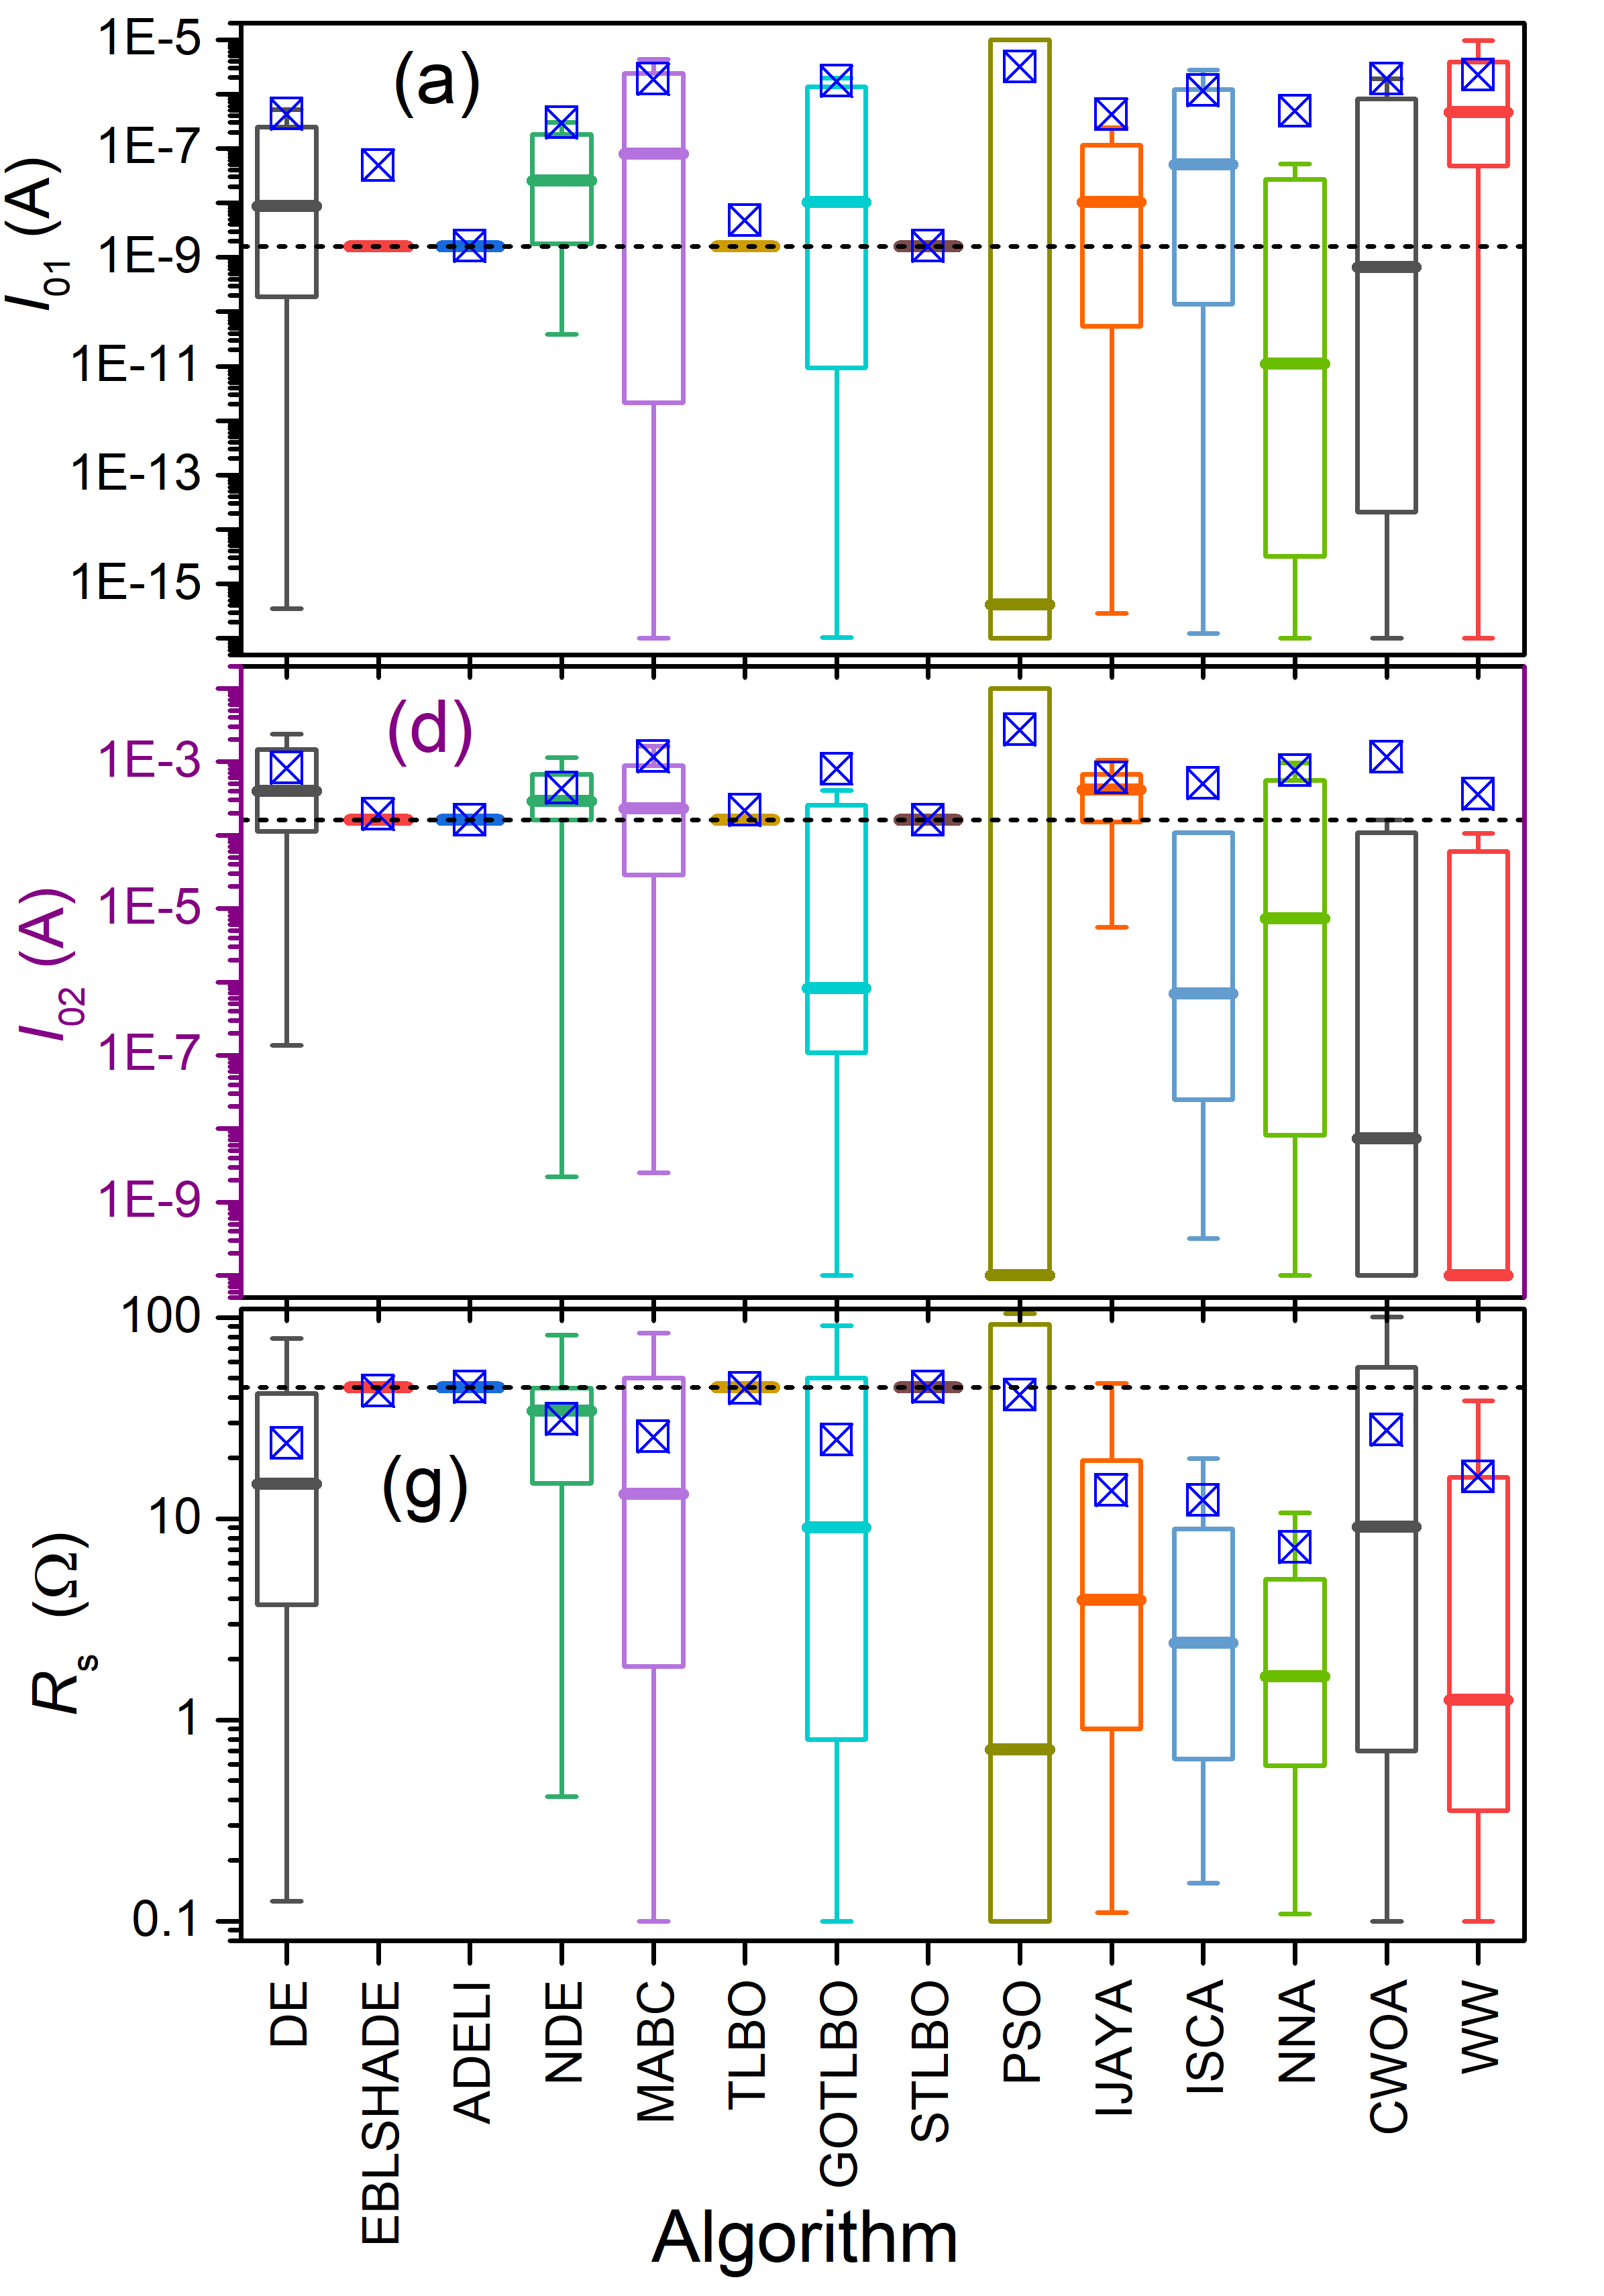
\includegraphics[width=.32\textwidth]{Fig3a}
        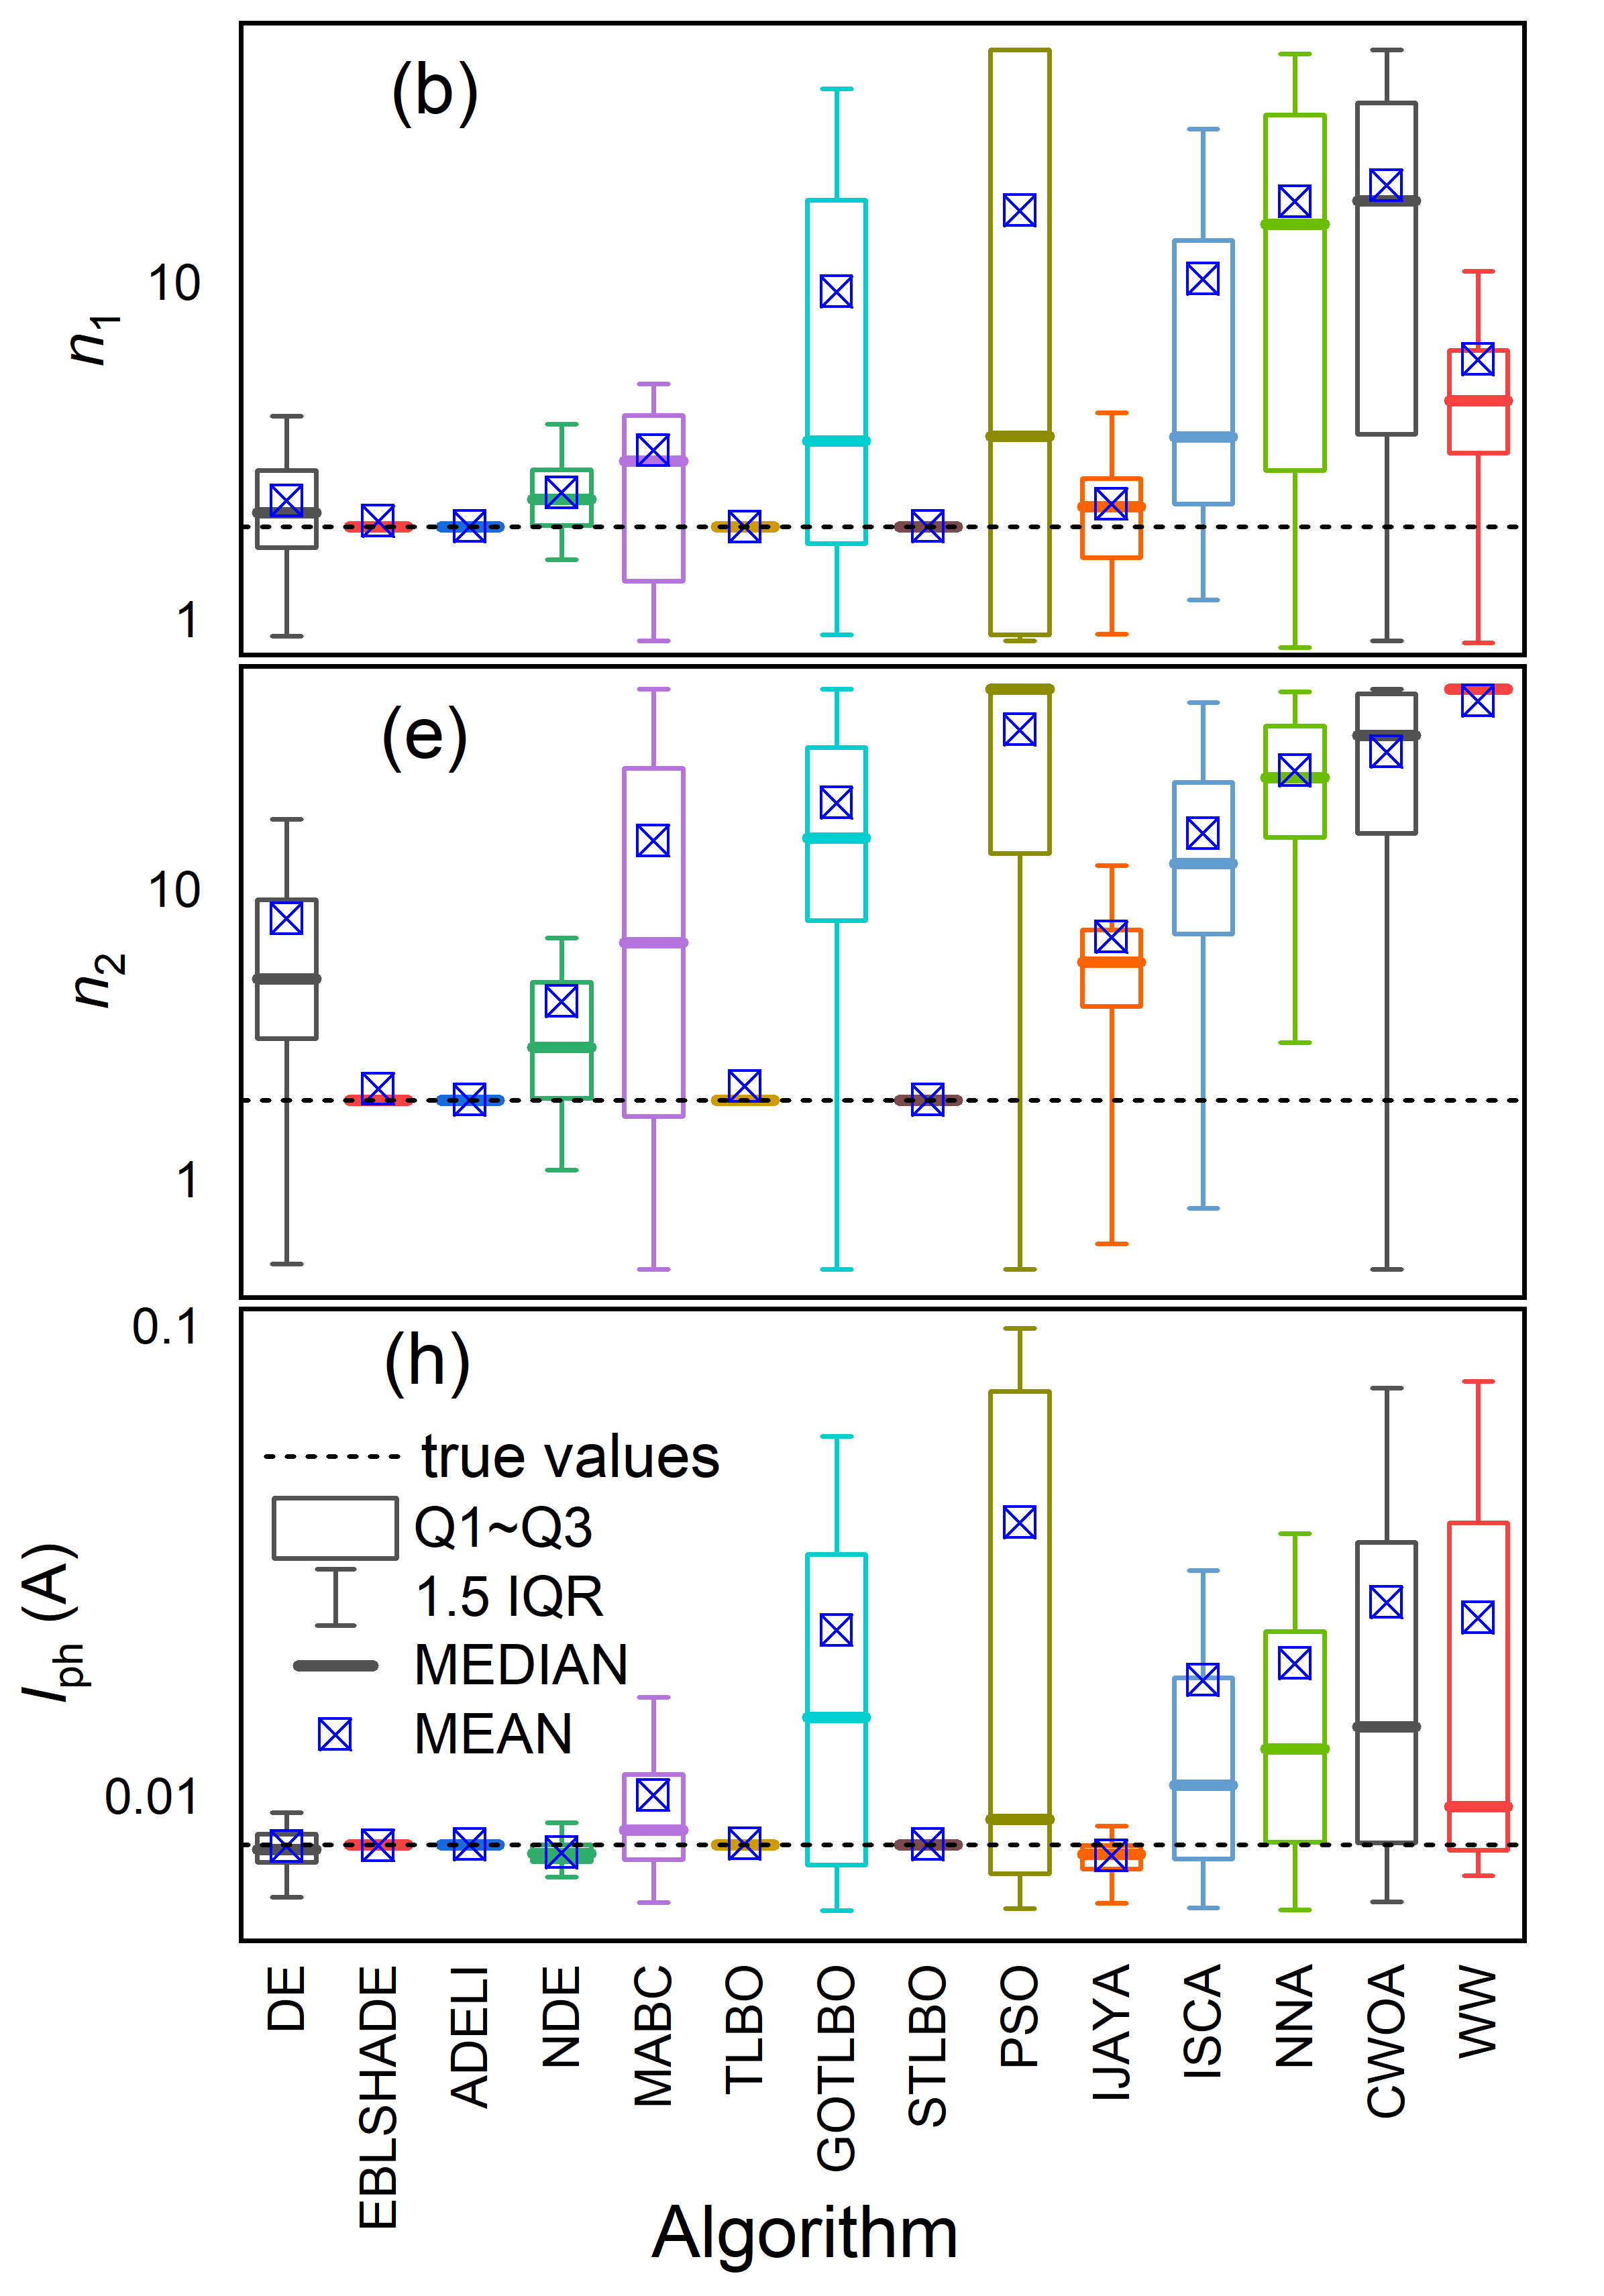
\includegraphics[width=.32\textwidth]{Fig3b}
        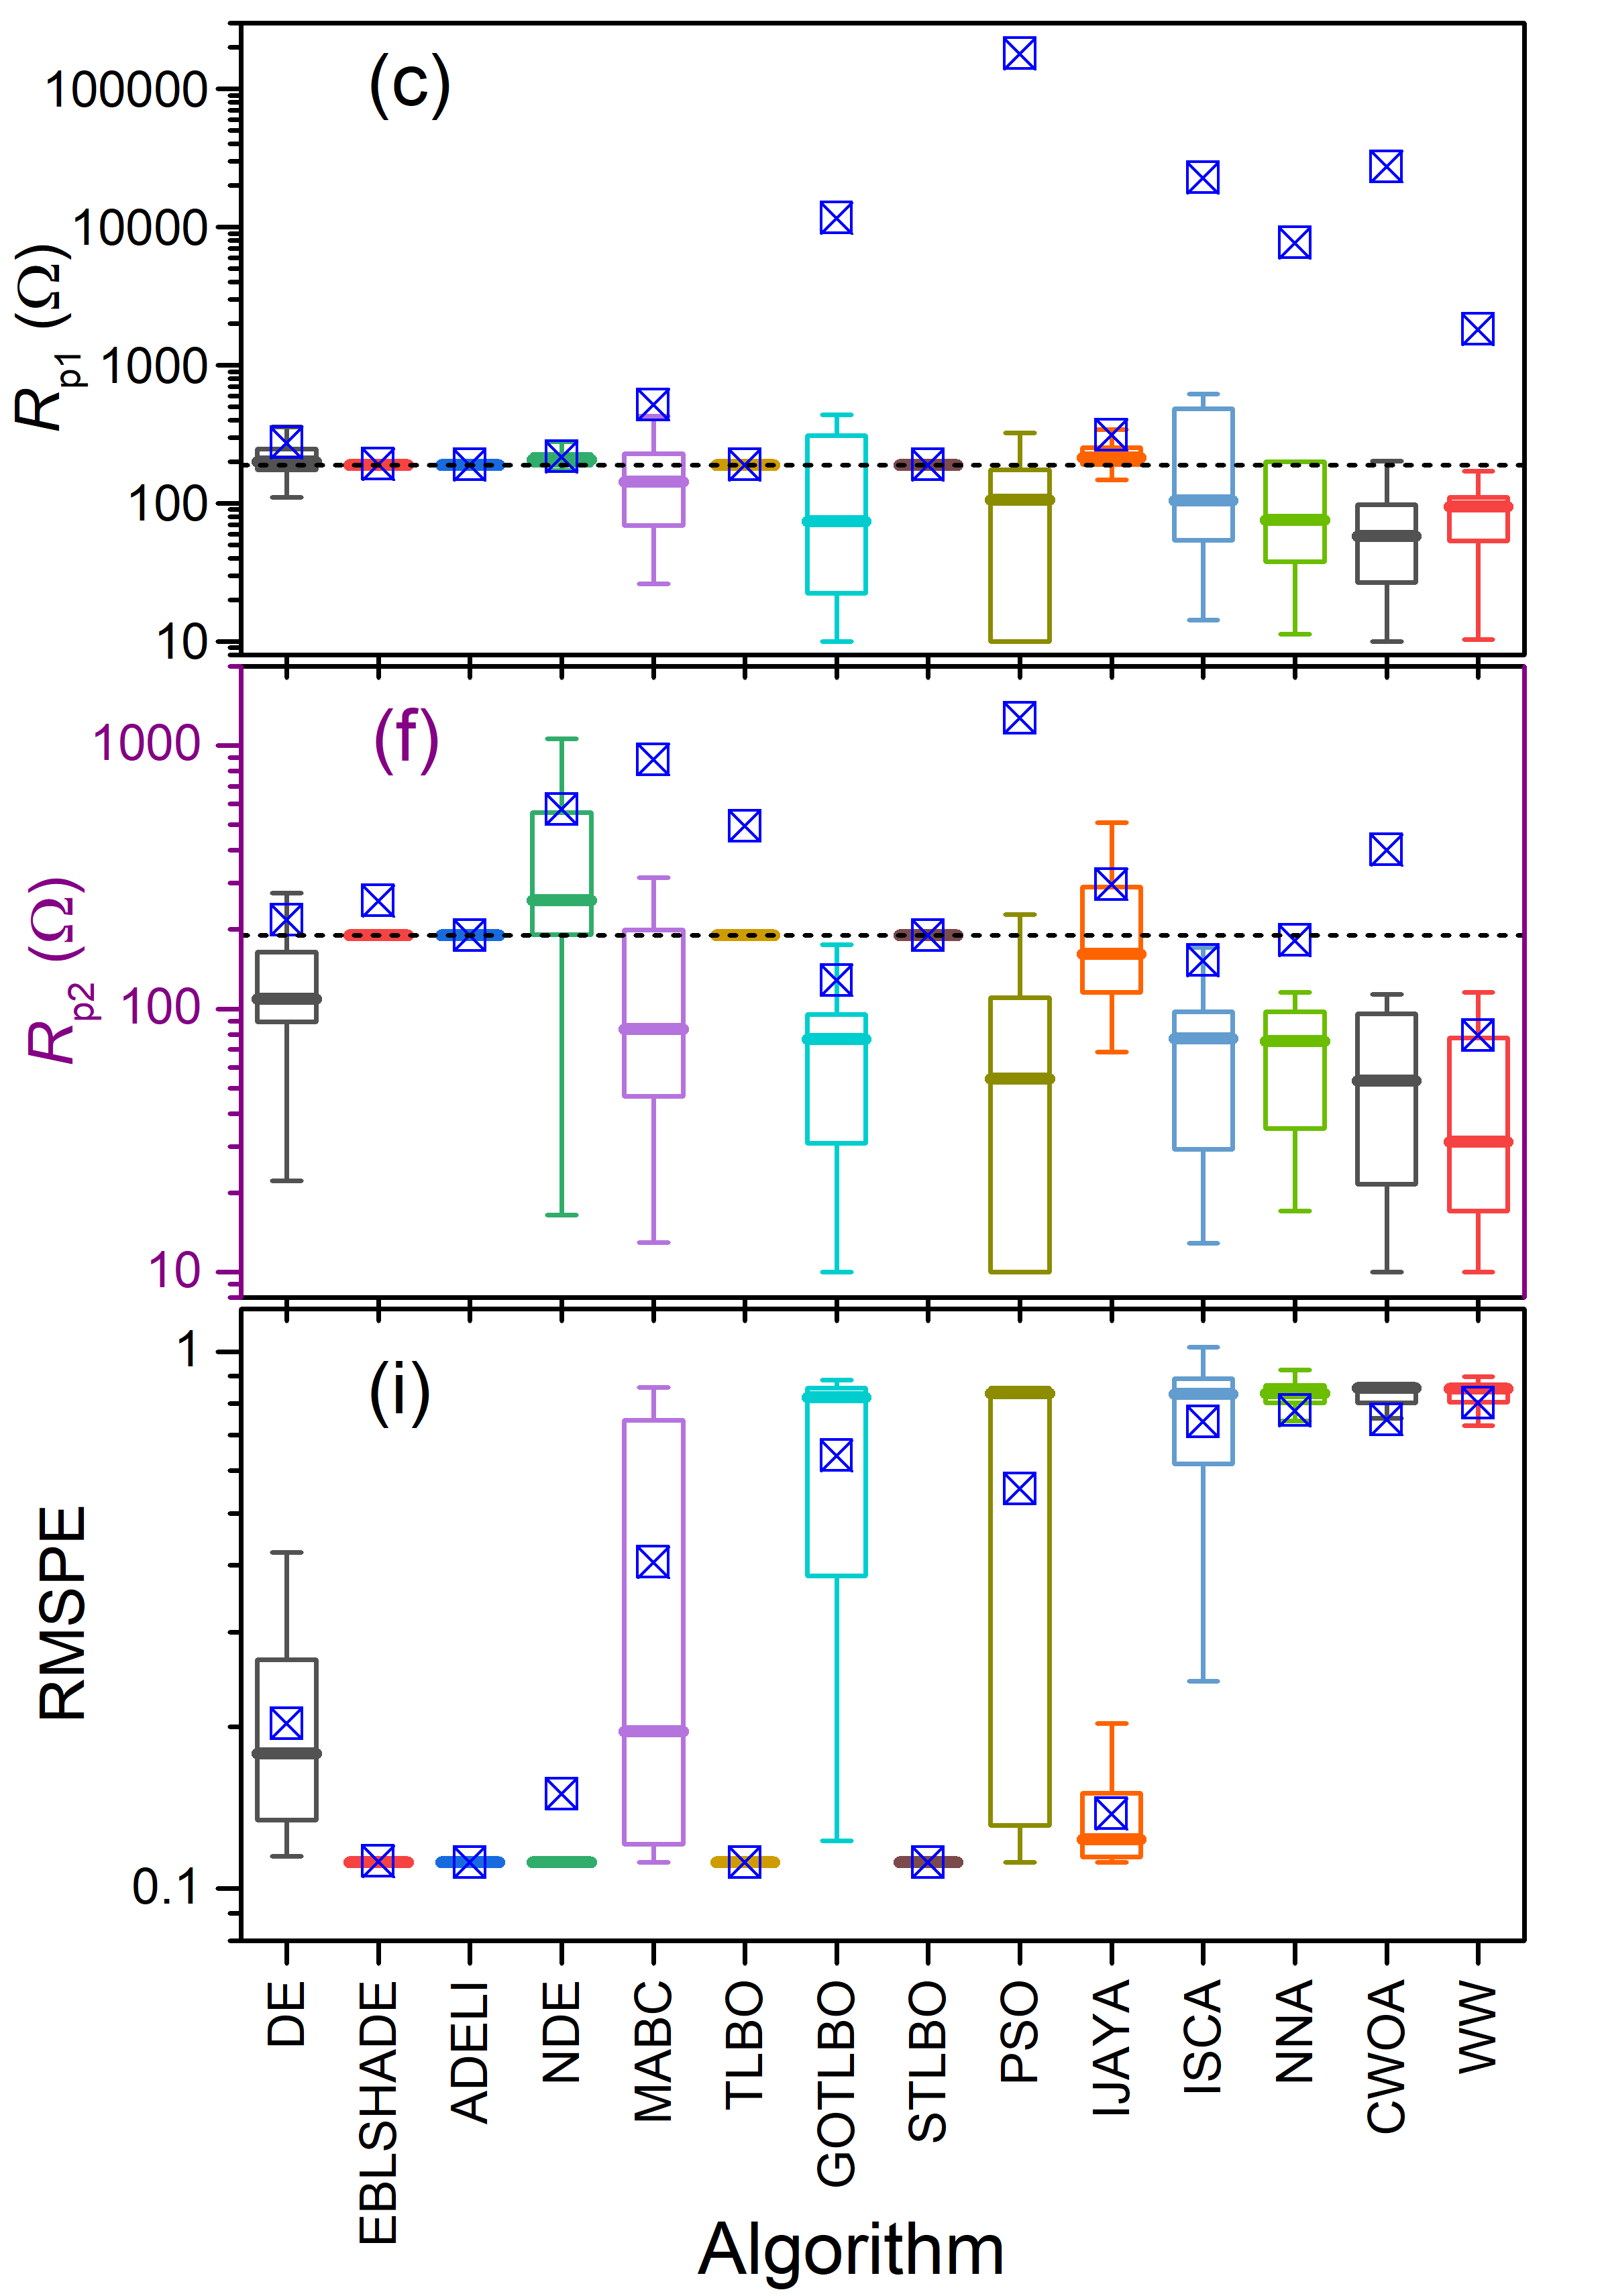
\includegraphics[width=.32\textwidth]{Fig3c}
	  \caption{Box--plot of  two--diode model parameter evaluation from single IV curve using different optimizers.
      The squares are the mean values, and the dashed lines correspond to the true parameter values.}\label{figBoxSingleIV}
\end{figure*}

We would like to stress the following.
In most cases, median values are more relevant to the actual parameter values than the mean values.
Possible exceptions only apply to the evaluation of $R_\mathrm{s}$ and $R_\mathrm{p2}$ only.
However, in cases where a method allows for parameter estimation with high accuracy (EBLSHADE, ADELI, TLBO, and STLBO),
MEDIANs are at least as good as the MEANs.
As a result, we will utilize median values as a robust measure of central tendency in nonparametric statistical tests.
Secondly, the increase in algorithm stability (reduction in STD and IQR values) in determining each model parameter correlates with the accuracy of parameter evaluation. Furthermore, IQR values are generally no worse than STD values.
Finally, small RMSPE values (close match between the fitting curve and the IV points)
do not always indicate high accuracy in determining the parameters of a solar cell --- see IJAYA and NDE data.
For example, the difference between the $\mathrm{MEDIAN}_\mathrm{RMSPE}$ values for NDE and ADELI is approximately 0.0001
(about 0.08\% of their absolute value).
At the same time, in the ADELI case, the values of $\mathrm{APE}_\mathrm{MEDIAN}$ do not exceed $6\cdot 10^{-4}$
for all model parameters evaluation,
whereas for the NDE algorithm application, the obtained $\mathrm{APE}_\mathrm{MEDIAN}$ values are significantly higher
and range from 0.04 for $I_\mathrm{ph}$ to 11.4 for $I_{01}$.
On one hand, this confirms the issue identified by Tada \cite{Tada2015Organic,Tada2021}, which arises when estimating
parameters according to the opposed two--diode model from similar IV curves corresponding to photovoltaic cells with distinct characteristics.
Furthermore, the results indicate that some metaheuristic algorithms, such as NDE and IJAYA, can fall into a similar trap.
On the other hand, the high accuracy in parameter estimation demonstrated by EBLSHADE, ADELI, and STLBO indicates
that these algorithms are able to overcome the mentioned issue when applied.
It should be noted that a similar problem has been previously addressed by employing Bayesian estimation of parameters \cite{Tada2021}.
However, each Bayesian calculation took approximately half a day on a computer better equipped than ours \cite{Tada2021}.
In our case, when applying meta--heuristic algorithms, the worst--case run time did not exceed 100 seconds.

In order to statistically compare the algorithm under consideration, we use nonparametric tests.
In the single--IV case, all nonparametric statistical tests were used to compare the performance of meta--heuristic algorithms in assessing each of the eight model parameters.
The $\mathrm{APE}_i$ values were used, and the number of case problems in the study $n$ was equal to $N_\mathrm{runs}=51$.
Additionally, algorithms were compared in terms of curve-fitting accuracy by using RMSPE values.
Furthermore, tests were employed for a composite parameter as well.
This parameter, referred to as ``Comp'' hereafter, includes $\mathrm{APE}_\mathrm{MEDIAN}$ for each of the eight defined model parameters,
the median value for RMSPE, and $t_\mathrm{run}$.
This parameter may provide the most valuable insights for comparing algorithms. However, it is important to note that the value of $n$ is only 10.
According to Derrac \emph{et al} \cite{Derrac2011}, the number of case problems should be $n\geq 2k$,
where $k$ is the number of algorithms ($k=14$ in our study).
Therefore, the use of the Comp parameter is not strictly rigorous.
Indeed, it would have been possible to increase the $n$ value using, for example, $\mathrm{APE}_\mathrm{MEAN}$.
However, considering the deliberate utilization of a suboptimal parameter would have appeared inappropriate.



\begin{figure}[]
	\centering
		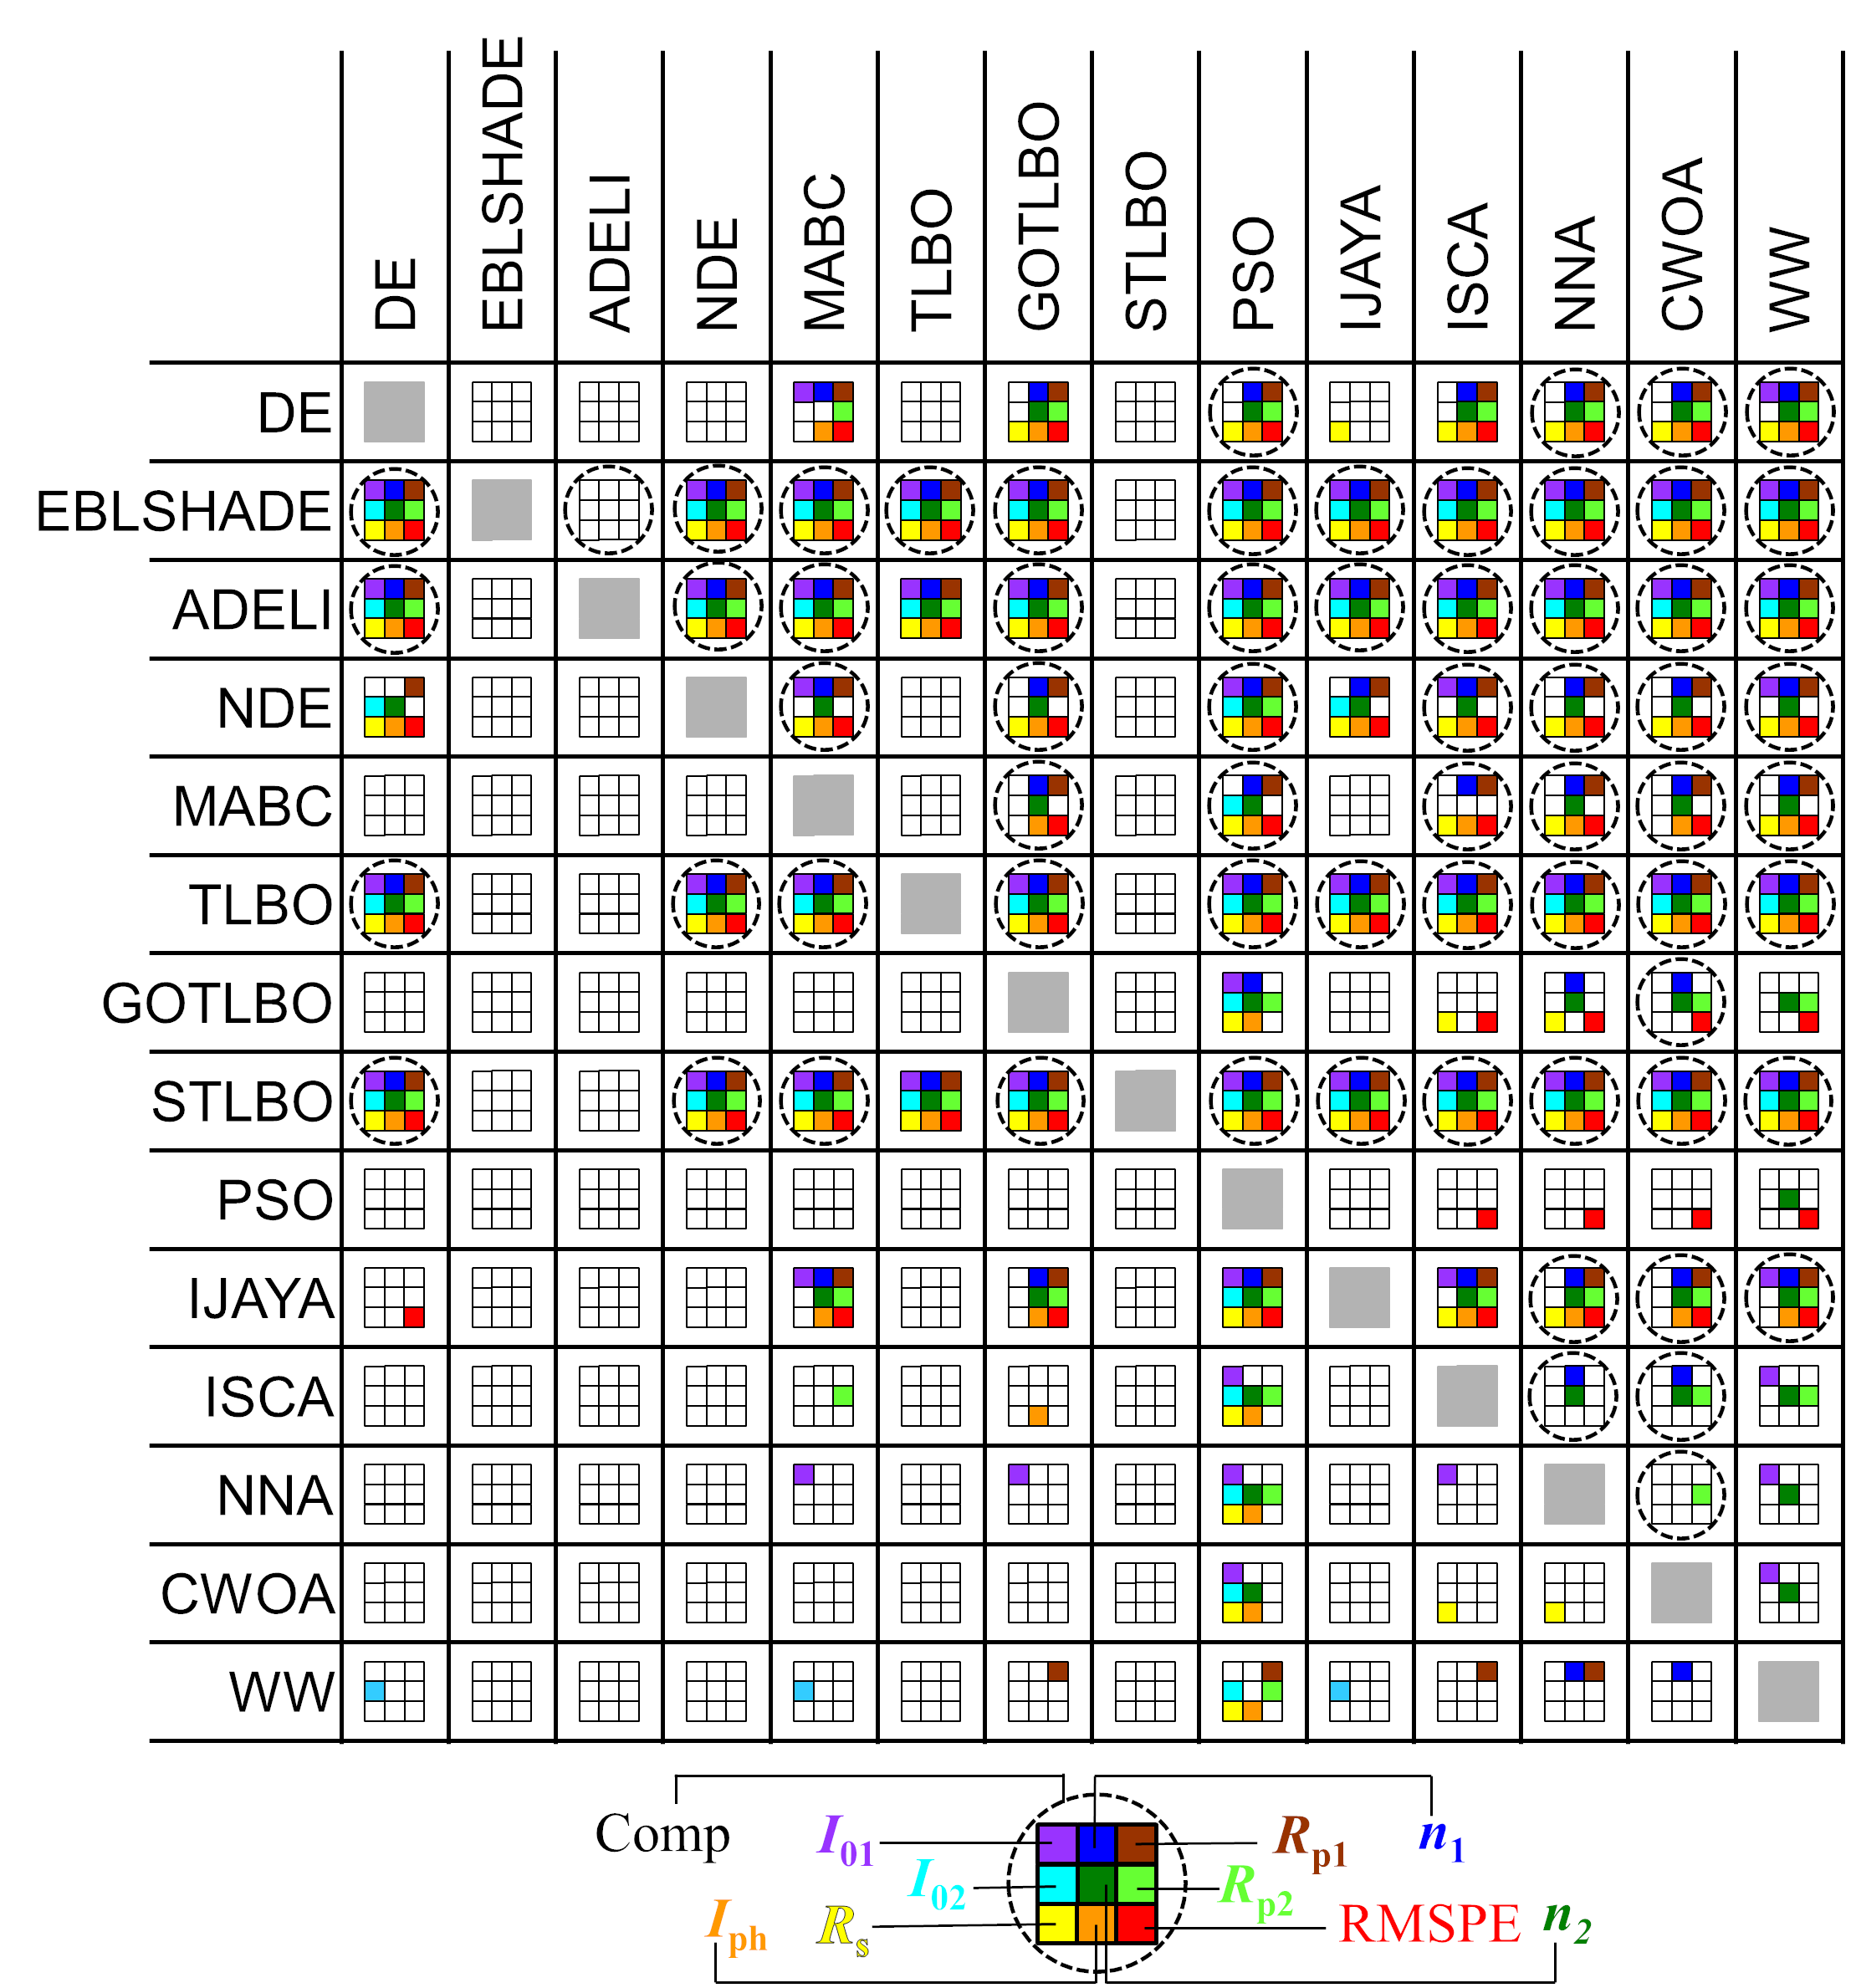
\includegraphics[width=1.0\columnwidth]{Fig4}
	  \caption{The results of Wilcoxon signed-rank test with a level of significance $\alpha = 0.05$ in the single-IV case.
               Each colored small square indicates that the algorithm specified in the row outperforms the algorithm
               specified in the column in evaluating one of the parameters of the two--diode model.
               The correspondence between the color and position of the square to a model parameter
               is shown in a legend at the figure bottom.
               The advantage of the row algorithm in the Comp parameter is indicated by the presence of a dashed circle.}\label{figWilSingleIV}
\end{figure}

\begin{figure}[]
	\centering
		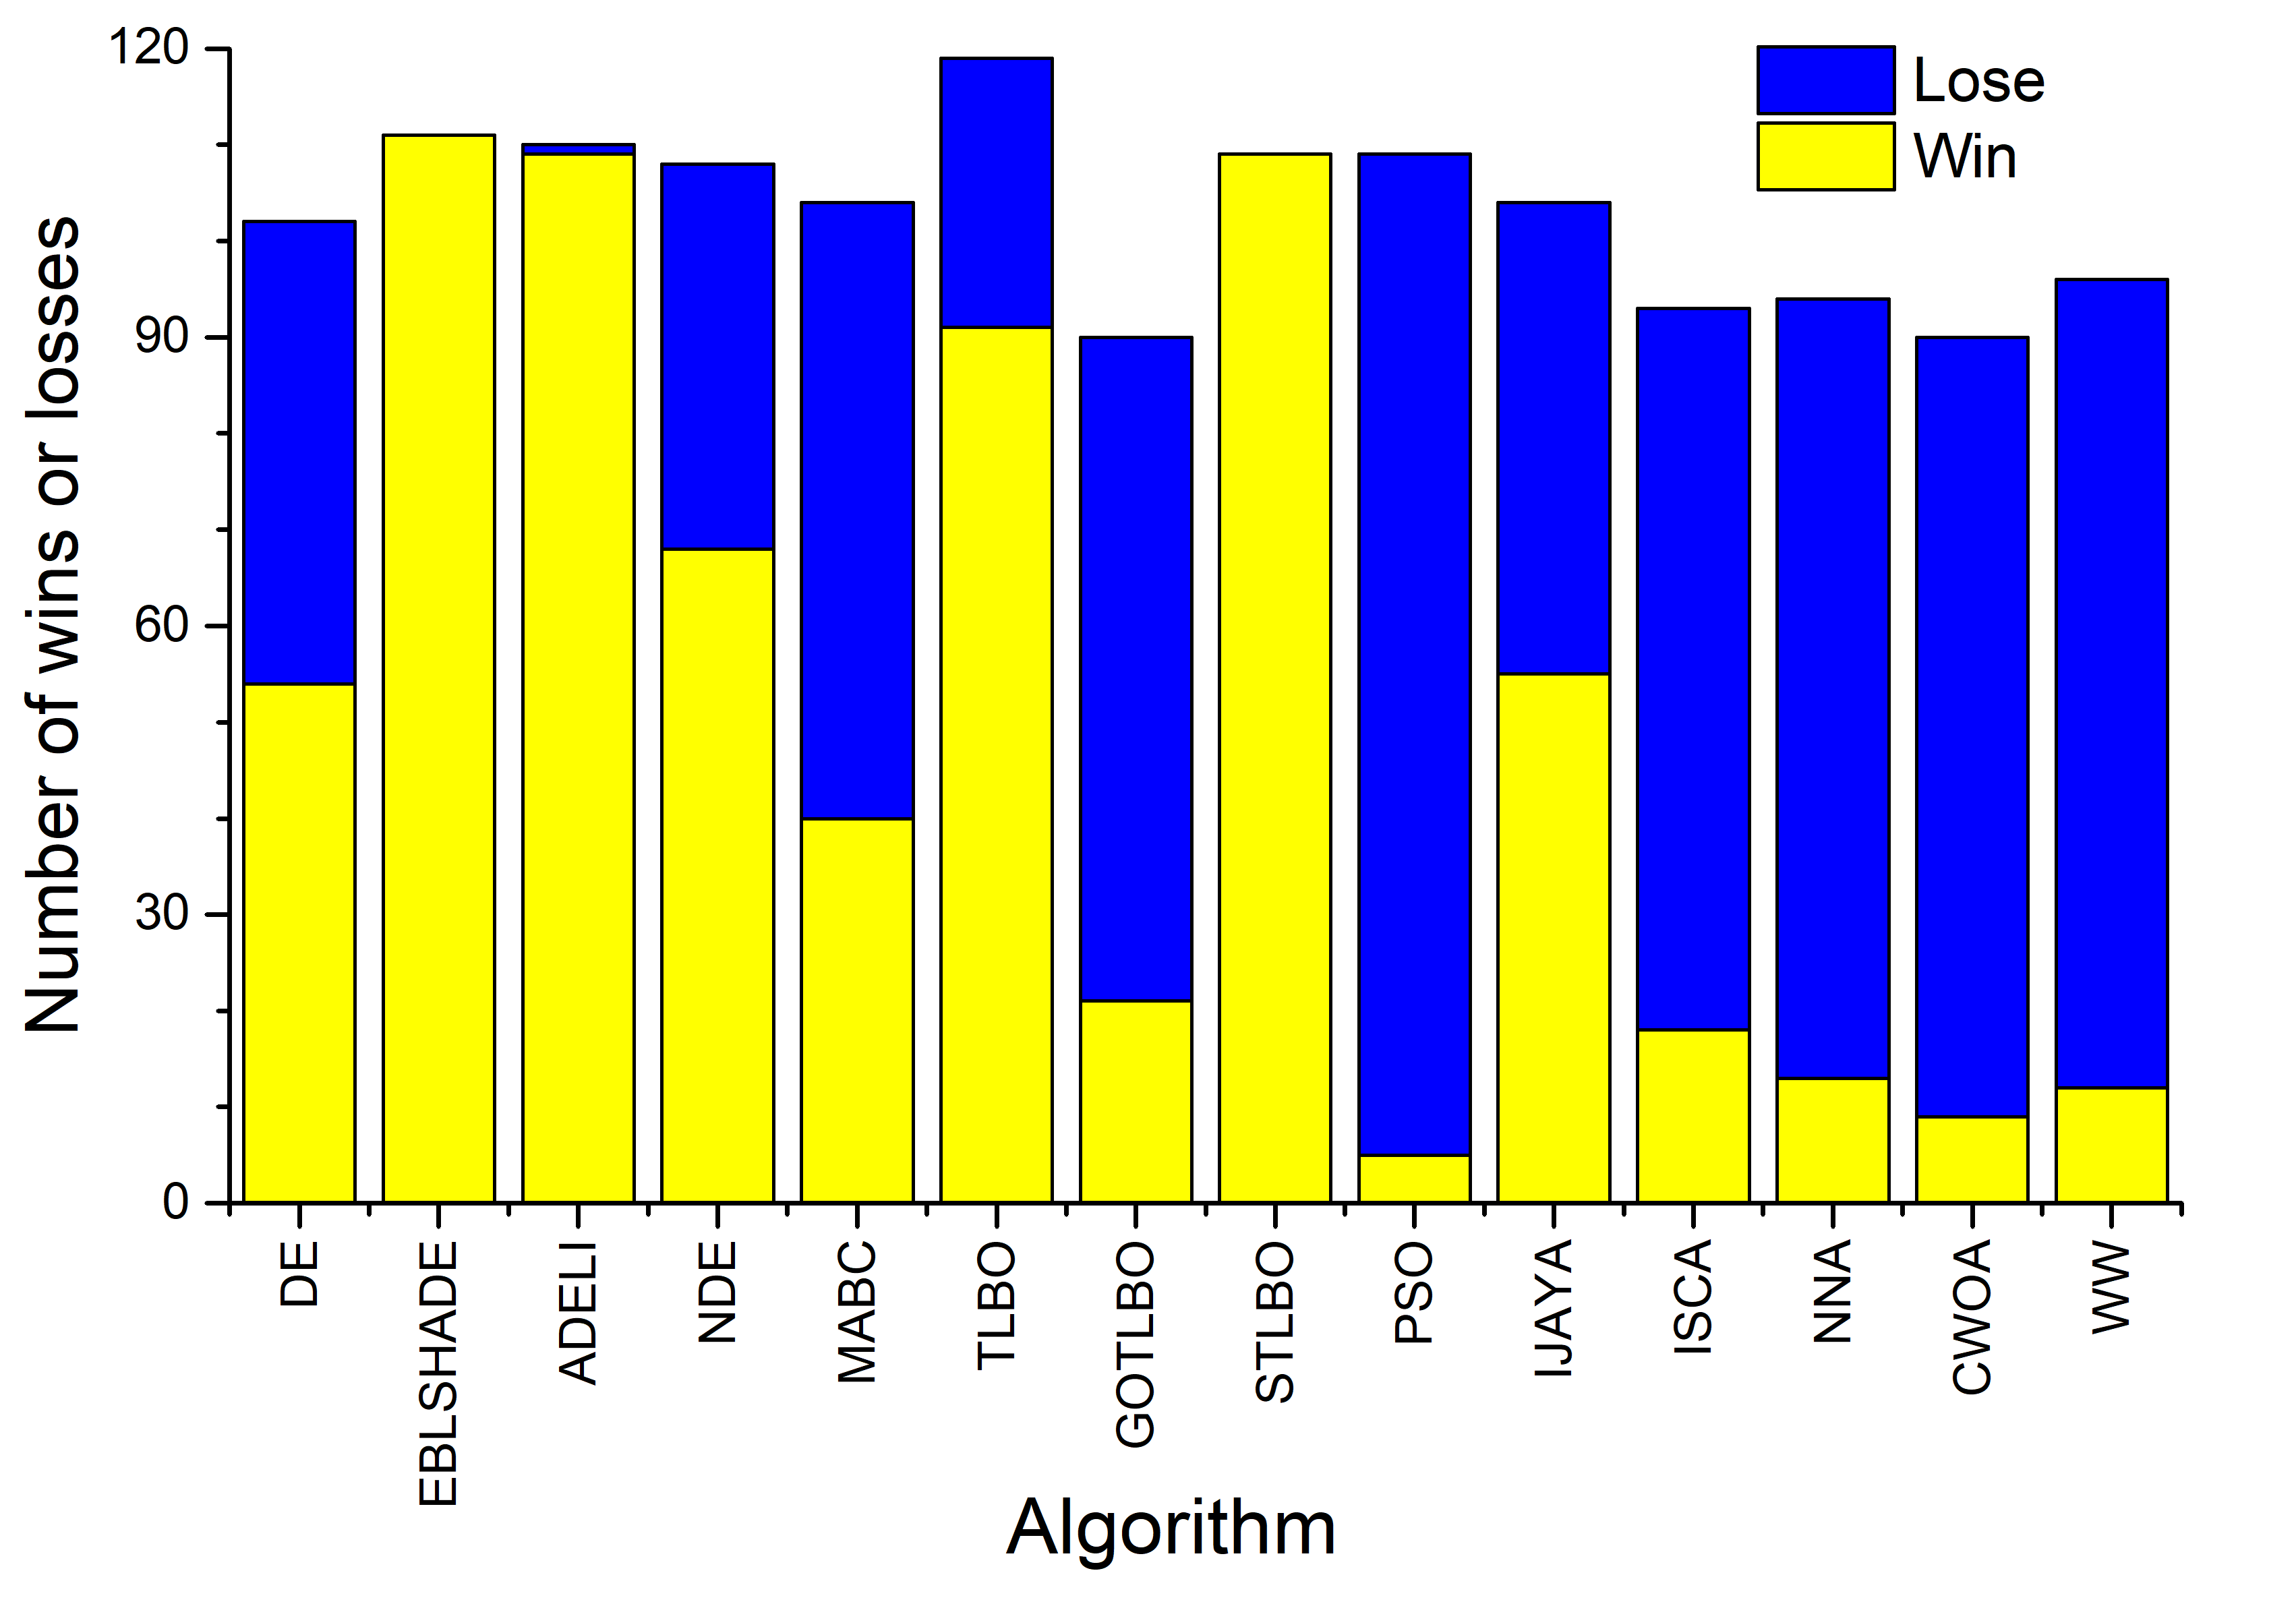
\includegraphics[width=1.0\columnwidth]{Fig5}
	  \caption{The total number of wins and losses for each algorithm in pairwise comparisons using the
               Wilcoxon signed-rank test with a significance level of $\alpha = 0.05$ in the single-IV case.}\label{figWilTotSingleIV}
\end{figure}




Fig.~\ref{figWilSingleIV} graphically show
the non--parametric statistical results of pairwise comparisons of algorithms
based on the Wilcoxon signed--rank test.
In the case of Comp comparisons, the differences in performance scores
were normalized to the interval $[0,\, 1]$.
As seen from the figure, no algorithm outperforms all others in evaluating each parameter.
Furthermore, no algorithm surpasses all others in the evaluation even a single parameter.
For example, as the figure states, STLBO shows a significant improvement over
DE, NDE, MABC, GOTLBO, PSO, IJAYA, ISCA, NNA, CWOA, and WW across all the parameters considered
with a level of significance $\alpha = 0.05$.
Simultaneously, it was not detected the significant differences
between STLBO and both EBLSHADE and ADELI for all parameter evaluations
as well as between STLBO and TLBO in the Comp case.
EBLSHADE outperforms nearly all other algorithms in the composite parameter, except for STLBO.
According to the Wilcoxon test victories number,
the worst performances are exhibited by PSO and CWOA.
PSO achieved better results than ISCA, NNA, and CWOA in terms of RMSPE value,
as well as outperformed WW in $n_2$ evaluation and RMSPE.
Test detected significant differences between CWOA and WW in $n_2$ and $I_{01}$ evaluations,
between CWOA and PSO in $I_{01}$, $I_{02}$, $R_\mathrm{s}$, and $I_\mathrm{ph}$ evaluations),
and between CWOA and both ISCA and NNA in $R_\mathrm{s}$  evaluation case only.


Looking at the results of the Wilcoxon signed-rank test from another perspective,
it can be observed that neither EBLSHADE nor STLBO had any defeats in pairwise comparisons,
while ADELI had only one loss.
ADELI was only outperformed by EBLSHADE in terms of the Comp parameter, primarily due to its significantly longer run time.
The highest number of defeats was observed for the PSO and WW algorithms (104 and 84, respectively).
The data regarding the total number of wins and losses when applying the Wilcoxon test
for each algorithm are summarized in Fig.~\ref{figWilTotSingleIV}.

\begin{figure}[!ht]
	\centering
		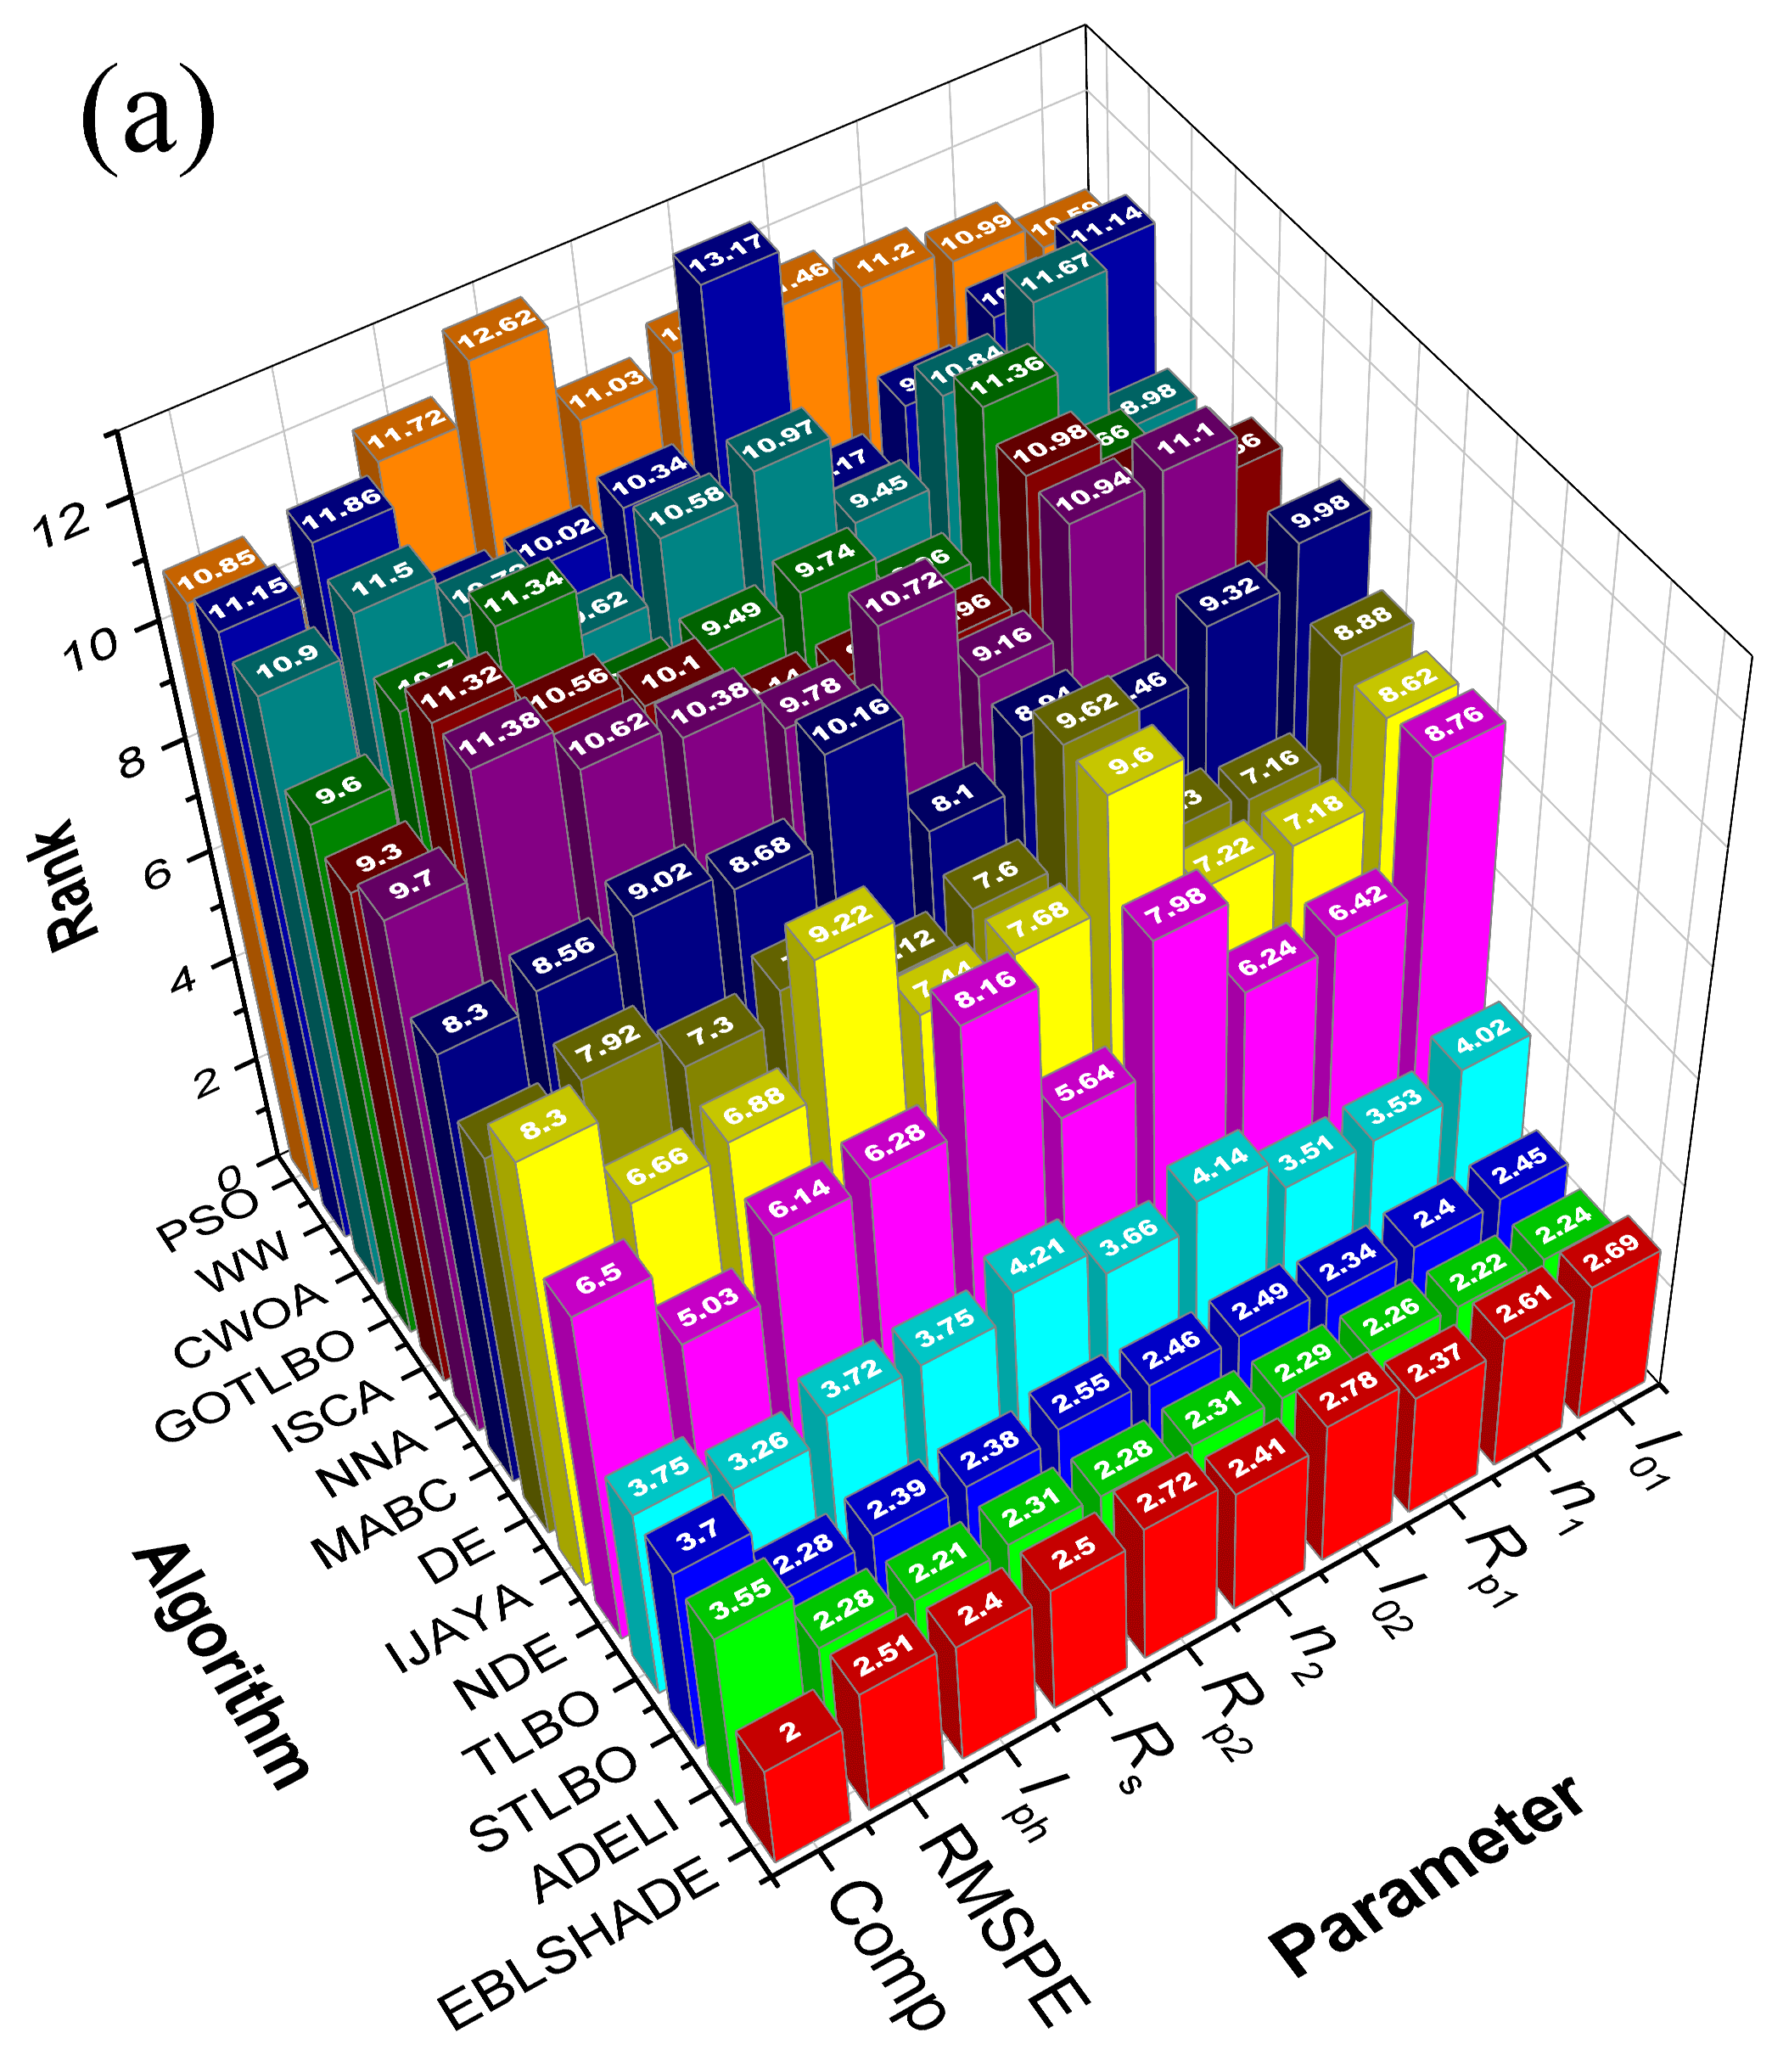
\includegraphics[width=.76\columnwidth]{Friedman}
        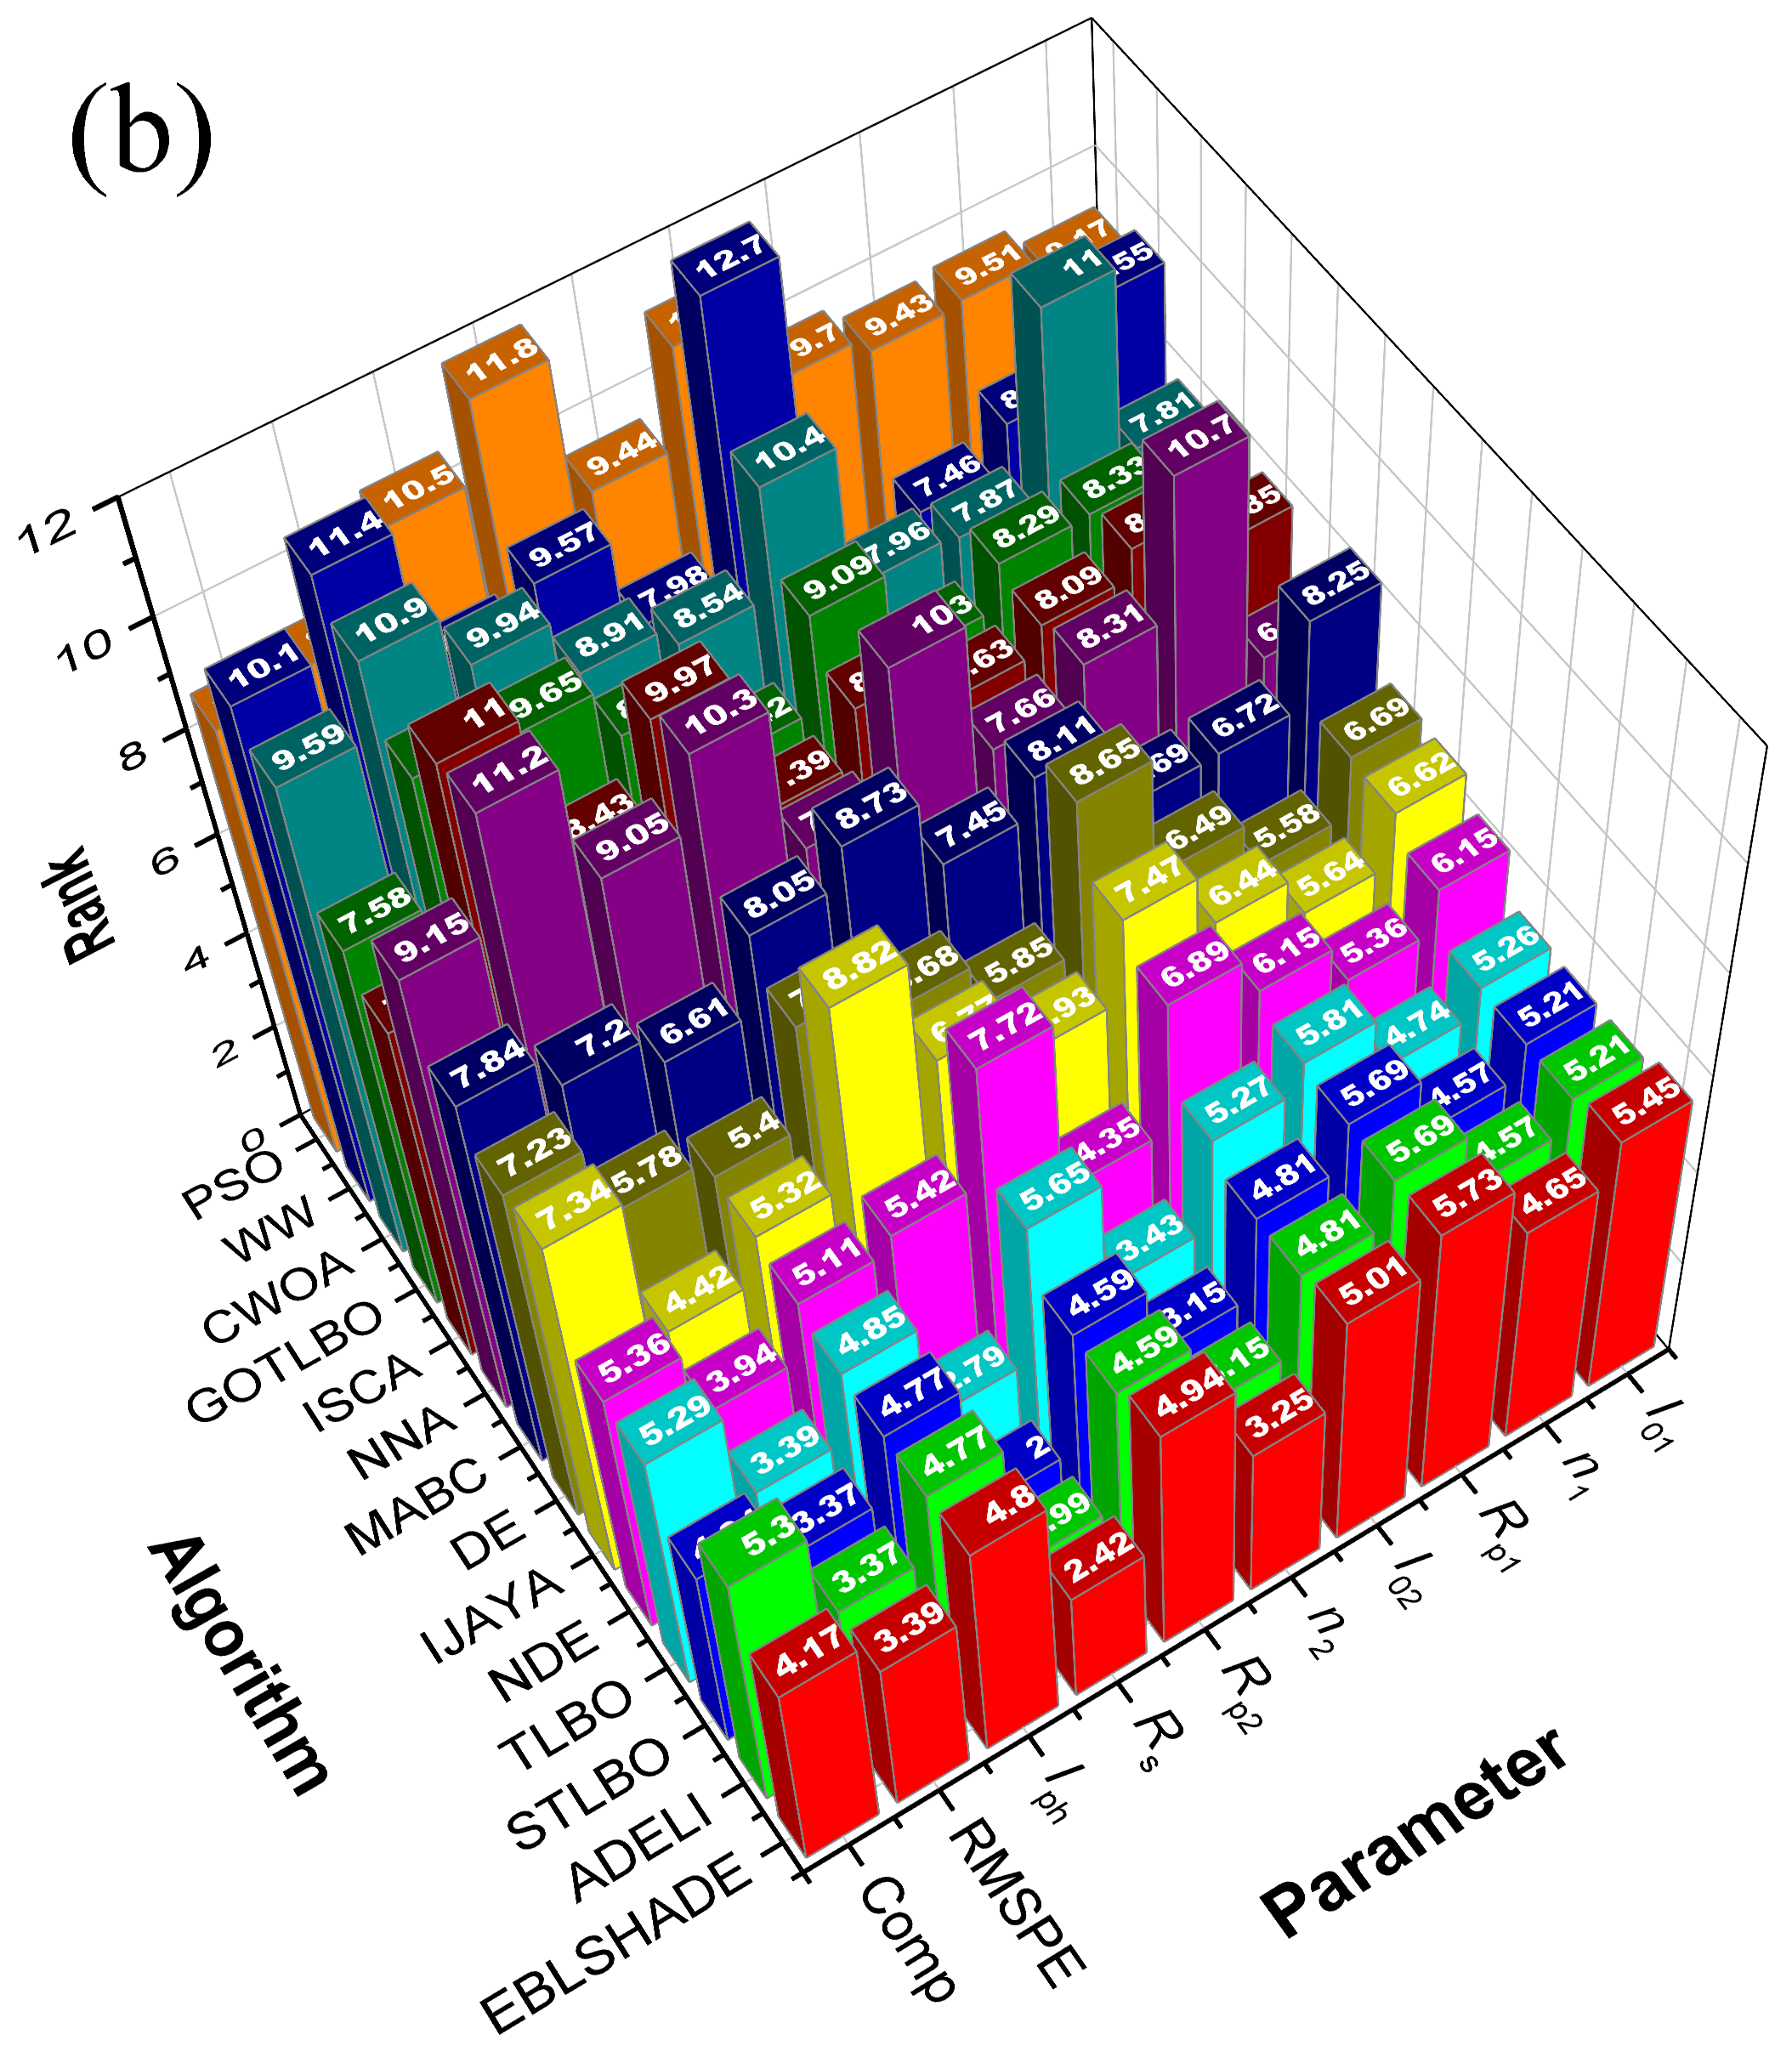
\includegraphics[width=.76\columnwidth]{FriedmanAlignedRank}
        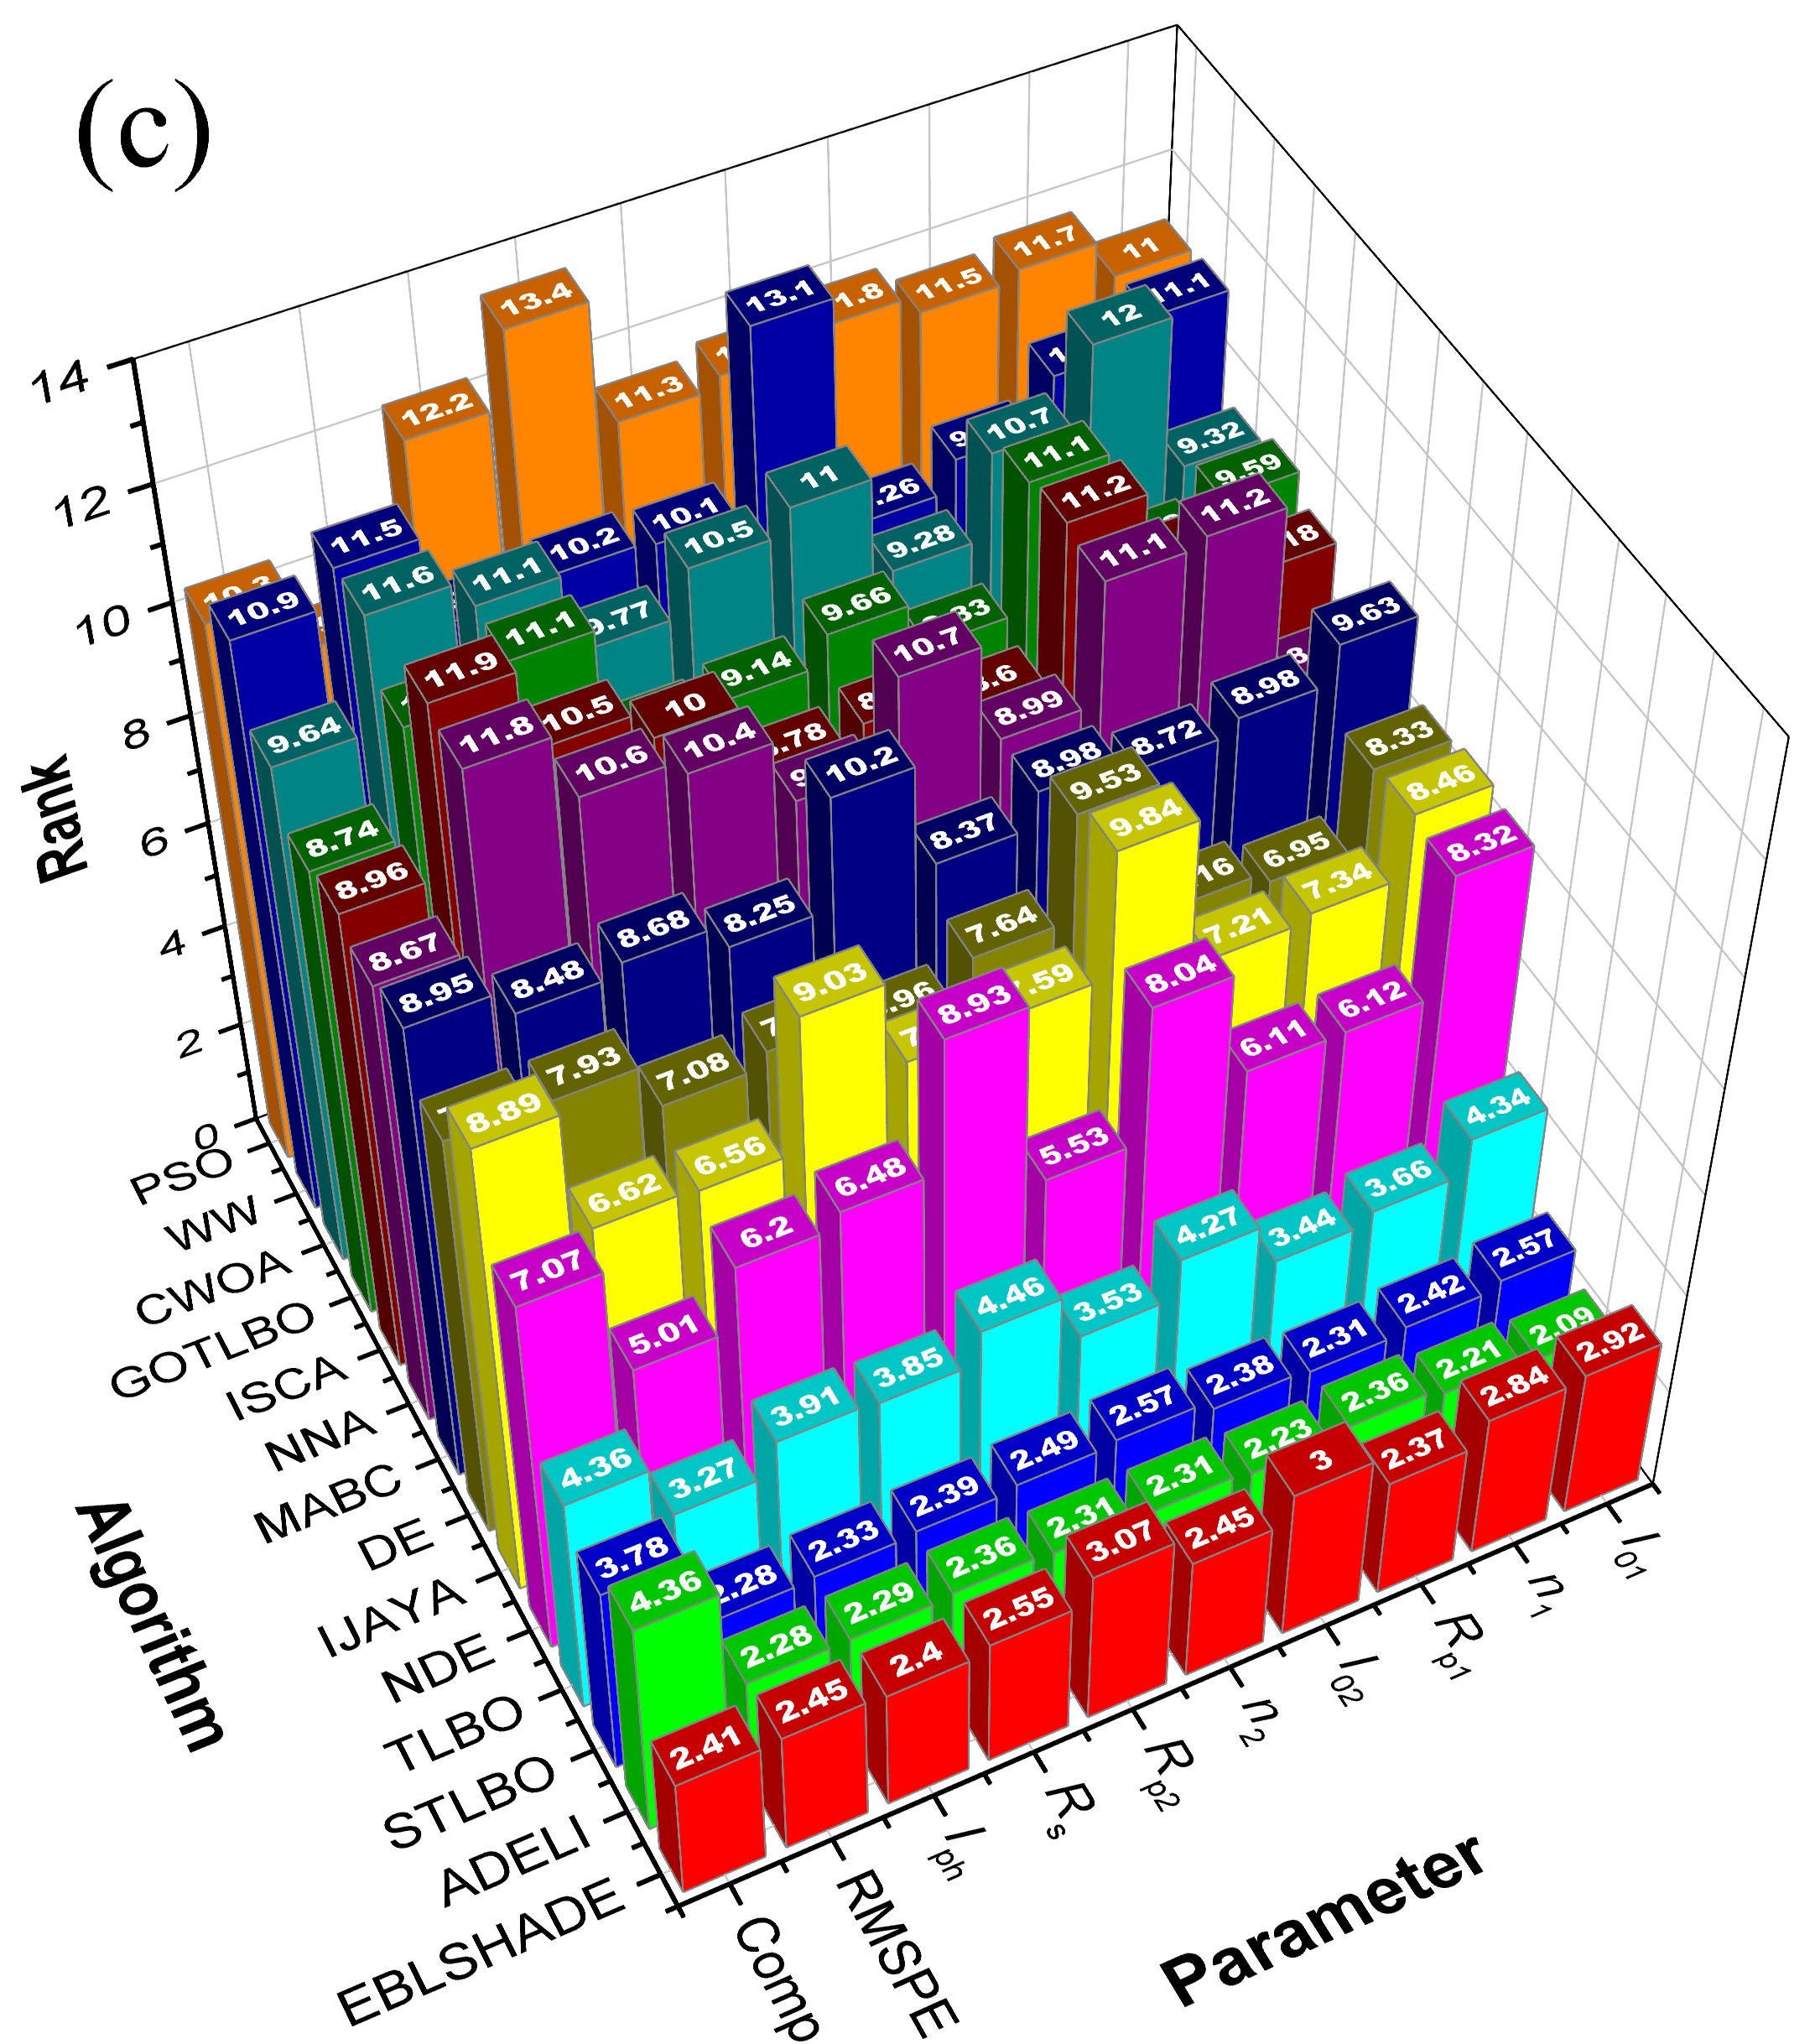
\includegraphics[width=.76\columnwidth]{QuadeRank}
	  \caption{Ranking of the algorithms according to Friedman (a), Friedman Aligned (b), and Quade (c) tests in the single-IV case.}\label{figRanksSingleIV}
\end{figure}

It is recommended \cite{Derrac2011} to begin the multiple comparison tests by examining the null hypothesis $H_0$,
which asserts the equality of medians between the populations of results obtained by different algorithms.
The null hypothesis $p$--values computed through the statistics of  Friedman, Friedman Aligned, and Quade test
and the Iman–Davenport extension
are given in the supplementary material (table S2).
The highest observed $p(H_0)$--values were found to be $2.7\cdot10^{-5}$ (Friedman Aligned test for the task of $R_\mathrm{p1}$ evaluation),
$4.4\cdot10^{-4}$ (Friedman Aligned test for the composite parameter case),
and $8.3\cdot10^{-6}$ (Quade test, Comp parameter).
Thus obtained data strongly suggest the existence of significant differences
among the considered algorithms in the accuracy of all model parameter determination, RMSPE values, and Comp parameter.



Fig.~\ref{figRanksSingleIV} shows
ranks achieved by the Friedman, Friedman Aligned, and Quade tests for applied optimization algorithms in different tasks.
Ranks are tabulated in the supplementary material as well (table S3).
In almost all cases, the algorithms EBLSHADE, ADELI, and STLBO consistently achieve the top (smallest value) three ranks.
For example, in assessing the accuracy of model parameter evaluation, ADELI has ranked first 22 times.
The STLBO algorithm ranked first six times,
taking the sole first place twice ($I_{01}$ evaluation according Friedman Aligned test and
$R_\mathrm{p1}$ evaluation according Quade test)
and sharing it with ADELI four times ($n_1$, $R_\mathrm{p1}$, $n_2$, and $I_\mathrm{ph}$ evaluation according Friedman Aligned test).
In the RMSPE value case, ADELI and STLBO achieved equal and best ranks by all three used tests.
When comparing based on the Comp parameter,
the STLBO algorithm obtained the top rank according to the Friedman Aligned test,
while the Friedman and Quade tests recognized EBLSHADE as the best.
In most cases, the TLBO algorithm secured the fourth position, and in four cases, it even ranked third.
In the majority of cases, the TLBO algorithm consistently ranked fourth out of all the algorithms tested.
Interestingly, in four cases ($I_{01}$ evaluation, RMSPE value, and Comp parameter by Friedman Aligned test,
and Comp parameter by Quade test),
it even achieved a commendable third-place ranking.
We must note that overall, the absolute values of ranks for ADELI, STLBO, EBLSHADE and TLBO algorithms differ little,
and the difference between the first and fourth ranks is often less than 0.5.
The worst ranks are observed for PSO, NNA, CWOA, and WW.

It is known \cite{Derrac2011} that
the Friedman, Friedman Aligned, and Quade tests are insufficient in establishing accurate comparisons between the algorithms considered.
To compare a control method (1 of 14 compared) with a set of other algorithms (rest 13),
one can define a family of hypotheses related to the control method.
Applying a post-hoc test makes it possible to obtain a $p$--value that indicates the extent to which each hypothesis can be rejected.
We calculated $p$--values using four post-hoc procedures (Finner, Holm, Hochberg, and Holland) for all algorithms, tests, and tasks.
By following the indications given for the four post-hoc procedures considered, Table~\ref{tbl1NADELI} shows the $p$--values
obtained, using the ranks computed by the Friedman, Friedman Aligned, and Quade tests for the case of control algorithm ADELI
and the task of $R_\mathrm{p1}$ evaluation.
These are typical results, the reader is referred to the supplementary material for rest of $p$-values (Tables S4-S143).


\begin{table*}[<options>]
\caption{Adjusted $p$-values for Friedman, Friedman Aligned, and Quade tests in single--IV case.
 ADELI is the control algorithm, and the task of $R_\mathrm{p1}$ evaluation is under consideration.}\label{tbl1NADELI}
\begin{tabular*}{\tblwidth}{@{}LLCCCC@{}}
\toprule
\multirow{2}{*}{Algorithm}& \multirow{2}{*}{Test}& \multicolumn{4}{C}{post-hoc procedure} \\
  & &Finner & Holm & Hochberg &Holland\\ % Table header row
\midrule
GOTLBO&	Friedman&<1E-13&<1E-13&<1E-13&<1E-13\\
&Friedman Aligned&2.23361E-09&6.87266E-09&6.87266E-09&6.87266E-09\\
&Quade&2.57827E-03&4.09880E-03&3.90245E-03&4.09117E-03\\
PSO&Friedman&<1E-13&<1E-13&<1E-13&<1E-13\\
&Friedman Aligned&<1E-13&<1E-13&<1E-13&<1E-13\\
&Quade&2.57827E-03&2.58134E-03&2.58134E-03&2.57827E-03\\
MABC&Friedman&6.35048E-13&1.61204E-12&1.61204E-12&1.61204E-12\\
&Friedman Aligned&7.88131E-06&2.97065E-05&2.97065E-05&2.97062E-05\\
&Quade&1.73550E-02&6.56791E-02&6.56791E-02&6.38590E-02\\
WW&Friedman&1.84926E-10&5.69003E-10&5.69003E-10&5.69003E-10\\
&Friedman Aligned&3.15599E-13&8.01137E-13&8.01137E-13&8.01137E-13\\
&Quade&5.31725E-03&1.96611E-02&1.96611E-02&1.94928E-02\\
DE&Friedman&4.61292E-09&1.59678E-08&1.59678E-08&1.59678E-08\\
&Friedman Aligned&3.62181E-04&1.33738E-03&1.33738E-03&1.33663E-03\\
&Quade&7.62673E-02&2.85885E-01&2.49968E-01&2.53918E-01\\
IJAYA&Friedman&6.88175E-09&2.54096E-08&2.54096E-08&2.54096E-08\\
&Friedman Aligned&8.79672E-04&3.04543E-03&3.04543E-03&3.04172E-03\\
&Quade&7.62673E-02&2.85885E-01&2.49968E-01&2.53918E-01\\
CWOA&Friedman&8.73483E-09&3.29236E-08&3.29236E-08&3.29236E-08\\
&Friedman Aligned&4.27917E-09&1.58000E-08&1.58000E-08&1.58000E-08\\
&Quade&2.57827E-03&5.93402E-03&5.93402E-03&5.91840E-03\\
NNA&Friedman&1.17491E-08&4.33811E-08&4.27586E-08&4.33811E-08\\
&Friedman Aligned&2.23361E-09&7.25937E-09&7.25937E-09&7.25937E-09\\
&Quade&2.57827E-03&4.09880E-03&3.90245E-03&4.09117E-03\\
ISCA&Friedman&1.23525E-08&4.33811E-08&4.27586E-08&4.33811E-08\\
&Friedman Aligned&<1E-13&<1E-13&<1E-13&<1E-13\\
&Quade&2.57827E-03&3.65691E-03&3.65691E-03&3.65079E-03\\
NDE&Friedman&2.55436E-06&7.85957E-06&7.85957E-06&7.85955E-06\\
&Friedman Aligned&4.19953E-02&1.29854E-01&1.29854E-01&1.23666E-01\\
&Quade&1.60056E-01&5.02233E-01&5.02233E-01&4.15313E-01\\
TLBO&Friedman&1.57702E-01&4.05499E-01&4.05499E-01&3.53159E-01\\
&Friedman Aligned&6.48054E-01&1.0&1.0&9.29409E-01\\
&Quade&7.18467E-01&1.0&1.0&9.59945E-01\\
EBLSHADE&Friedman&9.13338E-01&1.0&9.23824E-01&9.89059E-01\\
&Friedman Aligned&8.67482E-01&1.0&1.0&9.76034E-01\\
&Quade&9.98363E-01&1.0&1.0&9.99993E-01\\
STLBO&Friedman&9.23824E-01&1.0&9.23824E-01&9.89059E-01\\
&Friedman Aligned&1.0&1.0&1.0&1.0\\
&Quade&1.0&1.0&1.0&1.0\\
\bottomrule
\end{tabular*}
\end{table*}


As we can see in the table, the Finner post-hoc procedure exhibits the most powerful behavior,
reaching the lowest $p$-values in the comparisons.
The Friedman test shows a significant improvement in $R_\mathrm{p1}$ evaluation of ADELI over
DE, NDE, MABC, GOTLBO, PSO, IJAYA, ISCA, NNA, CWOA, and WW
for all the post-hoc procedures considered.

The Friedman Aligned test only confirms the improvement of ADELI
over the aforementioned 10 algorithms for every post-hoc procedure considered,
except Holm, Hochberg, and Holland,
which fail to highlight the differences between ADELI and NDE as significant.

Finally, the Quade test find significant difference between ADELI and
MABC, GOTLBO, PSO, ISCA, NNA, CWOA, WW for every post-hoc procedure.
In the DE and IJAYA cases, ADELI obtains better results in $R_\mathrm{p1}$ evaluation
according Finner post-hoc procedure only.
This result supports the conclusion that,
although ADELI outperforms the weaker algorithms of our study,
its performance differences are not significant when compared to other power algorithms (STLBO, EBLSHADE, TLBO).

In our study, a threshold value of $p_{lim}=0.1$ was adopted to establish a limit level
for comparing the effectiveness of two algorithms in both multiple $1\times N$ and $N\times N$ comparisons.
That is, it was determined that the likelihood of obtaining a result as extreme as the observed one,
under the assumption that there is no difference between the two algorithms (null hypothesis), was less than 10\%.



\begin{figure*}[]
	\centering
		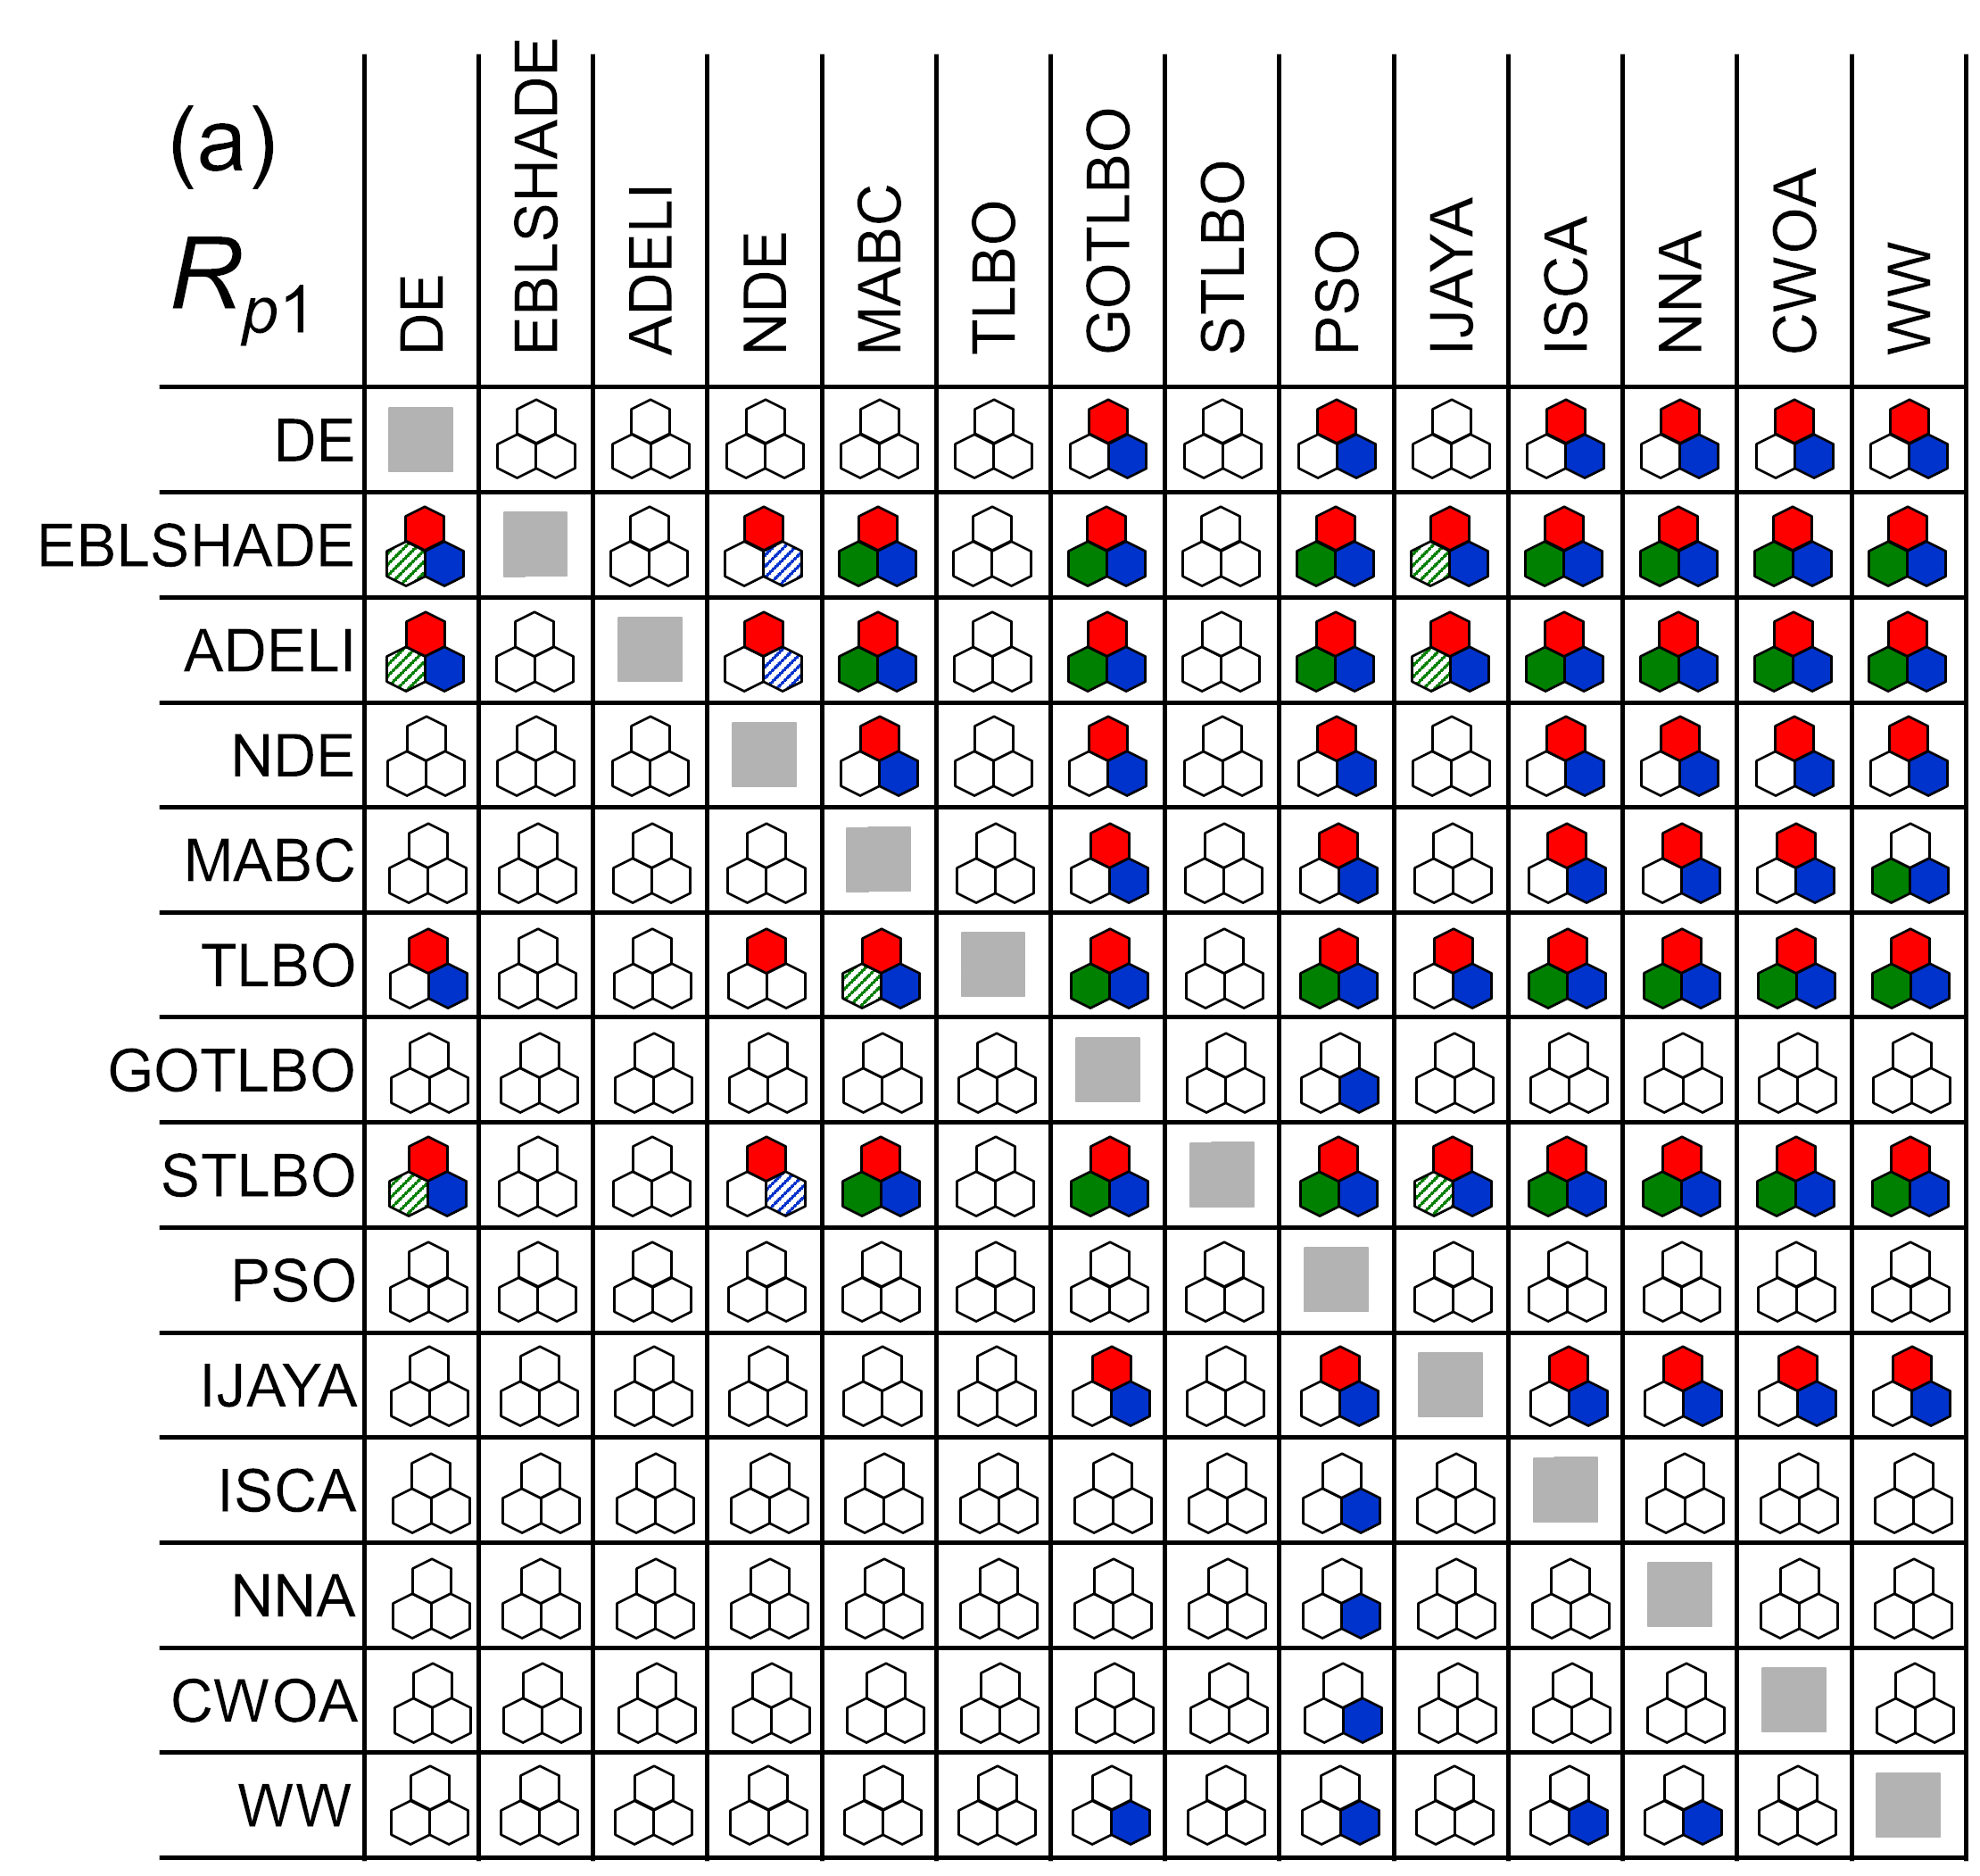
\includegraphics[width=.49\textwidth]{Rp1shotN1}
        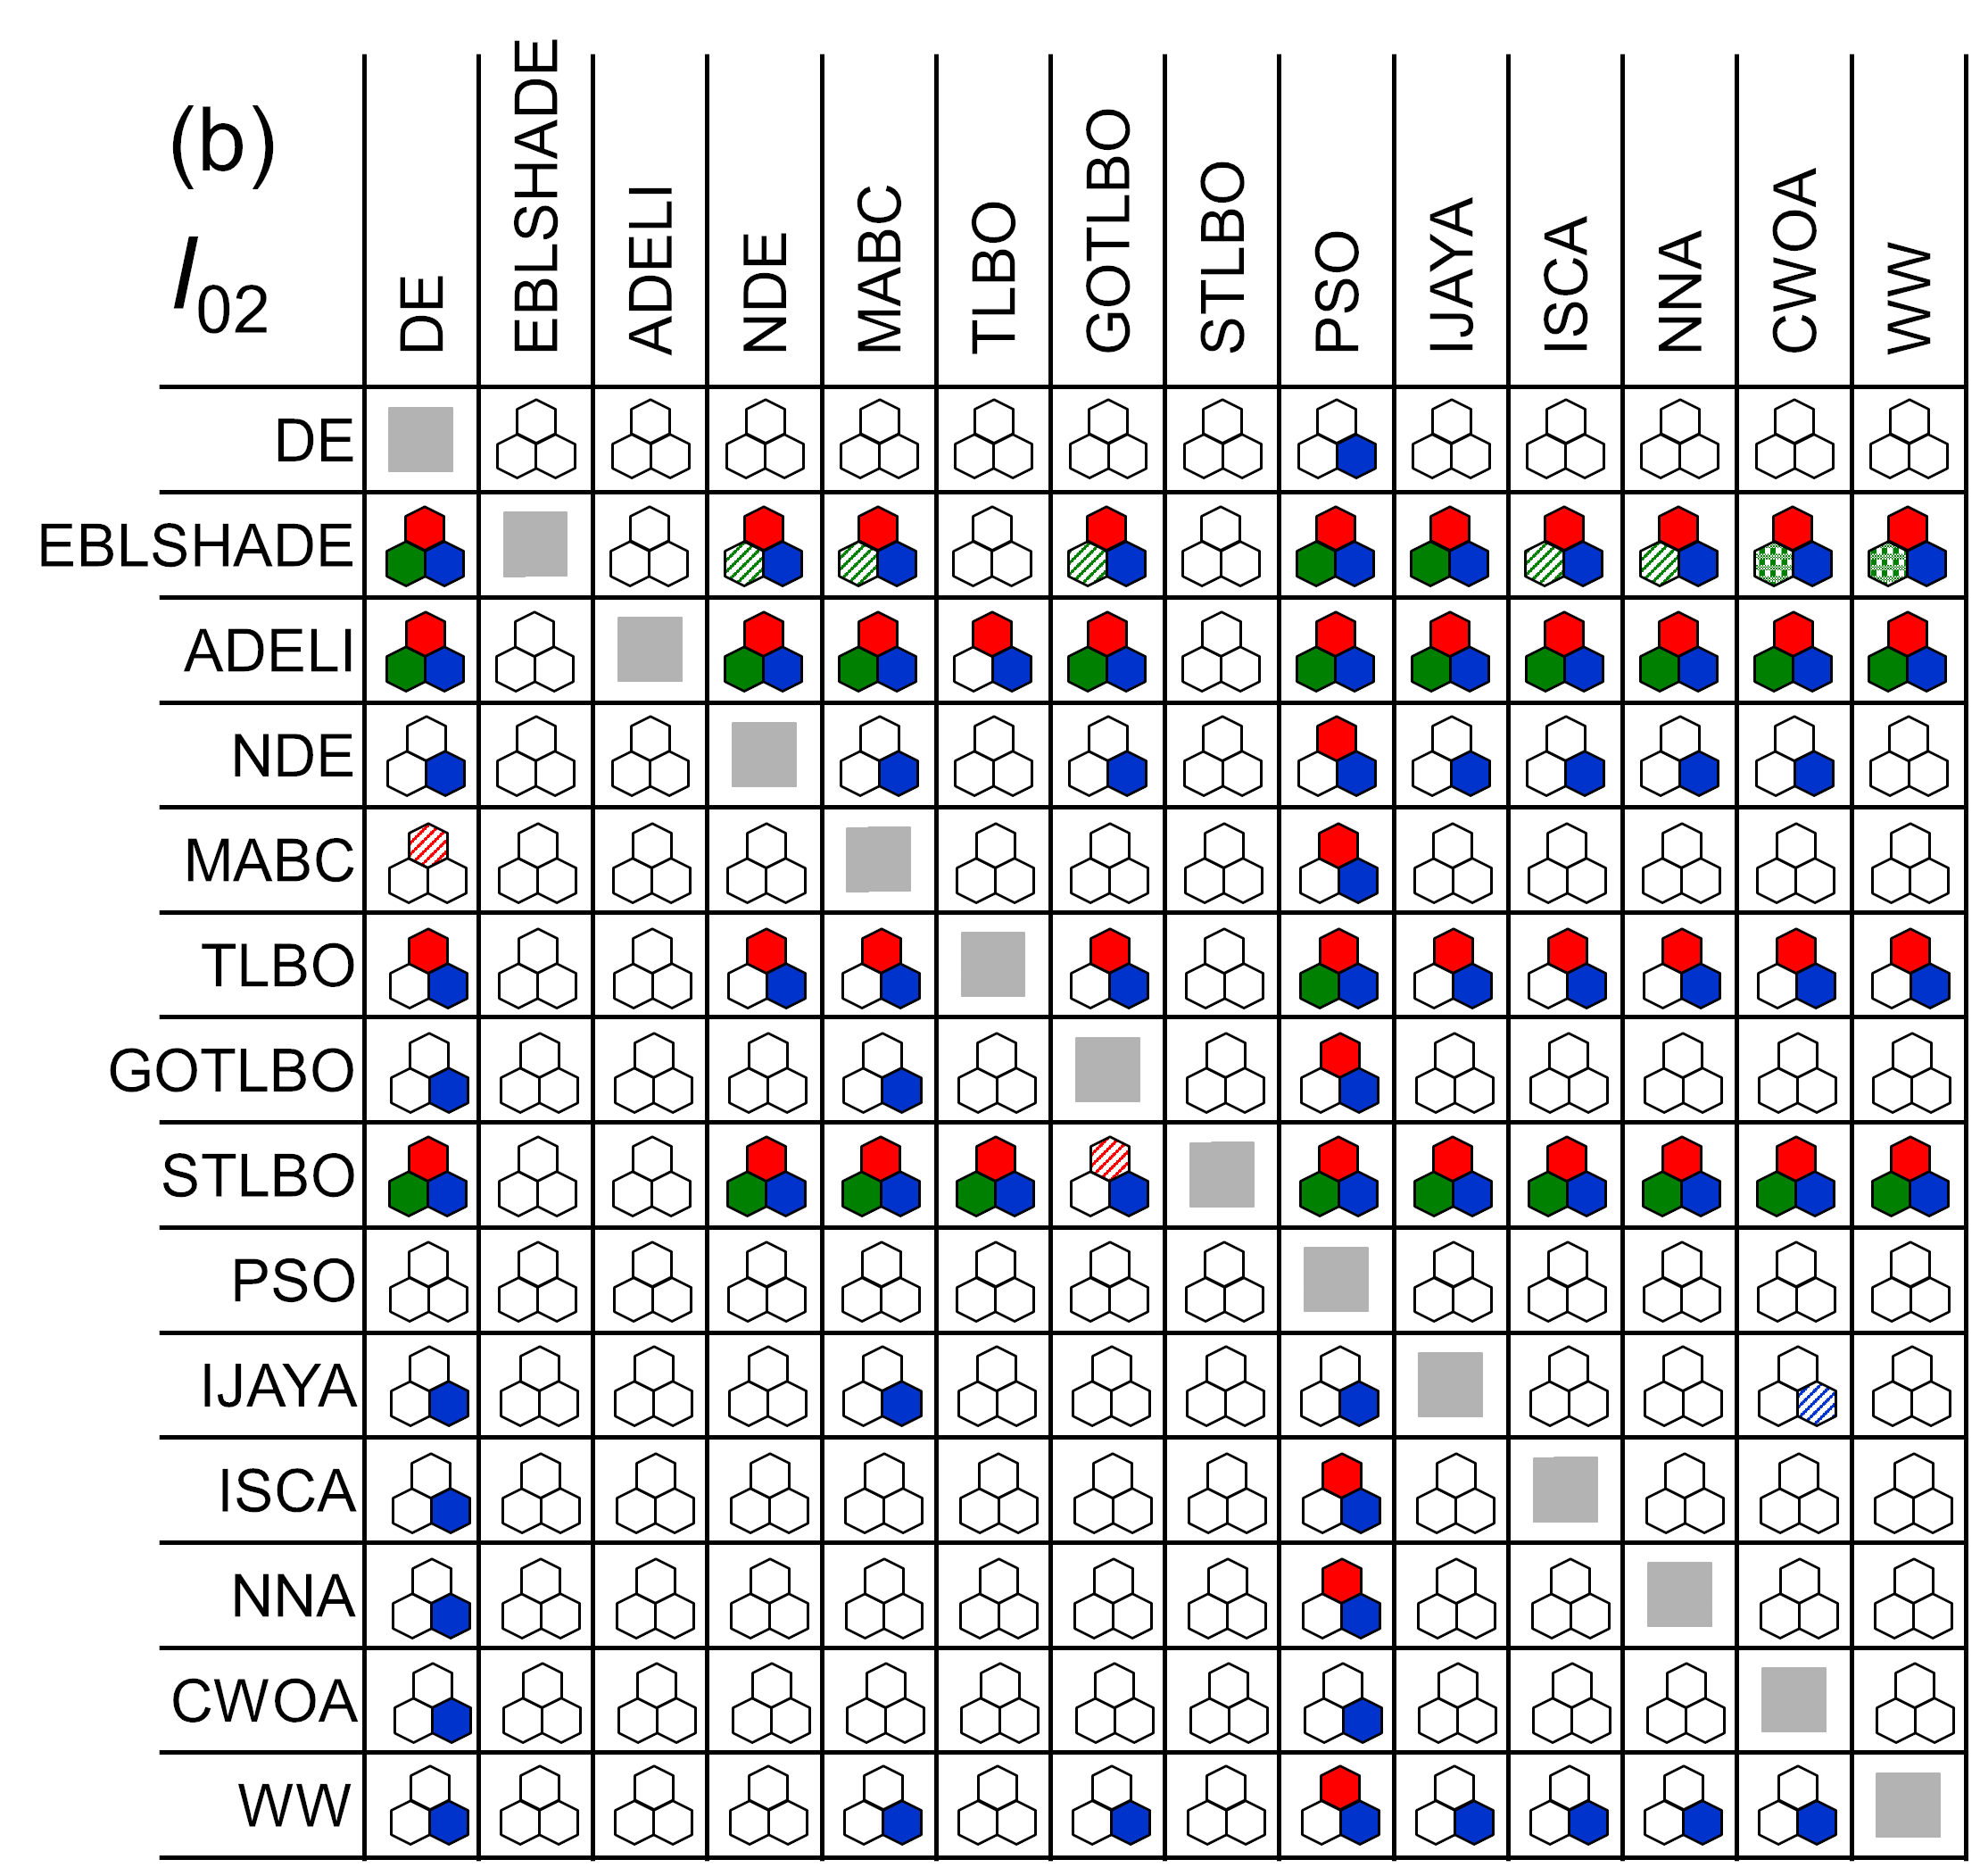
\includegraphics[width=.49\textwidth]{I02shotN1}
        
\includegraphics[width=.48\textwidth]{Titleshot11N}
		
\includegraphics[width=.48\textwidth]{Titleshot21N}
	  \caption{The results of algorithm $1\times N$ comparison in $R_\mathrm{p1}$ (a) and $I_{02}$ (b) evaluation
               by Friedman, Friedman Aligned, and Quade tests in the single--IV case.
               The colored hexagon indicates that the adjusted $p$-value,
               which tests the hypothesis that an algorithm in a row outperforms the algorithm in a column,
               is not greater than $p_{lim}=0.1$.
               The solid fill signifies that every post-hoc procedure resulted in $p<p_{lim}$;
               the patterned fill indicates that only specific post-hoc procedures achieved this outcome.
               The correspondence between the color and position of the hexagon to a test
               as well as the fill pattern to procedures are shown in a legend at the bottom of the figure.
               }\label{figN1RezSingleIV}
\end{figure*}


\begin{table*}[<options>]
\caption{The total number of wins and losses for each algorithm in $1\times N$ multiple comparison using the
Friedman, Friedman Aligned, and Quade tests and Finner, Holm, Hochberg, and Holland post-hoc procedures
in single--IV case.
The criterion for victory was a adjusted $p$-value less than 0.1.
}\label{tbl1NWins}
\begin{tabular*}{\tblwidth}{@{}LCCCCCCCCCCC@{}}
\toprule
\multirow{3}{*}{Algorithm}& \multicolumn{11}{C}{Win / Lose number} \\
&  \multicolumn{10}{C}{task}  &\multirow{2}{*}{Total}\\
  & $I_{01}$& $n_1$ & $R_\mathrm{p1}$ &$I_{02}$& $n_2$& $R_\mathrm{p2}$&$R_\mathrm{s}$&$I_\mathrm{ph}$&RMSPE&Comp&\\ % Table header row
\midrule
DE & 24/43 & 56/34 & 48/35 &  4/73 & 48/43 & 49/34 & 49/40  & 45/35  & 49/48 & 16/27  & 388/412\\
EBLSHADE & 108/\textbf{0} & 108/\textbf{0}  & \textbf{107}/\textbf{0}  & 103/\textbf{0}  & 107/\textbf{0}  & 104/\textbf{0}  & 111/2  & \textbf{105}/\textbf{0}  &  \textbf{109}/\textbf{0}& \textbf{88}/\textbf{0}  & 1050/2 \\
ADELI & \textbf{122}/\textbf{0} & \textbf{110}/\textbf{0}  &  \textbf{107}/\textbf{0} &  \textbf{128}/\textbf{0} &  \textbf{110}/\textbf{0} &  \textbf{122}/\textbf{0} & \textbf{119}/\textbf{0}  & \textbf{105}/\textbf{0}  &  \textbf{109}/\textbf{0}& 61/2  & \textbf{1093}/2\\
NDE & 35/19  & 56/32  & 56/19  & 36/49  & 77/32  & 23/45  &  73/32 & 48/8 & 83/29 & 23/20  & 519/285\\
MABC &  8/61 & 28/69 & 44/45  &  9/57 & 40/55  & 4/82  & 32/51  & 32/66  & 44/62 & 8/30  & 249/578\\
TLBO & 80/3 & 102/\textbf{0} & 101/\textbf{0} &  84/13&  99/\textbf{0}& 87/18 & 93/10 & 94/\textbf{0} & 100/\textbf{0} & 65/2  & 905/46\\
GOTLBO & 8/60  & 12/73  & 4/84  & 16/49  & 20/74  & 13/54 & 20/61  & 4/80 & 16/85  & 13/28  & 126/648\\
STLBO & 109/\textbf{0} & \textbf{110}/\textbf{0}  & \textbf{107}/\textbf{0}  & 125/\textbf{0}  & 107/\textbf{0}  & 119/\textbf{0}  & 116/\textbf{0}  & \textbf{105}/\textbf{0}  & \textbf{109}/\textbf{0} & 81/\textbf{0}  & 1088/\textbf{0}\\
PSO & 0/84  & 8/88  & 0/100  & 0/108  & 4/101  & 0/96  &  0/124 & 0/96  & 20/70  & 4/49  & 72/916\\
IJAYA &  28/28 &  56/34 &  48/35 & 13/52  & 45/43 &  54/34 &  20/61 & 56/29  & 57/38  & 16/34  & 393/388\\
ISCA & 8/56  & 12/76  & 4/84  & 12/45  & 28/65  & 16/51  & 8/61  & 17/68  & 0/92  & 16/32  & 121/630\\
NNA & 33/29  & 0/92  & 4/84  & 12/49  & 12/84  & 12/57  & 8/77  & 12/80  & 0/92& 0/52  & 93/696\\
CWOA & 8/60  & 0/96  &  4/80& 8/52  & 8/84& 4/83  & 20/61  & 0/88  & 0/92 & 0/52  & 52/748\\
WW & 0/96  & 12/76  & 16/76&  36/43 & 0/108 & 10/60 & 12/77  & 12/66  & 0/92& 0/52  & 98/844\\
\bottomrule
\end{tabular*}
\end{table*}


%\begin{table}[<options>]
%\caption{Wilcoxon signed ranks test results of fitness functions comparison with a level of significance $\alpha = 0.05$}\label{tblFF}
%\begin{tabular*}{\tblwidth}{@{}LCCCCCCCCC@{}}
%\toprule
%\multirow{2}{*}{Algorithm}& \multicolumn{9}{C}{Parameter} \\
%  & $I_{01}$& $n_1$ & $R_\mathrm{p1}$ &$I_{02}$& $n_2$& $R_\mathrm{p2}$&$R_\mathrm{s}$&$I_\mathrm{ph}$&RMSPE\\ % Table header row
%\midrule
%DE & SE & SE & = &  = & SE & SE & =  & =  & = \\
%EBLSHADE & SE & =  & =  & =  & =  & =  & =  & =  &  AE \\
%ADELI & SE & =  &  = &  = &  = &  = & =  & =  &   AE\\
%NDE & =  & =  & =  & =  & =  & =  &  = & SE & SE \\
%MABC &  = & SE & =  &  = & =  & =  & =  & =  & SE \\
%TLBO & SE & SE & SE &  SE&  SE& SE & SE & SE & SE \\
%GOTLBO & =  & =  & =  & =  & =  & SE & =  & =  & =  \\
%STLBO & SE & =  & =  & =  & =  & =  & =  & =  &  AE \\
%PSO & =  & =  & =  & =  & =  & =  &  AE & =  & =  \\
%IJAYA &  AE &  AE &  = & =  & SE &  = &  = & =  & =  \\
%ISCA & =  & =  & =  & =  & =  & =  & =  & =  & =  \\
%NNA & =  & =  & =  & =  & =  & =  & =  & =  &  SE\\
%CWOA & =  & =  &  SE& =  &   AE& =  & =  & =  & SE \\
%WW & =  & =  &  SE&  = &  AE &  = & =  & =  &  SE\\
%\bottomrule
%\end{tabular*}
%\end{table}


The statistical results of the algorithm's effectiveness comparison in the task  of $R_\mathrm{p1}$ evaluation are shown in Fig.~\ref{figN1RezSingleIV}(a).
In the figure, the outperforming of an algorithm in a row over the algorithm in the column is indicated by a colored hexagon in the corresponding cell.
The white hexagon suggests a strong likelihood of the null hypothesis.
In fact, the data in Table~\ref{tbl1NADELI} were used to create the third row in Fig.~\ref{figN1RezSingleIV}(a).
The panel (b) of figure presents the statistical results for $I_{02}$ evaluation.
The results of the comparison of algorithms based on the other eight parameters are given in the supplementary materials (figure S2).

\begin{table*}[<options>]
\caption{Adjusted $p$-values for tests for $N\times N$ multiple comparisons of $I_{01}$ evaluation
         among all methods in the single--IV case ($p<1.0$ are only shown).}\label{tblNNpValueI01}
\begin{tabular*}{\tblwidth}{@{}LCCC@{}}
\toprule
\multirow{2}{*}{Hypothesis}& \multicolumn{3}{C}{post-hoc procedure} \\
  &Nemenyi & Holm & Shaffer\\ % Table header row
\midrule
ADELI versus WW&<1E-13&<1E-13&<1E-13\\
ADELI versus NDE&1.17195E-12&1.15907E-12&1.00453E-12\\
STLBO versus CWOA&1.17195E-12&1.15907E-12&1.00453E-12\\
TLBO versus PSO&1.21236E-12&1.17240E-12&1.03917E-12\\
STLBO versus GOTLBO&1.21236E-12&1.17240E-12&1.03917E-12\\
ADELI versus DE&1.73772E-12&1.64224E-12&1.48948E-12\\
STLBO versus DE&1.83875E-12&1.71752E-12&1.57607E-12\\
ADELI versus CWOA&3.83915E-12&3.50164E-12&3.29070E-12\\
EBLSHADE versus GOTLBO&4.20286E-12&3.78719E-12&3.60245E-12\\
STLBO versus NDE&5.01110E-12&4.46043E-12&4.29523E-12\\
ADELI versus GOTLBO&5.41522E-12&4.76064E-12&4.64162E-12\\
EBLSHADE versus CWOA&5.98099E-12&5.19229E-12&5.12657E-12\\
EBLSHADE versus ISCA&1.17195E-11&1.00453E-11&1.00453E-11\\
EBLSHADE versus DE&1.45282E-11&1.22931E-11&1.06966E-11\\
EBLSHADE versus NDE&4.17053E-11&3.43725E-11&3.07061E-11\\
STLBO versus ISCA&8.17133E-11&6.64482E-11&6.01625E-11\\
TLBO versus WW&8.82197E-11&7.07696E-11&6.49529E-11\\
TLBO versus MABC&1.07900E-10&8.53717E-11&7.94431E-11\\
EBLSHADE versus MABC&3.09961E-10&2.38431E-10&2.28213E-10\\
ADELI versus NNA&3.24570E-10&2.46102E-10&2.38969E-10\\
ADELI versus ISCA&3.83410E-10&2.86504E-10&2.82291E-10\\
STLBO versus MABC&1.58351E-09&1.16588E-09&1.16588E-09\\
STLBO versus NNA&1.83408E-09&1.33021E-09&1.33021E-09\\
TLBO versus ISCA&3.49326E-09&2.49519E-09&2.22648E-09\\
ADELI versus MABC&5.83612E-09&4.10452E-09&3.71972E-09\\
EBLSHADE versus NNA&1.23520E-08&8.55140E-09&7.87272E-09\\
EBLSHADE versus PSO&1.47150E-08&1.00256E-08&9.37877E-09\\
STLBO versus PSO&5.32586E-08&3.57008E-08&3.39450E-08\\
ADELI versus PSO&1.50038E-07&9.89261E-08&.56286E-08\\
TLBO versus GOTLBO&2.16253E-07&1.40208E-07&1.37831E-07\\
EBLSHADE versus WW&2.39169E-07&1.52438E-07&1.52438E-07\\
TLBO versus CWOA&2.89034E-07&1.81043E-07&1.77867E-07\\
TLBO versus DE&5.91345E-07&3.63905E-07&3.63905E-07\\
STLBO versus WW&6.86296E-07&4.14794E-07&4.14794E-07\\
TLBO versus NDE&1.37158E-06&8.13904E-07&7.68687E-07\\
TLBO versus NNA&1.17758E-04&6.72904E-05&6.59964E-05\\
NNA versus WW&2.21281E-02&1.24015E-02&1.24015E-02\\
IJAYA versus WW&2.36193E-01&1.29777E-01&1.24585E-01\\
NNA versus PSO&2.36193E-01&1.29777E-01&1.24585E-01\\
NDE versus WW&4.04596E-01&2.13413E-01&2.13413E-01\\
DE versus WW&6.28685E-01&3.24706E-01&3.24706E-01\\
CWOA versus WW&8.94683E-01&4.52257E-01&4.52257E-01\\
GOTLBO versus WW&1.0&5.07626E-01&5.07626E-01\\
IJAYA versus PSO&1.0&8.15876E-01&7.97333E-01\\
NNA versus MABC&1.0&9.64793E-01&9.64793E-01\\
\bottomrule
\end{tabular*}
\end{table*}

The results displayed in Fig.~\ref{figN1RezSingleIV} demonstrate a consistent trend across all parameters. 
Among the compared algorithms, EBLSHADE, ADELI, and STLBO consistently outperform the others in $1\times N$ multiple comparisons. 
On the other hand, algorithms such as PSO, ISCA, CWOA, and NNA consistently produce lower-quality results.
The main changes observed in nonparametric statistical estimation of different parameters evaluation
mainly concern algorithms with moderate effectiveness.

For example, when comparing the accuracy of determining $R_\mathrm{p1}$ and $I_{02}$, 
the IJAYA algorithm performs better in the former case. 
As evident from Figure 3a, 
IJAYA outperforms GOTLBO, PSO, ISCA, NNA, CWOA, and WW in the results of Friedman 
and Friedman Aligned tests for every post-hoc procedure considered.
While for $I_{02}$, IJAYA only outperforms DE, MABC, PSO, and CWOA according to the Friedman test, 
and in the latter case, only for Finner post-hoc procedure.
For DE, the situation is similar in the case of $I_{02}$ compared to $R_\mathrm{p1}$. 
According to the results of the Friedman and Friedman Aligned tests, the algorithm loses its advantage over GOTLBO, SCA, NNA, CWOA, and WW.
Additionally, the Friedman test no longer shows the improvement of DE over PSO.



\begin{figure*}[!ht]
	\centering
		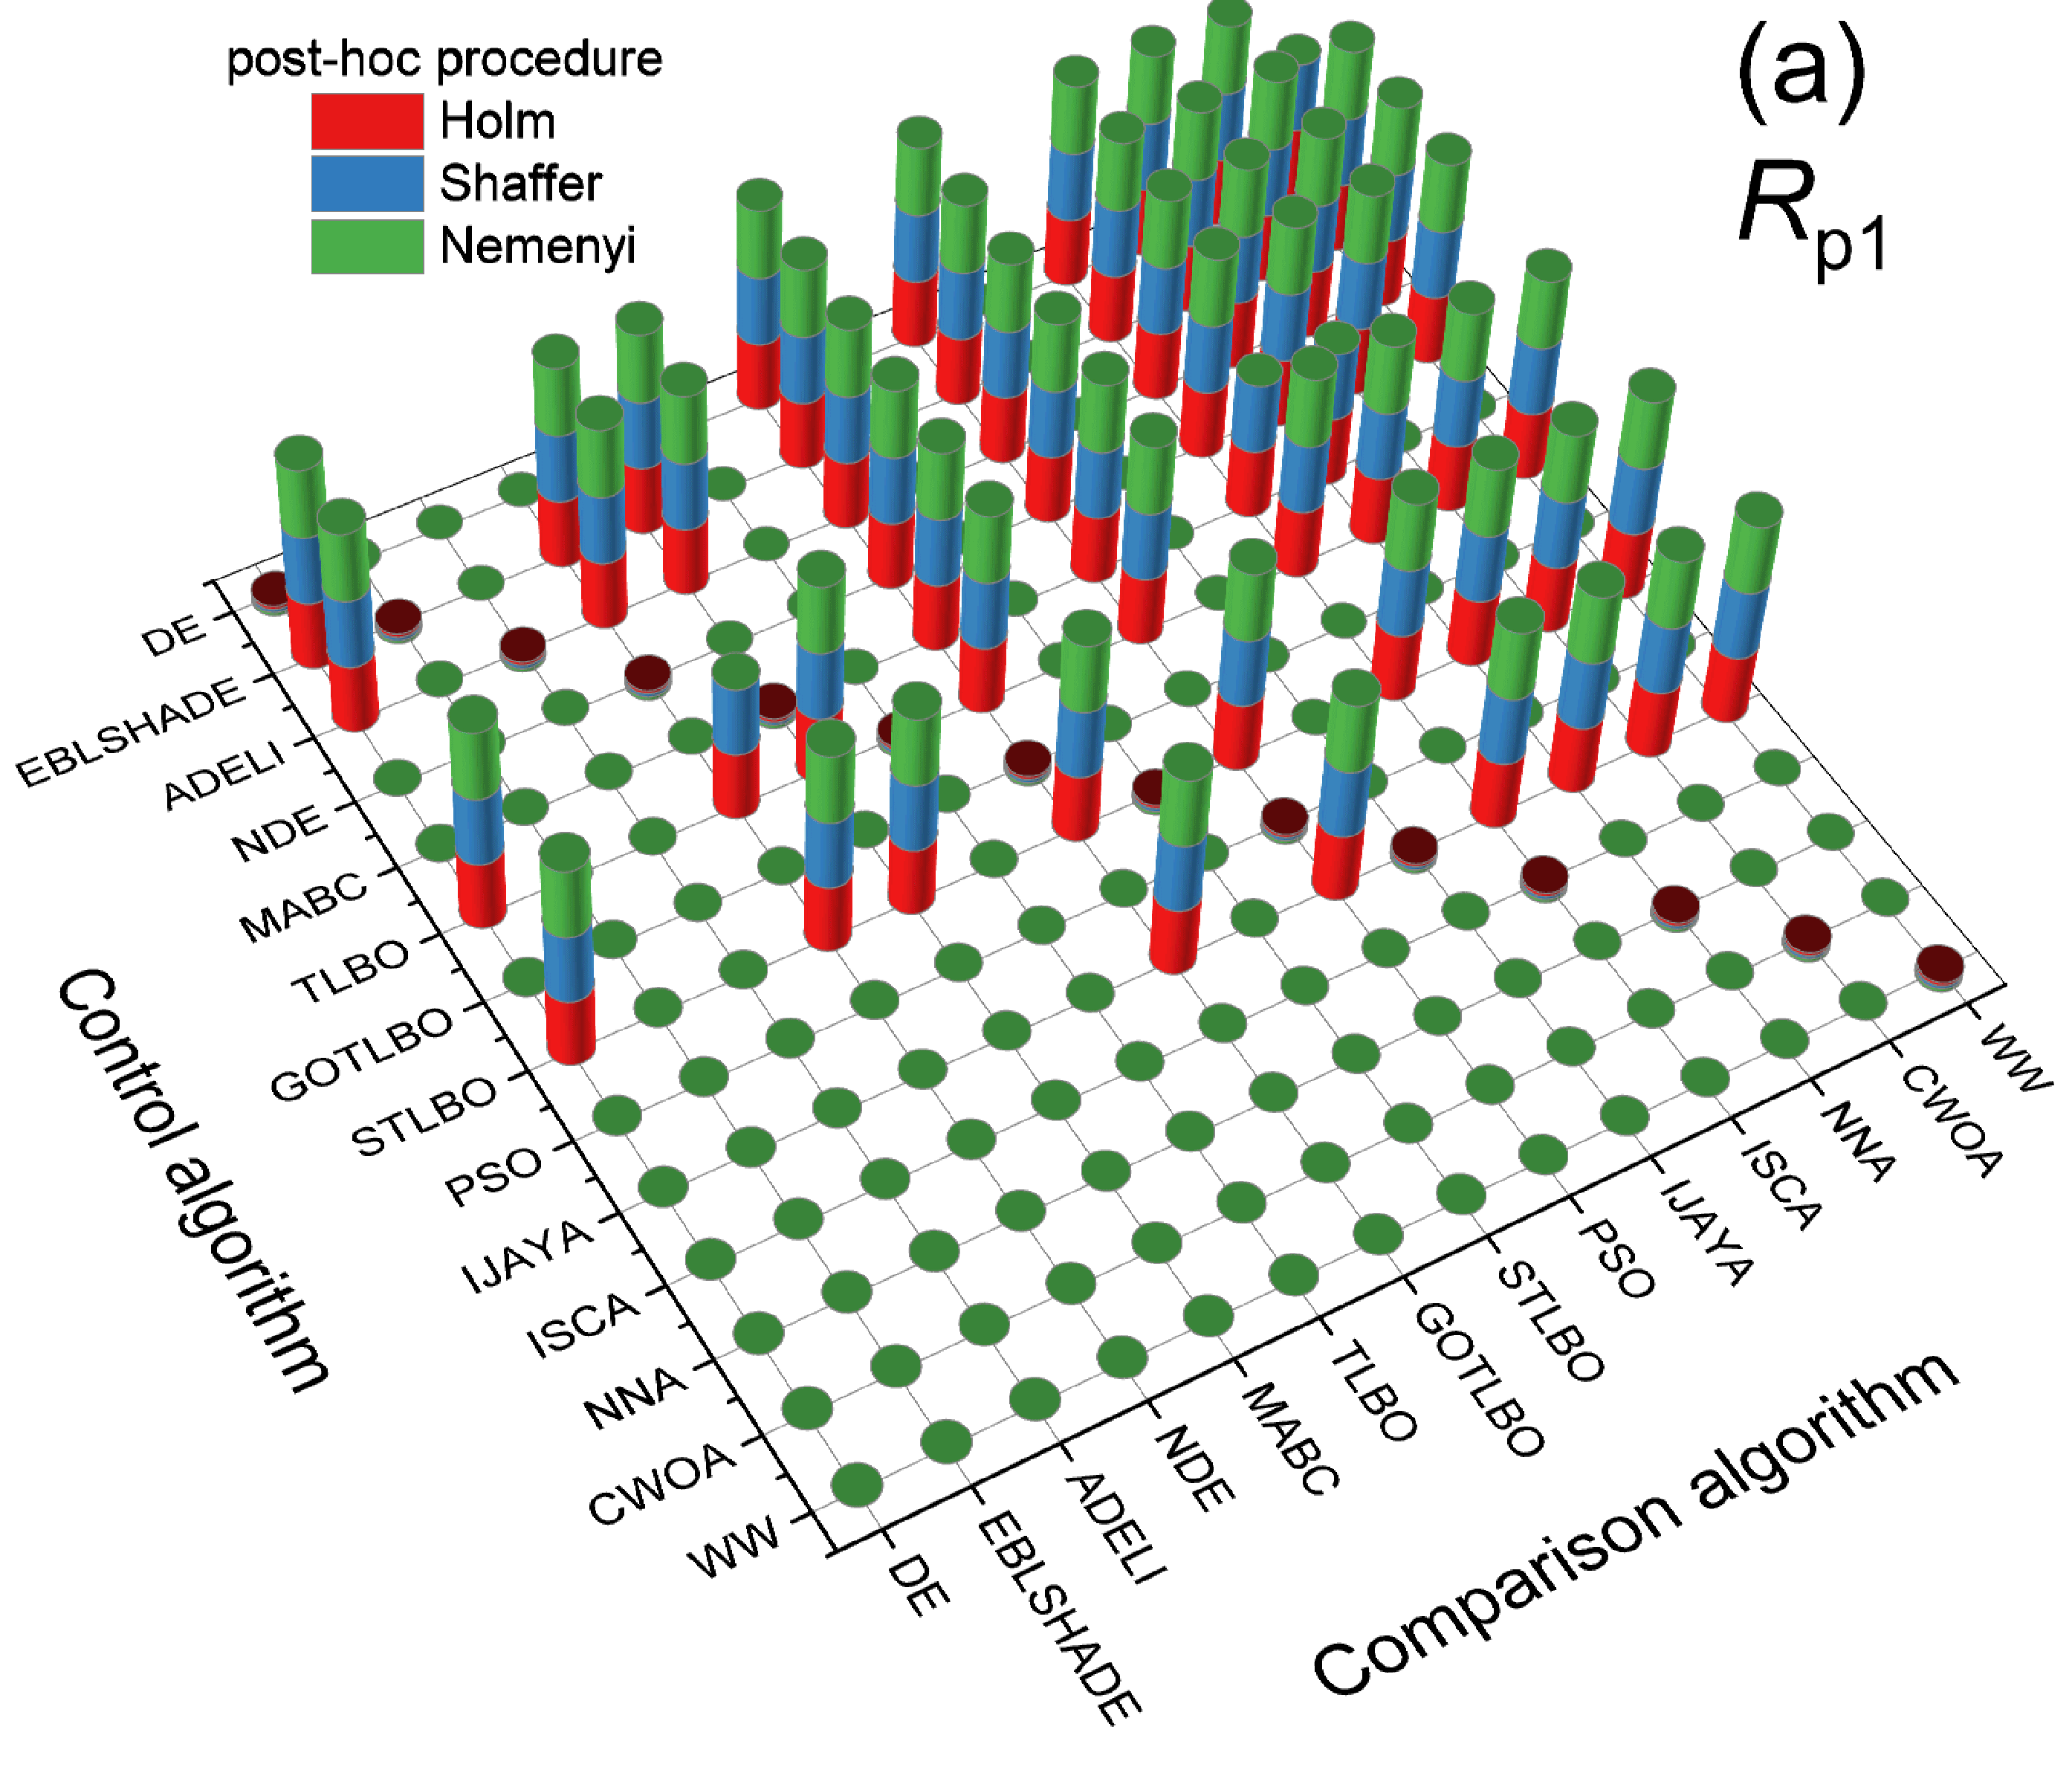
\includegraphics[width=.49\textwidth]{Rp1shot_NN}
        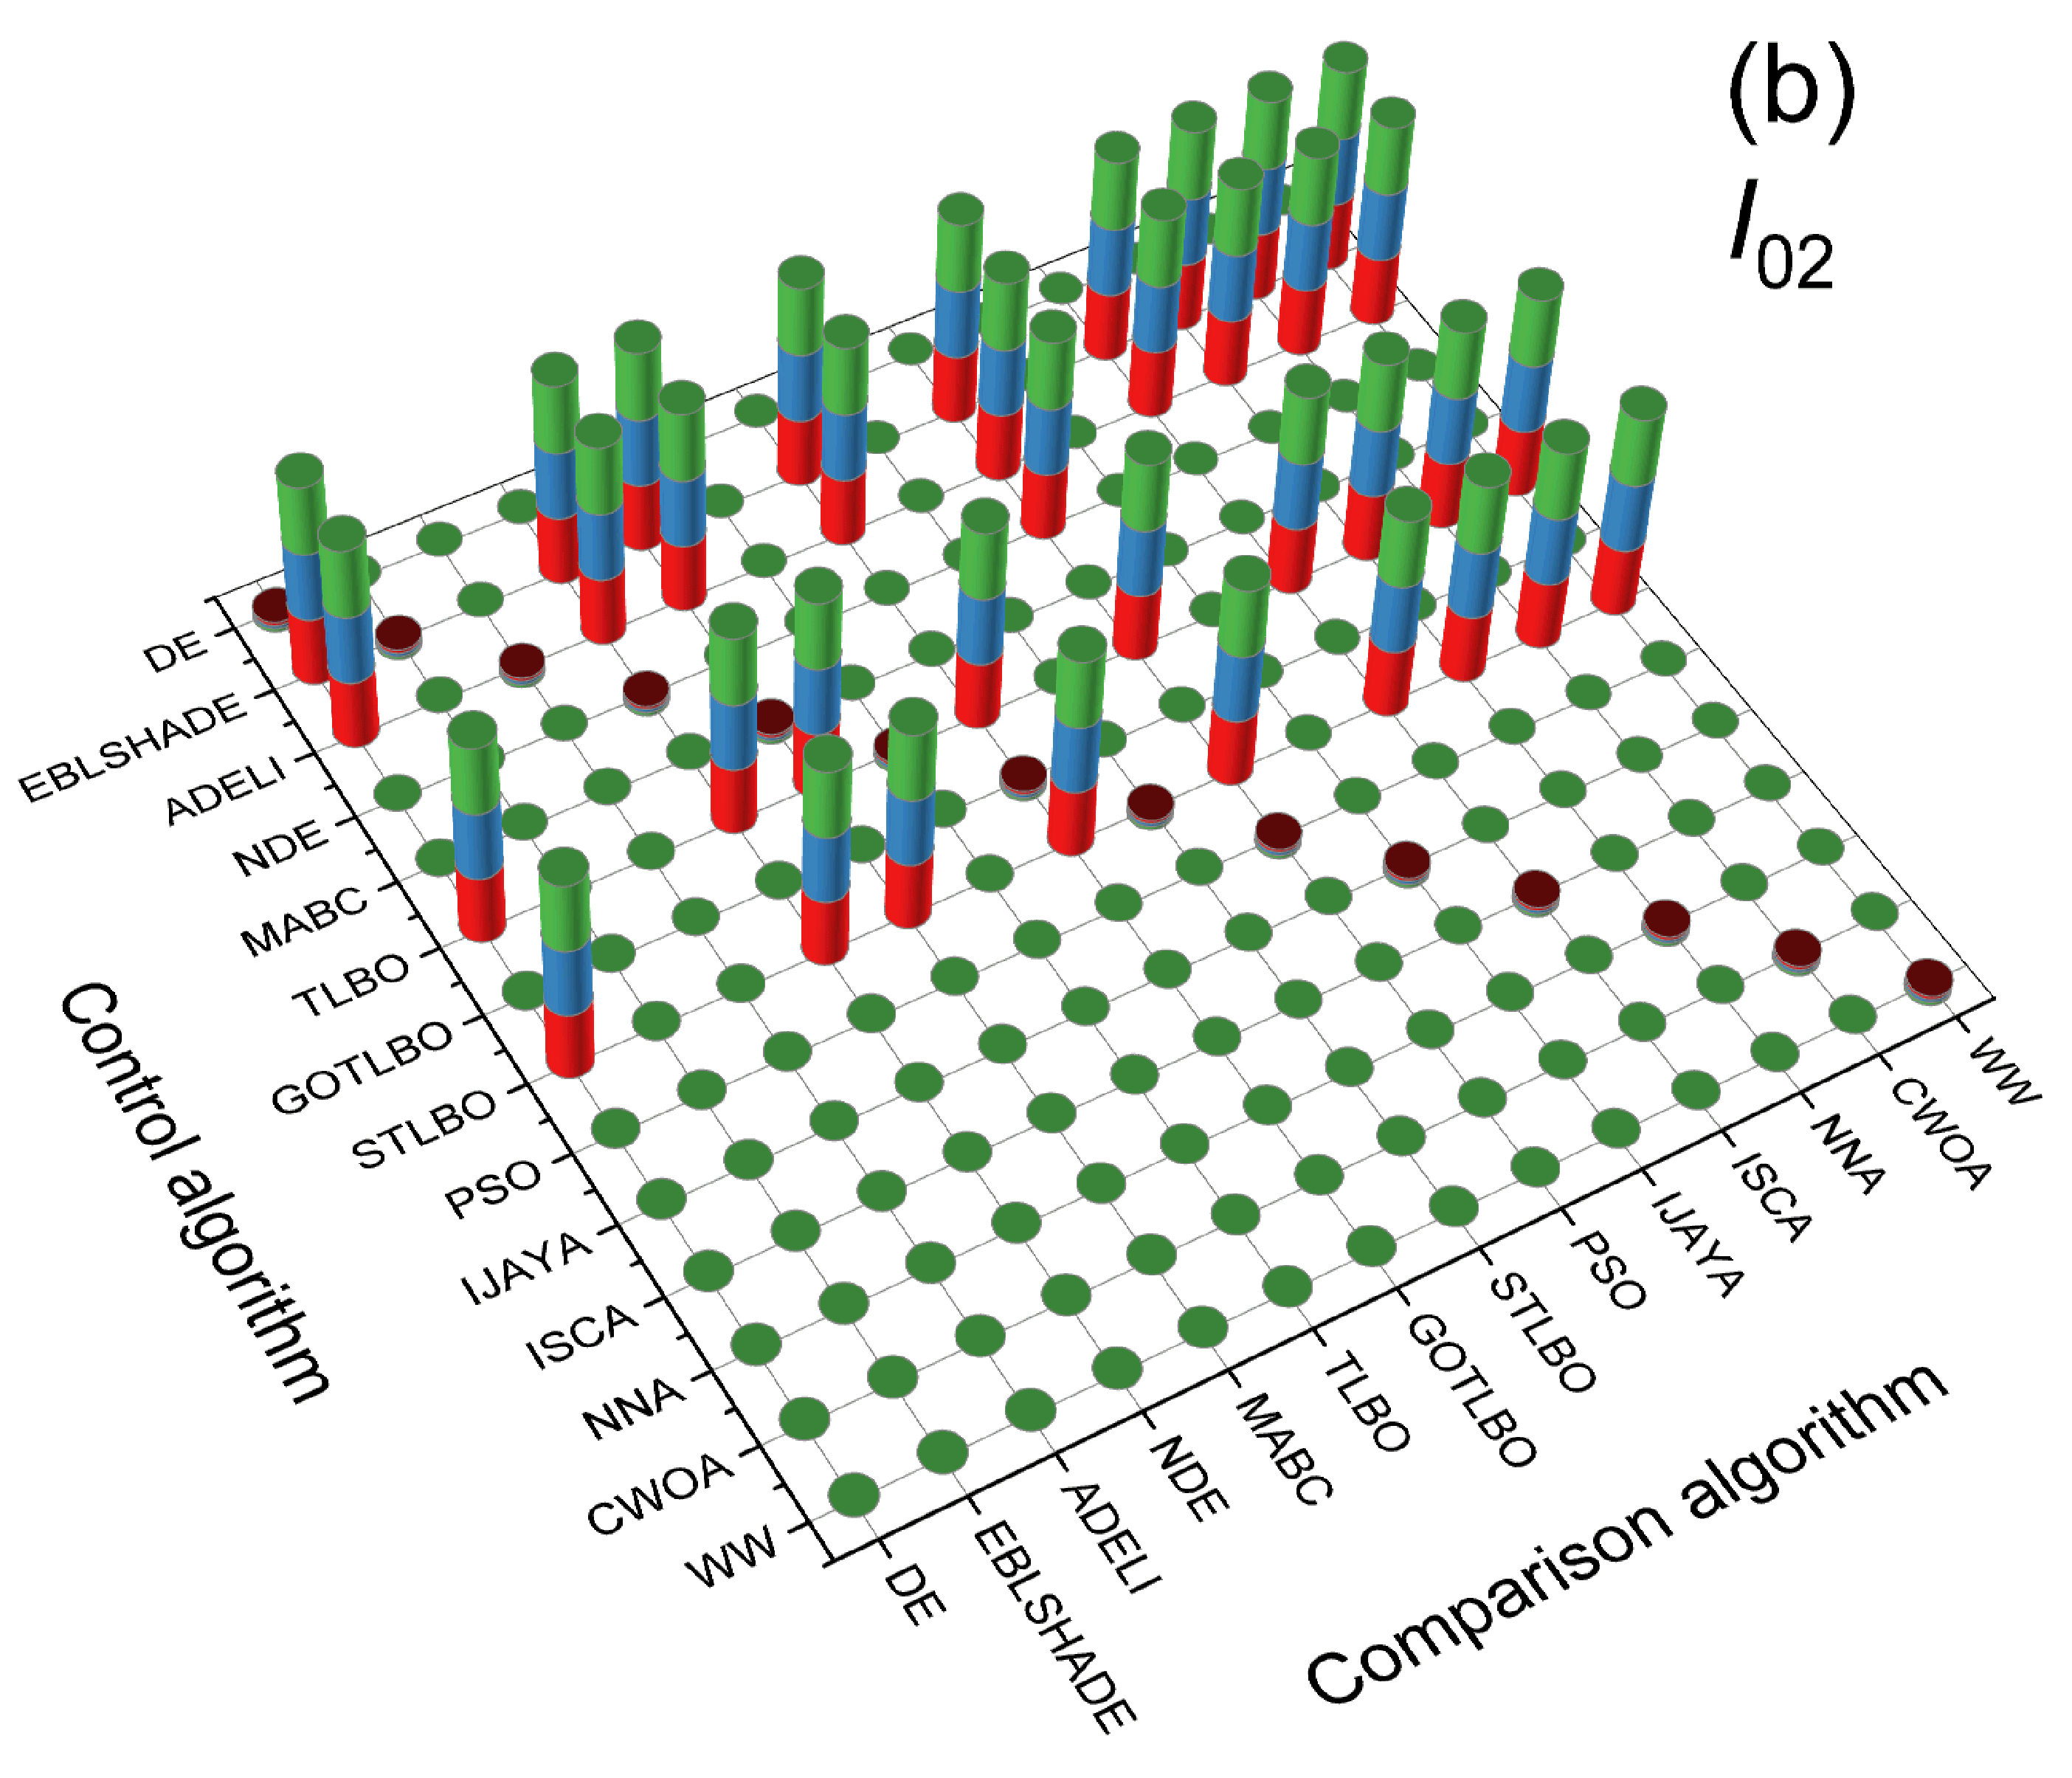
\includegraphics[width=.49\textwidth]{I02shot_NN}
	  \caption{The results of $N\times N$ multiple comparisons of $R_\mathrm{p1}$ (a) and $I_{02}$ (b) evaluation
               among all algorithms in the single--IV case.
               The colored cylinder indicates that the adjusted $p$-value,
               which tests the control algorithm outperforms the comparison algorithm,
               is not greater than $p_{lim}=0.1$.
               The correspondence between the color of the cylinder to a post-hoc procedure is shown in the figure's legend.
               }\label{figNNRezSingleIV}
\end{figure*}

\begin{table*}[<options>]
\caption{The total number of wins and losses for each algorithm in $N\times N$ multiple comparison using the
Friedman test and Shaffer's static, Nemenyi, and Holm post-hoc procedures
in single--IV case.
The criterion for victory was a adjusted $p$-value less than 0.1.
}\label{tblNNWins}
\begin{tabular*}{\tblwidth}{@{}LCCCCCCCCCCC@{}}
\toprule
\multirow{3}{*}{Algorithm}& \multicolumn{11}{C}{Win / Lose number} \\
&  \multicolumn{10}{C}{task}  &\multirow{2}{*}{Total}\\
  & $I_{01}$& $n_1$ & $R_\mathrm{p1}$ &$I_{02}$& $n_2$& $R_\mathrm{p2}$&$R_\mathrm{s}$&$I_\mathrm{ph}$&RMSPE&Comp&\\ % Table header row
\midrule
DE & 0/12 & 17/12 & 17/12 &  0/12 & 12/12 & 14/12 & 5/12  & 17/12  & 15/15 & 0/0  & 97/111\\
EBLSHADE & 27/0 & 27/0  & 27/0  & 27/0  & 27/0  & 27/0  & 27/0 & 27/0  &  26/0& 21/0  & \textbf{263}/\textbf{0} \\
ADELI & 27/0 & 27/0  &  27/0 &  27/0 &  27/0 &  27/0 & 27/0  & 27/0  &  27/0& 14/0  & 257/\textbf{0}\\
NDE & 0/12  & 21/12  & 18/11  & 3/12  & 18/9  & 3/12  &  18/11 & 21/9 & 24/8 & 0/0  & 126/96\\
MABC &  0/12& 0/15& 10/12  &  0/12 & 11/12  & 0/17  & 3/12  & 2/15  & 12/15 & 0/3  & 38/125\\
TLBO & 27/0& 27/0 & 26/0 &  27/0&  24/0& 27/0 & 26/0 & 24/0 & 24/0 & 10/0  & 242/0\\
GOTLBO & 0/12  & 0/18  & 0/24  & 0/12  & 3/15  & 0/12 & 3/15  & 0/21 & 0/21  & 0/5  & 6/155\\
STLBO & 27/0 & 27/0  & 27/0  & 27/0  & 27/0  & 27/0  & 27/0  & 27/0  & 27/0 & 11/0  & 254/\textbf{0}\\
PSO & 0/12  & 0/21  & 0/24  & 0/15  & 0/24  & 0/21  &  0/34 & 0/23  & 0/18  & 0/12  & 0/204\\
IJAYA &  0/0 &  16/0 &  18/0 & 0/0  & 12/0 &  11/0 &  3/0 & 18/0  & 18/0  & 0/0  & 96/\textbf{0}\\
ISCA & 0/12  & 0/21  & 0/23  & 0/12  & 3/15  & 0/12  & 2/15  & 0/21  & 0/24 & 0/3  & 5/158\\
NNA & 3/12  & 0/21  & 0/23  & 0/12  & 0/23  & 0/14  & 0/17  & 0/21  & 0/24& 0/9  & 3/176\\
CWOA & 0/12  & 0/21  &  0/21& 0/12  & 0/24& 0/18  & 3/15  & 0/21  & 0/24 & 0/12  & 3/180\\
WW & 0/15  & 0/21  & 0/20&  0/12 & 0/30 & 0/18 & 2/15  & 0/20  & 0/24& 0/12  & 2/187\\
\bottomrule
\end{tabular*}
\end{table*}

In all cases, the Quade test yields higher adjusted $p$-values.
In particular, in the case of the complex parameter, none of the conducted comparisons exceeded the chosen threshold value of the $p$-value.

The adjusted $p$-values obtained from the direct comparison of EBLSHADE, ADELI, and STLBO
do not allow for determining the best algorithm among them.
However, for this purpose, the results of this top trio of algorithms can be used,
obtained from their comparison with less efficient optimization methods.
Table~\ref{tbl1NWins} summarizes number of wins and losses for each algorithm in $1\times N$ multiple comparison.
The maximum possible number of wins achieved in every 10 tasks is 156,
obtained from comparing with 13 algorithms in 3 tests using 4 procedures.
As can be seen, among the compared algorithms,
ADELI showed the highest number of statistically confirmed improvements (1093) over others,
indicating its superior performance.
Conversely, STLBO demonstrated the lowest number of defeats (0) in similar comparisons, suggesting its consistently strong performance.

Previously, we employed procedures that controlled the Family-Wise Error Rate (FWER)
for comparisons with a control algorithm.
We tested each of the 14 algorithms individually to determine if any of them were superior to the others.
Below are the results of the carried out a multiple comparison in which
all possible pairwise comparisons need to be computed ( $N\times N$ comparison),
and three procedures (Shaffer’s static, Nemenyi, and Holm) have been used to control FWER.
These procedures take into account that the hypotheses being tested belonging
to a family of all pairwise comparisons are logically interrelated;
thus not all combinations of true and false hypotheses are possible.

Starting from the analysis performed by the Friedman test over our results, we can raise the
91 hypotheses of equality among the 14 algorithms of our study for each task,
and apply the methods mentioned earlier to contrast them.
Table~\ref{tblNNpValueI01} lists the part of the hypotheses
and the adjusted $p$-values achieved on the task of $I_{01}$ evaluation.
For the remaining 46 hypotheses not indicated in the table,
a $p$-value of 1 was obtained after applying each of the procedures.
The full version of the table as well as the data, obtained for other task,
are given in the supplementary material (tables~S144-S153).

It can be seen that using a level of significance 0.1, only 37 hypotheses
are rejected by the Nemenyi, Holm, and Shaffer methods.
These hypotheses show the improvement of EBLSHADE, ADELI,  TLBO, and STLBO
over DE, NDE, MABC, GOTLBO, PSO, ISCA, NNA, CWOA, and WW,
and NNA over WW.
None of the remaining 54 hypotheses can be rejected using these procedures.

%  & $I_{01}$& $n_1$ & $R_\mathrm{p1}$ &$I_{02}$& $n_2$& $R_\mathrm{p2}$&$R_\mathrm{s}$&$I_\mathrm{ph}$&RMSPE\\ % Table header row
%DE, EBLSHADE, ADELI, NDE, MABC, TLBO, GOTLBO, STLBO, PSO, IJAYA, ISCA, NNA, CWOA, WW


%$\mathrm{APE}_\mathrm{MEAN}$
%перекласти на англійську "Результати порівняння алгоритмів за іншими восьмами параметрів подані в додаткових матеріалах"


%The energy band diagram of the inverted device structure ITO/ZnO/PTB7:PC71BM/MoO3/Ag is given in
%the supplementary material (figure S1 is available online at stacks.iop.org/MRX/5/116203/mmedia).
% The cell parameters obtained from the J-V characteristics are tabulated
%(table S1 in the supplementary material).
%Light intensity dependent C-F plots for the
%devices with 70, 150 and 250 nm ZnO layer thicknesses are given in the supplementary material (figure S2)
%The presence of leakage current can be
%correlated with the shunt resistance (Rsh) values obtained from the dark J-V curve (table S1 in thesupplementary
%material).
%The reader is referred to supplementary material for more information on the simulated BHJ morphologies.28
%The reader is referred to the supplementary material for more information on the cut-off
%approximation.
%However, in the supplementary material28 we show that for the aforementioned
%trap densities the trap population is essentially a small perturbation to the total energy landscape and the reduction in the
%standard deviation of energetic disorder is negligible.
%This saturation effect was also seen in the
%evolution of exciton diffusion with trap depth (see supplementary material28).



%62]. Tables 5 and 6 give the statistical results produced by
%Wilcoxon sign-rank test with a significant level α = 0.05.
%In Tables 5 and 6, R+ means the sum of ranks for the
%problems in which EJAYA outperformed the compared algorithm and R− indicates the sum of ranks for the opposite.
%As can be seen from Tables 5 and 6, there are the following
%three cases:
%(1) Case 1: If R+ is more than R− and the obtained
%p-value is less than the set significant level α, the
%symbol is marked with ‘+’ and EJAYA outperforms
%the compared algorithm on the considered case.


\subsubsection{Evaluation of IV--set}

\begin{figure*}[]
	\centering
		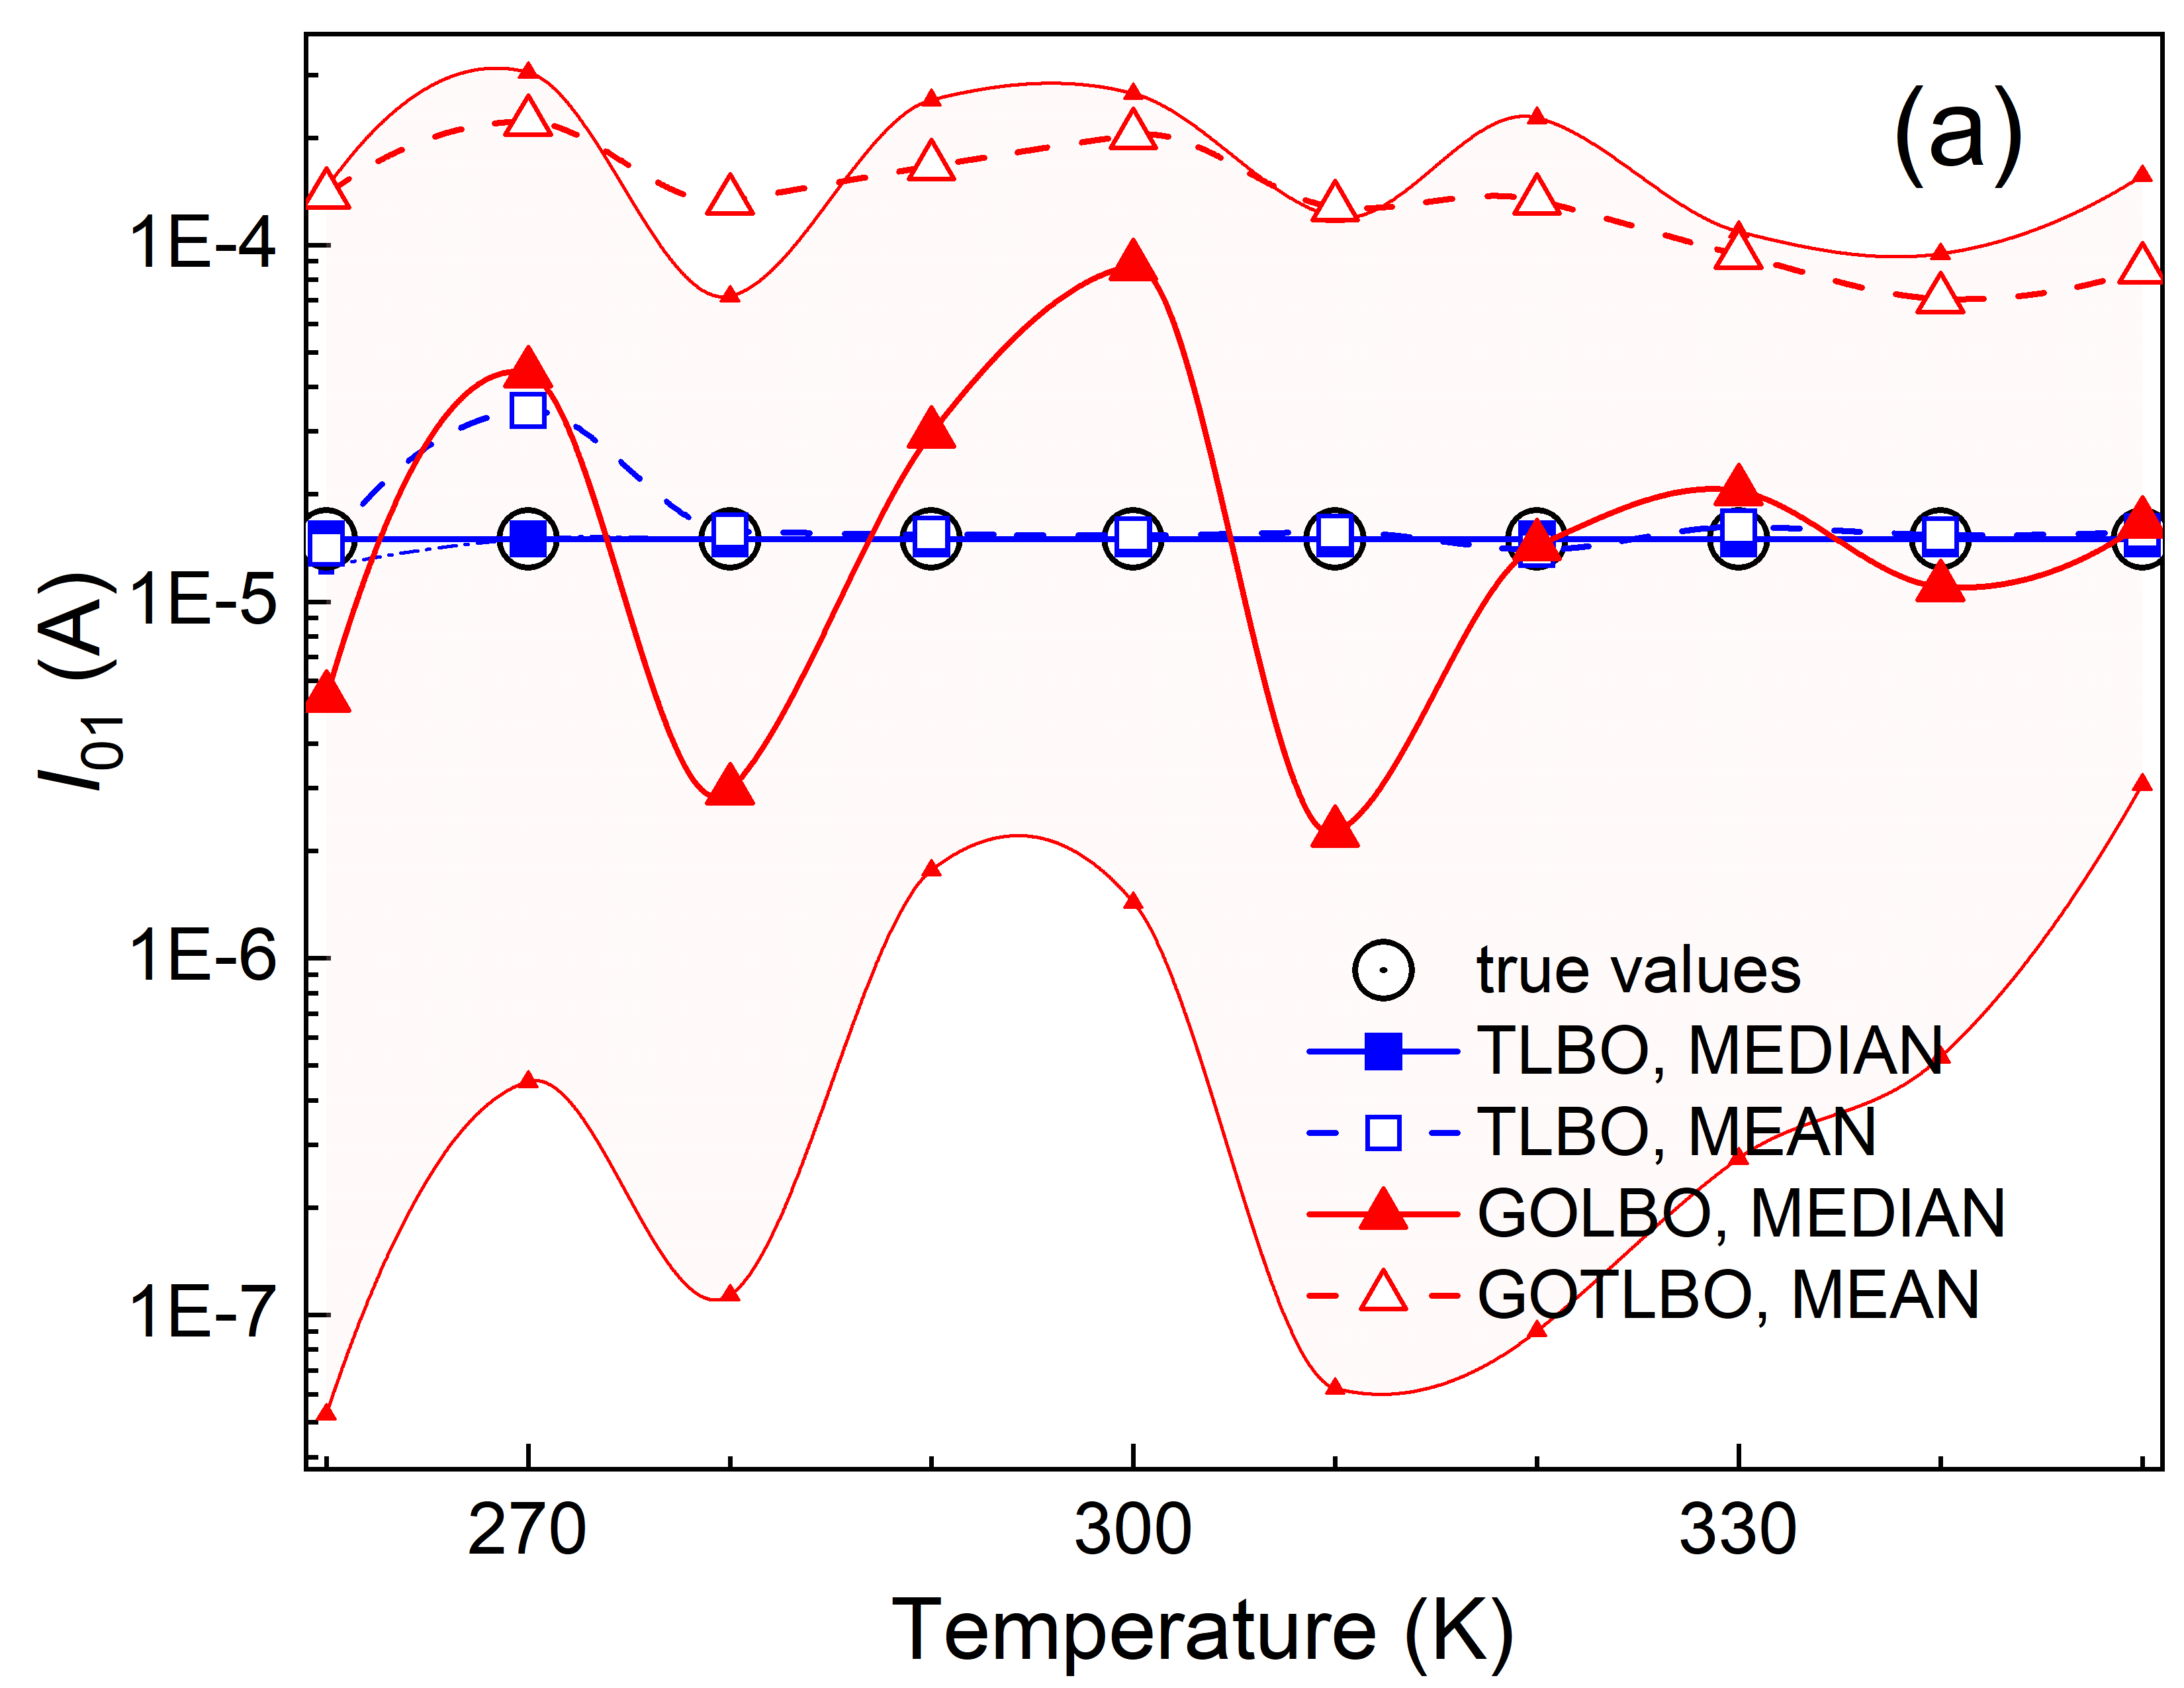
\includegraphics[width=.32\textwidth]{AfigA}
        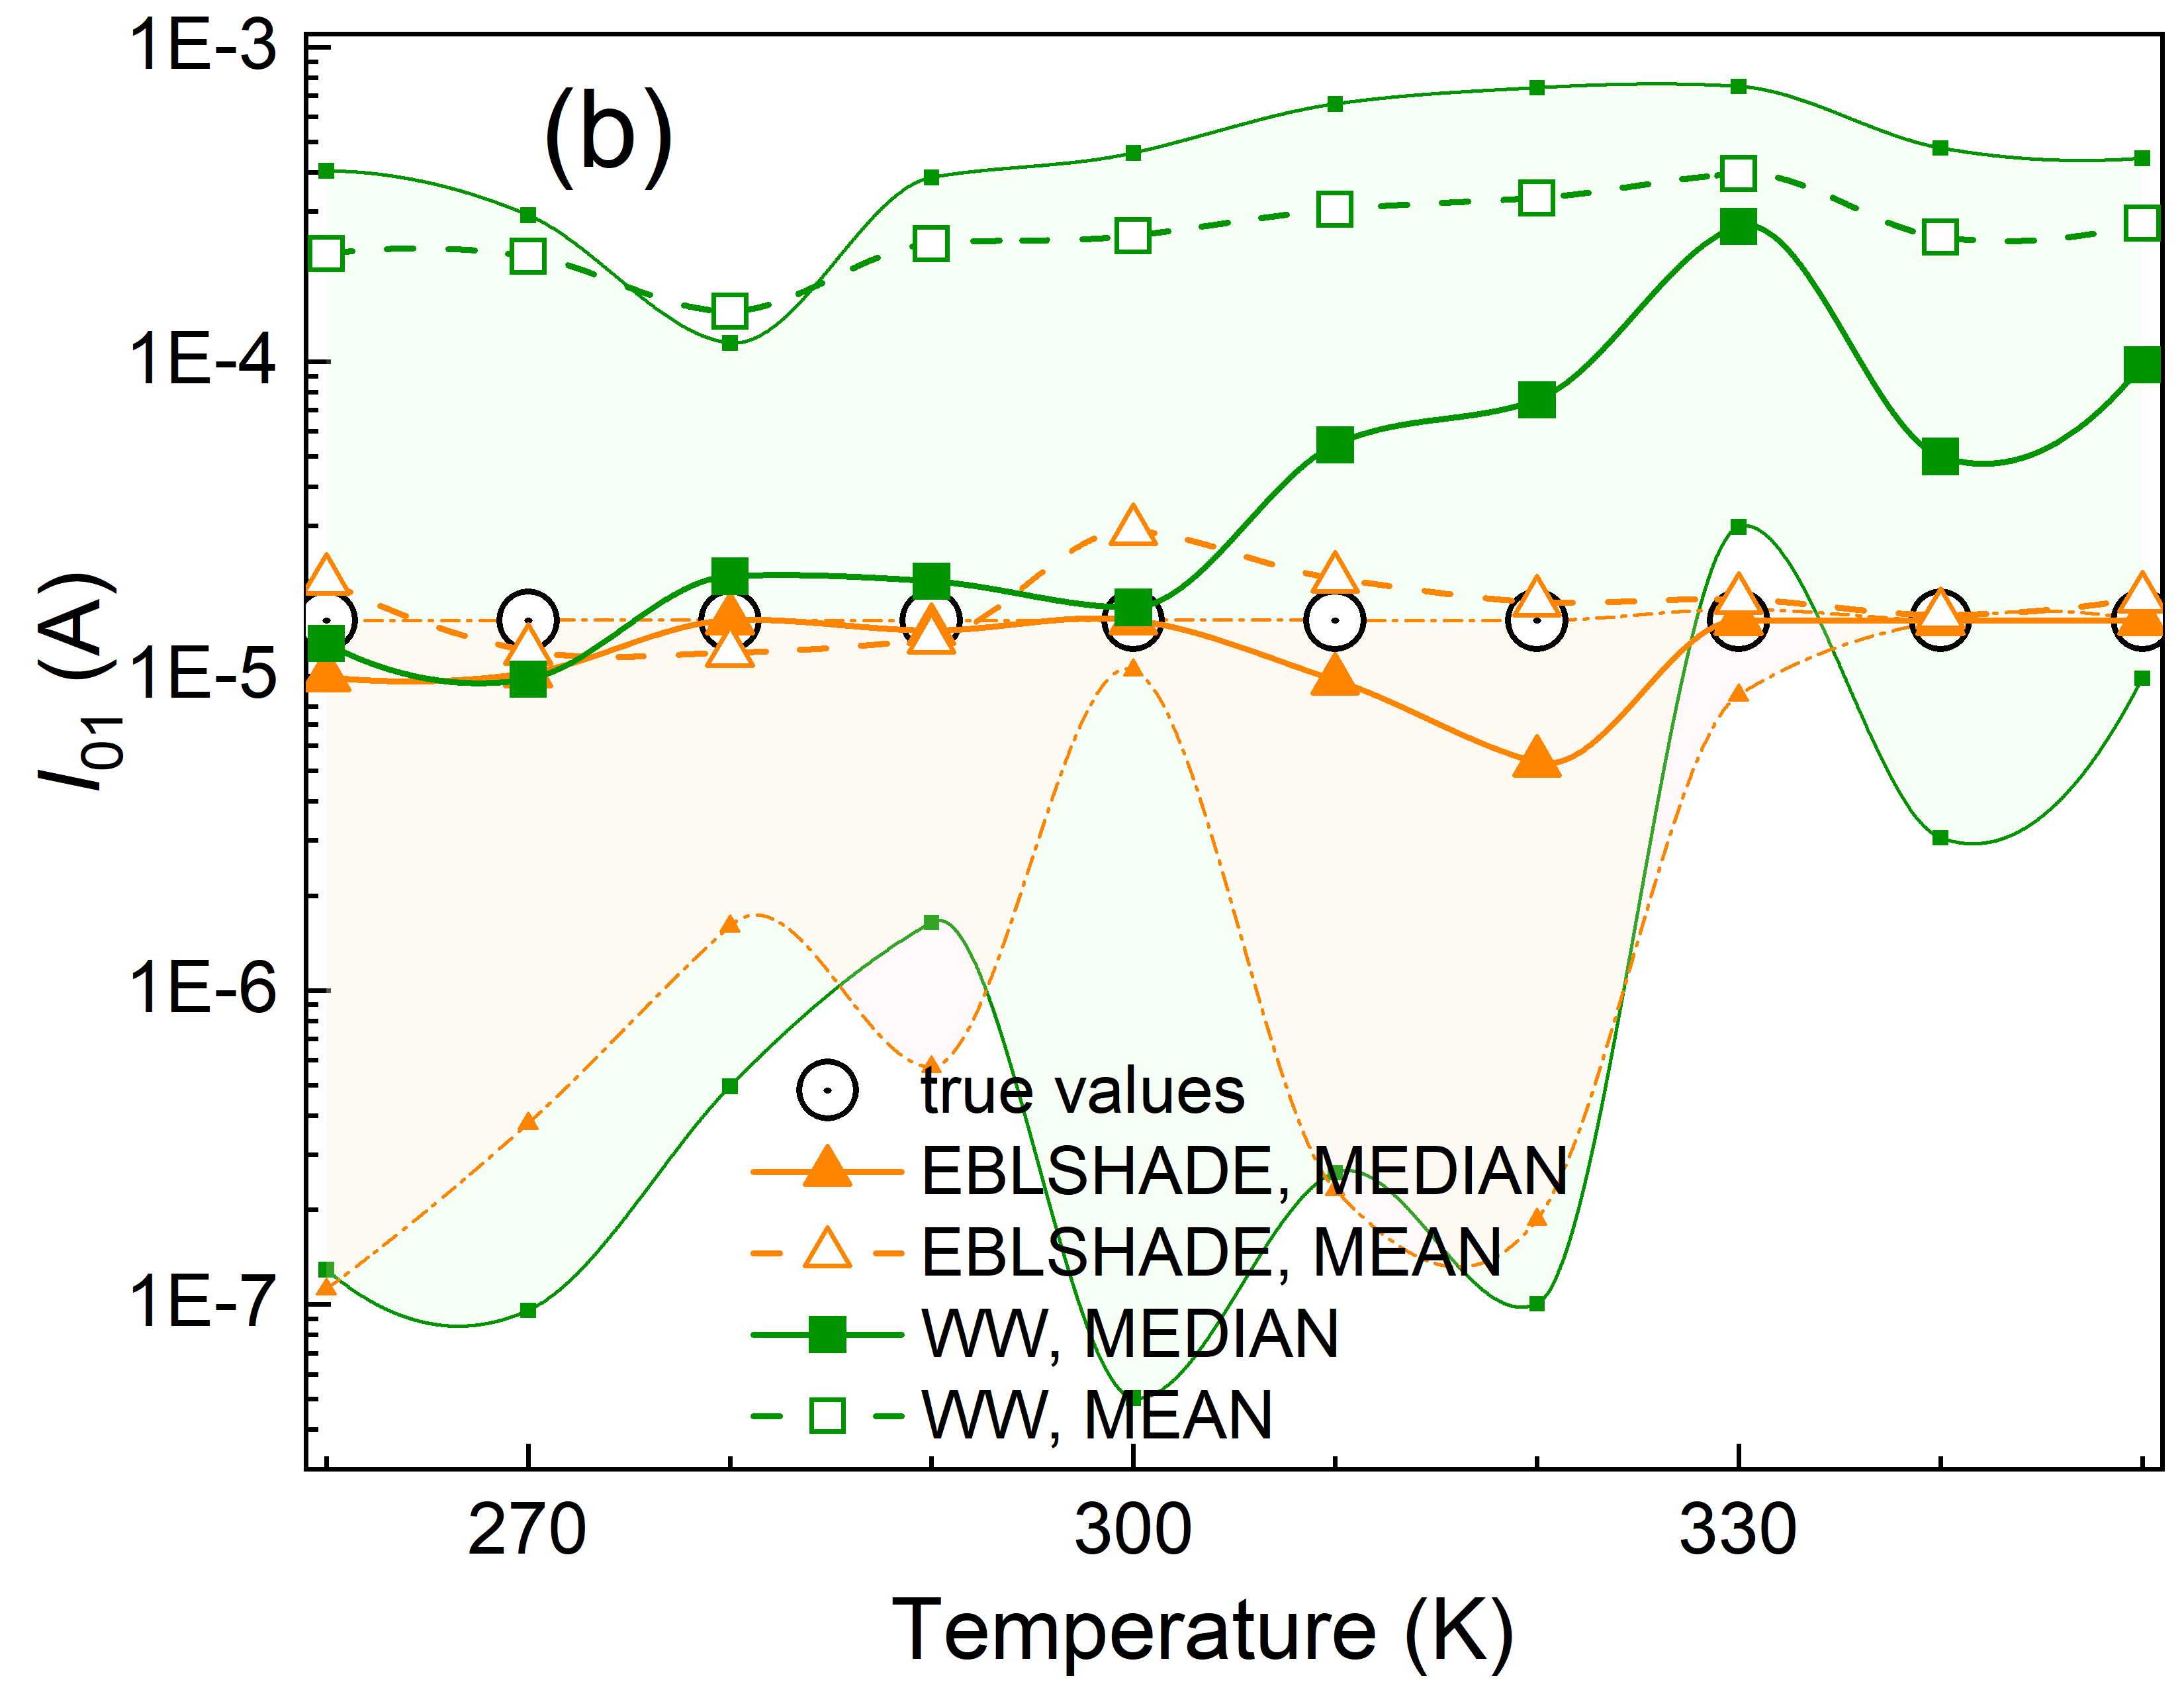
\includegraphics[width=.32\textwidth]{AfigB}
        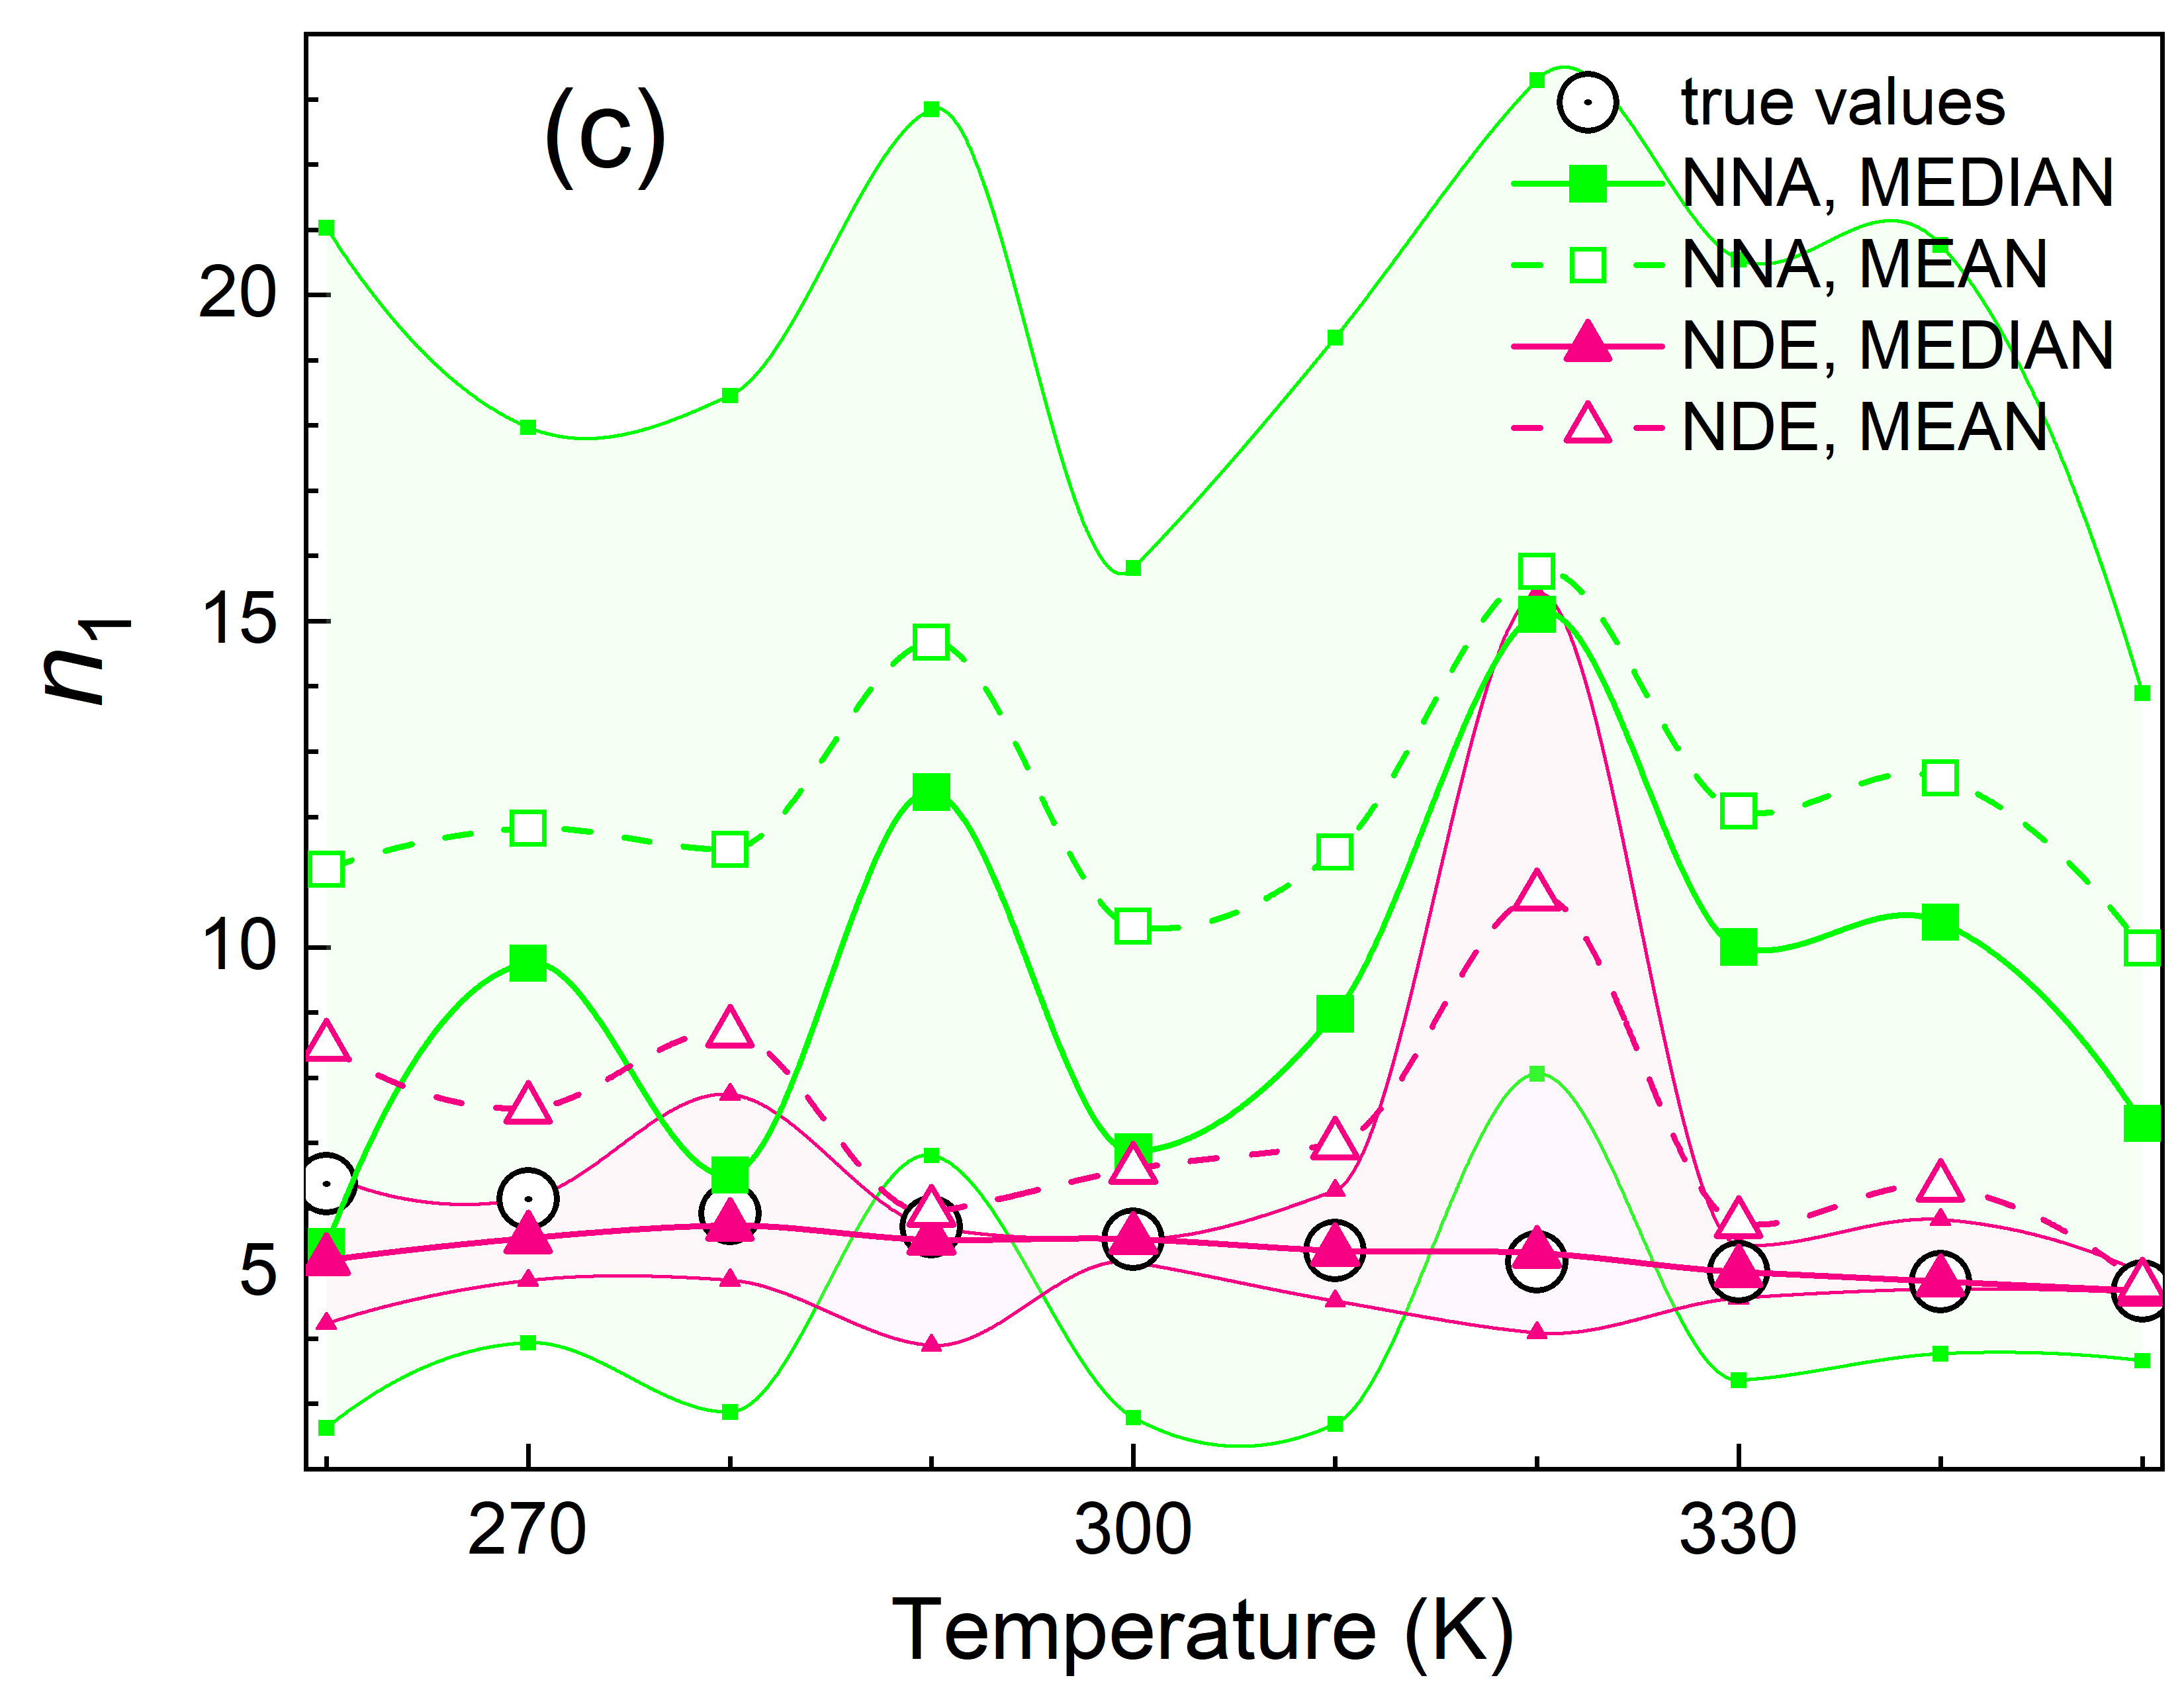
\includegraphics[width=.32\textwidth]{AfigC}
		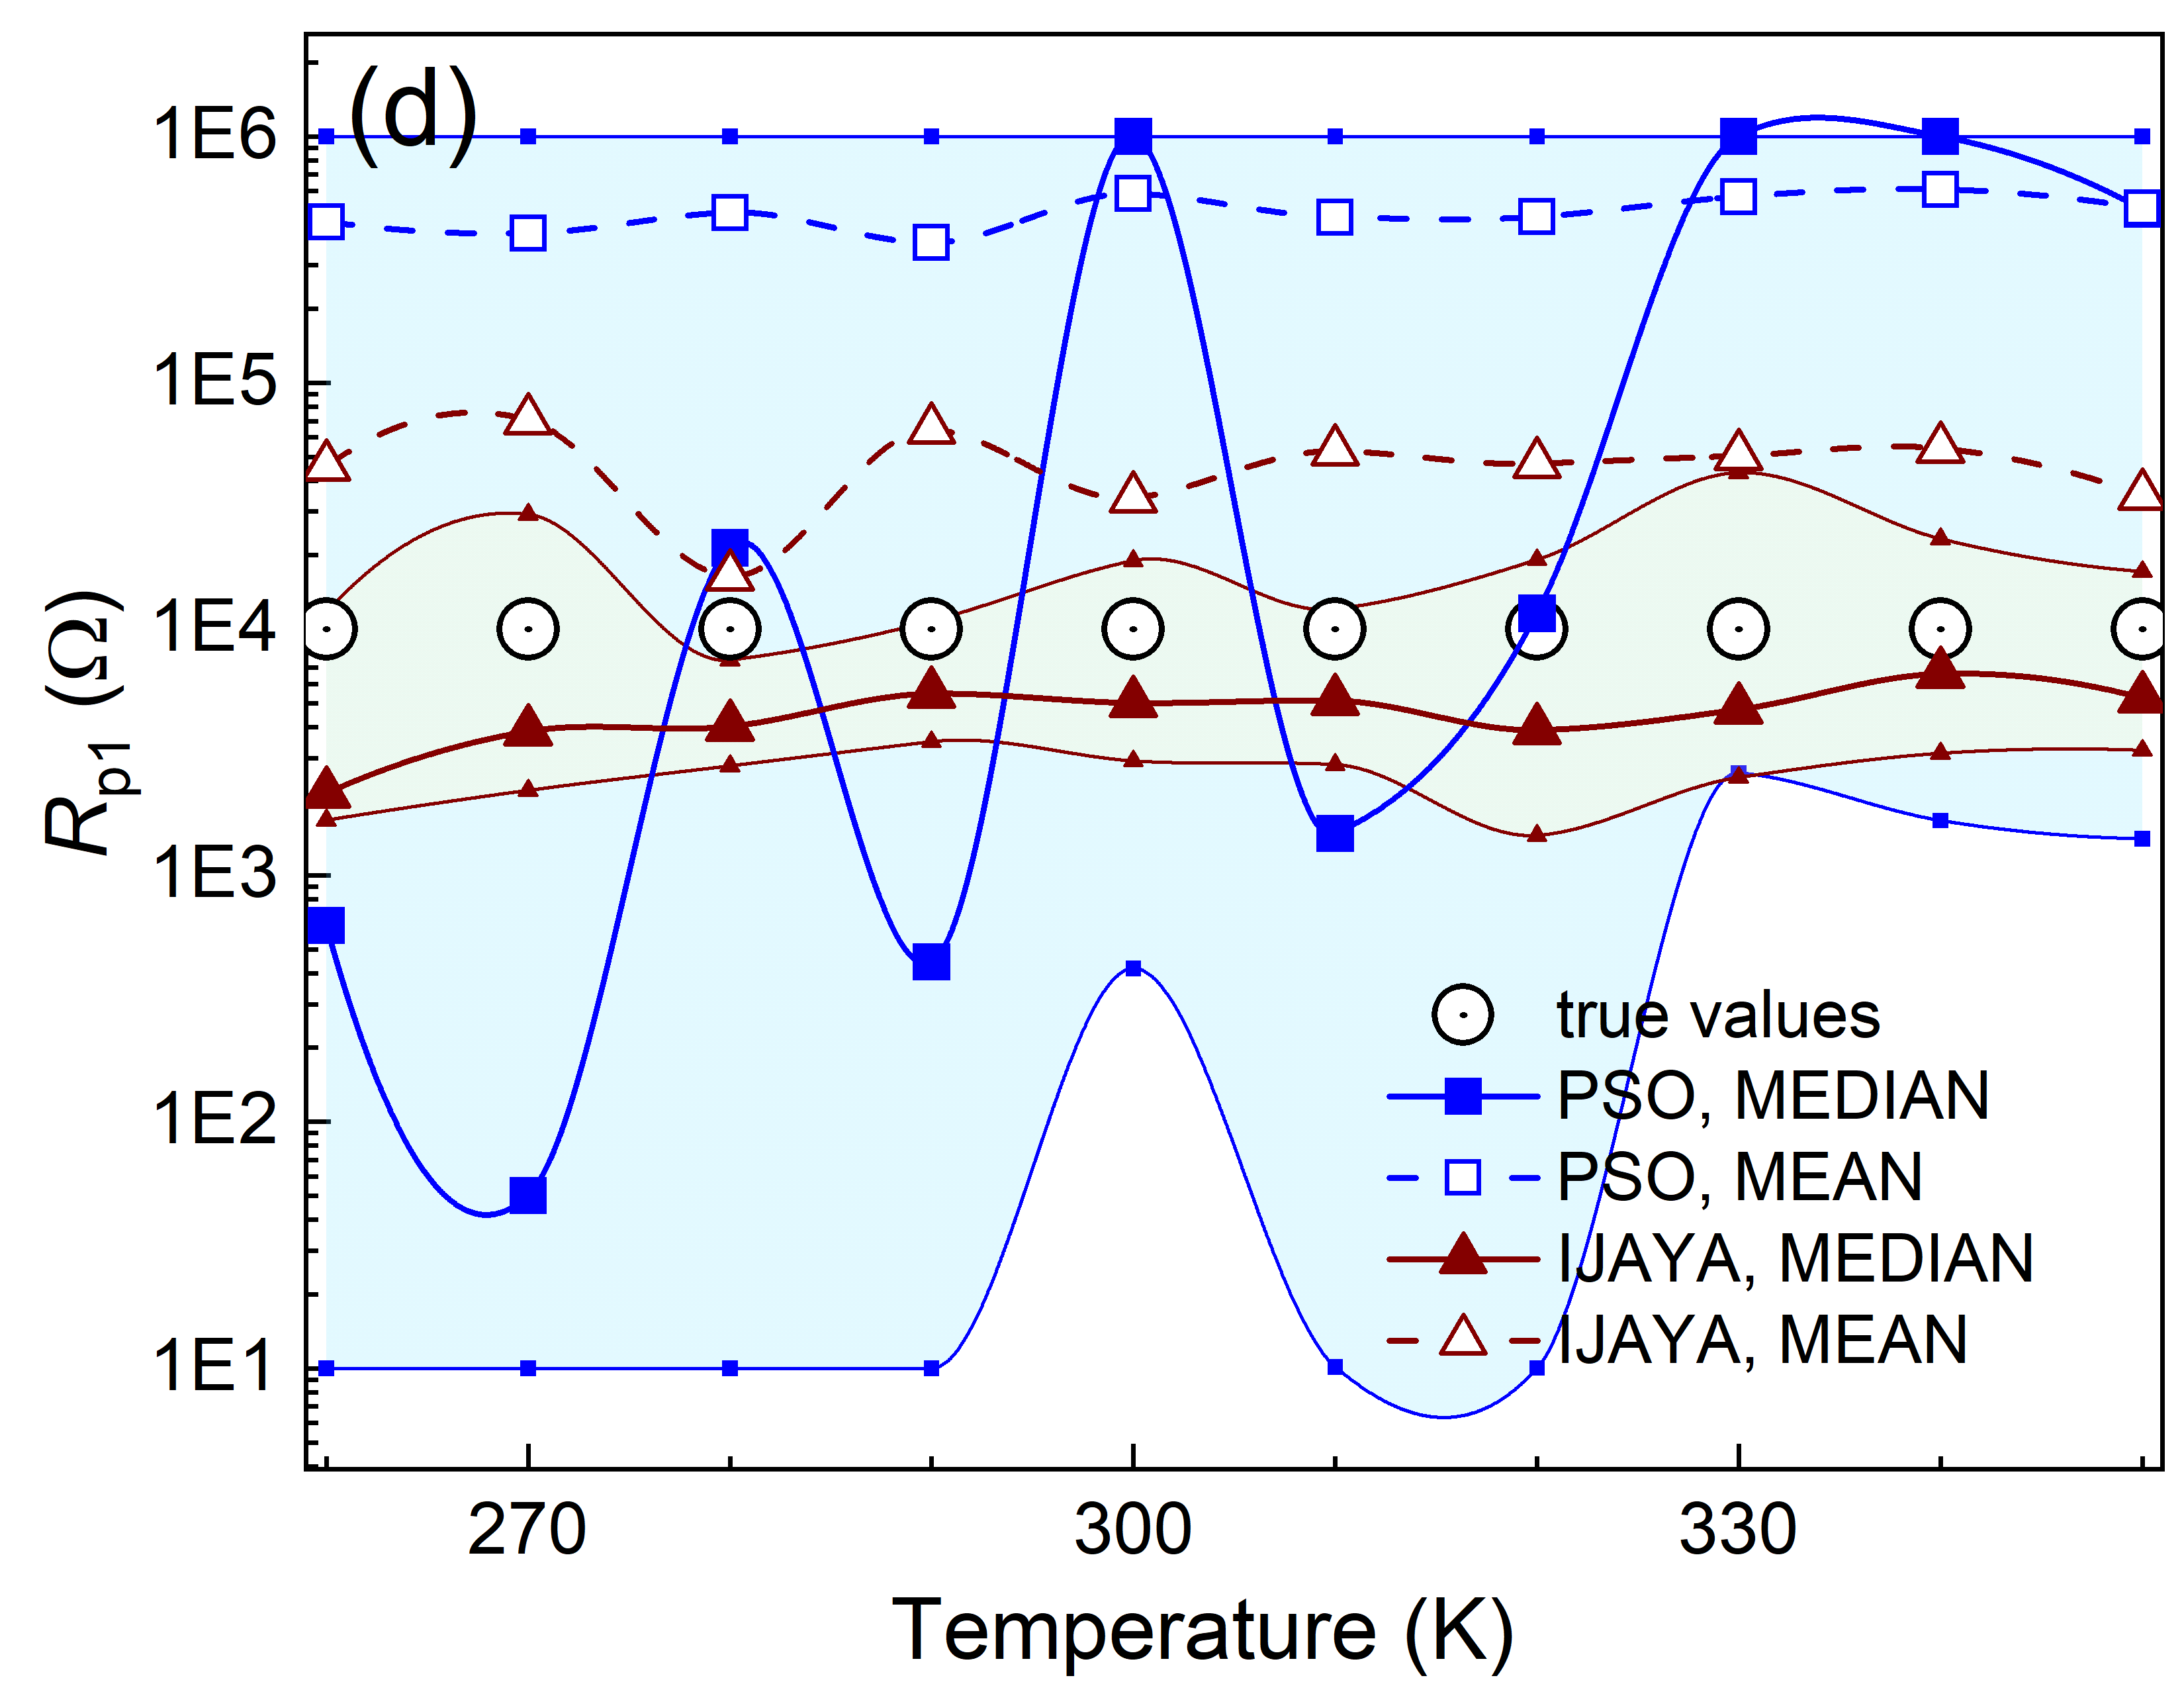
\includegraphics[width=.32\textwidth]{AfigD}
        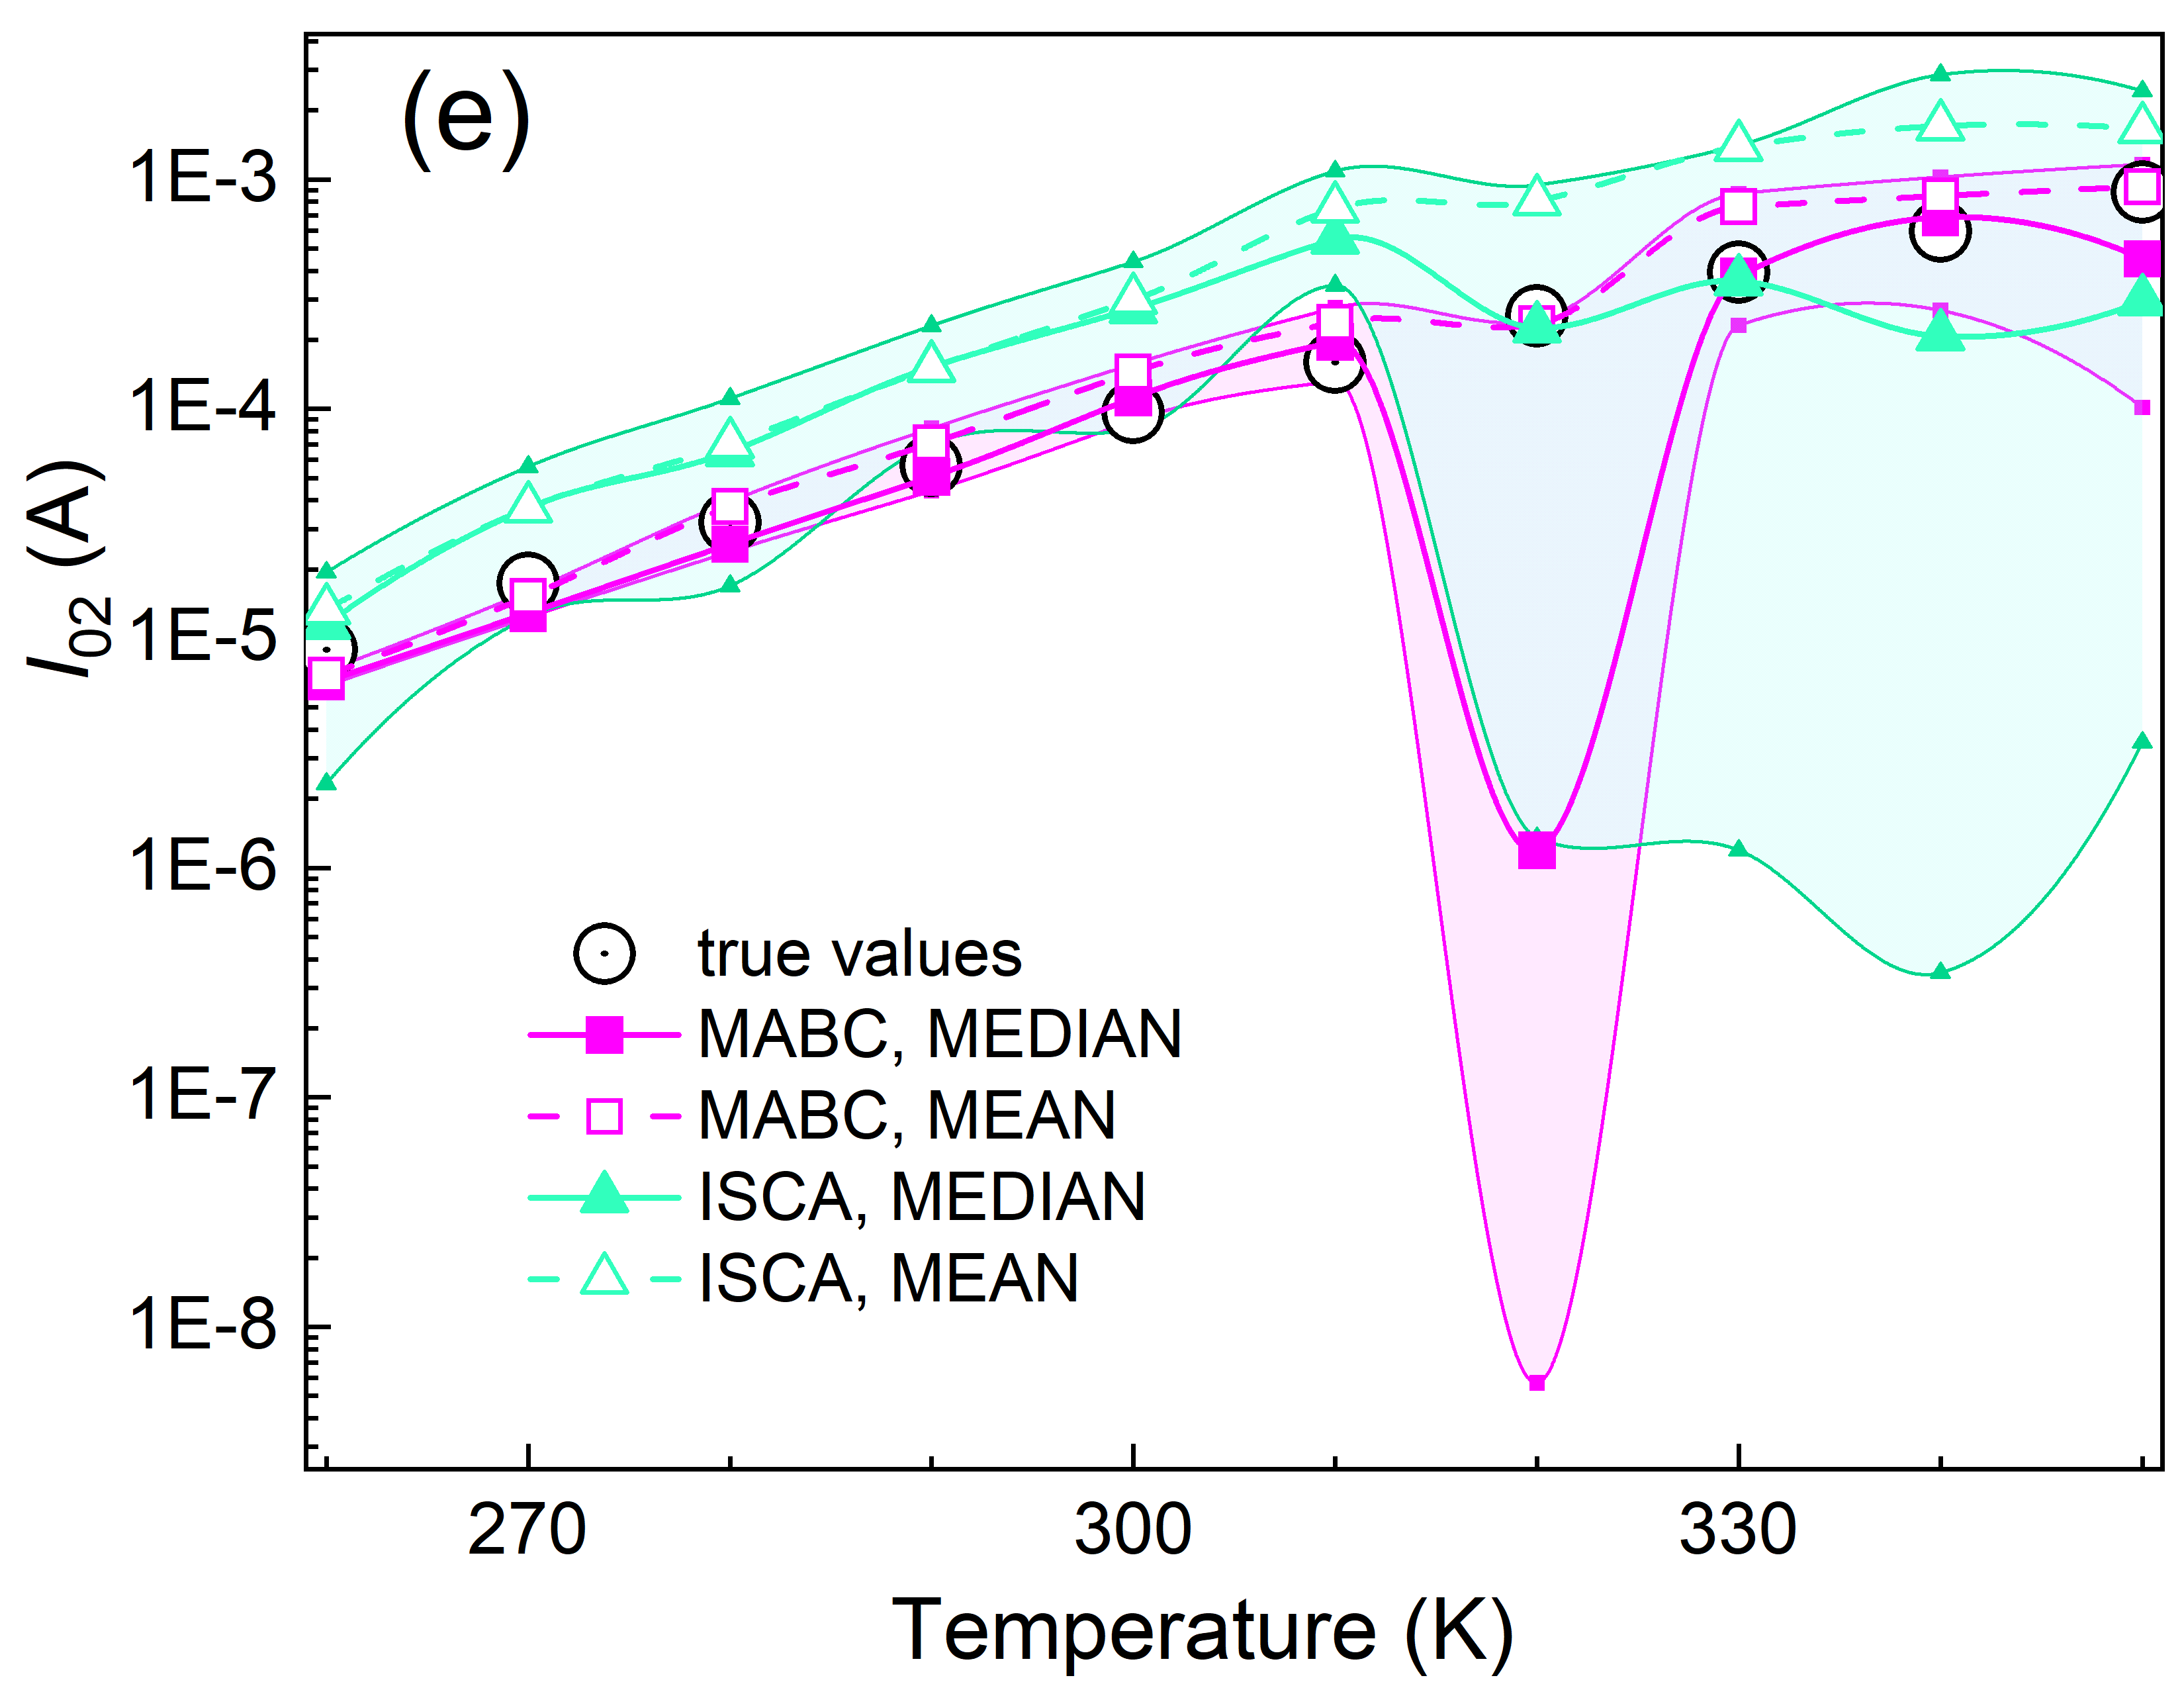
\includegraphics[width=.32\textwidth]{AfigE}
        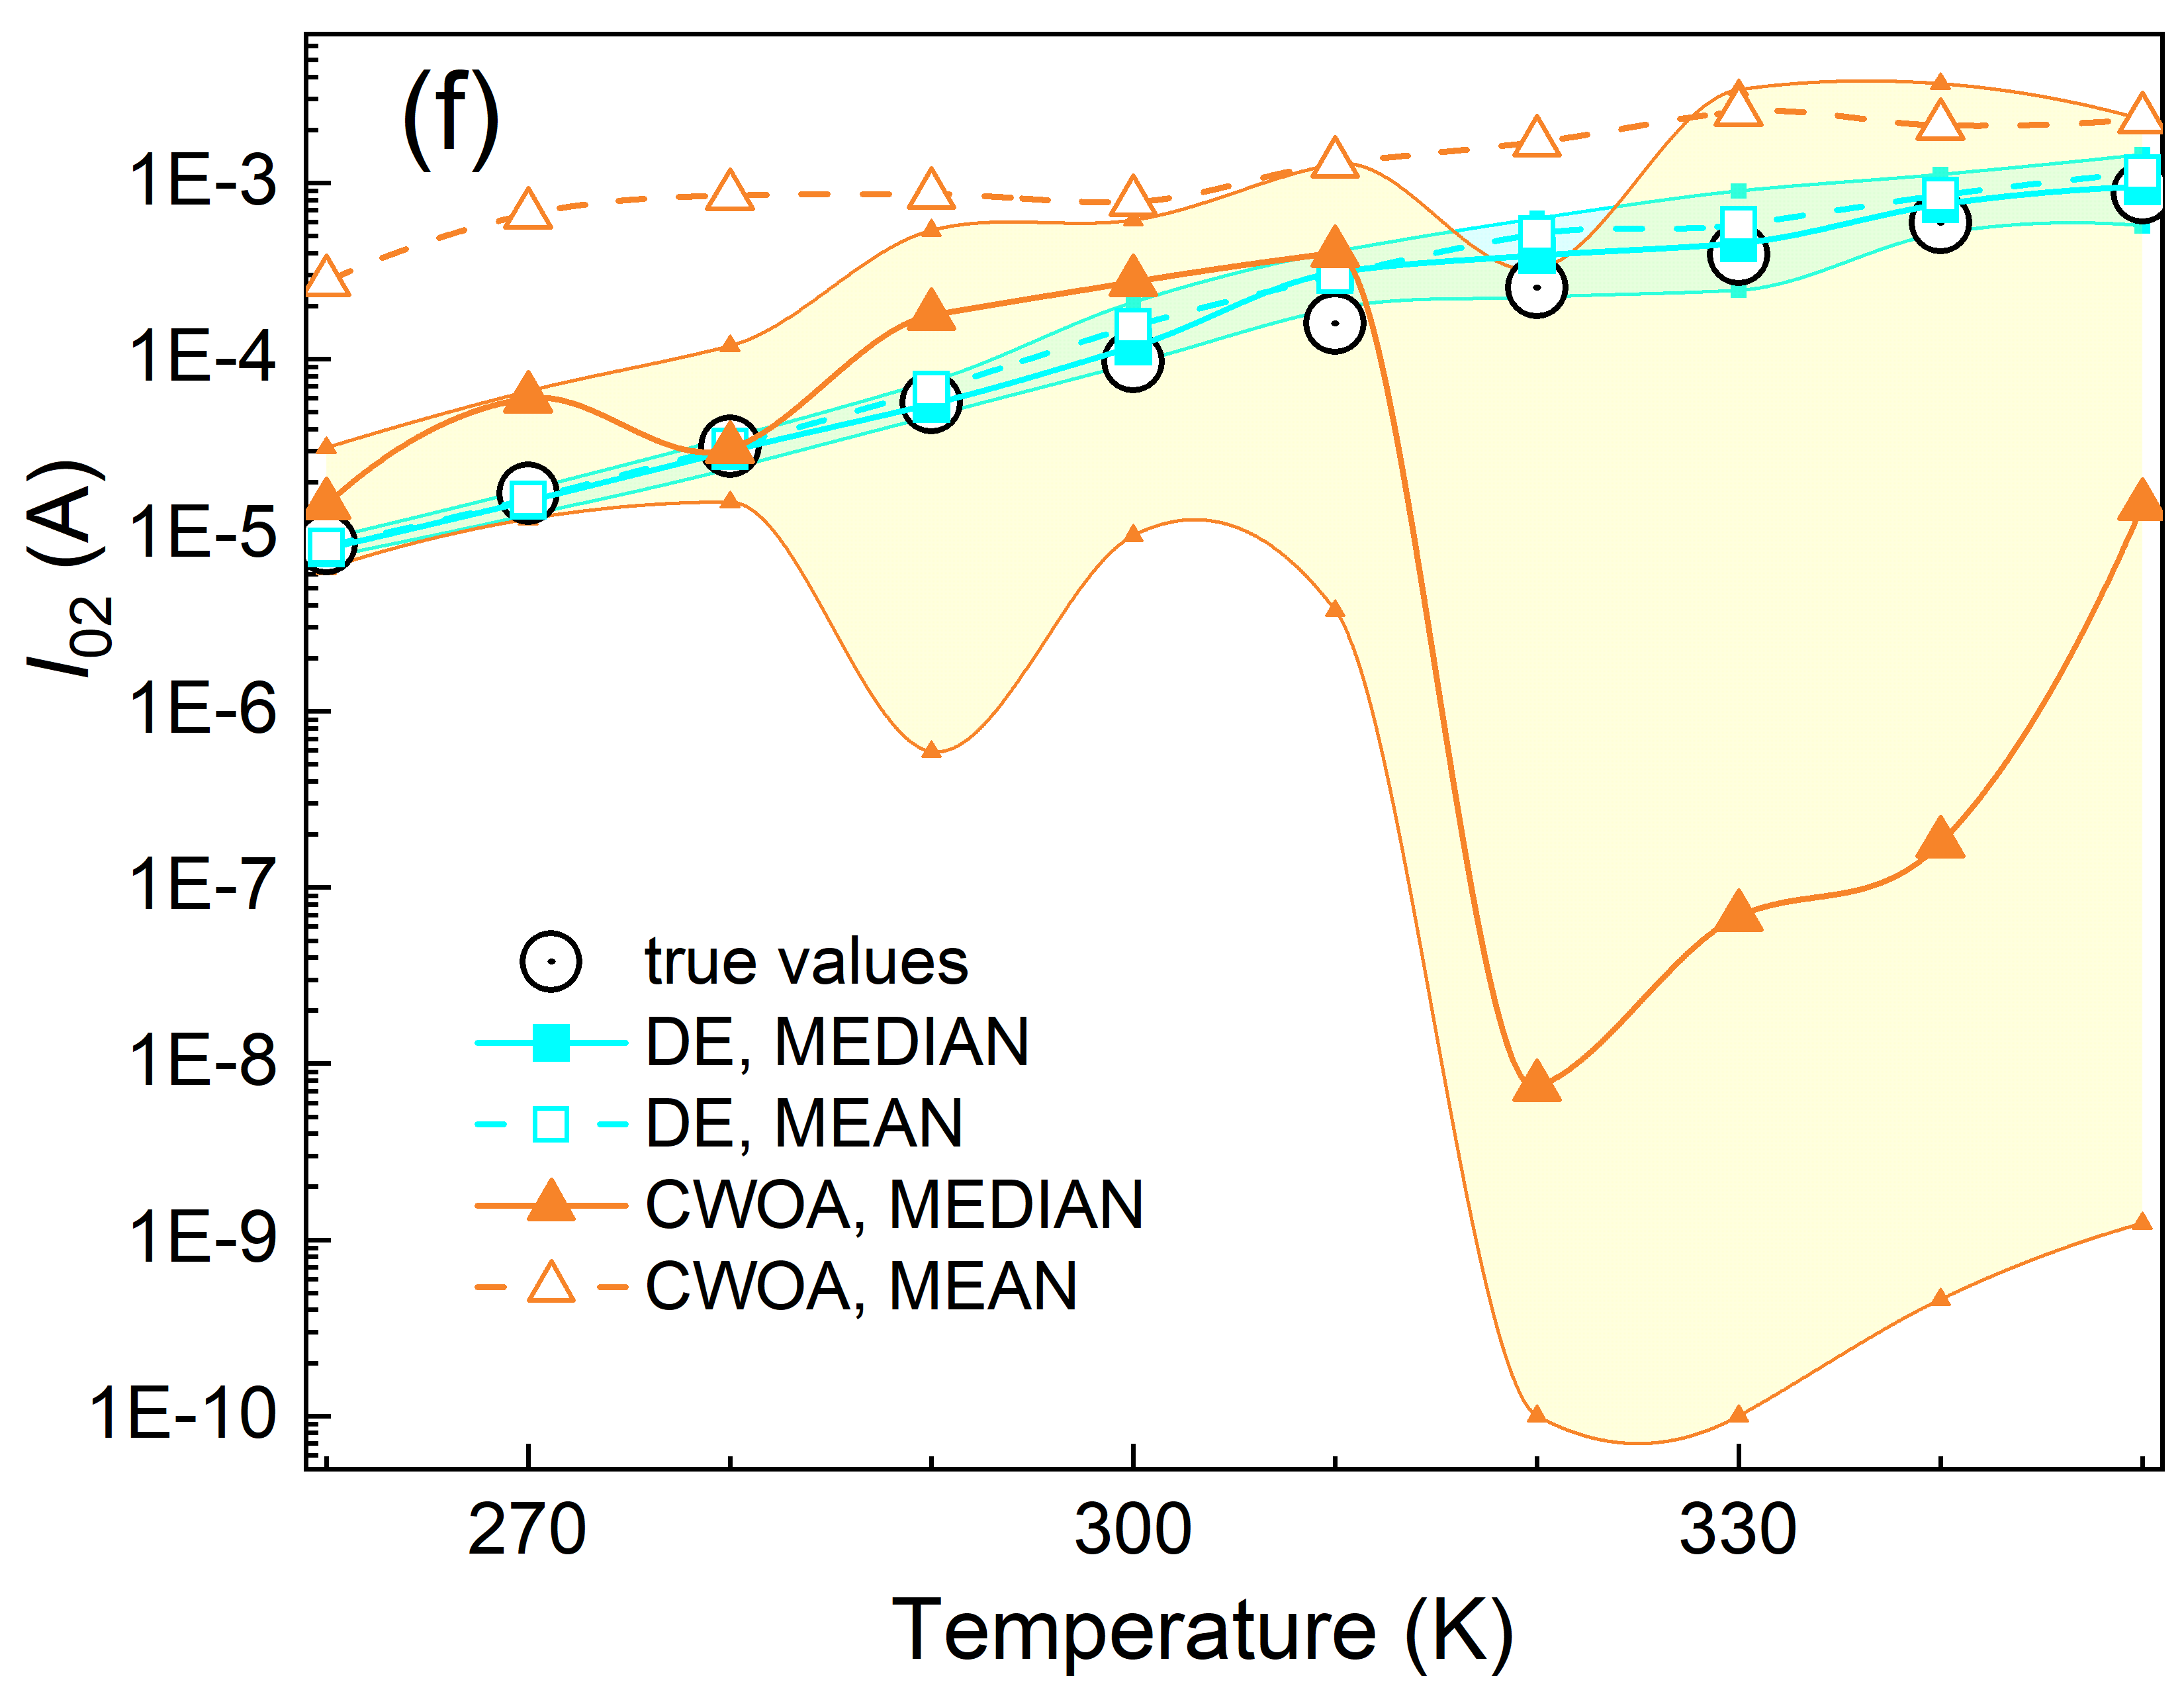
\includegraphics[width=.32\textwidth]{AfigF}
		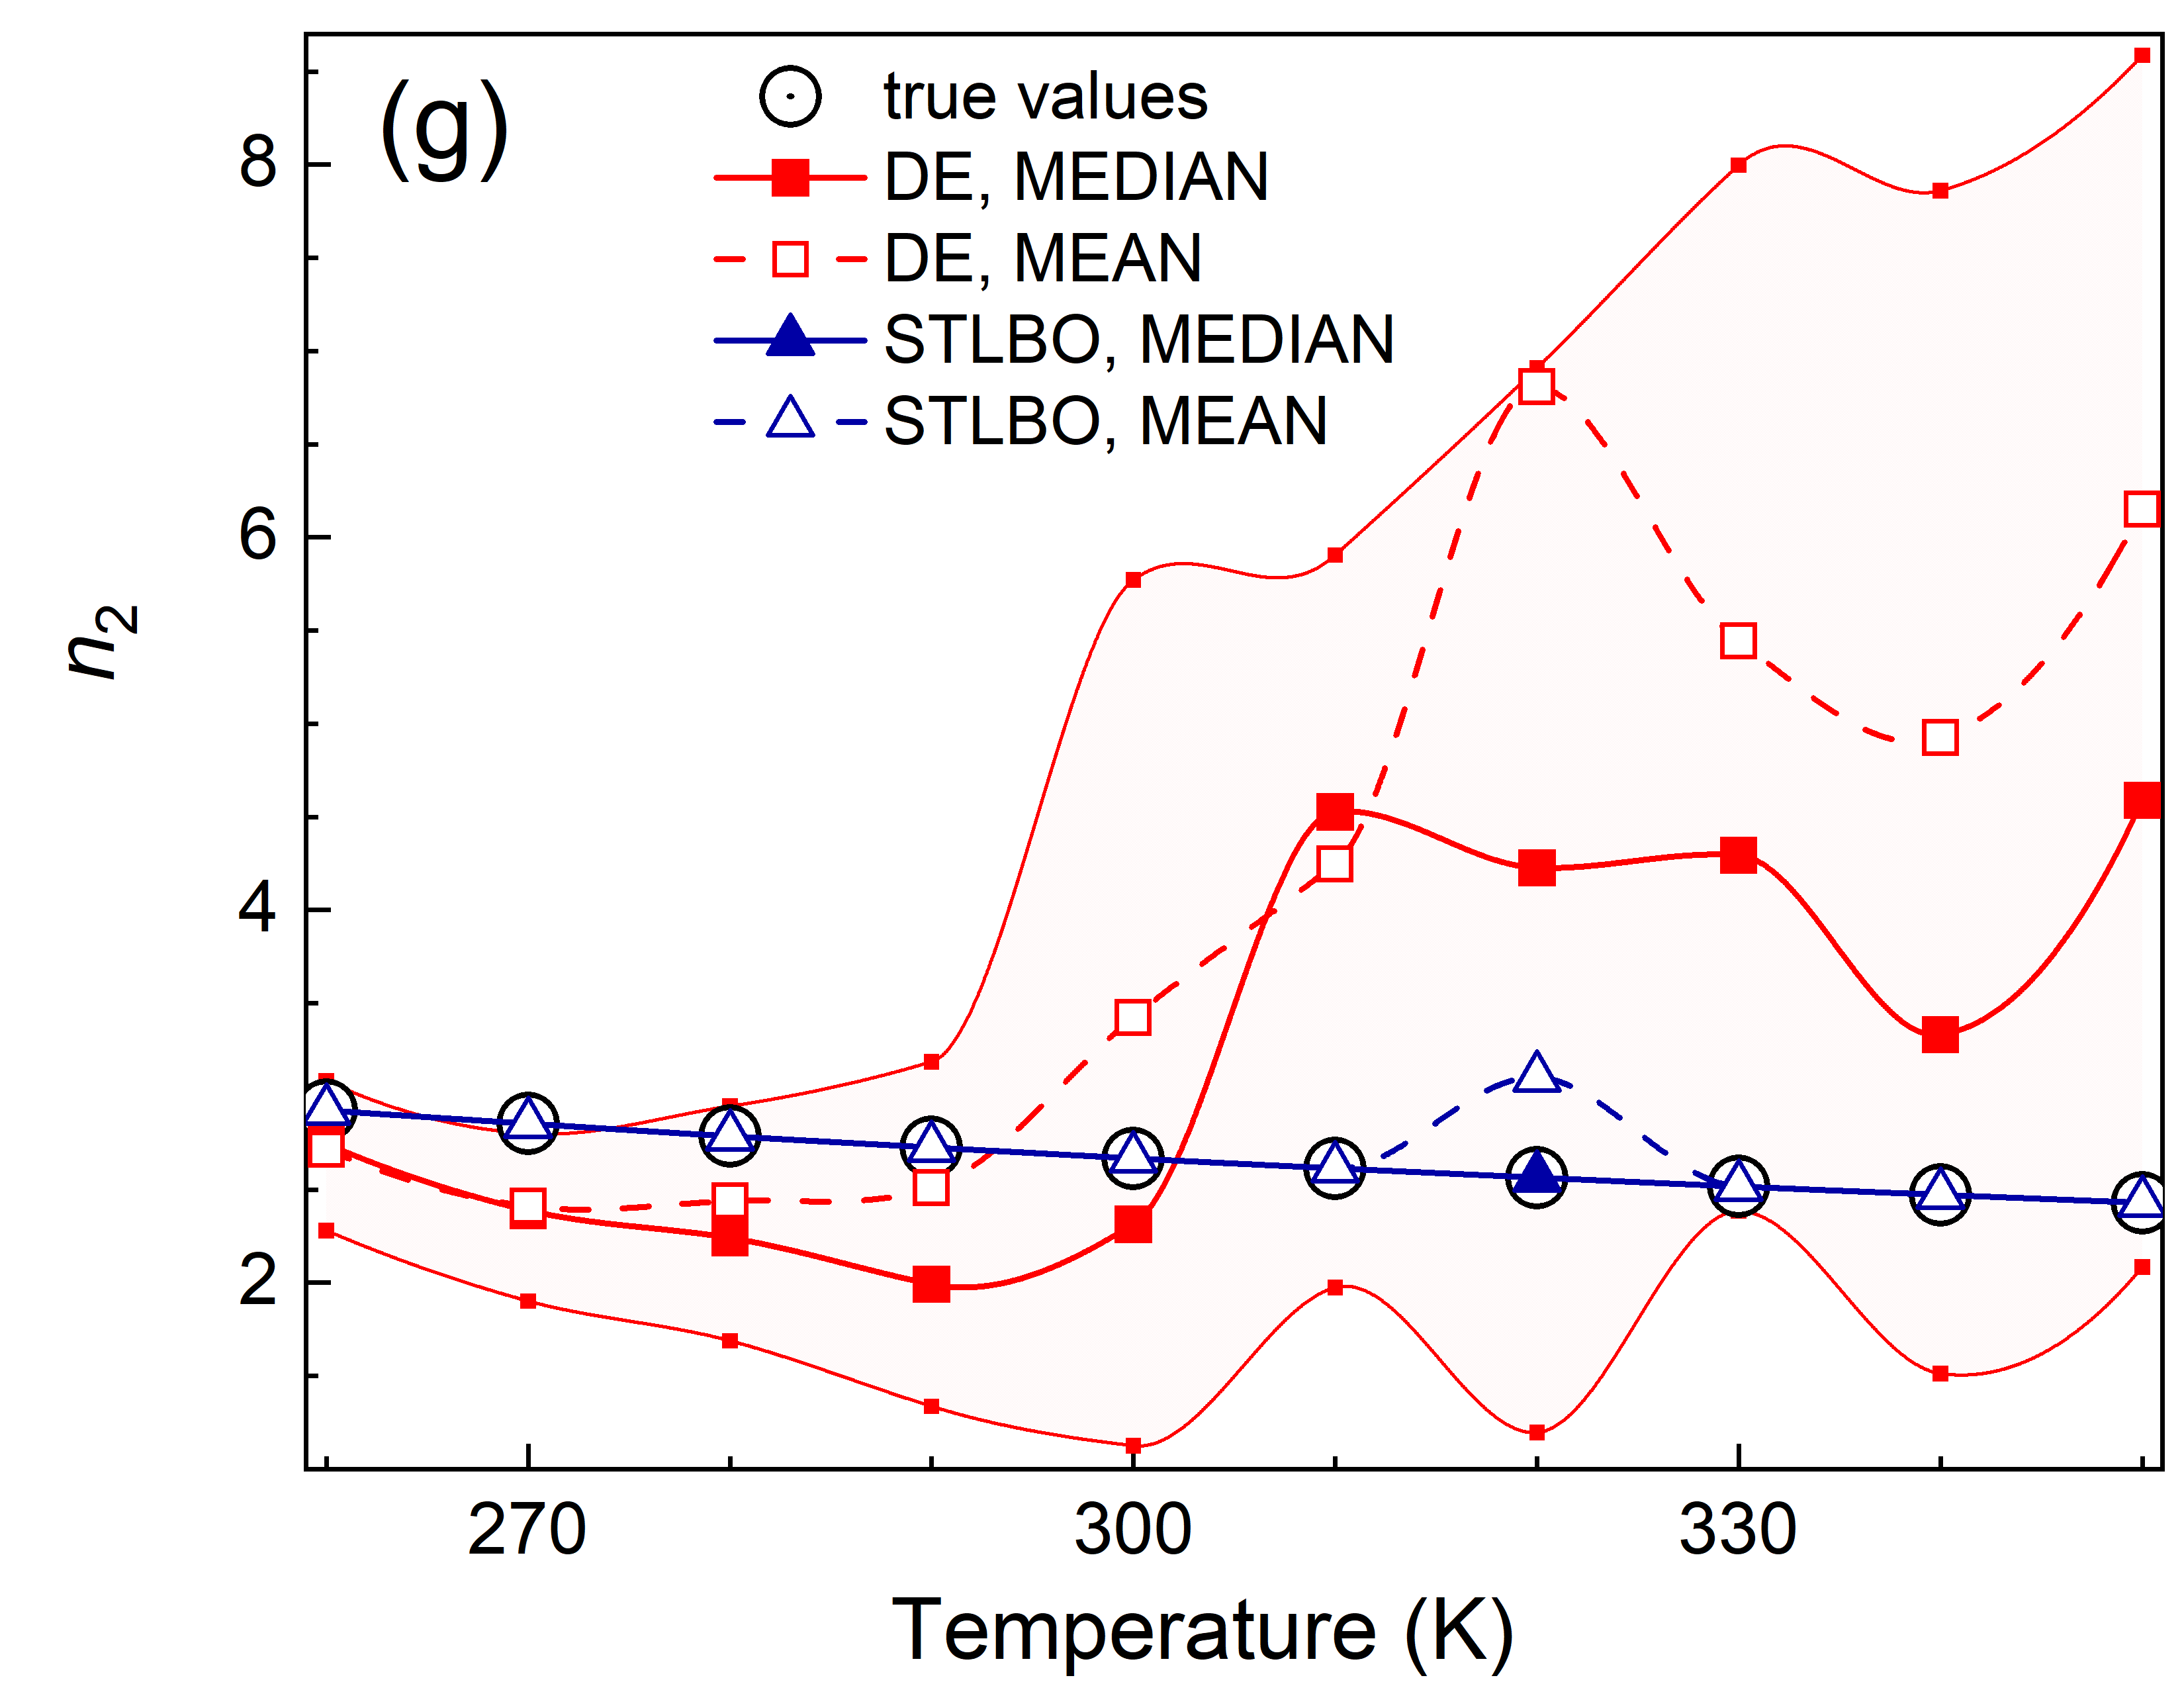
\includegraphics[width=.32\textwidth]{AfigG}
        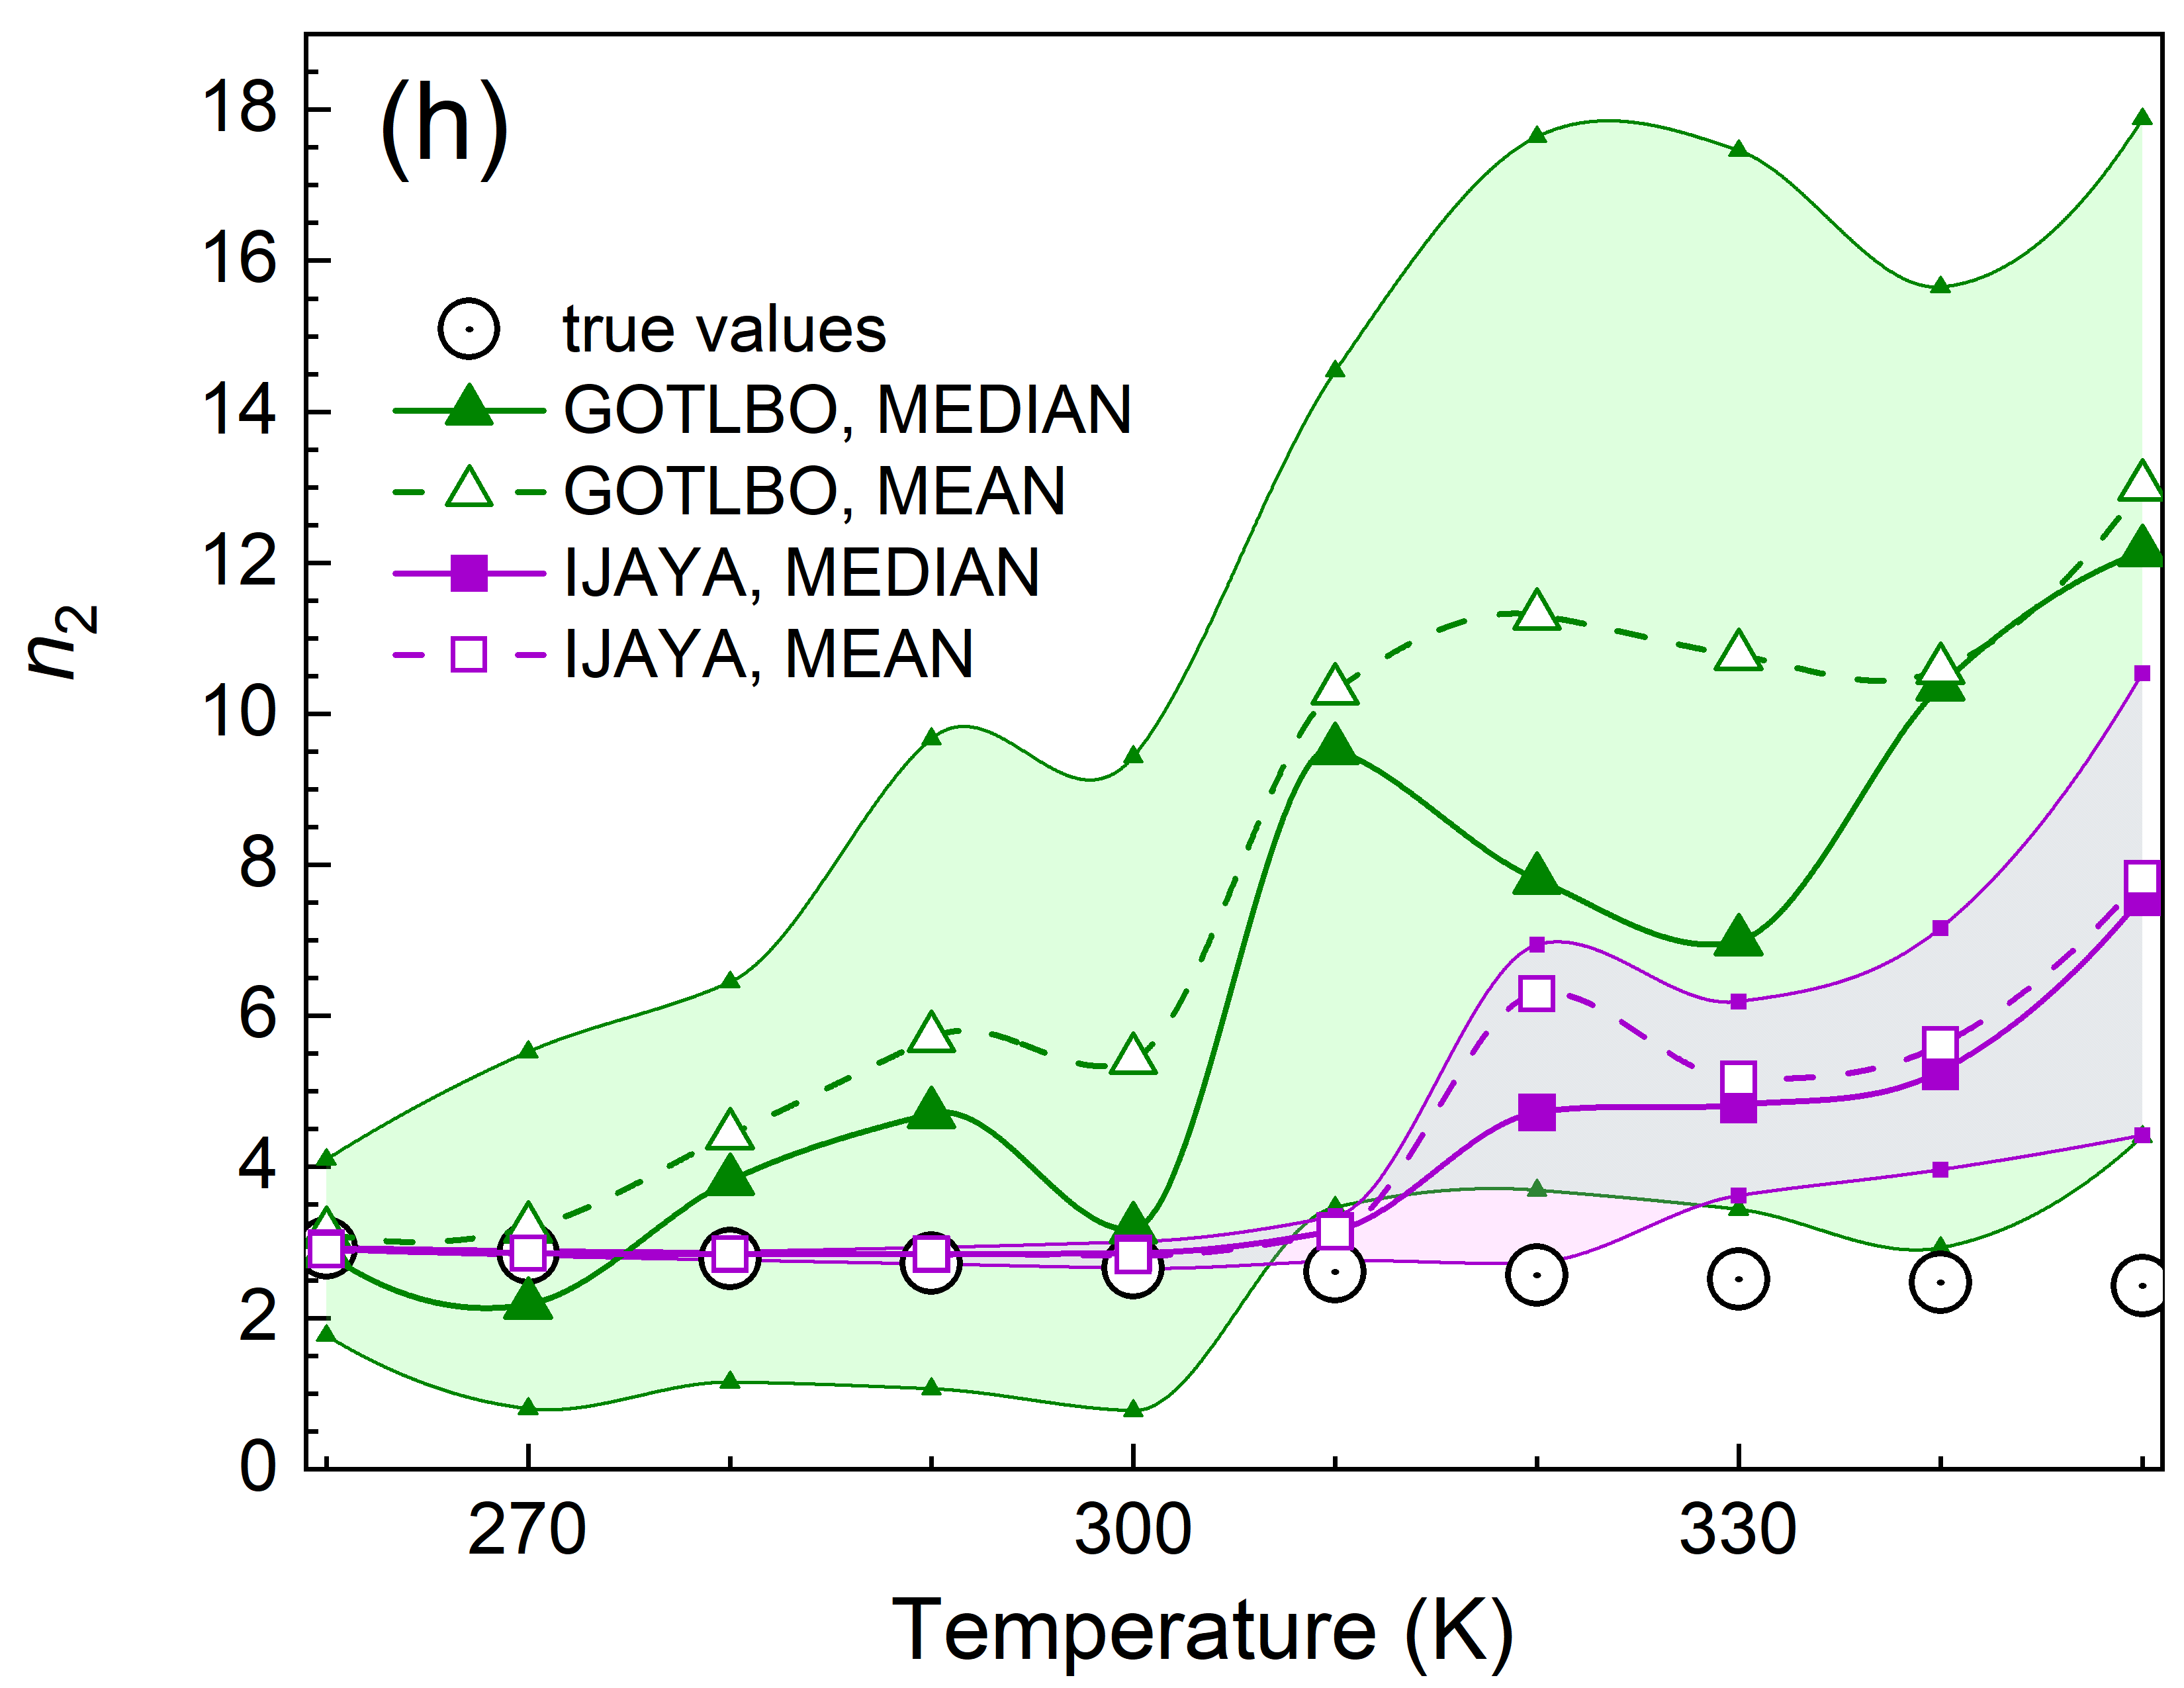
\includegraphics[width=.32\textwidth]{AfigH}
        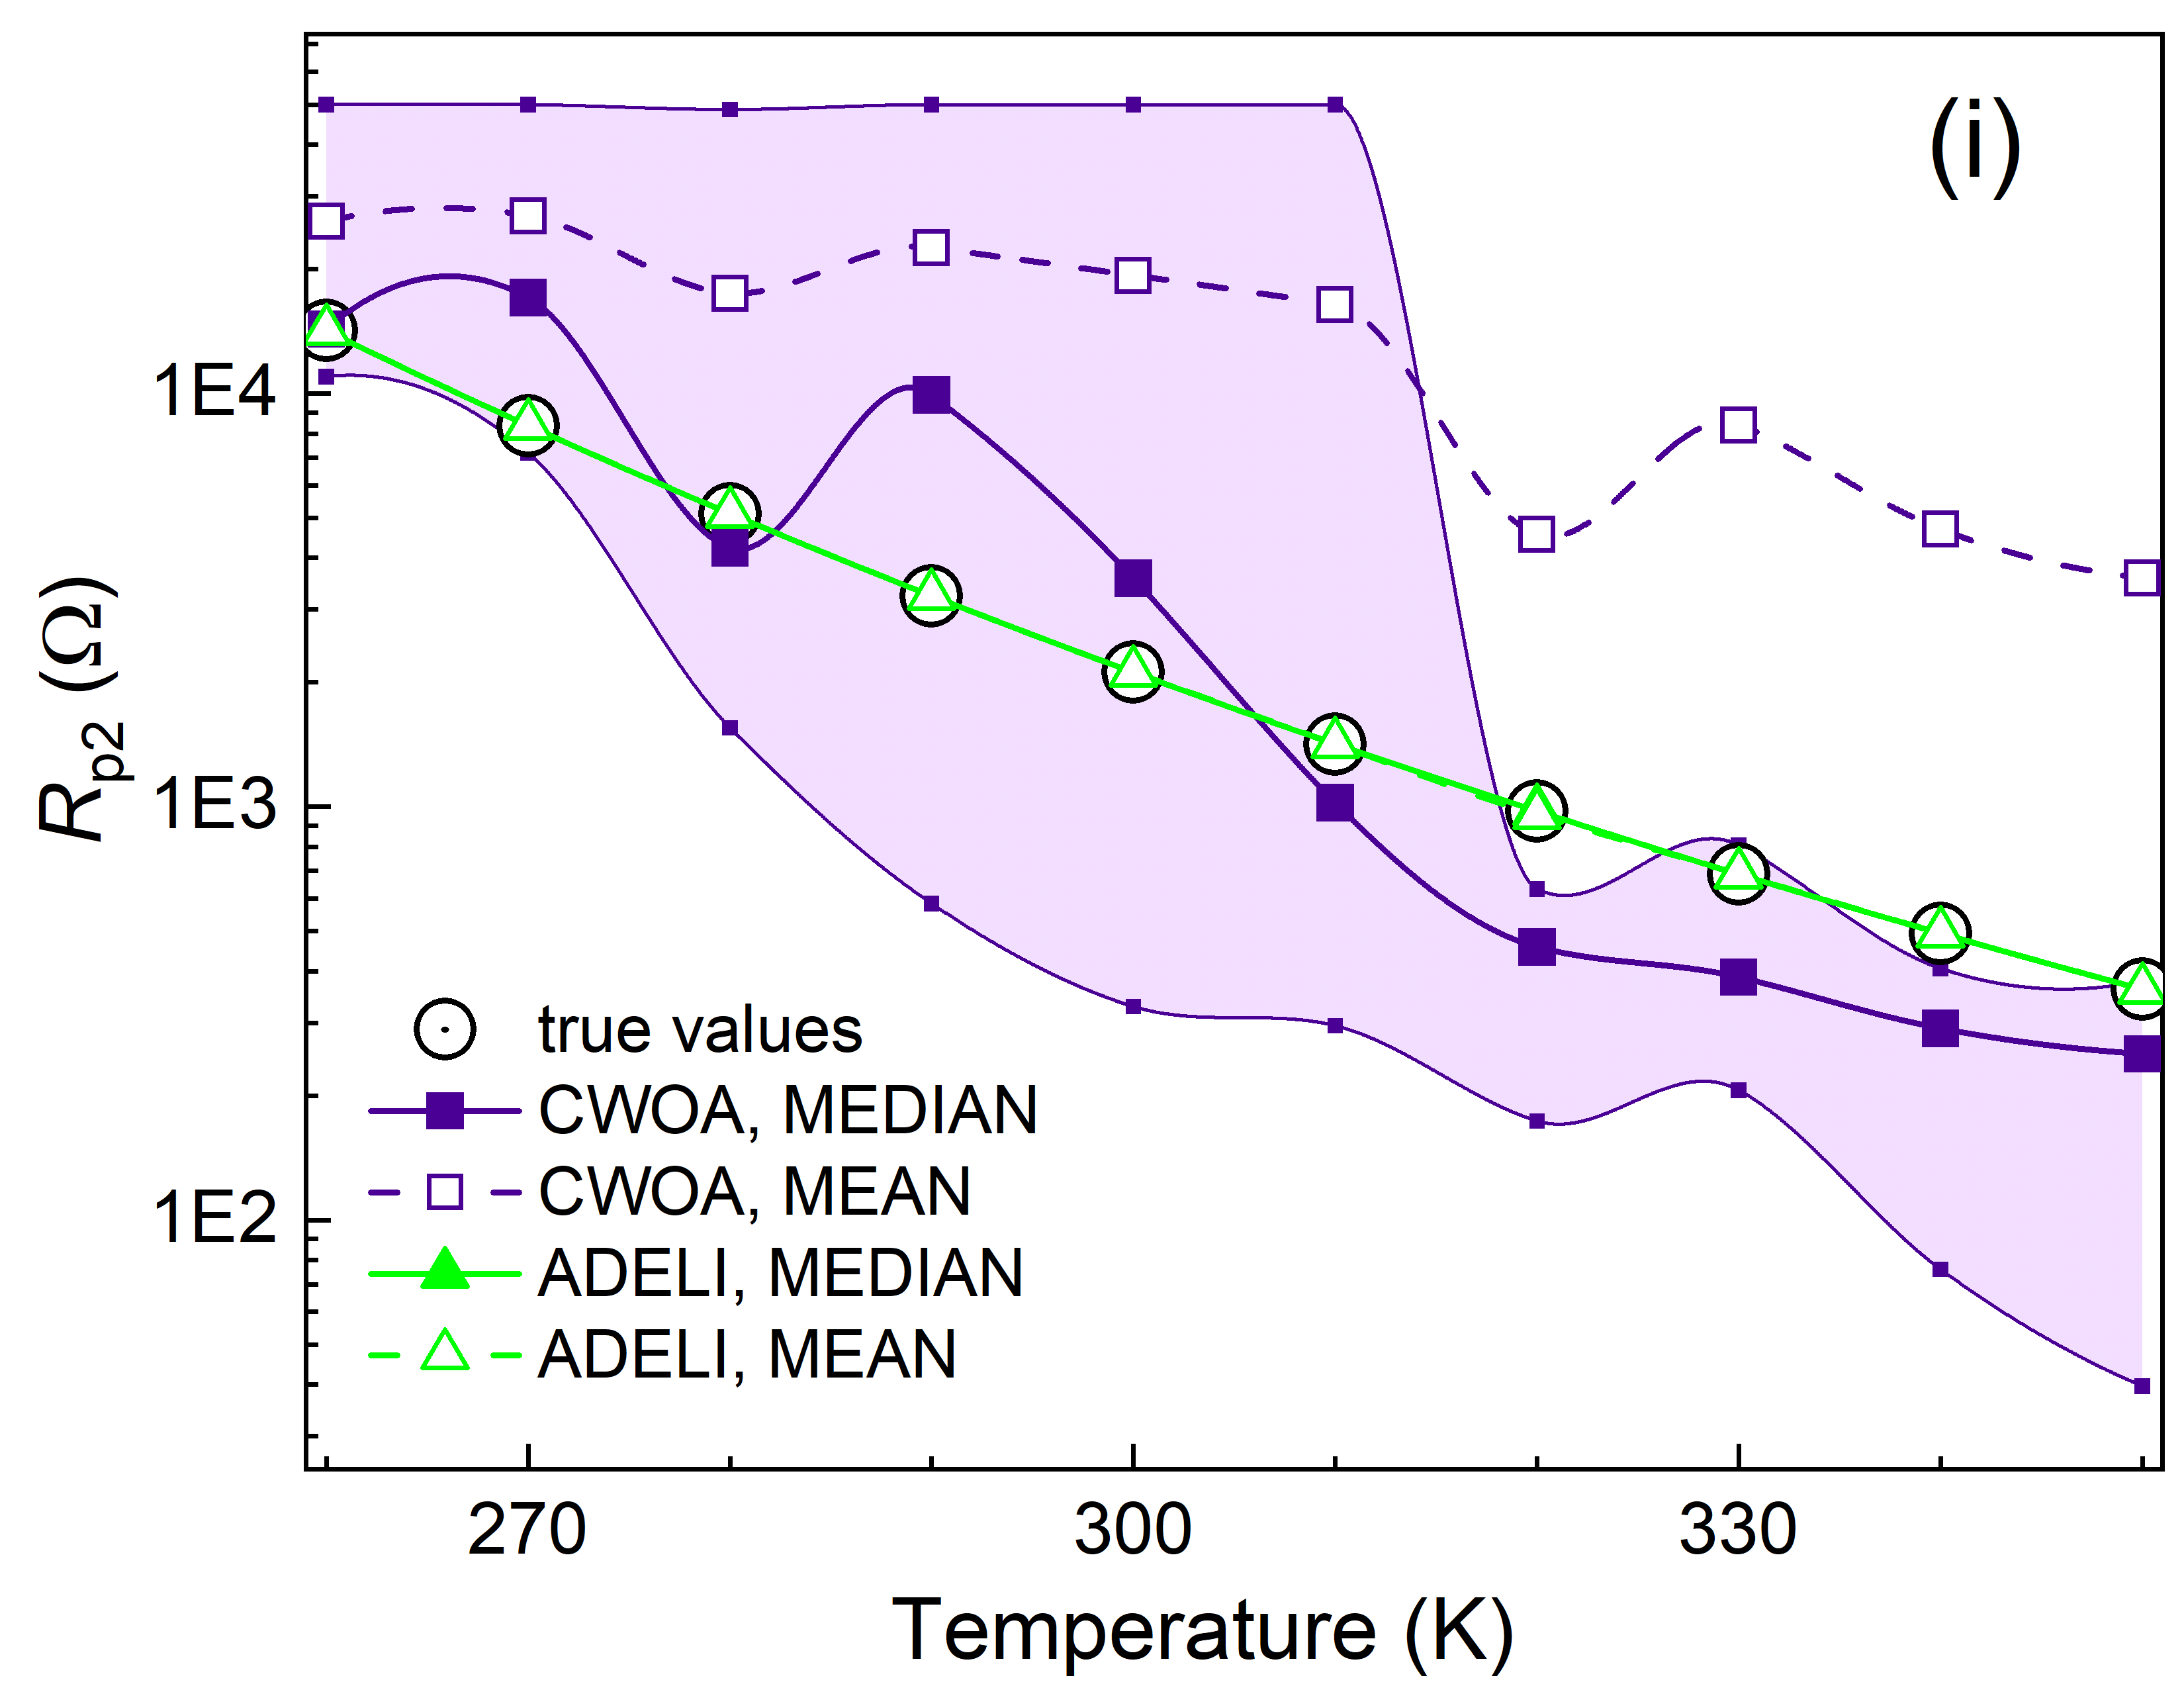
\includegraphics[width=.32\textwidth]{AfigI}
		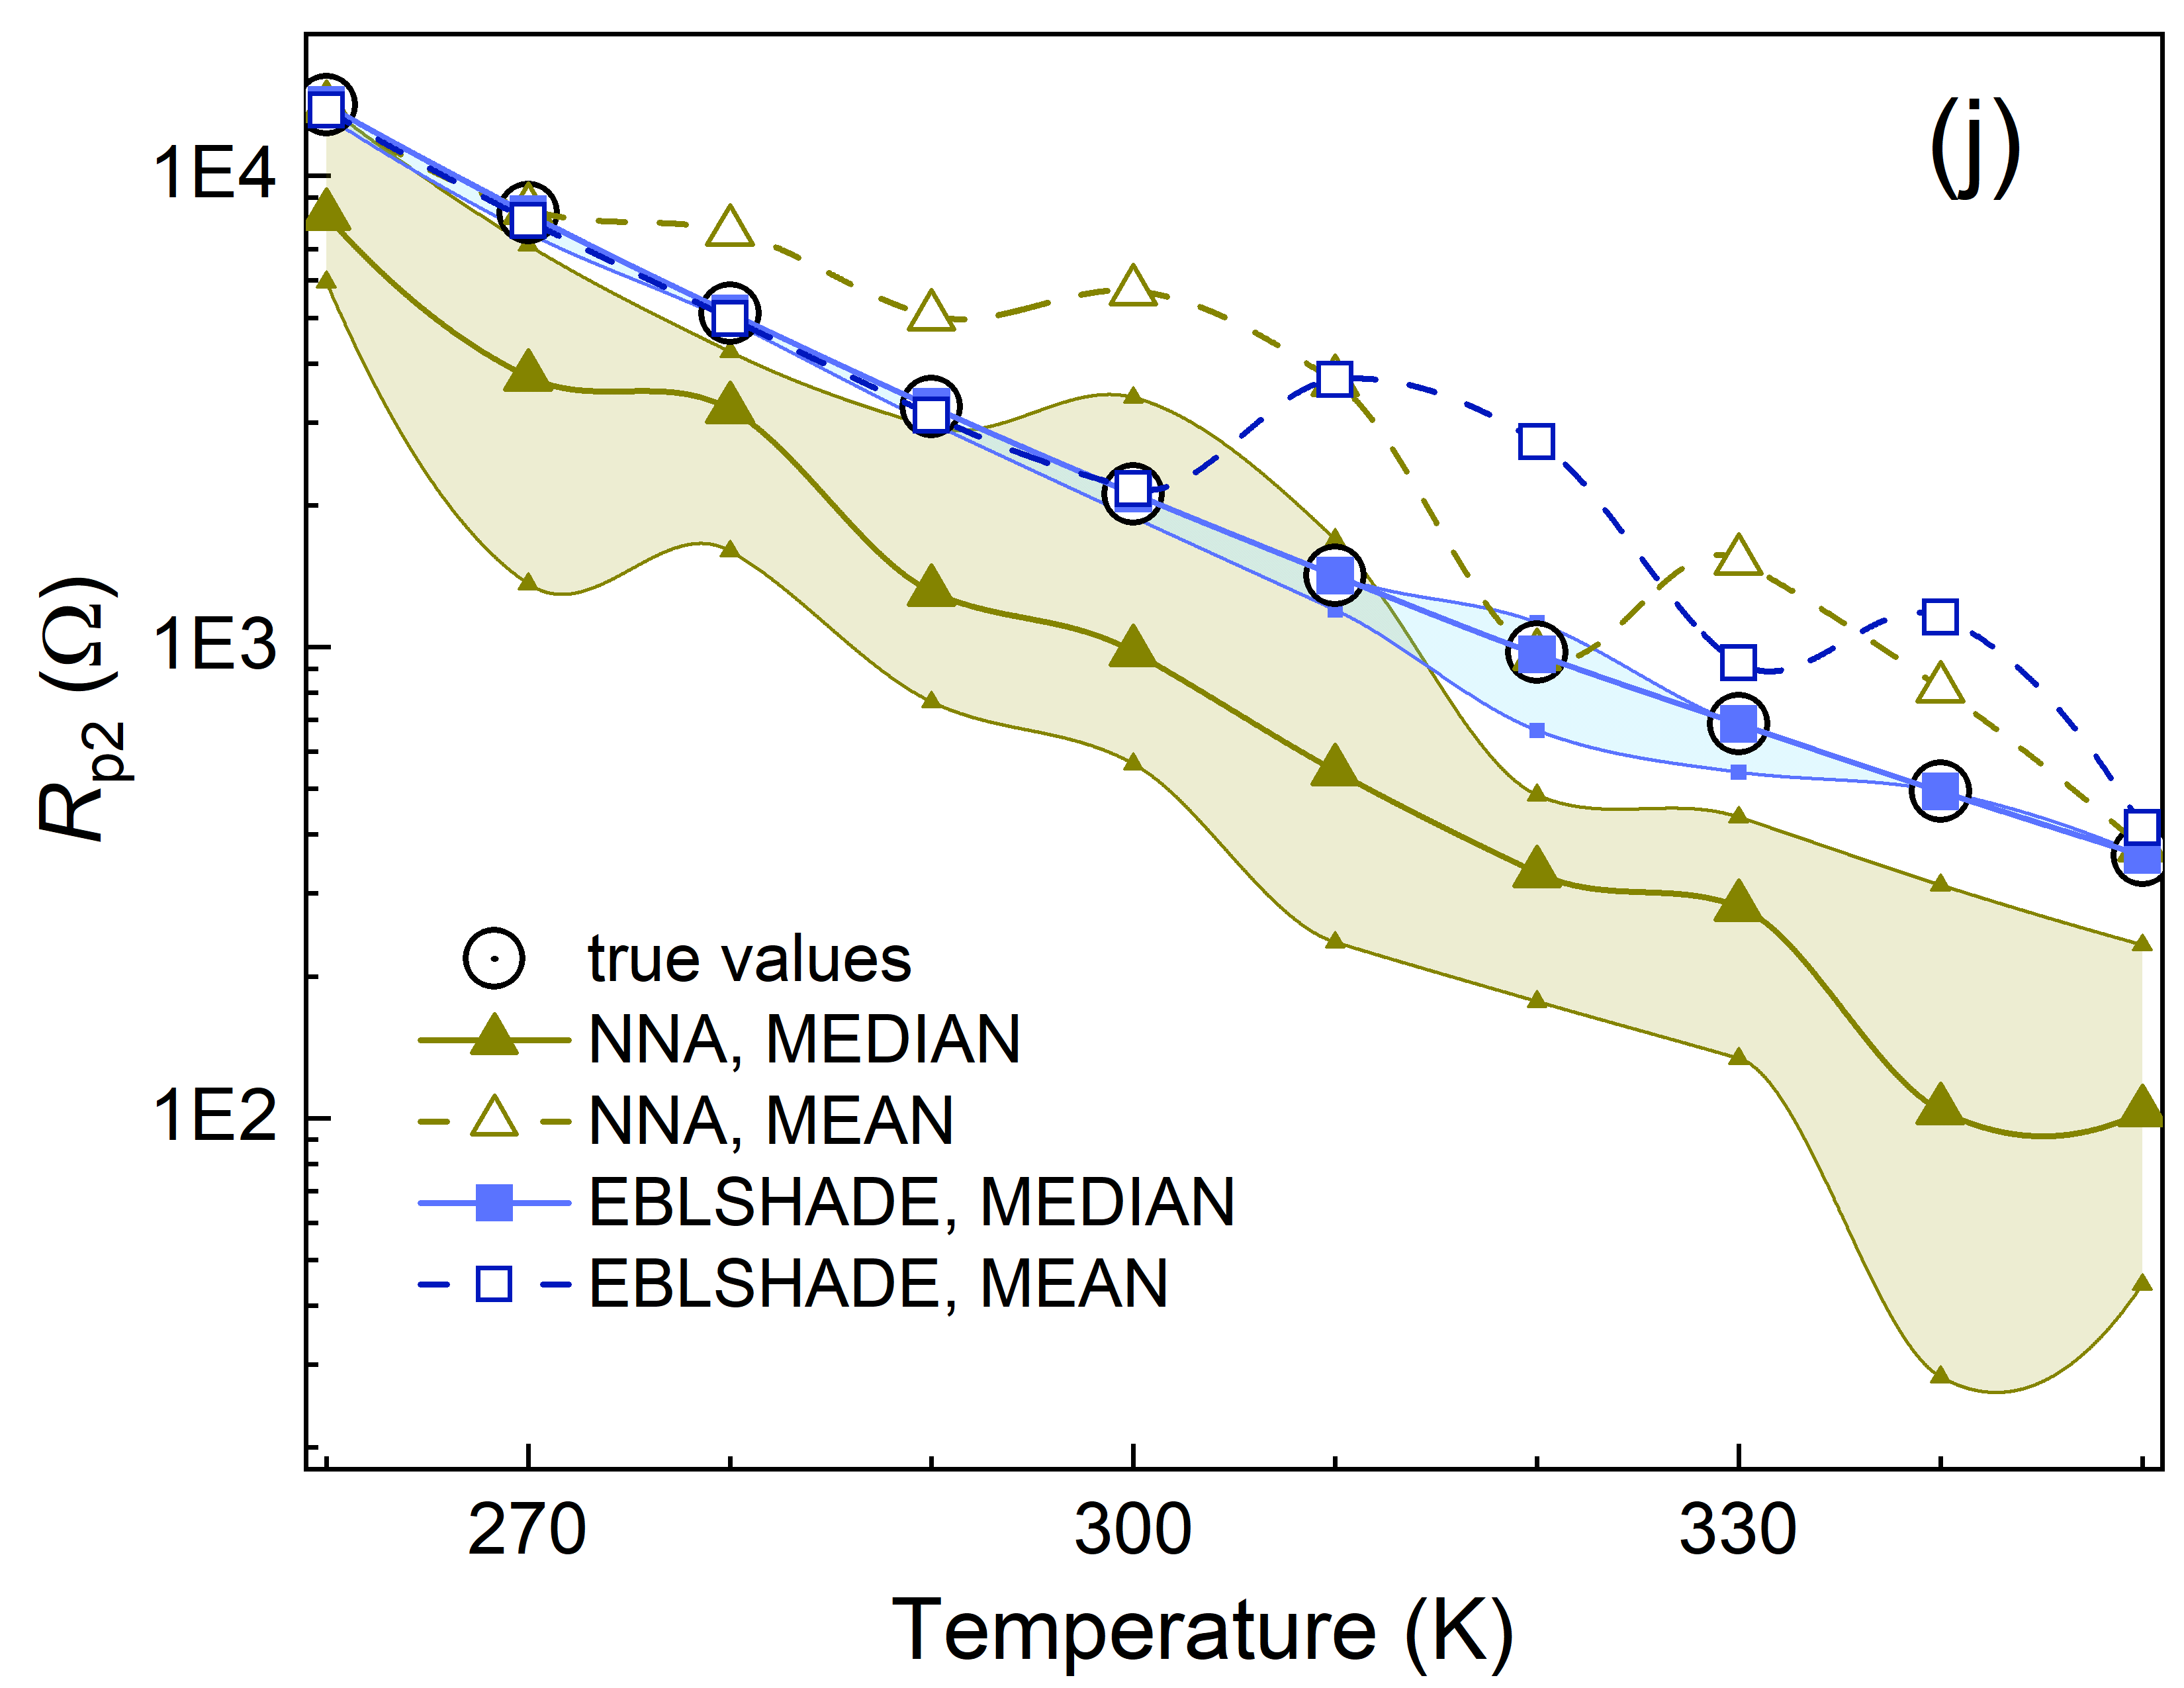
\includegraphics[width=.32\textwidth]{AfigJ}
        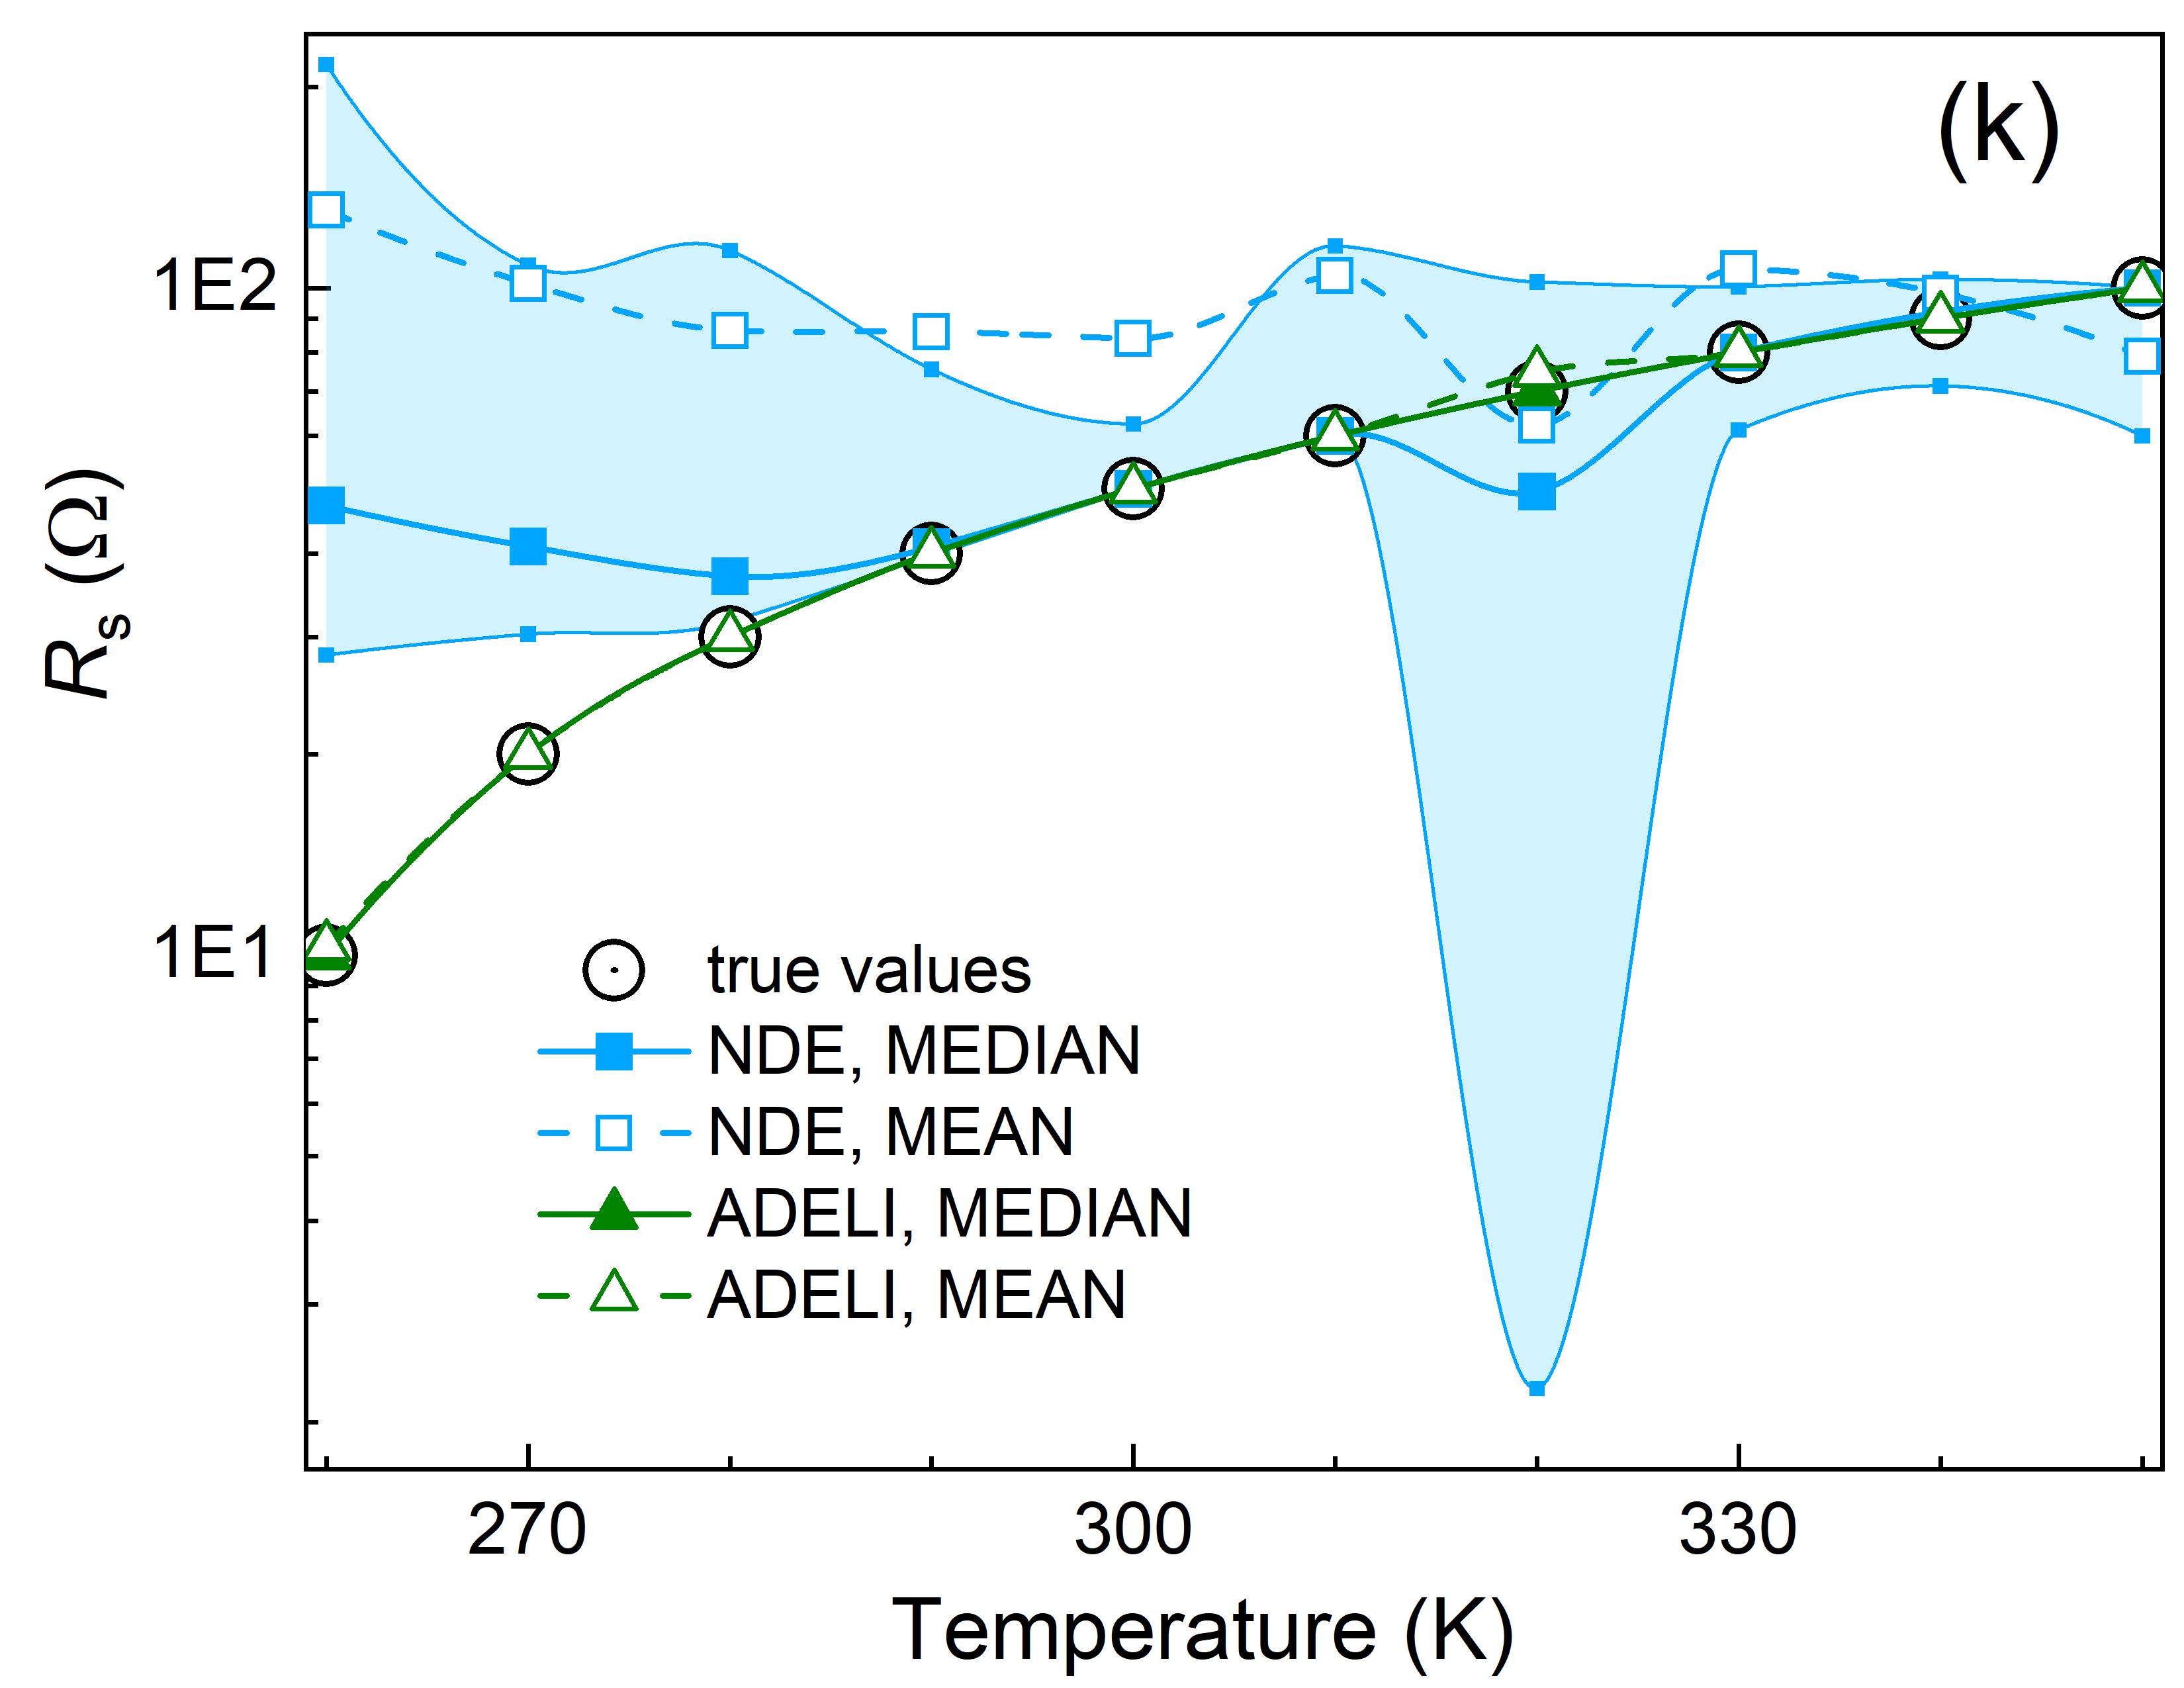
\includegraphics[width=.32\textwidth]{AfigK}
        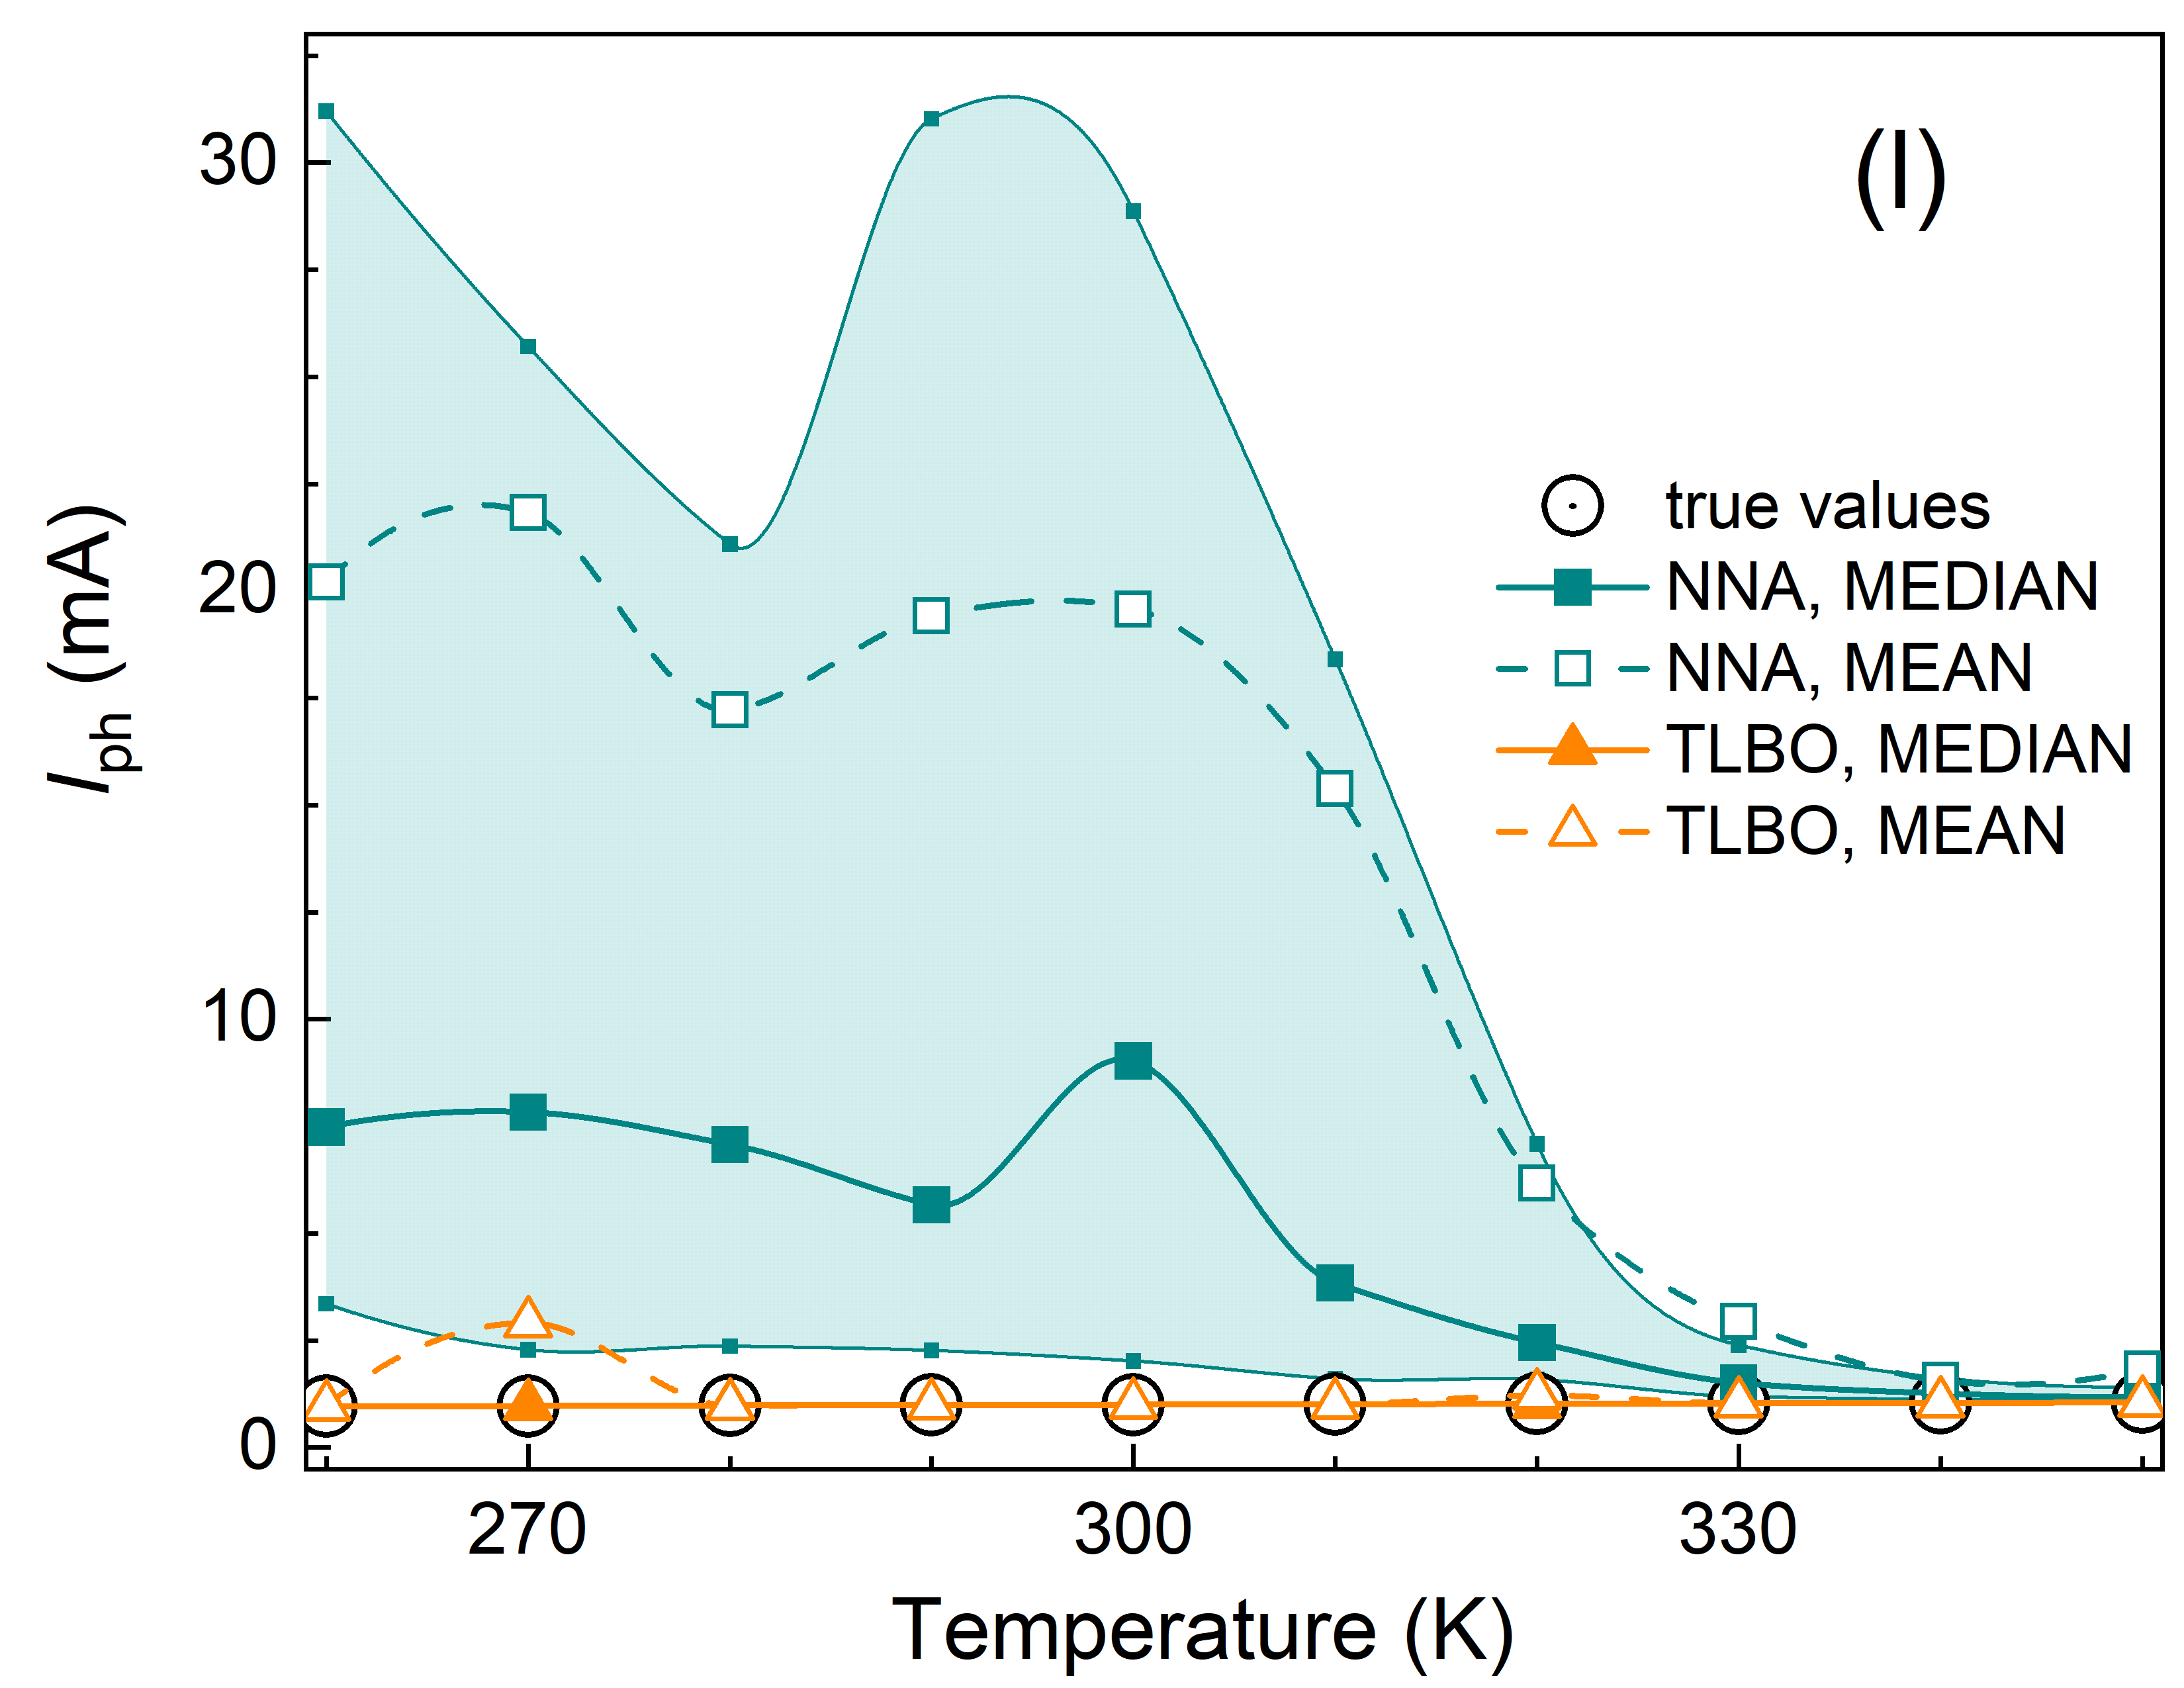
\includegraphics[width=.32\textwidth]{AfigL}
		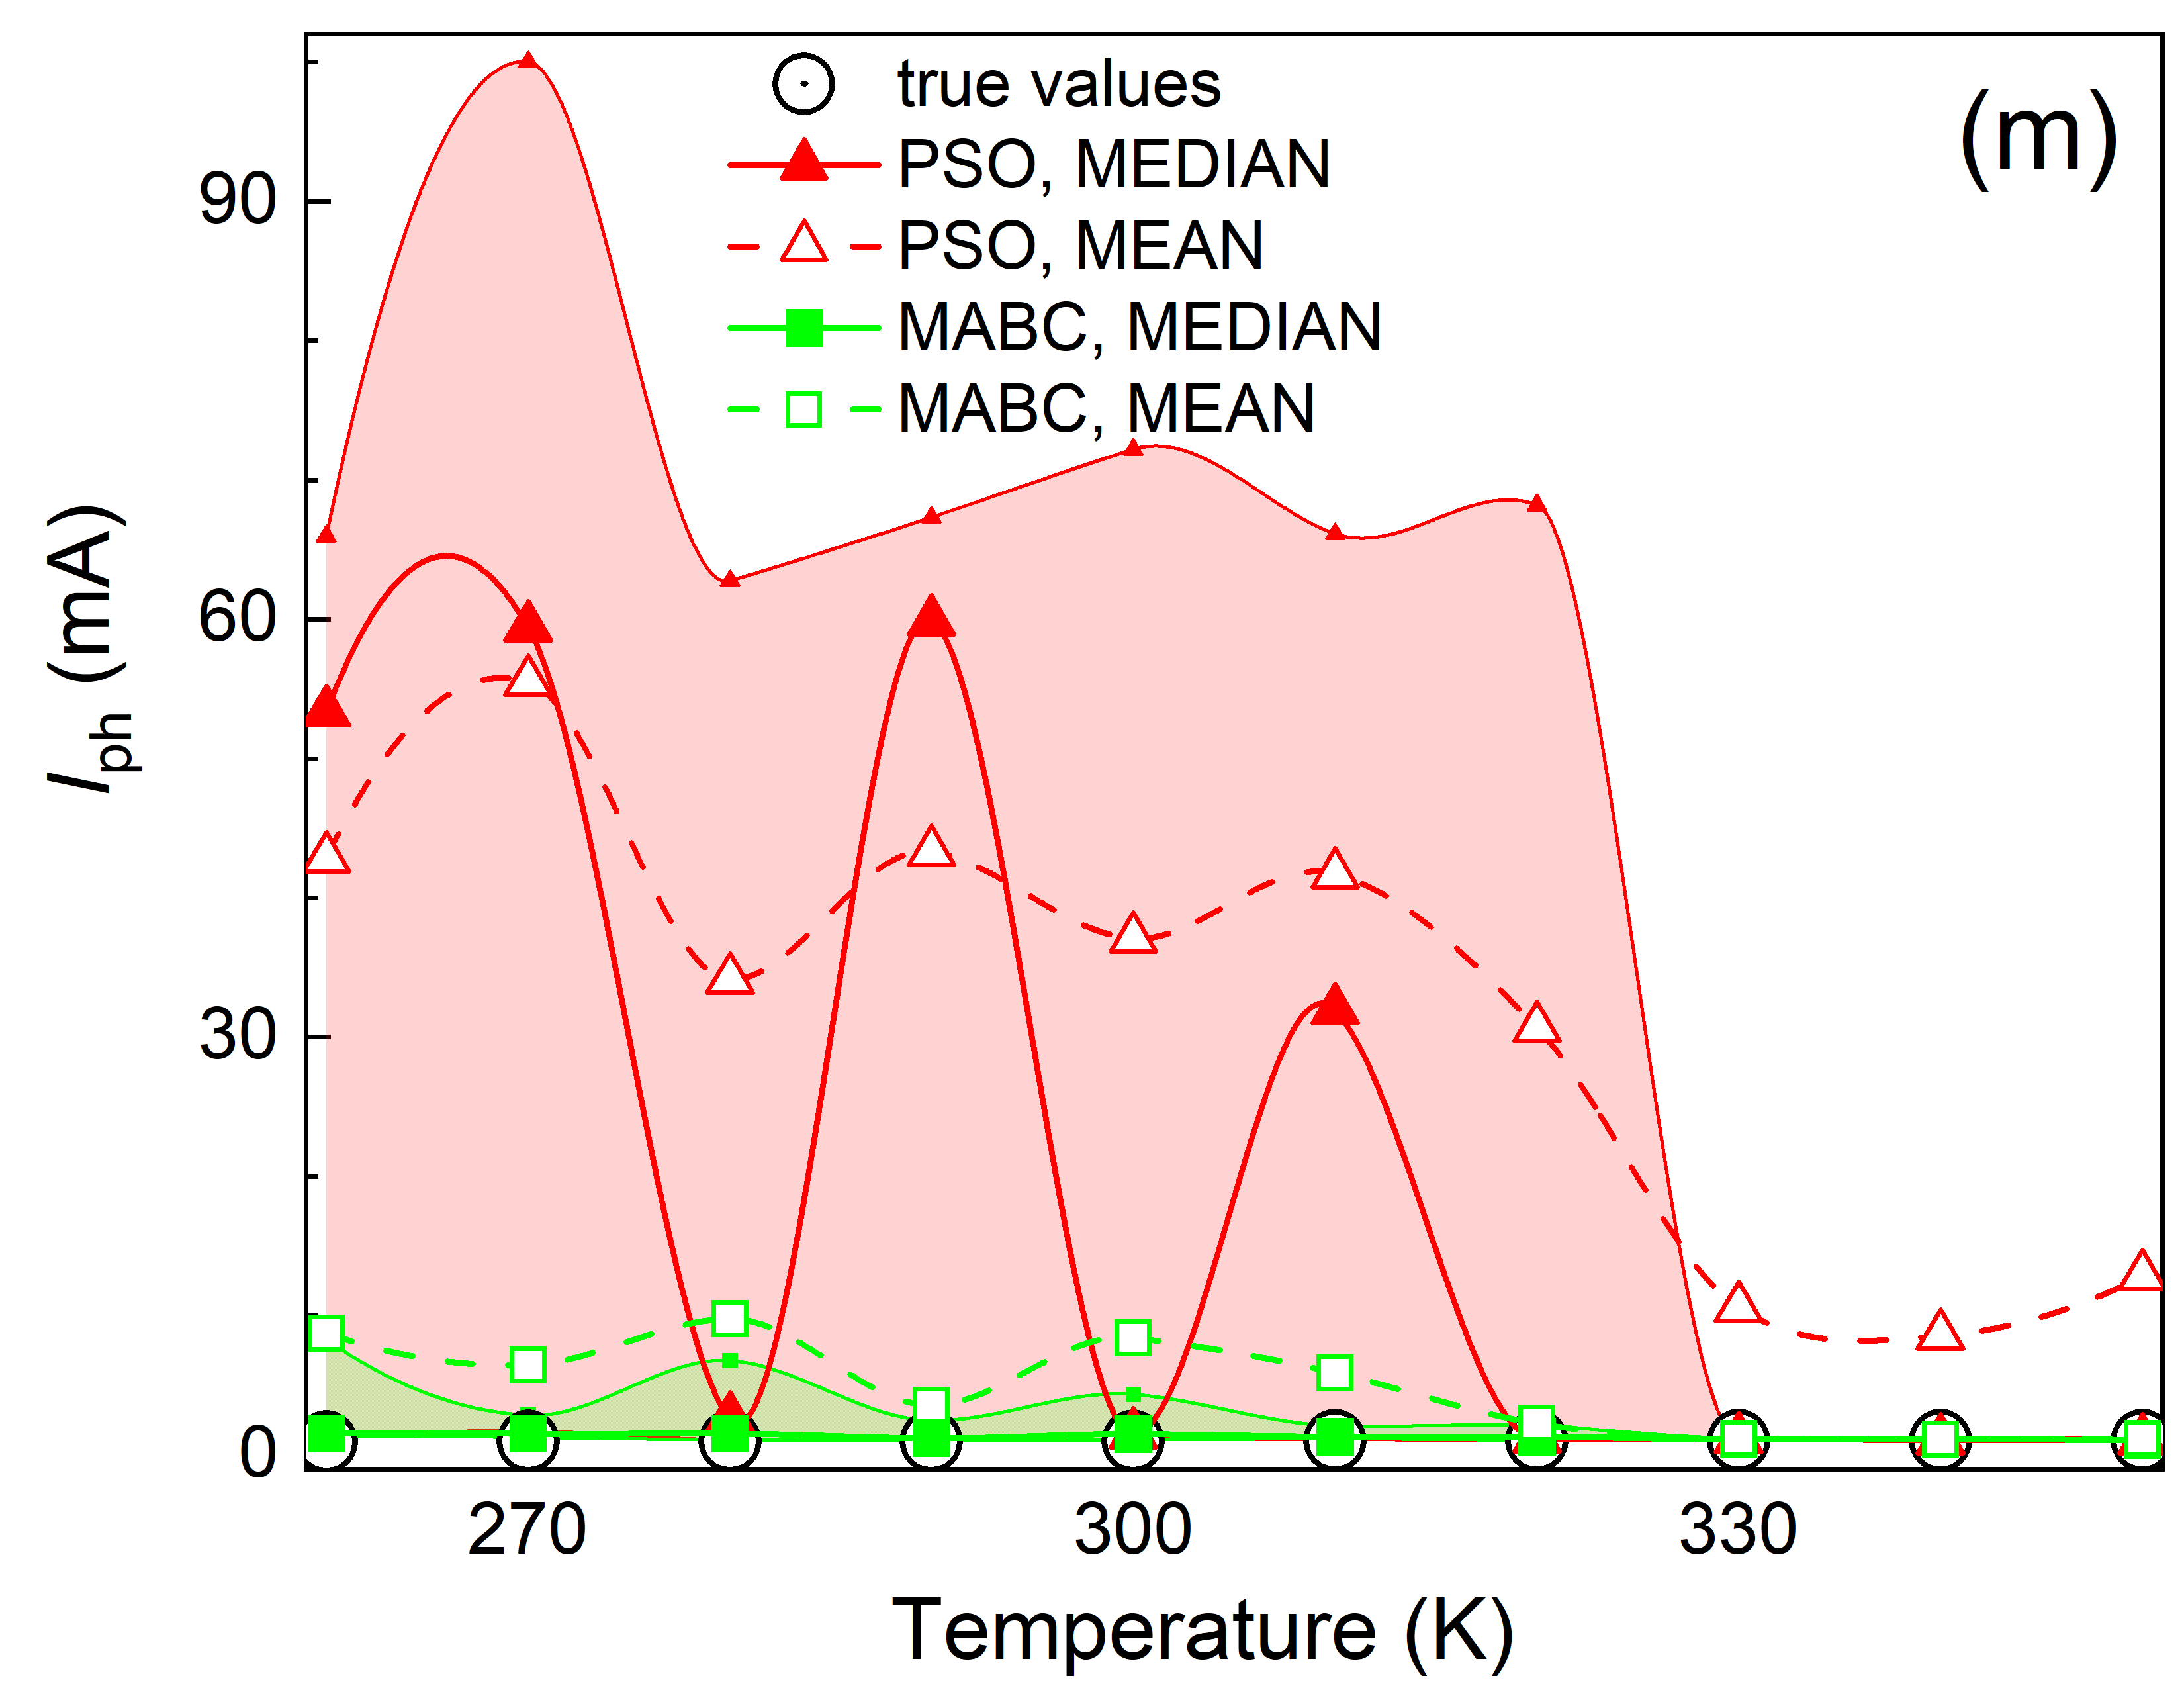
\includegraphics[width=.32\textwidth]{AfigM}
        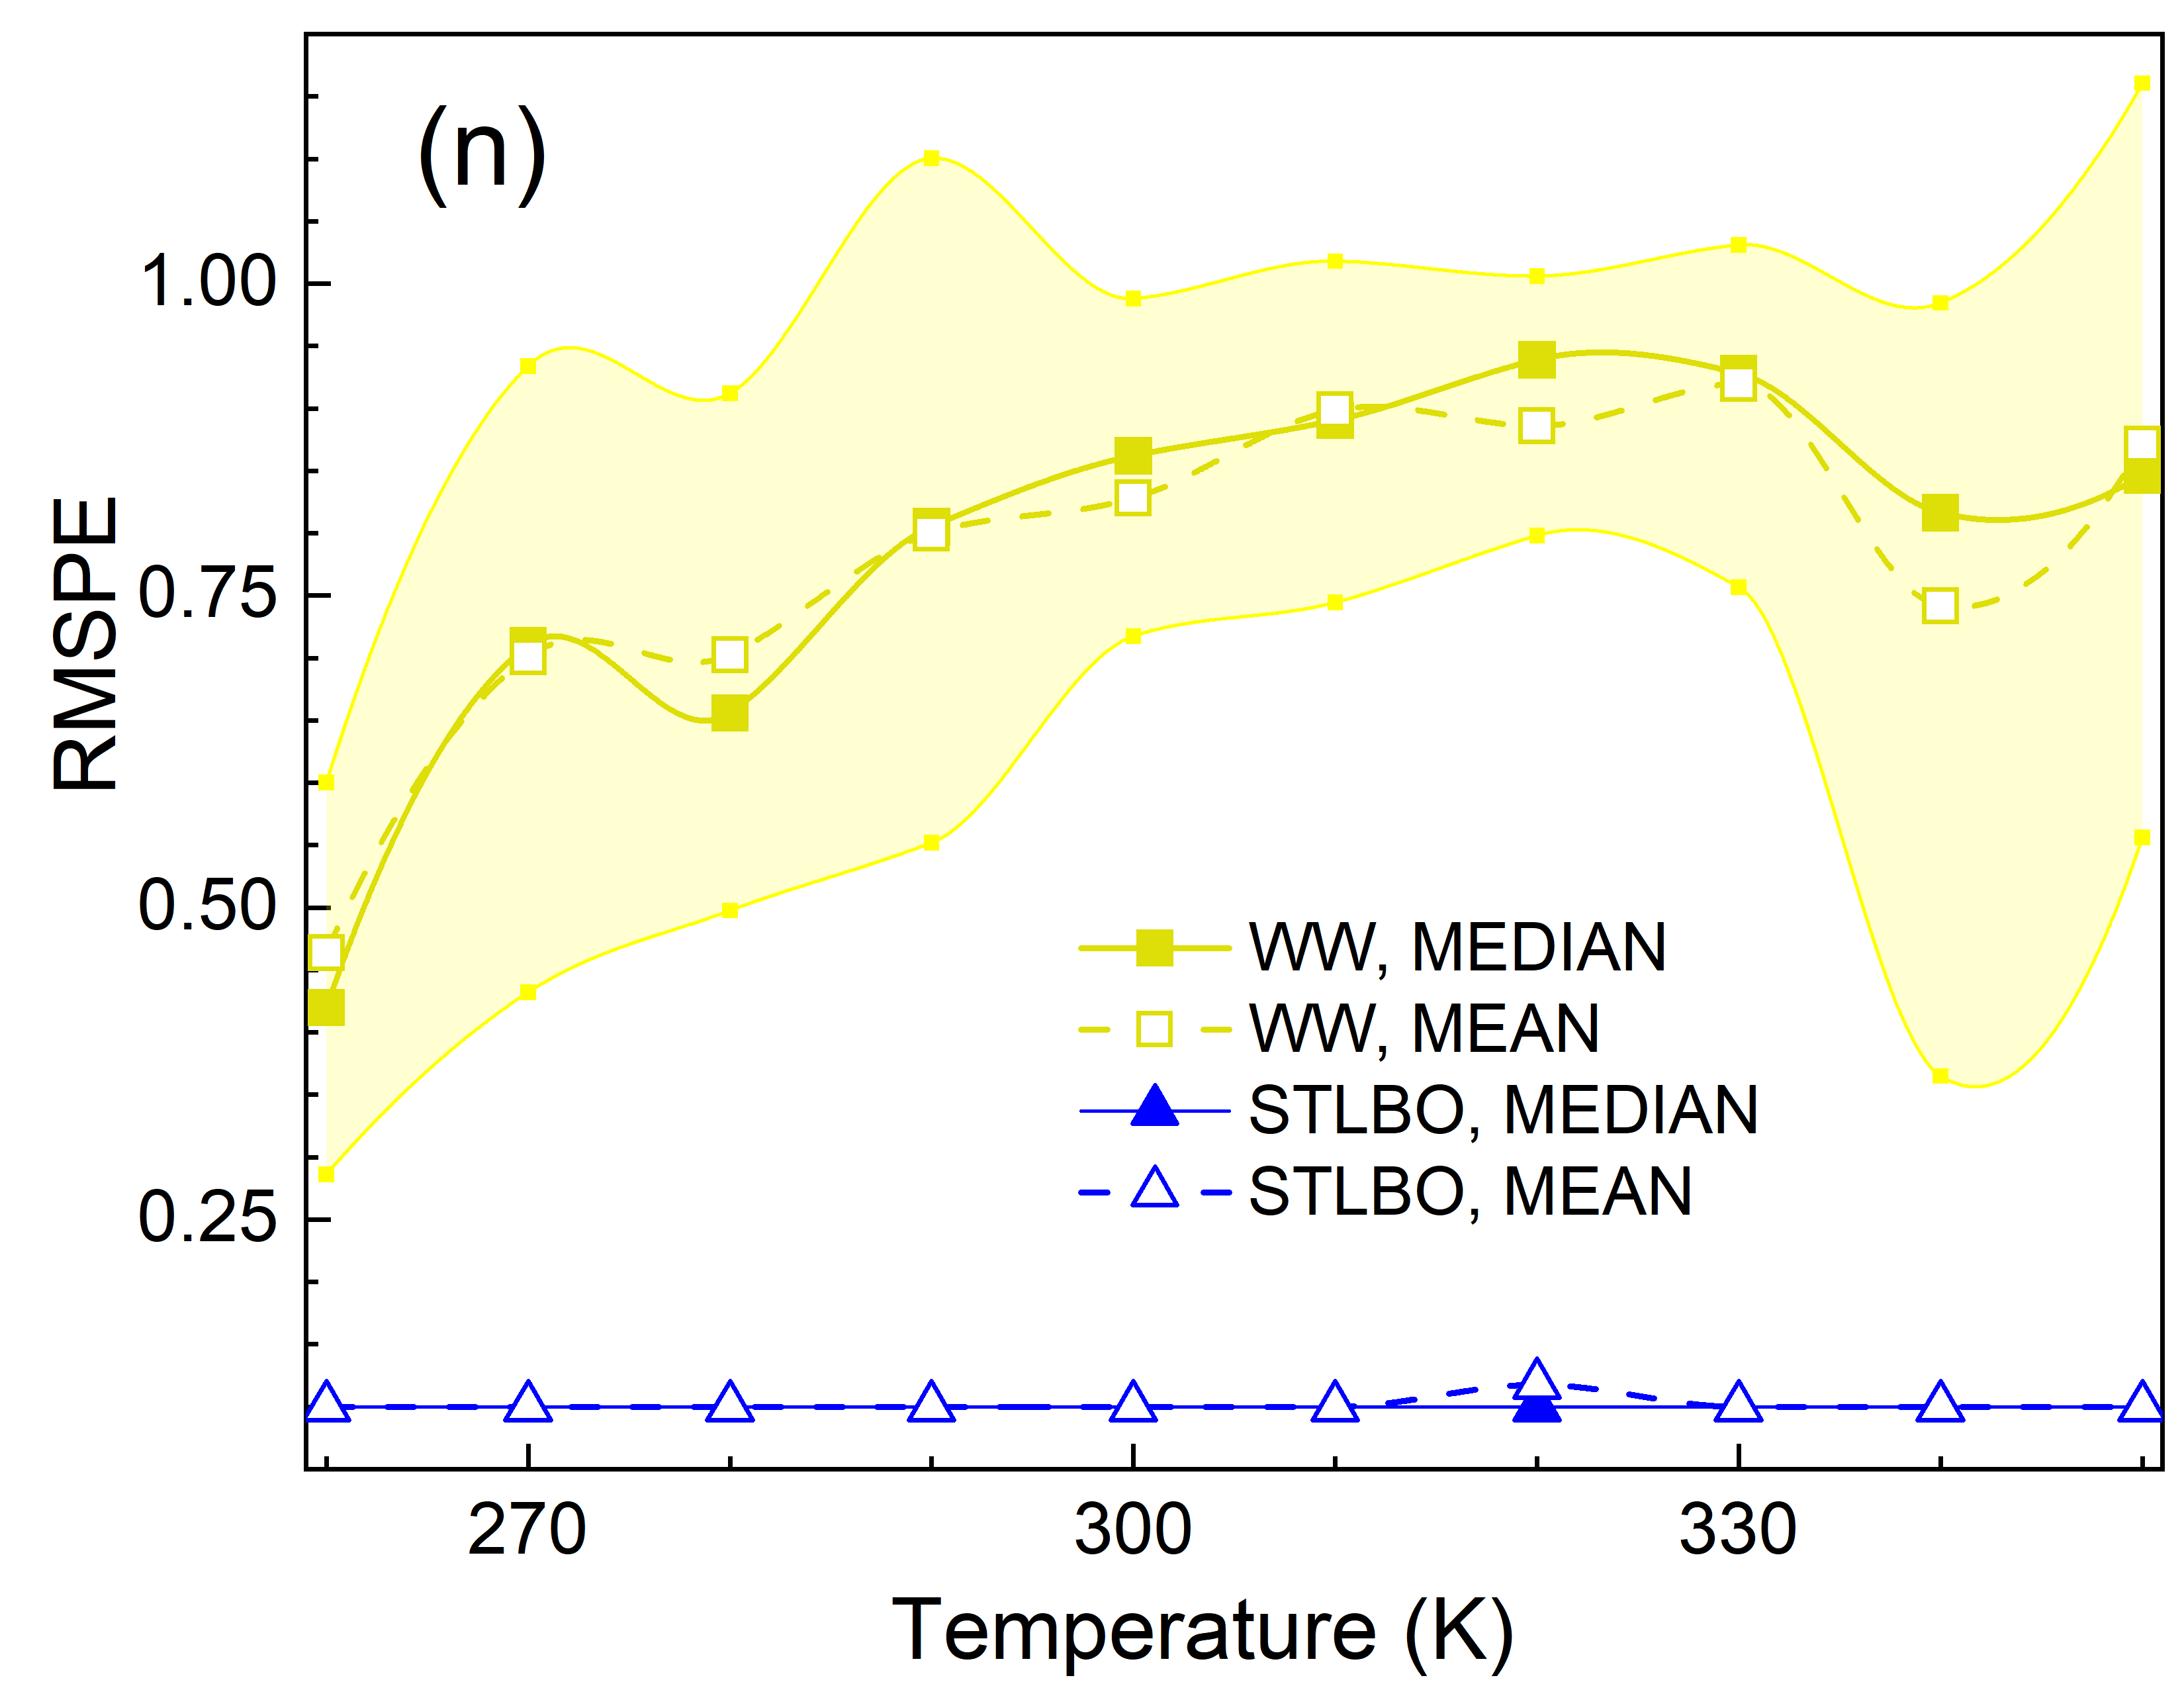
\includegraphics[width=.32\textwidth]{AfigN}
        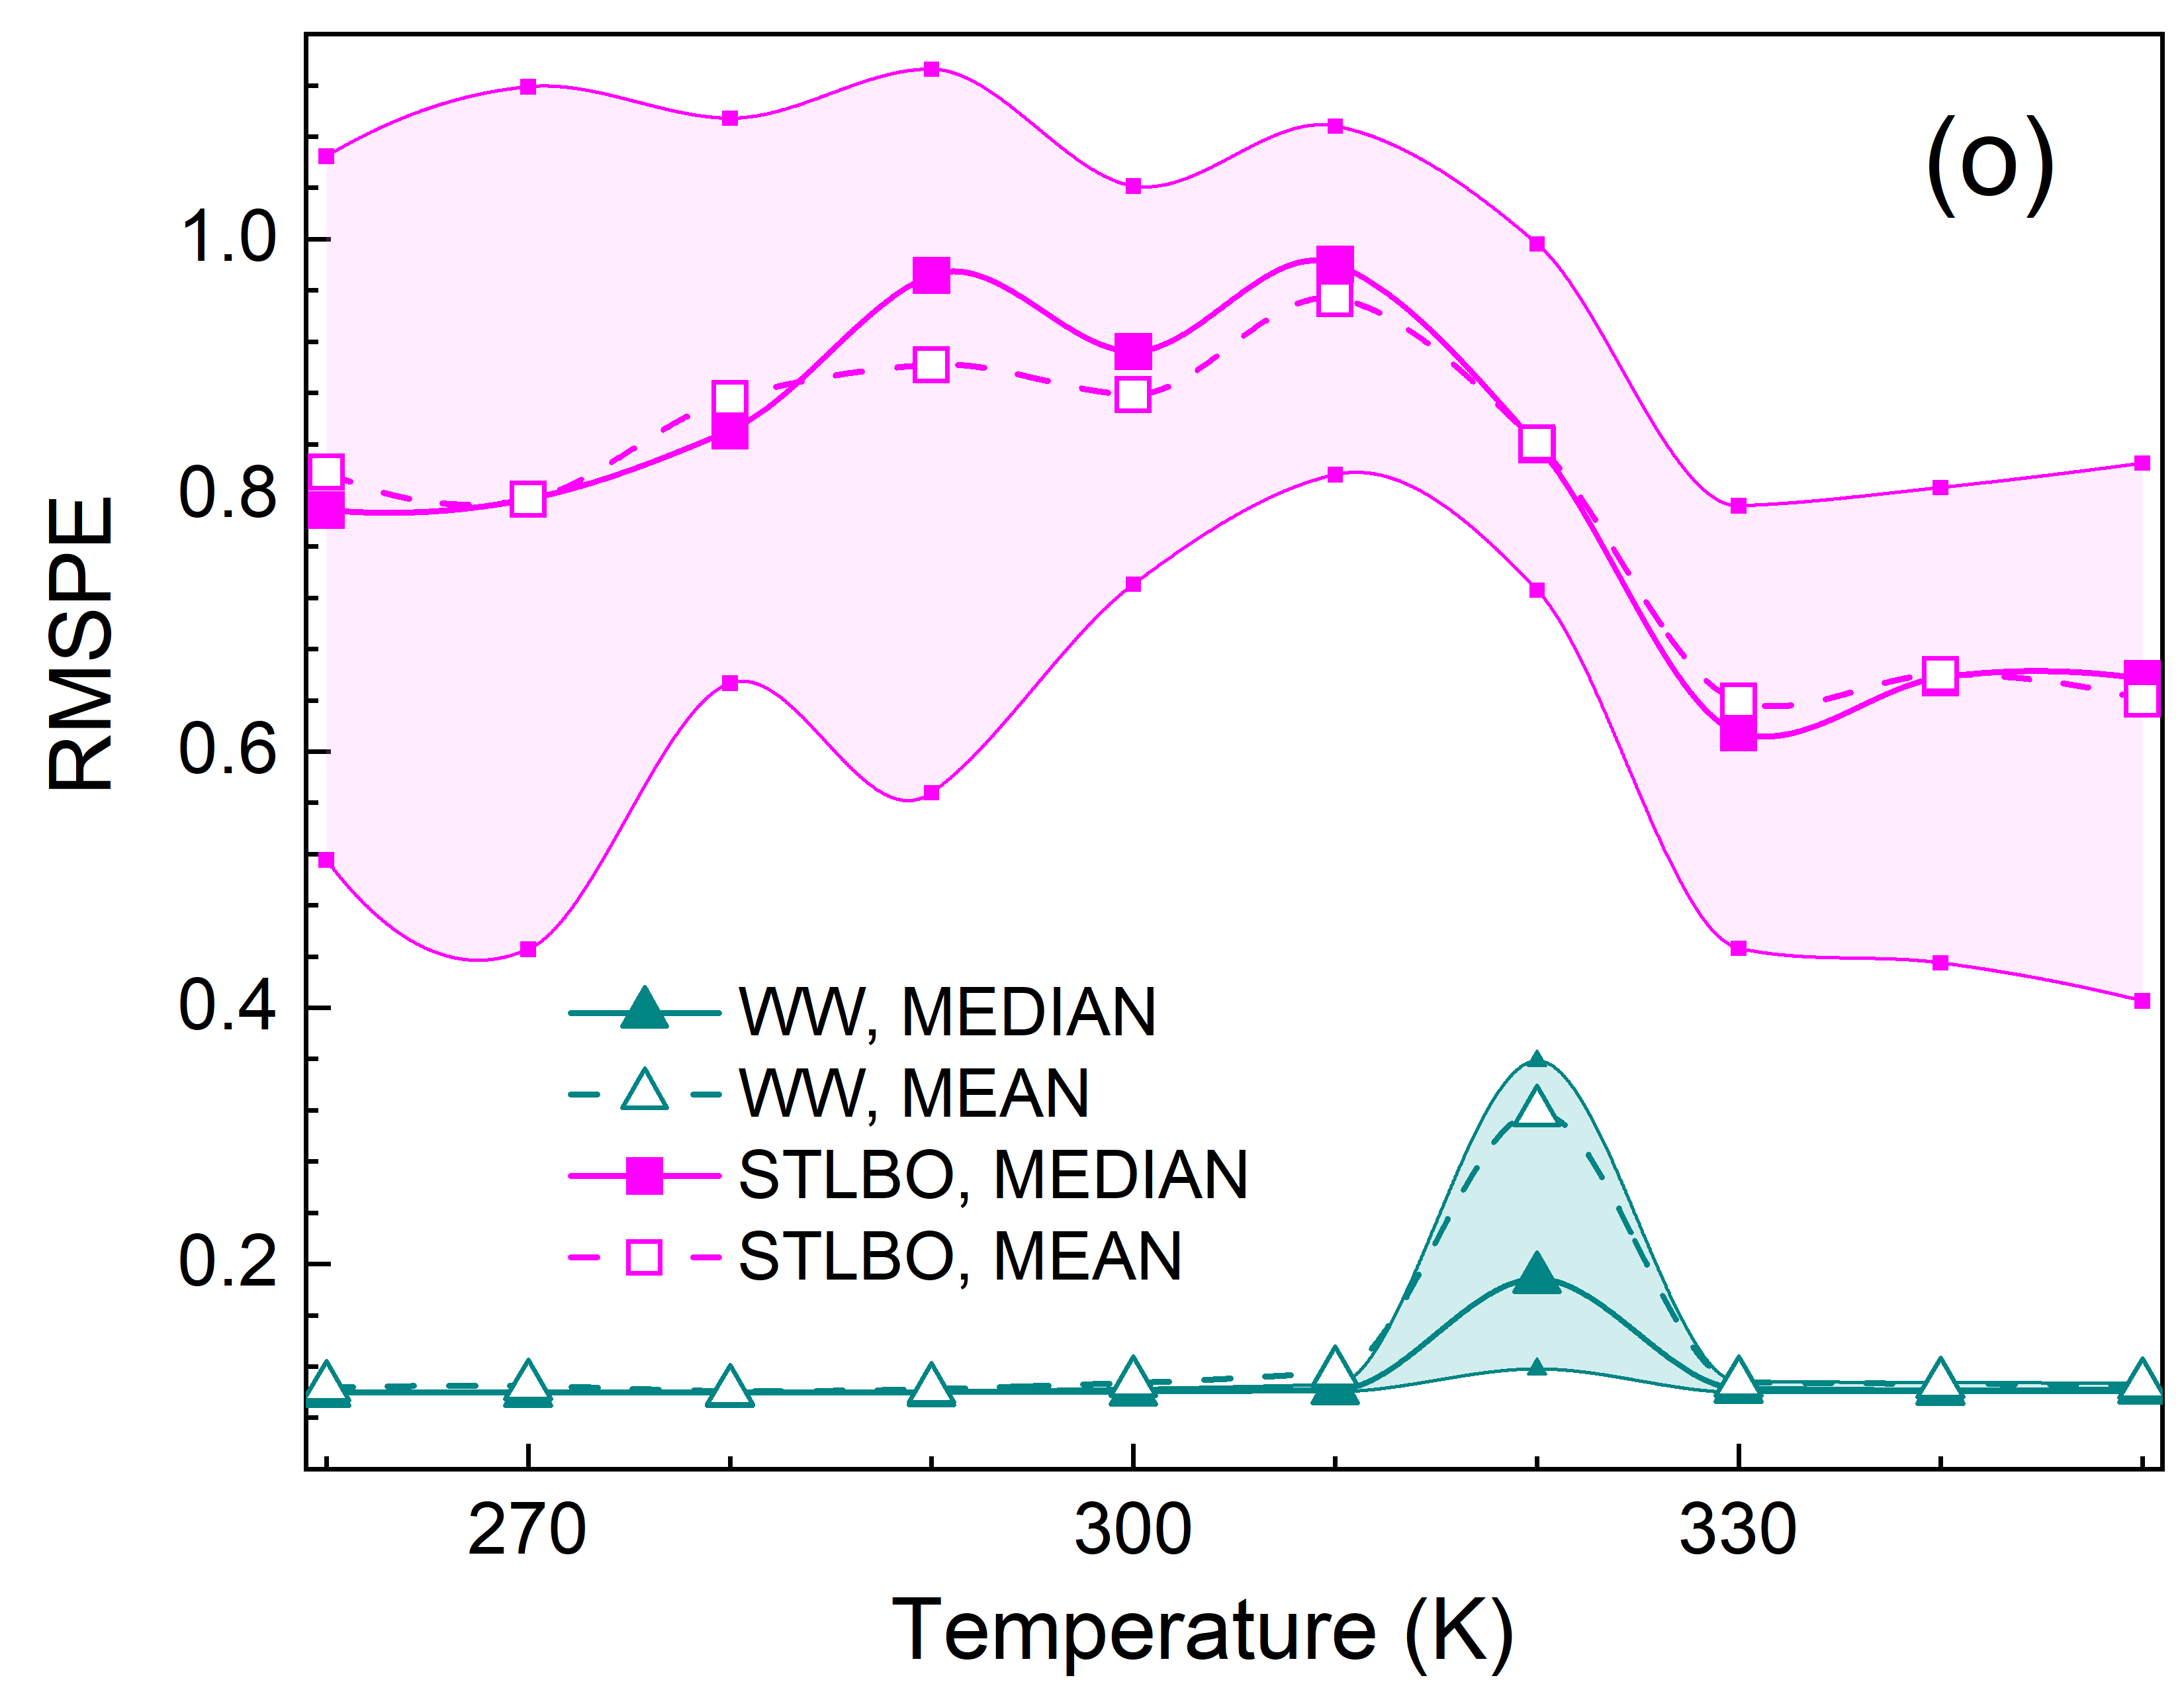
\includegraphics[width=.32\textwidth]{AfigO}
	  \caption{Dependences of the $I_{01}$ (a, b), $n_1$ (c), $R_\mathrm{p1}$ (d), $I_{02}$ (e, f),
               $n_2$ (g, h), $R_\mathrm{p2}$ (i, j), $R_\mathrm{s}$ (k), $I_\mathrm{ph}$ (l, m), and RMSPE (n, o)
               evaluation by different algorithm on the synthesis temperature.
               The IV-set is used.
               The circles represent the values, which have been used in IV curve simulations,
               the filled marks represent the median values, and the empty marks represent the mean values.
               The colored regions correspond to the IQR.
               The lines only serve as guide to the eye.
               }\label{figTDepIVset}
\end{figure*}


In the IV--set case, a comprehensive nonparametric statistical analysis of algorithms efficiency was performed on all parameters collected from all simulated curves.
In this scenario, $n$ had a value of 81:
\begin{equation*}
n= 10\,T\mathrm{values}\times(8\,\mathrm{APE}_\mathrm{MEDIAN}+1\,\mathrm{RMSPE}_\mathrm{MEDIAN})+1\,t_\mathrm{run}\,.
\end{equation*}
%10 temperature values $\times(\mathrm{APE}_\mathrm{MEDIAN}+1\mathrm{RMSPE}_\mathrm{MEDIAN})+1t_\mathrm{run}$.

%subsequent analysis. In order to assess the statistical performance
%of WSO and each other method on the CEC-2017 test suite, the
%mean error values of all methods in all dimensions and the rank
%of each method in each dimension were taken into account. The
%average rankings of WSO in conjunction with other methods




%In these tables, ‘+’ indicated that the null
%hypothesis H0 was rejected and ICO performed better, while ‘−’
%indicated that the null hypothesis H0 was rejected; however, ICO
%performed worse. The ‘=’ indicates a failure to reject the null
%hypothesis, and also there is no statistical difference between the
%two algorithms. The counts of statistical significant cases (+/−/=)
%are presented in the last row of Tables 13–17

\begin{table*}[<options>]
\caption{The results of Wilcoxon signed-rank test with a level of significance $\alpha = 0.05$ in the IV-set case.
         The ``+'' indicated that the null hypothesis was rejected, and the control algorithm (in the row) performed better
         then the comparison algorithm (in the column).
         The ``0'' indicates to rejection of the hypothesis about outperforming the control algorithm.
         }\label{tblWilIVset}
\begin{tabular*}{\tblwidth}{@{}LCCCCCCCCCCCCCCC@{}}
\toprule
Control & \multicolumn{14}{C}{Comparison algorithm}&Total \\
algorithm  &DE&EBLSHADE&ADELI&NDE&MABC&TLBO&GOTLBO&STLBO&PSO&IJAYA&ISCA&NNA&CWOA&WW&$(+/=/-)$\\ % Table header row
\midrule
DE&$\blacksquare$&0&0&0&+&0&+&0&+&0&+&+&+&+&7/0/6\\
EBLSHADE&+&$\blacksquare$&0&+&+&0&+&0&+&+&+&+&+&+&10/0/3\\
ADELI&+&+&$\blacksquare$&+&+&+&+&+&+&+&+&+&+&+&13/0/0\\
NDE&+&0&0&$\blacksquare$&+&0&+&0&+&+&+&+&+&+&9/0/4\\
MABC&0&0&0&0&$\blacksquare$&0&+&0&+&0&+&+&+&+&6/0/7\\
TLBO&+&+&0&+&+&$\blacksquare$&+&0&+&+&+&+&+&+&11/1/1\\
GOTLBO&0&0&0&0&0&0&$\blacksquare$&0&+&0&+&+&+&+&5/0/8\\
STLBO&+&+&0&+&+&0&+&$\blacksquare$&+&+&+&+&+&+&11/1/1\\
PSO&0&0&0&0&0&0&0&0&$\blacksquare$&0&0&0&0&0&0/4/9\\
IJAYA&+&0&0&0&+&0&+&0&+&$\blacksquare$&+&+&+&+&8/0/5\\
ISCA&0&0&0&0&0&0&0&0&0&0&$\blacksquare$&0&0&0&0/3/10\\
NNA&0&0&0&0&0&0&0&0&0&0&0&$\blacksquare$&0&0&0/3/10\\
CWOA&0&0&0&0&0&0&0&0&0&0&0&0&$\blacksquare$&0&0/4/9\\
WW&0&0&0&0&0&0&0&0&0&0&0&+&0&$\blacksquare$&1/3/9\\
\bottomrule
\end{tabular*}
\end{table*}


\begin{figure}[]
	\centering
		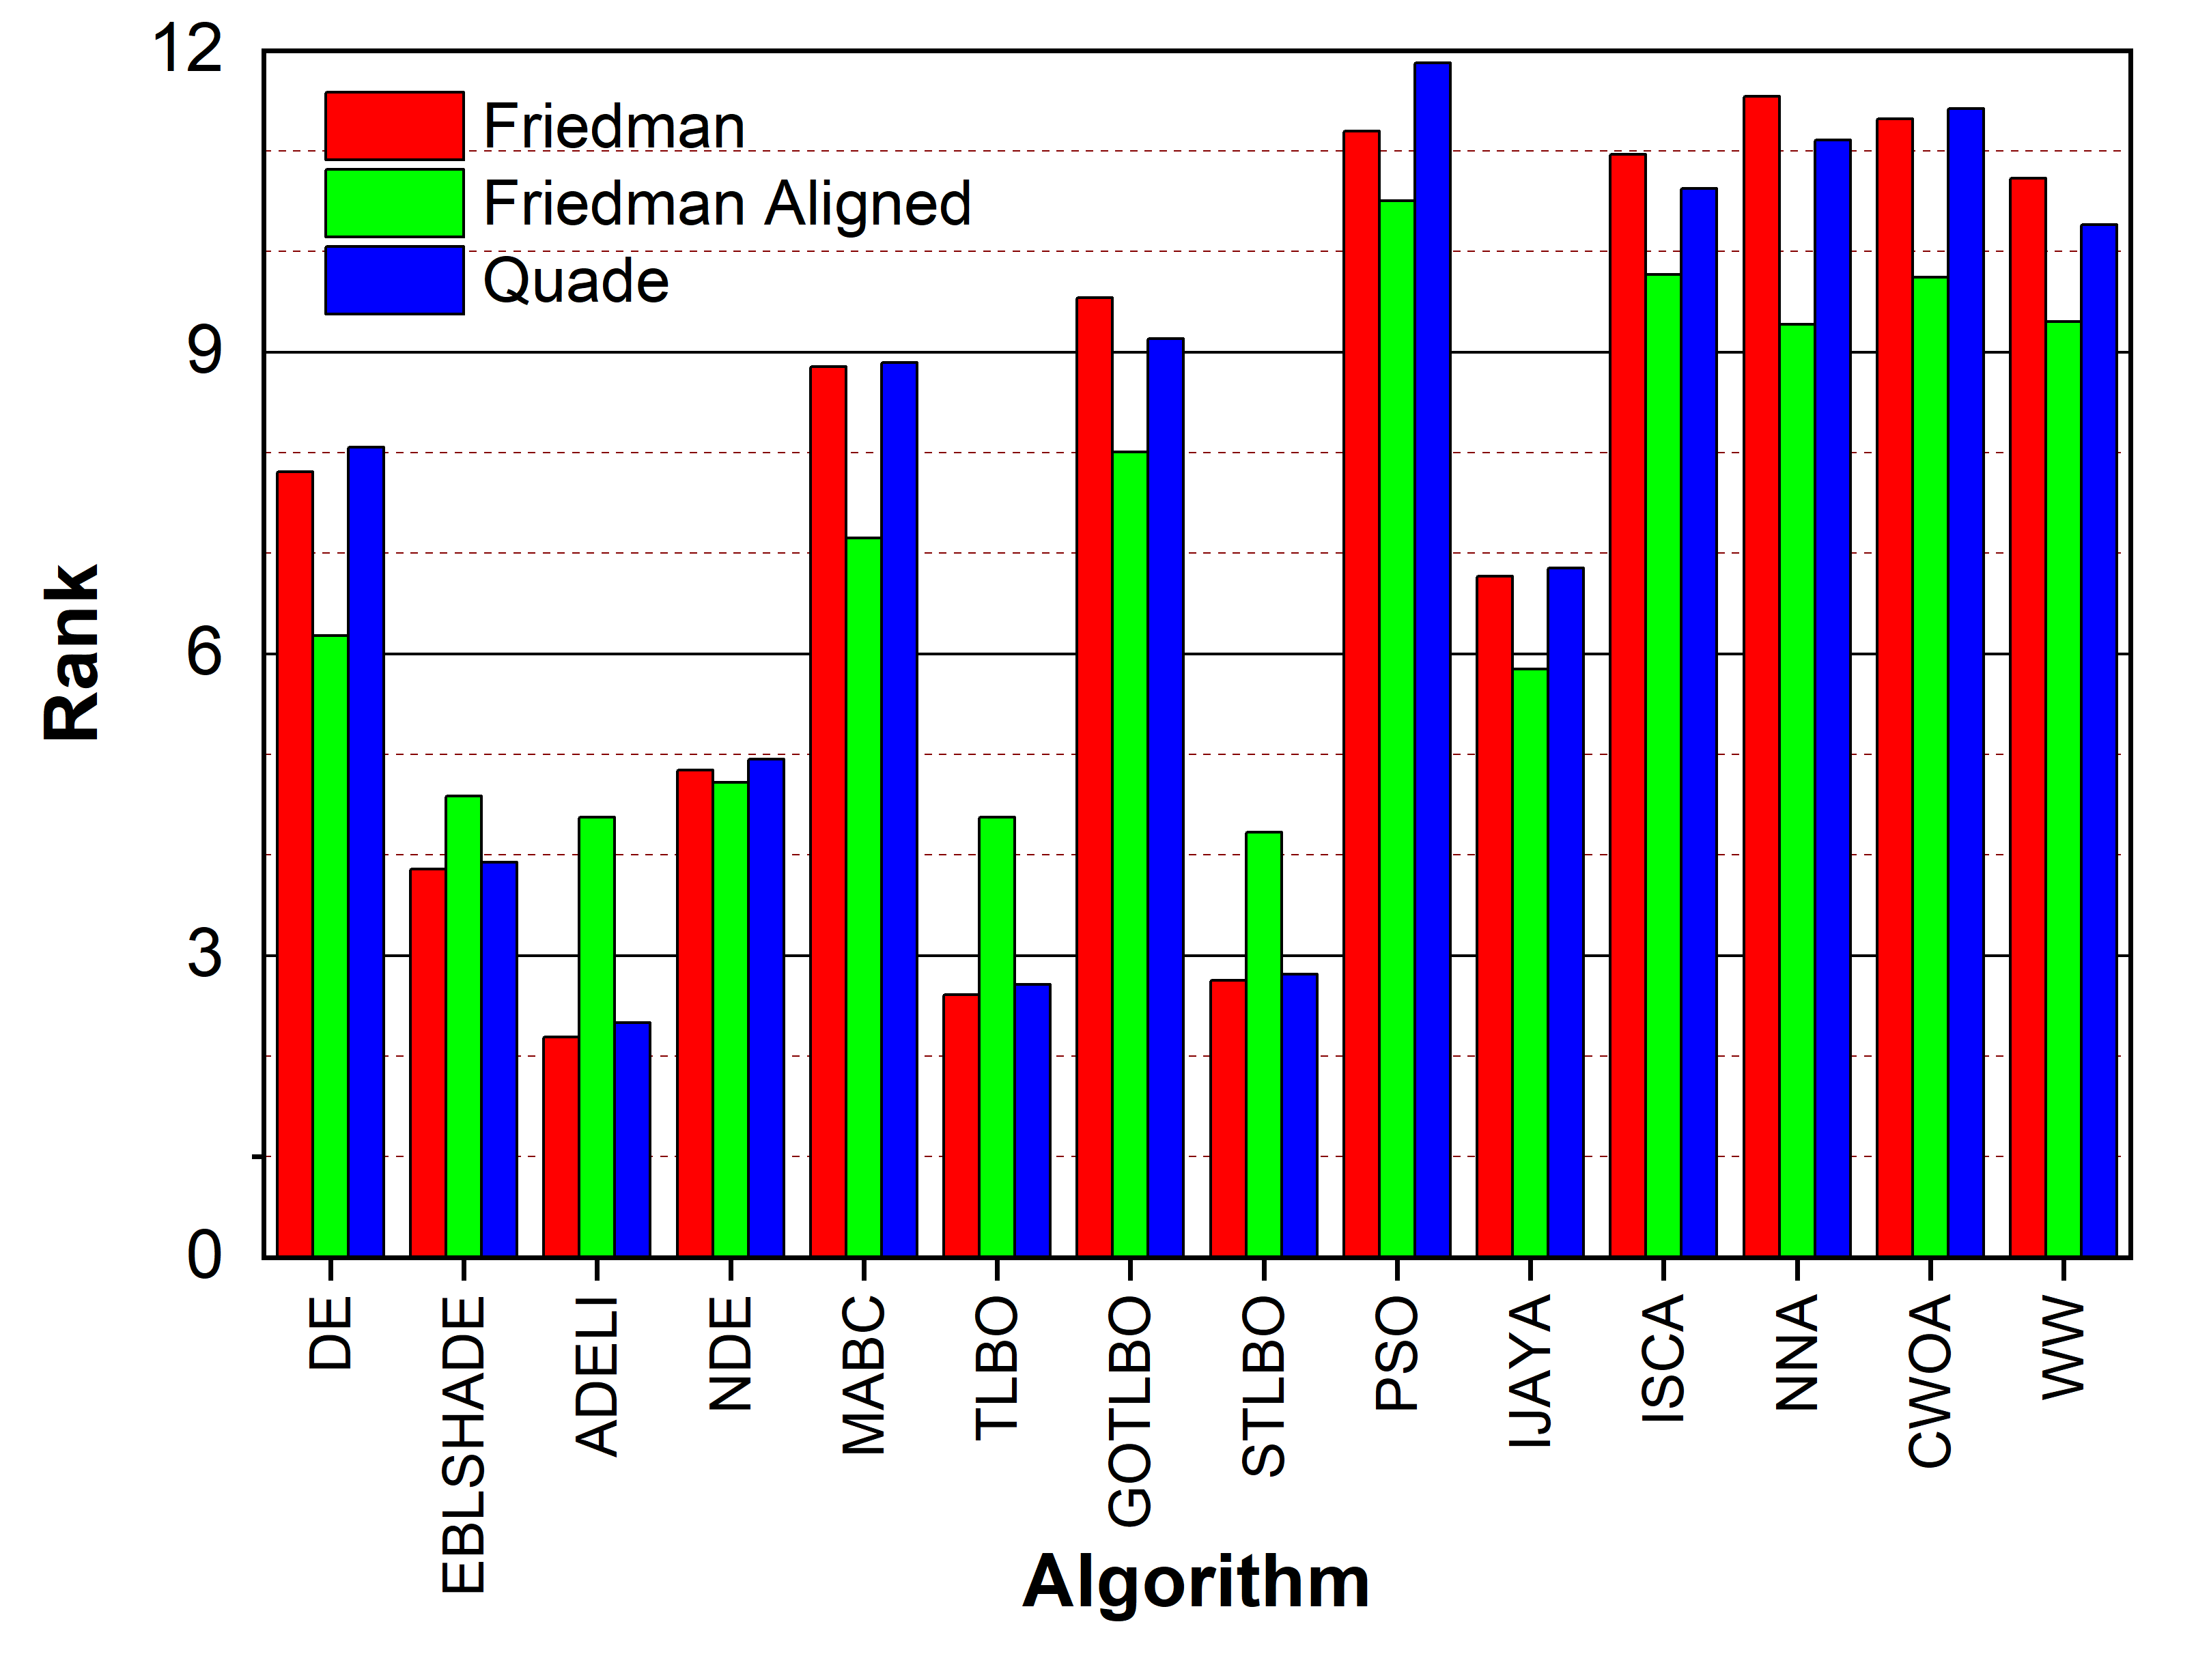
\includegraphics[width=1.0\columnwidth]{FigRankT}
	  \caption{Ranking of the algorithms according to Friedman, Friedman Aligned, and Quade tests in the IV-set case.}\label{figRankIVset}
\end{figure}


\begin{table*}[<options>]
\caption{Adjusted $p$-values for Friedman, Friedman Aligned, and Quade tests in IV--set case.
 STLBO is the control algorithm.}\label{tbl1NSTLBO}
\begin{tabular*}{\tblwidth}{@{}LLCCCC@{}}
\toprule
\multirow{2}{*}{Algorithm}& \multirow{2}{*}{Test}& \multicolumn{4}{C}{post-hoc procedure} \\
  & &Finner & Holm & Hochberg &Holland\\ % Table header row
\midrule
GOTLBO&	Friedman&<1E-13&<1E-13&<1E-13&<1E-13\\
&Friedman Aligned&1.35278E-10&5.09895E-10&5.09895E-10&5.09895E-10\\
&Quade&1.11445E-03&4.11614E-03&4.11614E-03&4.10873E-03\\
PSO&Friedman&<1E-13&<1E-13&<1E-13&<1E-13\\
&Friedman Aligned&<1E-13&<1E-13&<1E-13&<1E-13\\
&Quade&8.22938E-06&8.22941E-06&8.22941E-06&8.22938E-06\\
NNA&Friedman&<1E-13&<1E-13&<1E-13&<1E-13\\
&Friedman Aligned&<1E-13&<1E-13&<1E-13&<1E-13\\
&Quade&2.21284E-05&5.61727E-05&5.61727E-05&5.61713E-05\\
CWOA&Friedman&<1E-13&<1E-13&<1E-13&<1E-13\\
&Friedman Aligned&<1E-13&<1E-13&<1E-13&<1E-13\\
&Quade&1.48311E-05&2.73807E-05&2.73807E-05&2.73803E-05\\
DE&Friedman&2.32081E-13&8.03357E-13&8.03357E-13&8.03357E-13\\
&Friedman Aligned&1.74950E-09&6.45968E-09&6.45968E-09&6.45968E-09\\
&Quade&6.44257E-03&2.38175E-02&2.38175E-02&2.35824E-02\\
IJAYA&Friedman&2.17645E-10&8.03613E-10&8.03613E-10&8.03613E-10\\
&Friedman Aligned&3.63299E-09&1.25757E-08&1.25757E-08&1.25757E-08\\
&Quade&3.78757E-02&1.31885E-01&1.31885E-01&1.25109E-01\\
MABC&Friedman&1.75608E-09&6.61909E-09&6.61909E-09&6.61909E-09\\
&Friedman Aligned&<1E-13&<1E-13&<1E-13&<1E-13\\
&Quade&1.54776E-03&5.83595E-03&5.83595E-03&5.82137E-03\\
WW&Friedman&7.44635E-09&2.74942E-08&2.74942E-08&2.74942E-08\\
&Friedman Aligned&<1E-13&<1E-13&<1E-13&<1E-13\\
&Quade&1.10078E-04&3.81053E-04&3.81053E-04&3.80989E-04\\
ISCA&Friedman&1.32325E-08&4.58048E-08&4.58048E-08&4.58048E-08\\
&Friedman Aligned&<1E-13&<1E-13&<1E-13&<1E-13\\
&Quade&5.64886E-05&1.73815E-04&1.73815E-04&1.73801E-04\\
NDE&Friedman&9.57698E-04&2.94709E-03&2.94709E-03&2.94383E-03\\
&Friedman Aligned&2.69373E-03&8.29097E-03&8.29097E-03&8.26522E-03\\
&Quade&2.98714E-01&9.55486E-01&9.55486E-01&6.64392E-01\\
EBLSHADE&Friedman&8.62842E-02&2.20533E-01&2.20533E-01&2.04719E-01\\
&Friedman Aligned&3.10807E-02&7.90881E-02&7.90881E-02&7.70214E-02\\
&Quade&5.99120E-01&1.0&1.0&9.01765E-01\\
ADELI&Friedman&1.0&1.0&1.0&1.0\\
&Friedman Aligned&3.64522E-01&6.83937E-01&3.45600E-01&5.66995E-01\\
&Quade&1.0&1.0&1.0&1.0\\
TLBO&Friedman&1.0&1.0&1.0&1.0\\
&Friedman Aligned&3.64522E-01&6.83937E-01&3.45600E-01&5.66995E-01\\
&Quade&1.0&1.0&1.0&1.0\\
\bottomrule
\end{tabular*}
\end{table*}




\begin{figure}[]
	\centering
		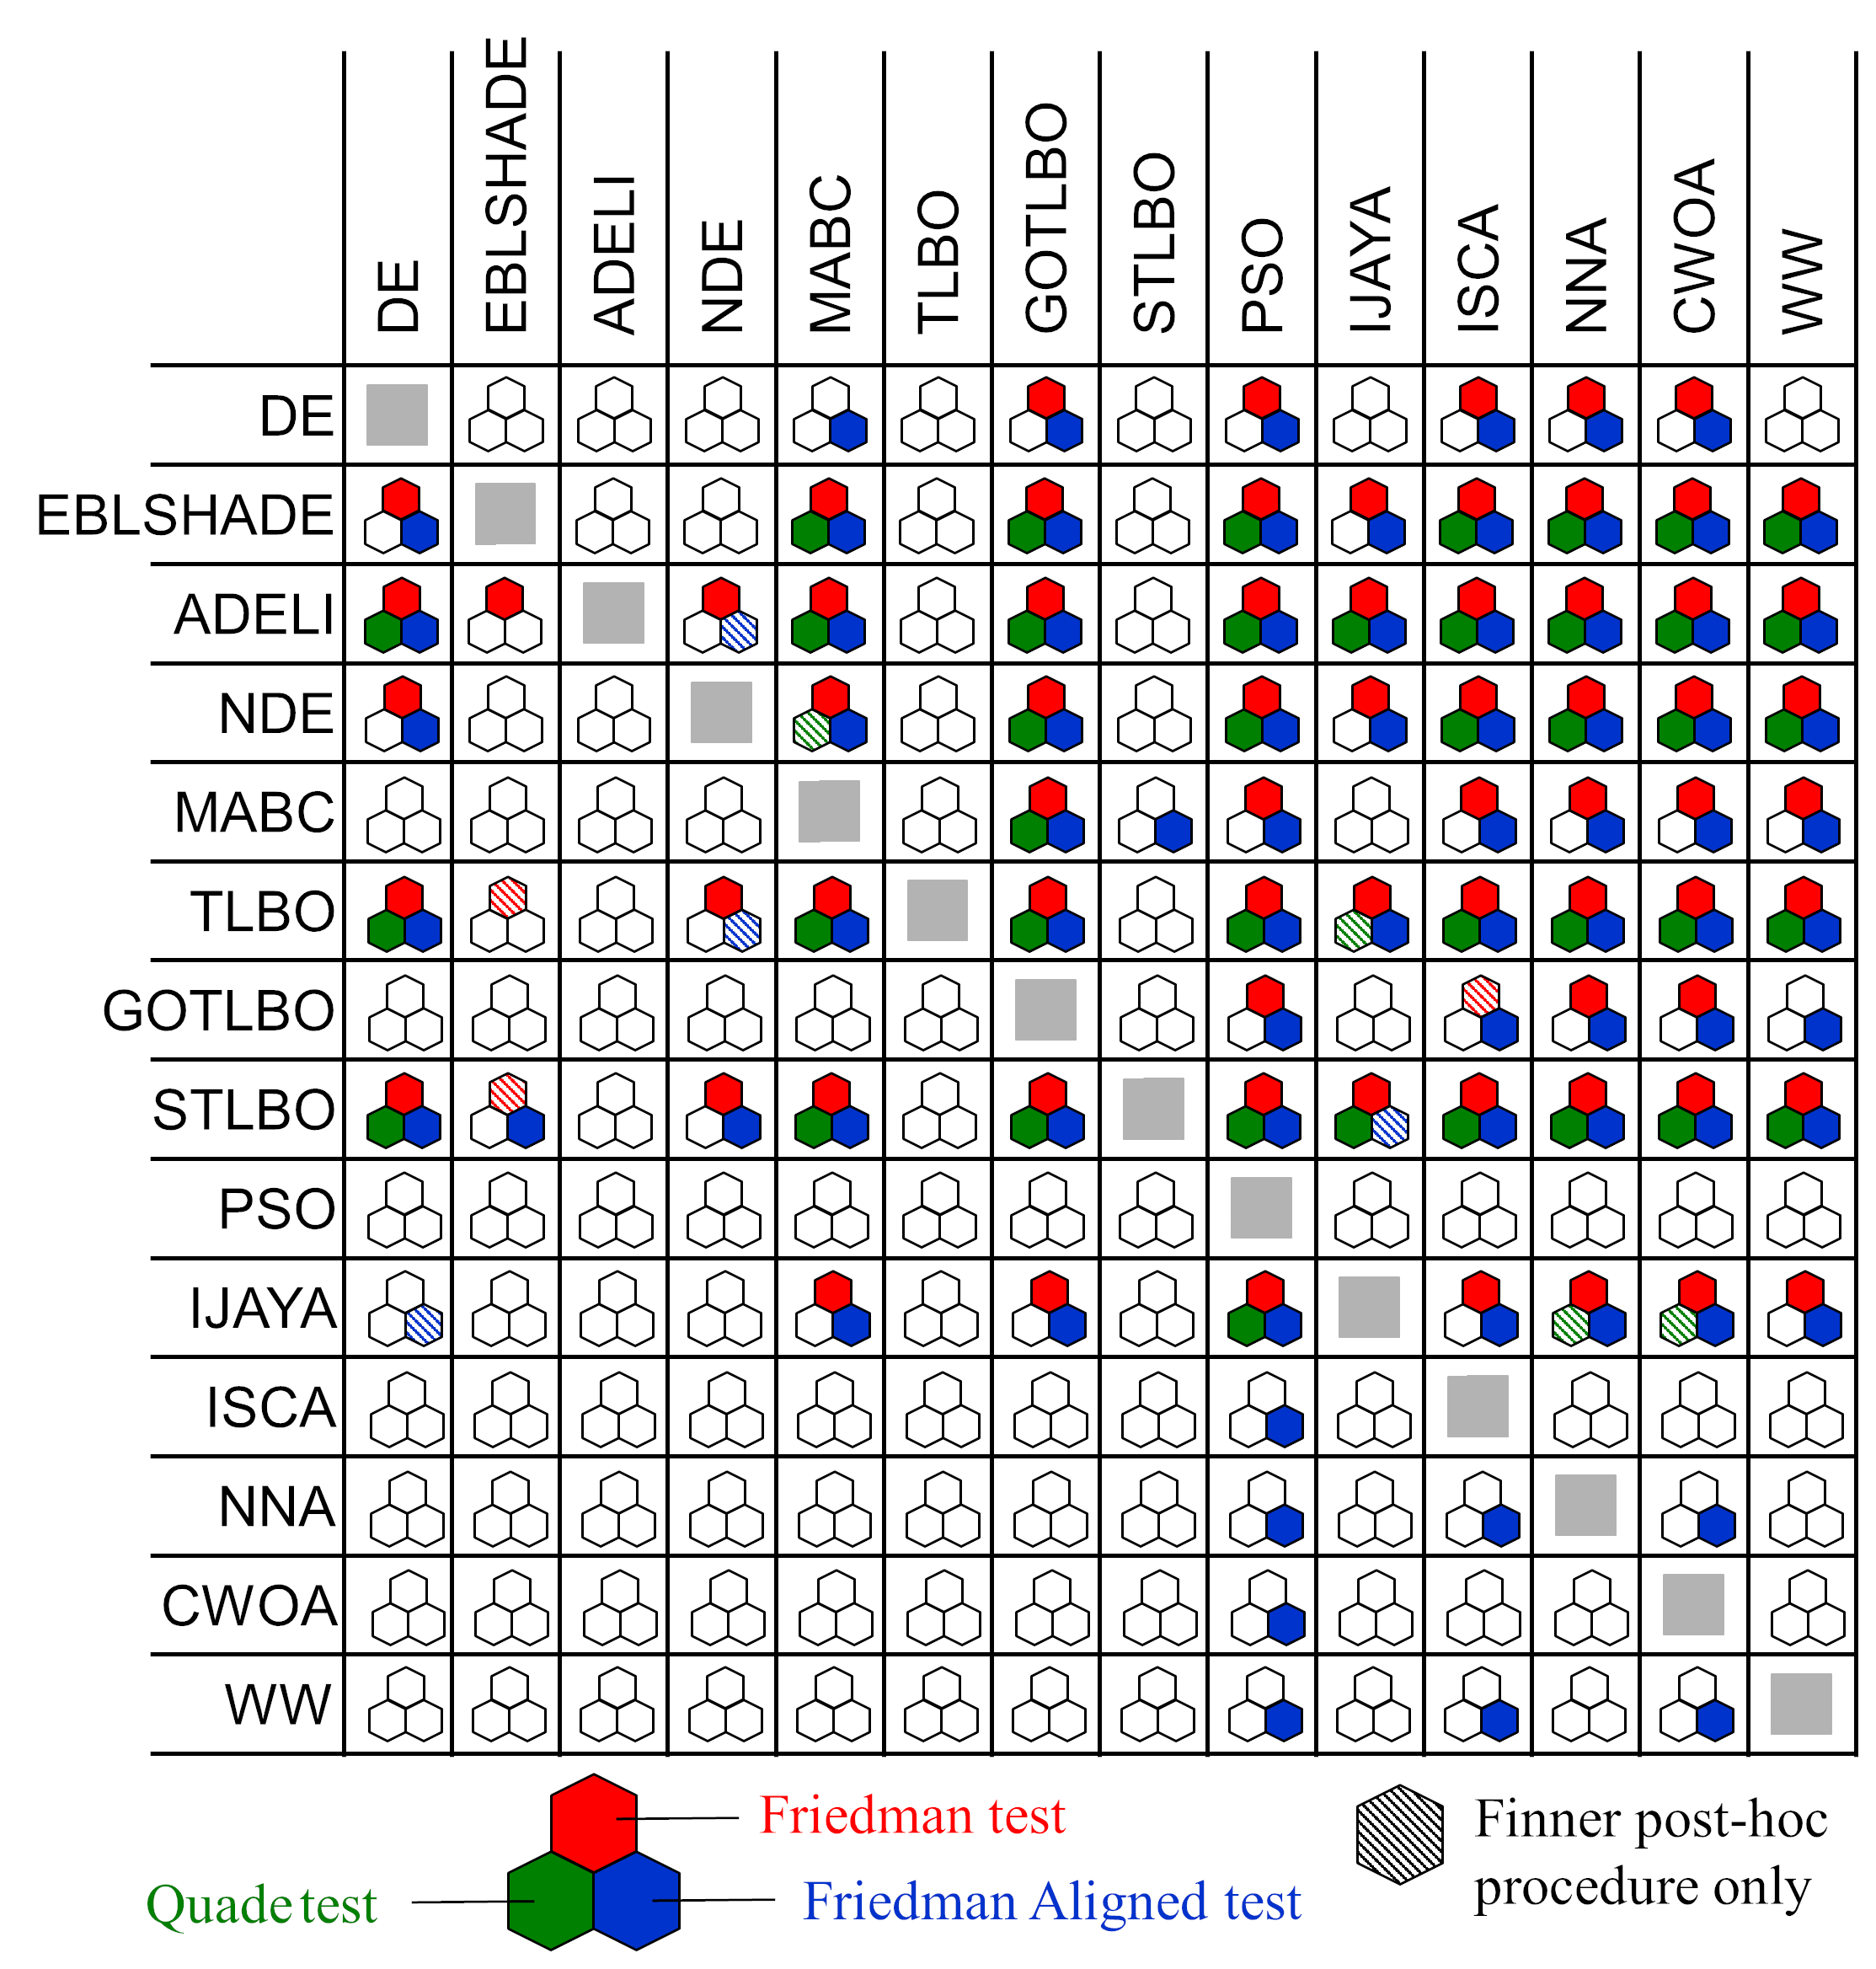
\includegraphics[width=1.0\columnwidth]{N1Tresult}
	  \caption{The results of algorithm $1\times N$ comparison by Friedman, Friedman Aligned, and Quade tests in the IV-set case.
               The colored hexagon indicates that the adjusted $p$-value,
               which tests the hypothesis that an algorithm in a row outperforms the algorithm in a column,
               is not greater than $p_{lim}=0.1$.
               The solid fill signifies that every post-hoc procedure resulted in $p<p_{lim}$;
               the dashed fill indicates that the Finner post-hoc procedure was the only method that produced this result.
               The correspondence between the color and position of the hexagon to a test
               is shown in a legend at the bottom of the figure.
               }\label{figN1RezIVset}
\end{figure}


\begin{table*}[<options>]
\caption{Adjusted $p$-values for tests for multiple $N\times N$ comparisons among all methods
         in the IV--set case ($p<p_{lim}$ are only shown).}\label{tblNNpValue}
\begin{tabular*}{\tblwidth}{@{}LCCC@{}}
\toprule
\multirow{2}{*}{Hypothesis}& \multicolumn{3}{C}{post-hoc procedure} \\
  &Nemenyi & Holm & Shaffer\\ % Table header row
\midrule
EBLSHADE versus WW,
ADELI versus MABC,&&&\\
ADELI versus PSO,
ADELI versus ISCA,&&&\\
ADELI versus NNA,
ADELI versus CWOA,&&&\\
ADELI versus WW,
NDE versus NNA,&&&\\
TLBO versus GOTLBO,
TLBO versus PSO,&&&\\
TLBO versus ISCA,
TLBO versus NNA,&&&\\
TLBO versus CWOA,
STLBO versus GOTLBO, &&&\\
STLBO versus PSO,
STLBO versus NNA, &&&\\
STLBO versus CWOA&<1E-13&<1E-13&<1E-13\\
IJAYA versus NNA&1.61648E-12&1.31450E-12&1.19016E-12\\
EBLSHADE versus MABC&3.75833E-12&3.01492E-12&2.76712E-12\\
NDE versus GOTLBO&4.20286E-12&3.32534E-12&3.09441E-12\\
STLBO versus DE&8.12284E-12&6.33760E-12&5.98055E-12\\
IJAYA versus CWOA&2.31157E-11&1.75273E-11&1.70193E-11\\
TLBO versus DE&4.02505E-11&3.00773E-11&2.96350E-11\\
IJAYA versus PSO&9.52918E-11&7.01599E-11&7.01599E-11\\
IJAYA versus ISCA&1.29115E-09&9.36436E-10&9.36436E-10\\
ADELI versus DE&2.22329E-09&1.56363E-09&1.41704E-09\\
EBLSHADE versus GOTLBO&3.53238E-09&2.44550E-09&2.25141E-09\\
NDE versus MABC&9.68759E-09&6.49388E-09&6.17451E-09\\
IJAYA versus WW&1.72440E-08&1.13697E-08&1.09907E-08\\
NDE versus WW&1.75252E-08&1.13697E-08&1.11699E-08\\
EBLSHADE versus DE&1.82602E-08&1.16384E-08&1.16384E-08\\
EBLSHADE versus ISCA&1.88327E-08&1.17963E-08&1.16384E-08\\
EBLSHADE versus PSO&4.78066E-08&2.94194E-08&2.94194E-08\\
ADELI versus GOTLBO&4.98663E-08&3.01390E-08&3.01390E-08\\
EBLSHADE versus CWOA&7.52618E-08&4.46609E-08&4.21797E-08\\
STLBO versus MABC&8.60481E-08&5.01159E-08&4.82248E-08\\
NDE versus ISCA&9.60138E-08&5.48650E-08&5.38099E-08\\
DE versus NNA&1.60867E-07&9.01562E-08&9.01562E-08\\
EBLSHADE versus NNA&1.68788E-07&9.27404E-08&9.01562E-08\\
TLBO versus MABC&2.16163E-07&1.16396E-07&1.14020E-07\\
NDE versus PSO&4.07575E-07&2.14985E-07&2.14985E-07\\
STLBO versus WW&4.16995E-07&2.15371E-07&2.15371E-07\\
TLBO versus WW&6.32636E-07&3.19794E-07&3.19794E-07\\
NDE versus CWOA&8.17751E-07&4.04382E-07&4.04382E-07\\
STLBO versus ISCA&8.33647E-07&4.04382E-07&4.04382E-07\\
DE versus CWOA&1.47836E-06&6.98567E-07&6.98567E-07\\
DE versus PSO&4.48549E-06&2.07023E-06&2.07023E-06\\
DE versus ISCA&3.33823E-05&1.50404E-05&1.46735E-05\\
NDE versus DE&1.56228E-04&6.86718E-05&6.86718E-05\\
DE versus WW&2.41908E-04&1.03675E-04&1.03675E-04\\
IJAYA versus GOTLBO&7.27786E-04&2.95913E-04&2.95913E-04\\
MABC versus NNA&1.28945E-03&5.10114E-04&5.10114E-04\\
ADELI versus NDE&1.70688E-03&6.56493E-04&6.56493E-04\\
MABC versus CWOA&6.56486E-03&2.45281E-03&2.45281E-03\\
MABC versus PSO&1.46075E-02&5.29723E-03&5.13671E-03\\
TLBO versus NDE&2.83112E-02&9.95560E-03&9.95560E-03\\
MABC versus ISCA&6.08528E-02&2.07301E-02&2.07301E-02\\
STLBO versus NDE&6.70463E-02&2.21032E-02&2.21032E-02\\
IJAYA versus MABC&6.92376E-02&2.21032E-02&2.21032E-02\\
GOTLBO versus NNA&1.07776E-01&3.31618E-02&3.31618E-02\\
MABC versus WW&2.35963E-01&6.74180E-02&6.74180E-02\\
\bottomrule
\end{tabular*}
\end{table*}



\begin{figure}[]
	\centering
		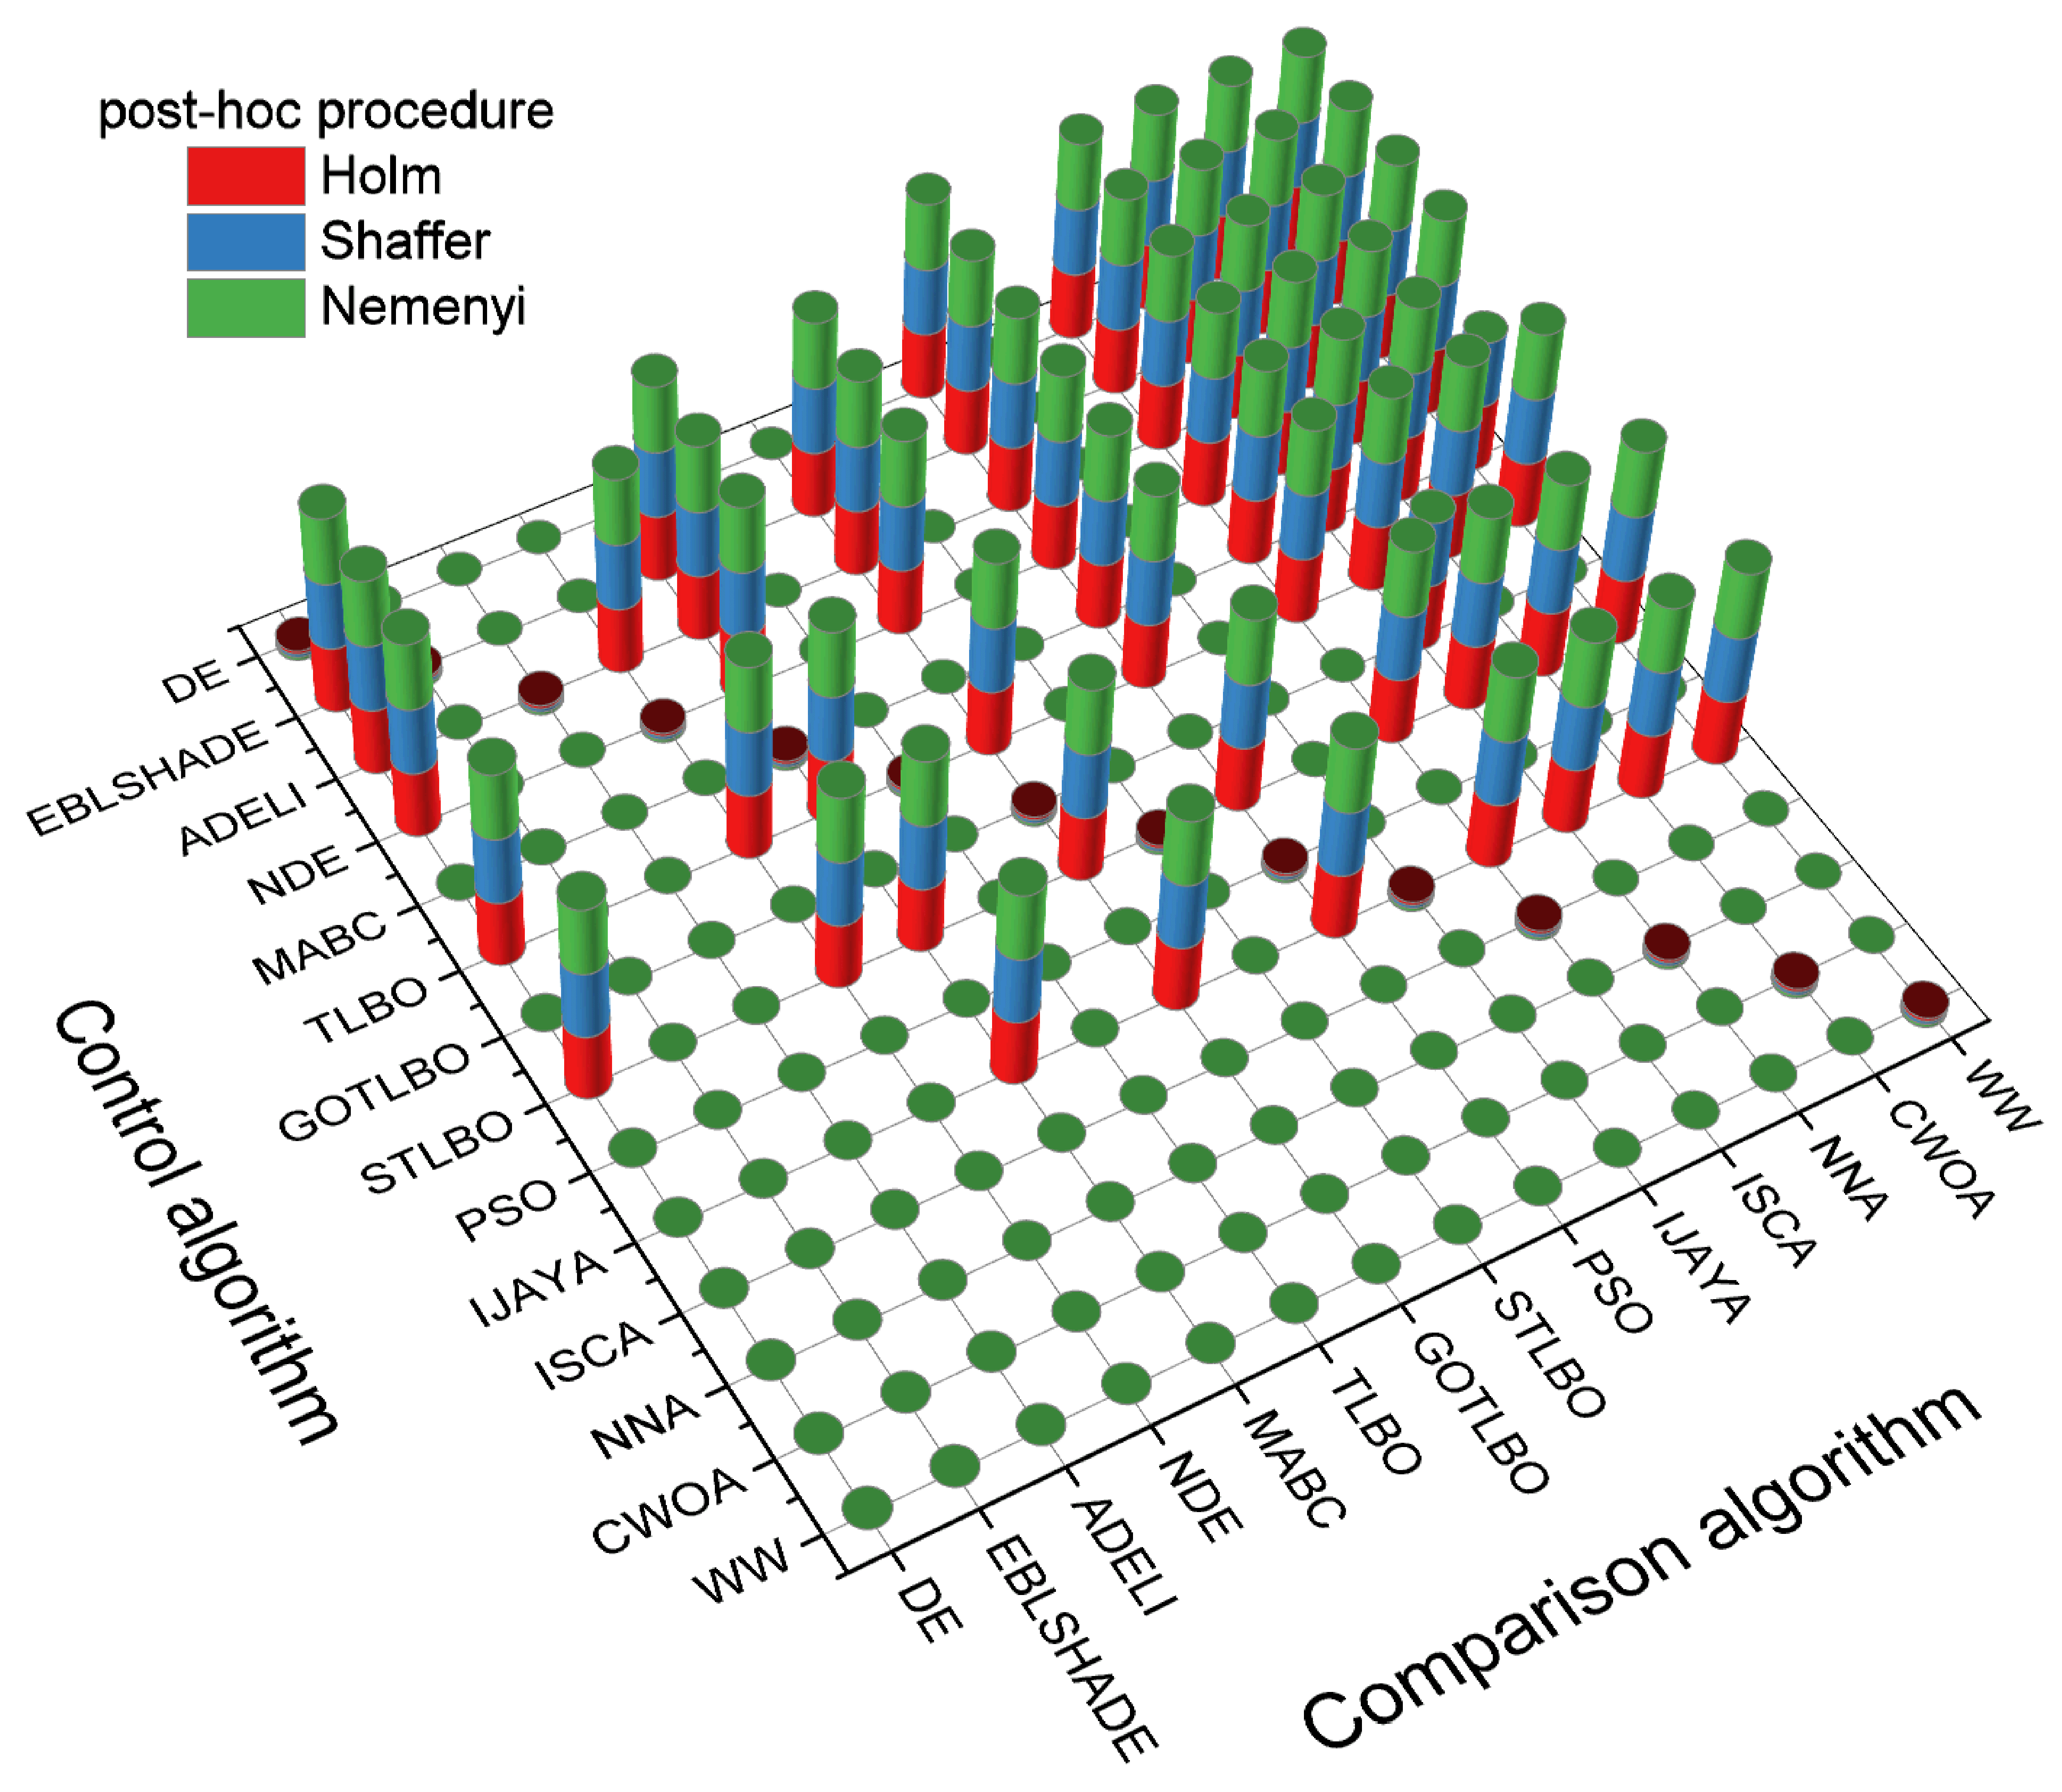
\includegraphics[width=1.0\columnwidth]{NNresult}
	  \caption{The results of multiple comparisons among all algorithms in the IV-set case.
               The colored cylinder indicates that the adjusted p-value,
               which tests the control algorithm outperforms the comparison algorithm,
               is not greater than $p_{lim}=0.1$.
               The correspondence between the color of the cylinder to a post-hoc procedure is shown in the figure's legend.
               }\label{figNNRezIVset}
\end{figure}


\section{Conclusion}

%Box Plot of some functions from F1–F10 for all algorithms using CEC2017 and Dim = 30

%KnowBasSys_233_107555
%Fig. 5. The statistical results produced by Wilcoxon sign-rank test on 45 test functions. ‘‘Win’’ denotes EJAYA beat the compared algorithm; ‘‘Lose’’ indicates EJAYA
%is inferior to the compared algorithms; ‘‘Tie’’ denotes EJAYA has the same performance with the compared algorithms
%стовпчикова діаграма з кількостями перемог, поразк, нічий
%Table 6
%The results between EJAYA and the compared algorithms (GWO, WOA, SCA and JAYA) produced by Wilcoxon sign-rank test with a significant level α = 0.05 on 45
%test functions.

%3.5. Computational time analysis
%Another evaluation criterion used to compare the algorithms’
%performance is to compare their execution time in terms of
%solving different problems. The mean sum of 30 different runs
%in each algorithm is shown in Fig. 10 to solve 39 functions
%(unimodal, multimodal, fixed dimension multimodal, composite
%functions and CEC2019 functions). According to the figure, execution time of ICO is less than execution time of known and
%efficient algorithms like DE, LASHADE-SPACMA, LSHADE-cnEpSin
%and HGSO.
%To evaluate the usability of the GOA relative to other algorithms, we conduct time tests on all three dimensions.



%In order to statistically verify the excellent results obtained by GOA, we use the nonparametric Wilcoxon Ranksum test to determine whether the GOA algorithm is significantly different from other comparison algorithms. The
%significance level alpha is taken as 0.05, the p-values of the tests are given in Tables 5–7, and the data with p-values
%greater than 0.05 have been shown in bold.

%In this subsection, we show and analyze the statistical results
%of SO and other seven state-of-art algorithms using 30 CEC 2017
%functions. Table 4 shows the results of SO and other comparative algorithms in terms of mean (average), best (min), worst
%(max), median, and standard deviation (STD). from this table, it
%can be seen that SO outperform other mentioned metaheuristic
%algorithms. It is notable that SO has the best average results in 22
%functions from 29 ones and the second-best in 3 other functions
%whereas it ranked third in other 2 functions. GOA has ranked first
%in only 3 functions however, each of MFO, and HHO has achieved
%the best average in only 2 functions. On the other hand, SO has
%ranked first in 11 functions in standard deviation (STD) and has
%the second-best STD values in other 8 functions. Also, LSHADEEpSin has recorded the second-best algorithm in terms of STD
%values as it ranked first in 7 functions. Each of L-SHADE, HHO,
%and TEO has ranked first twice.


%For all the algorithms, a population size and maximum iteration
%equal to 30 and 500 have been utilized. The number of search
%agents n and number of iteration T are commonly set based on trial
%and error basis and should be proportional to the size of the search
%space and the complexity of the fitness function. In this work, we
%adopted the same setting for n and T as in the original paper by
%in Mirjalili

%перекласти на англійську "Переважна більшість використаних алгоритмів показують гарні результати при оцінці параметрів сонячних елементів в межах звичних моделей "

%покращити стилістику, виправити граматичні та стилістичні помилки, використовуючи стиль наукової статті "The method is based on DE by incorporating an adaptive local search scheme with Lagrange interpolation to enhance the exploitation capability to accelerate the convergence speed."


%3.2.6. Wilcoxon signed-rank test
%In order to show the obtained results of ICO that is significantly different from the other randomized algorithms, the
%Wilcoxon Signed-Rank Test was used for pairwise comparison.
%The test was performed by using the global minimum values
%obtained by performing 30 runs for problem based pairwise comparison of the algorithms. The significance value α was chosen to
%be 0.05 with null hypothesis H0; that is, there is no difference
%between the median of the solutions obtained after the same
%test problem is executed by algorithms A and B, i.e. median (A)
%= median(B). Also, to determine whether algorithm A yielded
%statistically the better solution than algorithm B or whether alternative hypothesis was valid, the sizes of the ranks provided
%by the Wilcoxon Signed-Rank test (T+ and T−) were thoroughly
%examined.
%-------------------------------------------------------------
%The non-parametric statistical results of the ICO algorithm
%versus other algorithms based on the Wilcoxon Signed-Rank Test
%with the statistical significance level α = 0.05 are also summarized in Tables 13–17. In these tables, ‘+’ indicated that the null
%hypothesis H0 was rejected and ICO performed better, while ‘−’
%indicated that the null hypothesis H0 was rejected; however, ICO
%performed worse. The ‘=’ indicates a failure to reject the null
%hypothesis, and also there is no statistical difference between the
%two algorithms. The counts of statistical significant cases (+/−/=)
%are presented in the last row of Tables 13–17
%The Wilcoxon Signed-Rank Test results for each test category
%are presented in Table 18. In this table, each cell shows total count
%of three statistical significance cases (+/ = /−) in the pairwise
%comparison. The results show that ICO can achieve statistically
%better results than comparison algorithms except SASS, with a
%level of significance α = 0.05. However, the numerical results
%provided for some algorithms such as DE in fixed-dimension
%multimodal functions is not sufficient to make a statistically
%convincing inference. With regard to Wilcoxon Signed-Rank Test
%in Table 18, the performance success of ICO in fixed-dimension
%multimodal functions is relatively low compared to others. This
%fits ‘‘No-Free-Lunch’’ (NFL) theorem.


%див
%Table 13
%The results of two-sided Wilcoxon Signed-Rank test with α = 0.05 for (F1–F7), with 30 dimensions.
%ApplSoftComp_115_108126
%Table 19
%Ranking of algorithm according to Friedman ranking based on mean error value. (FR: Friedman Ranking)

%3.2.7. Friedman ranking (FR) test
%The Friedman test was employed to compare the proposed
%method with other state-of-art algorithms presented in this paper. It is a nonparametric test and equivalent to the analysis
%of variance with repetitive sizes (within groups). This test is
%utilized to compare mean of ranks between k variables (groups).
%According to the ranking performed through the Friedman test,
%the proposed method was ranked as the highest in all existing
%methods by considering 39 different test functions. Table 19
%shows the rank of each method. The following equation can be
%employed to determine the superiority of ICO in other methods:
%(new_value − original_value)/|original_value| × 100 (24)
%Where new_value shows the rank of ICO when original_value
%indicates the rank of each technique used to calculate the superiority of ICO to that method. According to the results, ICO could
%outperform EO, GWO, WOA, MFO, PSO, DE, GSA, SSA, SHO, GAMPC, LSHADE, LSHADE-cnEpSin, LSHADE-SPACMA, SASS, AOA and
%HGSO 28%, 47%, 53%, 61%, 47%, 21%, 44%, 52%, 56%, 47%, 31%, 27%,
%22%, 7%, 61% and 52% respectively in 39 benchmark functions. The
%P-value of Friedman rank test was reported 7.2868e−25. Since
%it is smaller than 0.05, it can be concluded that the results of
%different algorithms are significantly different.


%Table 15
%Sum of average ranking using Friedman test for applied optimization methods.
%Methods Total Average Ranking by Friedman Test (Rank)



%As can be seen from Table 15, the NNA has been placed at first
%rank and the DE and TLBO have been located at the second and third
%ranks, respectively. The RS, as expected, is the worst algorithm for
%solving the reported benchmarks and could not even find acceptable results for all cases (see Table 14). Looking at huge gaps in the
%obtained optimization results by the NNA and RS, we can conclude
%that the NNA is not based on the simple random search even in its
%exploration phase.


%Ranks achieved by the Friedman and Kruskal Wallis tests.
%Algorithms Mean rank Final priority


%ApplSoftComp_71_p747
%The second column of Table 16 represent the methods which
%are compared. The third and fifth columns show lower and upper
%limits (LL and UL) for 95% confidence intervals for the true mean
%difference. The fourth column show the difference between the
%estimated method means. The sixth column (i.e., last column) contains the p-value for a hypothesis test that the corresponding mean
%difference is equal to zero obtained by Kruskal-Wallis H test with
%˛ = 0.05. Figs. 6–9 depict the boxplot and multiple comparison plot
%among the considered optimizers for all considered benchmarks.
%In Figs. 6–9, vertical axis in Kruskal-Wallis H test is the value of
%objective function obtained by the studied optimizers

%The obtained
%p-values in last column of Table 16 prove this comparison. For
%instance, looking at F17 in Fig. 9, we can see the NNA statistically
%has outperformed six optimizers (i.e., TLBO, WCA, ICA, PSO, DE, and
%CMA-ES), while the optimization results obtained by the CS, GSA,
%HS, GA, and SA are the same with no significance difference. Lines
%right side of the NNA (i.e., blue lines) show the methods which are
%not significantly better than the NNA, while lines left side of the
%NNA show the methods which are statistically better than the NNA
%for a specific benchmark.
%Furthermore, Table 17 tabulates the obtained optimization
%results along with their statistical tests and ranking for dimension
%200 (˛ = 0.05) for 1E + 06 NFEs. Due to the limitation of execution
%time, only the TLBO and GSA have been selected in the comparison
%pool.
%From Table 17, the NNA obtained the lower total average ranking
%which shows its overall efficiency compared with the considered
%optimizers. For the most cases, the NNA has been placed in the first
%or second ranks. Now, it is interesting to see the performance of
%the NNA over few iterations. Therefore, Figs. 10 and 11 display the
%total cost reduction history of reported optimizers over only 200
%iterations between selected optimizer given in Table 17. It is worth
%mentioning that all reported optimizers start with a random initial
%population between the lower and upper bounds.



%Table 18,19

%-------------------------------

%KnowBasSys_243_108457

%Results of Holm’s test for the CEC-2017 test functions with dimensions of 30 for each function.
%i WSO vs. z-value p-value α/i (0.05) Hypothesis
%Average ranking of WSO and other algorithms using Friedman’s test based
%upon their results on the CEC-2017 test
%functions, each with dimensions of 50.


%The substantive statistical analysis using the mean and standard deviation score metrics of the results gives an in-depth
%understanding of the accuracy and stability of WSO. These tests
%revealed cogent exploration and exploitation capabilities of WSO,
%but they are incapable of proving how good the WSO is. Therefore,
%other statistical tests are needed to ensure that the results of
%WSO are not typically generated fortuitously. Statistical tests
%are essential to study the consistency and performance of WSO
%through the use of the mean values achieved in all of independent
%runs performed.
%In this section, two statistical tests were conducted to order
%the optimization methods and to grasp whether the differences in
%terms of quality between all methods are statistically significant.
%The first test performed in this work was Friedman’s statistical
%test [112]. To realize a dependable comparison by this test, a
%comparison of more than 10 test functions is required, whereby
%the comparison must be made between more than 5 different
%methods [113]. In this regard, this study compared between
%more than 5 different methods, each of which was tested on 51
%functions. These functions are grouped into two test bunches,
%as follows: (1) the first test set is the CEC-2017 with 29 test
%functions, and (3) the second test set is the CEC-2011 which
%consists of 22 test cases.
%===============================================================
%To rank the algorithms using Friedman’s test, there is a need
%to calculate the average ranked value. A comparison is then made
%to assess the critical values obtained for the significance level
%(p-value) which was defined to be α = 0.05. In the event that
%the significance level divulged by Friedman’s test is less than
%or equal to 0.05, the null hypothesis is rejected, indicating the
%there is no difference between the accuracy of all the compared
%methods. The alternative hypothesis asserts that there is a difference between the performances of all the compared methods.
%When applying Friedman’s test, the best algorithm is the one that
%receives the lowest rank while the worst algorithm receives the
%highest rank. The best algorithm is used as a control method for
%subsequent analysis. In order to assess the statistical performance
%of WSO and each other method on the CEC-2017 test suite, the
%mean error values of all methods in all dimensions and the rank
%of each method in each dimension were taken into account. The
%average rankings of WSO in conjunction with other methods
%using Friedman’s test on CEC-2017 with a dimension of 10 for
%all functions in this group are summarized in Table 20.
%In Table 20, the p-value got by the application of Friedman’s
%test on CEC-2017 with dimension 10 is 1.03360431E−10. This
%indicates that there are statistically major differences in performance between the competing algorithms. As per the results in
%Table 20, AMO is the control algorithm. In this table, WSO is
%ranked fourth after AMO, DE and SFS, but the differences between
%WSO and those algorithms are small, with WSO followed in order
%by: GSK, TLBO, PSO, BBO, GA, and ACO.
%More steps are needed to figure out which algorithms perform
%significantly different from WSO and which ones are alike. These
%steps are important to verify whether the performance of WSO
%statistically deviates from that of other algorithms. To this end,
%a post-hoc statistical method, referred to as Holm’s test [114]
%was considered. This method is important for finding out which
%methods are worse or better than WSO. Holm’s test sorts all
%algorithms based on their p-values and compares them to α/k−i,
%where k is the freedom degree and i is the method number. This
%method starts with the most important p-value and consecutively
%rejects the null hypothesis under the condition that pi < α/k − i.
%Once the method is under to reject the hypothesis, it ceases and
%all remaining hypotheses are deemed acceptable.
%The results of applying Holm’s test, as a post-hoc method after
%Friedman’s test, on the CEC-2017 test group with a dimension of
%10 are shown in Table 21.
%In Table 21, hypotheses that have a p-value ≤ 0.0125 are
%rejected based on Holm’s test. As can be inferred from this table,
%the performance of WSO is statistically significant and better than
%some of the competing methods mentioned above, with little
%difference from those better algorithms.
%Table 22 provides a summary of the ranking results generated
%by Friedman’s test when applied to the mean error results of the
%CEC-2017 benchmark with dimensions 30 for all functions.
%The p-value revealed by Friedman’s test on the results of the
%CEC-2017 functions with a dimension of 30 is 9.34508026E−11.
%This p-value indicates that there is a statistically large difference
%between the algorithms, which means that the null hypothesis is
%rejected. It is evidently seen from the results shown in Table 22
%that WSO achieved a reasonable score among all other competitors. The rank of the algorithms in Table 22 are in succession

%ще пару сторінок подібного аналізу
%
%As a key inference dragged from the statistical analysis results
%described above, in general, WSO performed better than many
%robust state-of-the-art methods aforesaid in the literature such
%as and TLBO, PSO and GA. This points out the favorable performance of WSO, and affirms that this algorithm can successfully
%explore the search space, whether it contains one optima or many
%optimums, or whether the optimization problems are of small,
%medium, or high dimensionality. Besides, the average ranking
%reveals that the performance score of WSO is not far behind
%that of AMO, GSK and SFS while the performance of WSO, AMO
%and GSK is far from all other competitors like PSO, GA and ACO
%Precisely, we can draw that the outstanding superiority of WSO in
%CEC-2011 and CEC-2017 is attributable to the splendid and purposeful mathematical model of WSO. In sum, the consequences
%of this statistical analysis denote that WSO is an effective and
%reliable optimizer with well-tuned exploration and exploitation
%features that maintain a balance of local optimization and global
%optimization diversity. These endings are encouraging points to
%apply this algorithm to solve other hard real-world optimization
%problems.



%--------------------------------------
% Numbered list
% Use the style of numbering in square brackets.
% If nothing is used, default style will be taken.
%\begin{enumerate}[a)]
%\item
%\item
%\item
%\end{enumerate}

% Unnumbered list
%\begin{itemize}
%\item ff
%\item ff
%\item ff
%\end{itemize}

% Description list
%\begin{description}
%\item[]
%\item[]
%\item[]
%\end{description}

% Figure
%\begin{figure}[<options>]
%	\centering
%		\includegraphics[<options>]{}
%	  \caption{}\label{fig1}
%\end{figure}


%\definecolor{ligthYellow}{RGB}{255,255,204}
%\definecolor{ligthBlue}{RGB}{193,255,255}
%\definecolor{ligthRed}{RGB}{255,231,231}
%\definecolor{ligthViolet}{RGB}{235,235,255}
%\definecolor{ligthGreen}{RGB}{204,255,204}





%перекласти на англійську "При цьому n дорівнювало 81"


%This section is to compare the performance between EJAYA
%and the other eight metaheuristic algorithms on CEC 2014 and
%CEC 2015 test suites from the following four aspects, i.e. solution accuracy, algorithm rank, statistical test, and convergence
%performance.

%In this section, in order to study the effectiveness of the proposed gannet optimization algorithm, the statistical
%results such as the average fitness value, standard deviation and Wilcoxon Rank-sum test are compared; the proposed
%algorithm is more intuitively compared through the fitness value iteration curve performance, and finally, compare
%the execution time of the algorithms.

%The obtained MEAN and STD by
%the applied algorithms are presented in Table 3. The best
%results were in bold type in Table 3
%2.Friedman Mean Rank Test
% The
%test results can be found in Table 4 and Fig. 4.
%3.Wilcoxon sign-rank test
%Wilcoxon sign-rank test is used widely to compare the
%performance among different optimization algorithms [59–
%62]. Tables 5 and 6 give the statistical results produced by
%Wilcoxon sign-rank test with a significant level α = 0.05.
%In Tables 5 and 6, R+ means the sum of ranks for the
%problems in which EJAYA outperformed the compared algorithm and R− indicates the sum of ranks for the opposite.
%As can be seen from Tables 5 and 6, there are the following
%three cases:
%(1) Case 1: If R+ is more than R− and the obtained
%p-value is less than the set significant level α, the
%symbol is marked with ‘+’ and EJAYA outperforms
%the compared algorithm on the considered case.
%(2) Case 2: If R+ is less than R− and the obtained p-value
%is less than the set significant level α, the symbol is
%marked with ‘-’ and the compared algorithm beats
%EJAYA on the considered case.
%(3) Case 3: If R+, R− and p-value do not meet Case 1
%and Case 2, the symbol is marked with ‘=’ and there
%is no significant difference between EJAYA and the
%compared algorithm on the considered case.



%To appropriately evaluate the performance of the
%proposed NNA compared with the other state-of-art algorithms,
%four quality indicators are utilized. The first one is the value-based
%method which is the solution quality in terms of four performance
%metrics including the best, average, median, worst, and standard
%deviation (SD).
%The second metric is the rank-based method, which have been
%suggested by different authors in the literature. In this paper, the
%Friedman test [37] which is a nonparametric statistical test is
%used to distinguish the differences among reported algorithms.
%Therefore, the average rankings of the algorithms according to the
%Friedman test are reported.
%The third and fourth metrics are Kruskal-Wallis test [38] and
%Multiple Comparison Test [39]. Tables 8–13 tabulate the obtained
%optimization results using different optimizers for the benchmarks
%given in Tables 5 and 6 with dimensions of 50–200. Looking at
%Tables 8–13, performance of well-used optimizers such as GA, PSO,
%HS has not surpassed the results of recent optimizers for the most
%reported functions. Therefore, the competition is mostly among
%recent developed optimization methods

%With the aim of obtaining rigorous and fair conclusion, two other
%statistical tests have been carried out in this research including the
%Kruskal-Wallis H test [38] and Multiple Comparison Test [39]. These
%tests have been conducted for proving if there are significant differences in the results obtained by all methods and each method
%compared with the another.


%For each benchmark function, individual optimizer runs Nruns
%times starting from different populations randomly generated and
%the following seven evaluation indicators are computed per optimizer:
%1. Mean fitness: is an average value of all the solutions in
%the final sets obtained by an optimizer in some individual
%runs [35].
%2. Statistical standard deviation (std): is used to ensure that the
%optimizer convergences to the same optimal and ensures
%repeatability of the results. It is computed over all the sets
%of final solutions obtained by an optimizer in a number of
%individual runs [36].
%3. Wilcoxon rank sum test: assigns a rank to all the scores
%considered as one group and then sums the ranks of each
%group [37]. The rank-sum test is often described as the
%nonparametric version of the t test for two independent
%groups.
%4. T-test: is statistical significance shows despite whether the
%contrast between the two groups’ midpoints in all possibility
%mirrors a real distinction in the population from the groups
%were inspected [38].
%5. Run time average: is the average run time in seconds for an
%individual optimizer on a given function. The results were
%conducted on 64-bit windows 10 computer with i7 core
%3.6 GHz and 8 GB RAM.

%Table 17
%Run time average for the different optimizers adopted in the study for the different functions


%It should be noted that the standard deviation and mean indicators
%are not enough lonely for comparing these algorithm. To this end, three
%well-known and strong nonparametric statistical tests include Wilcoxon
%test, Kruskal Wallis Test, and Friedman test are selected to more analyze
%the performance of these eight mentioned algorithms.
%Wilcoxon signed-rank test is a nonparametric statistical test used to
%evaluate the similarity of two dependent degree-scale samples. This test
%takes into account the difference between rankings, so variables can
%have different or spaced solutions. This test, corresponds to the two
%dependent sample t test, and if not the conditions to perform the t
%test, Wilcoxon as a successor can be used. Also, the Friedman test is
%used for two-way analysis of variance (for nonparametric data) through
%ranking. The nonparametric Friedman test’s power is the same as the
%strongest parametric F test. To achieve more detail about these three
%nonparametric statistical tests, refers to the Derrac et al. (2011).

%TGA shows an improvement over LADA, with a level of significance 𝛼 = 0.01


%We then employed
%the pairwise Wilcoxon rank-sum test (Wilcoxon, 1945), with 5% significance level, as well as the sequentially rejective Holm–Bonferroni
%procedure (Garcia et al., 2008; Holm, 1979), to rank the mean errors of the runs for each value of 𝛽 on the 30 CEC
%2014 benchmark functions.

%In order to validate SO results statistically, Wilcoxon Rank
%Sum (WRS) has been used to perform a nonparametric test


%\begin{table}[<options>]
%\caption{}\label{tbl1}
%\begin{tabular*}{\tblwidth}{@{}LL@{}}
%\toprule
%  &  \\ % Table header row
%\midrule
% & \\
% & \\
% & \\
% & \\
%\bottomrule
%\end{tabular*}
%\end{table}

% Uncomment and use as the case may be
%\begin{theorem}
%\end{theorem}

% Uncomment and use as the case may be
%\begin{lemma}
%\end{lemma}

%% The Appendices part is started with the command \appendix;
%% appendix sections are then done as normal sections
%% \appendix

%\section{}\label{}





% To print the credit authorship contribution details
%\printcredits

%% Loading bibliography style file
%\bibliographystyle{elsarticle-num-names}
\bibliographystyle{model1-num-names}
\bibliography{olikh_Methods}


\end{document}

